% Exemplo de dissertação do INF-UFG com texto em portugues formatado com LaTeX
\documentclass[dissertacao]{inf-ufg-modificado}
% Opções da classe inf-ufg (ao usar mais de uma, separe por vírgulas)
%   [tese]         -> Tese de doutorado.
%   [dissertacao]  -> Dissertação de mestrado (padrão).
%   [monografia]   -> Monografia de especialização.
%   [relatorio]    -> Relatório final de graduação.
%   [abnt]         -> Usa o estilo "abnt-alf" de citação bibliográfica.
%   [nocolorlinks] -> Os links de navegação no texto ficam na cor preta.
%                     Use esta opção para gerar o arquivo para impressão
%                     da versão final do seu texto!!!
%Tabelas
\usepackage{array}
\usepackage{multirow}
\usepackage{graphicx}
\usepackage{subfigure}
\usepackage{caption}
\usepackage{nomencl} % Lista de simbolos
\usepackage{xcolor,colortbl}
%\usepackage{colortbl} % Colorir tabelas
\usepackage{adjustbox}
\usepackage{booktabs}
%\usepackage[table,xcdraw]{xcolor}



%% The amssymb package provides various useful mathematical symbols
\usepackage{amssymb}
%% The amsthm package provides extended theorem environments
%\usepackage{amsthm}
\usepackage{amsmath}

\newcolumntype{C}[1]{>{\centering\let\newline\\\arraybackslash\hspace{0pt}}m{#1}} %Centralizar tabela (Horizontal e Vertical)

%----------------------------------------------------- INICIO DO DOCUMENTO %
\begin{document}
\newcommand{\thierson}[1]{{\color{red}{#1}}}
%------------------------------------------ AUTOR, TÍTULO E DATA DE DEFESA %
\autor{Amaury Walbert de Carvalho} % (José da Silva)
\autorR{Carvalho, Amaury Walbert} % (da Silva, José)

\titulo{A Structural Analysis of Twitter Multilayer Ego Networks}
\subtitulo{Uma An\'alise Estrutural de Redes Ego Multicamadas do Twitter}

\cidade{Goi\^ania} % Nome da cidade em foi desenvolvido o trabalho
\dia{28} %
\mes{Setembro} % Data da apresentação/defesa do trabalho
\ano{2018} % Formato numérico: \dia{01}, \mes{01} e \ano{2009}

%-------------------------------------------------------------- ORIENTADOR %
\orientador{Dr. Thierson Couto Rosa}
\orientadorR{Rosa, Thierson Couto}
% Use os comandos a seguir se for Orientadora e nao Orientador.
%\orientadora{\textless Nome da Orientadora\textgreater}
%\orientadoraR{\textless Nome Reverso da Orientadora\textgreater}

%\coorientador{\textless Nome do Co-orientador\textgreater}
%\coorientadorR{\textless Nome Reverso do Co-orientador\textgreater}
% Use os comandos a seguir se for Co-orientadora e nao Coorientador.
%\coorientadora{\textless Nome da Co-orientadora\textgreater}
%\coorientadoraR{\textless Nome Reverso da Co-orientadora\textgreater}

%-------------------------------------------------- INSTITUIÇÃO E PROGRAMA %
\universidade{Universidade Federal de Goi\'as}
\uni{UFG}
\unidade{Instituto de Inform\'atica} %Instituto de Informática
\departamento{} % Unidades com mais de um departamento.

%\universidadeco{\textless Nome da Universidade do Co-orientador\textgreater}
%\unico{\textless Sigla da Universidade do Co-orientador\textgreater}
%\unidadeco{\textless Nome da Unidade Acadêmica do Co-orientador\textgreater}



%\programa{Ci\^encia da Computa\c c\~ao} % Computação
%\concentracao{Ci\^encia da Computa\c c\~ao}
\programa{Ci\^encia da Computa\c c\~ao} % Computação
\concentracao{Ci\^encia da Computa\c c\~ao}

%-------------------------------------------------- ELEMENTOS PRÉ-TEXTUAIS %
\capa    % Gera o modelo da capa externa do trabalho
%\publica % Gera a autorização para publicação em formato eletrônico
\rosto   % Primeira folha interna do trabalho

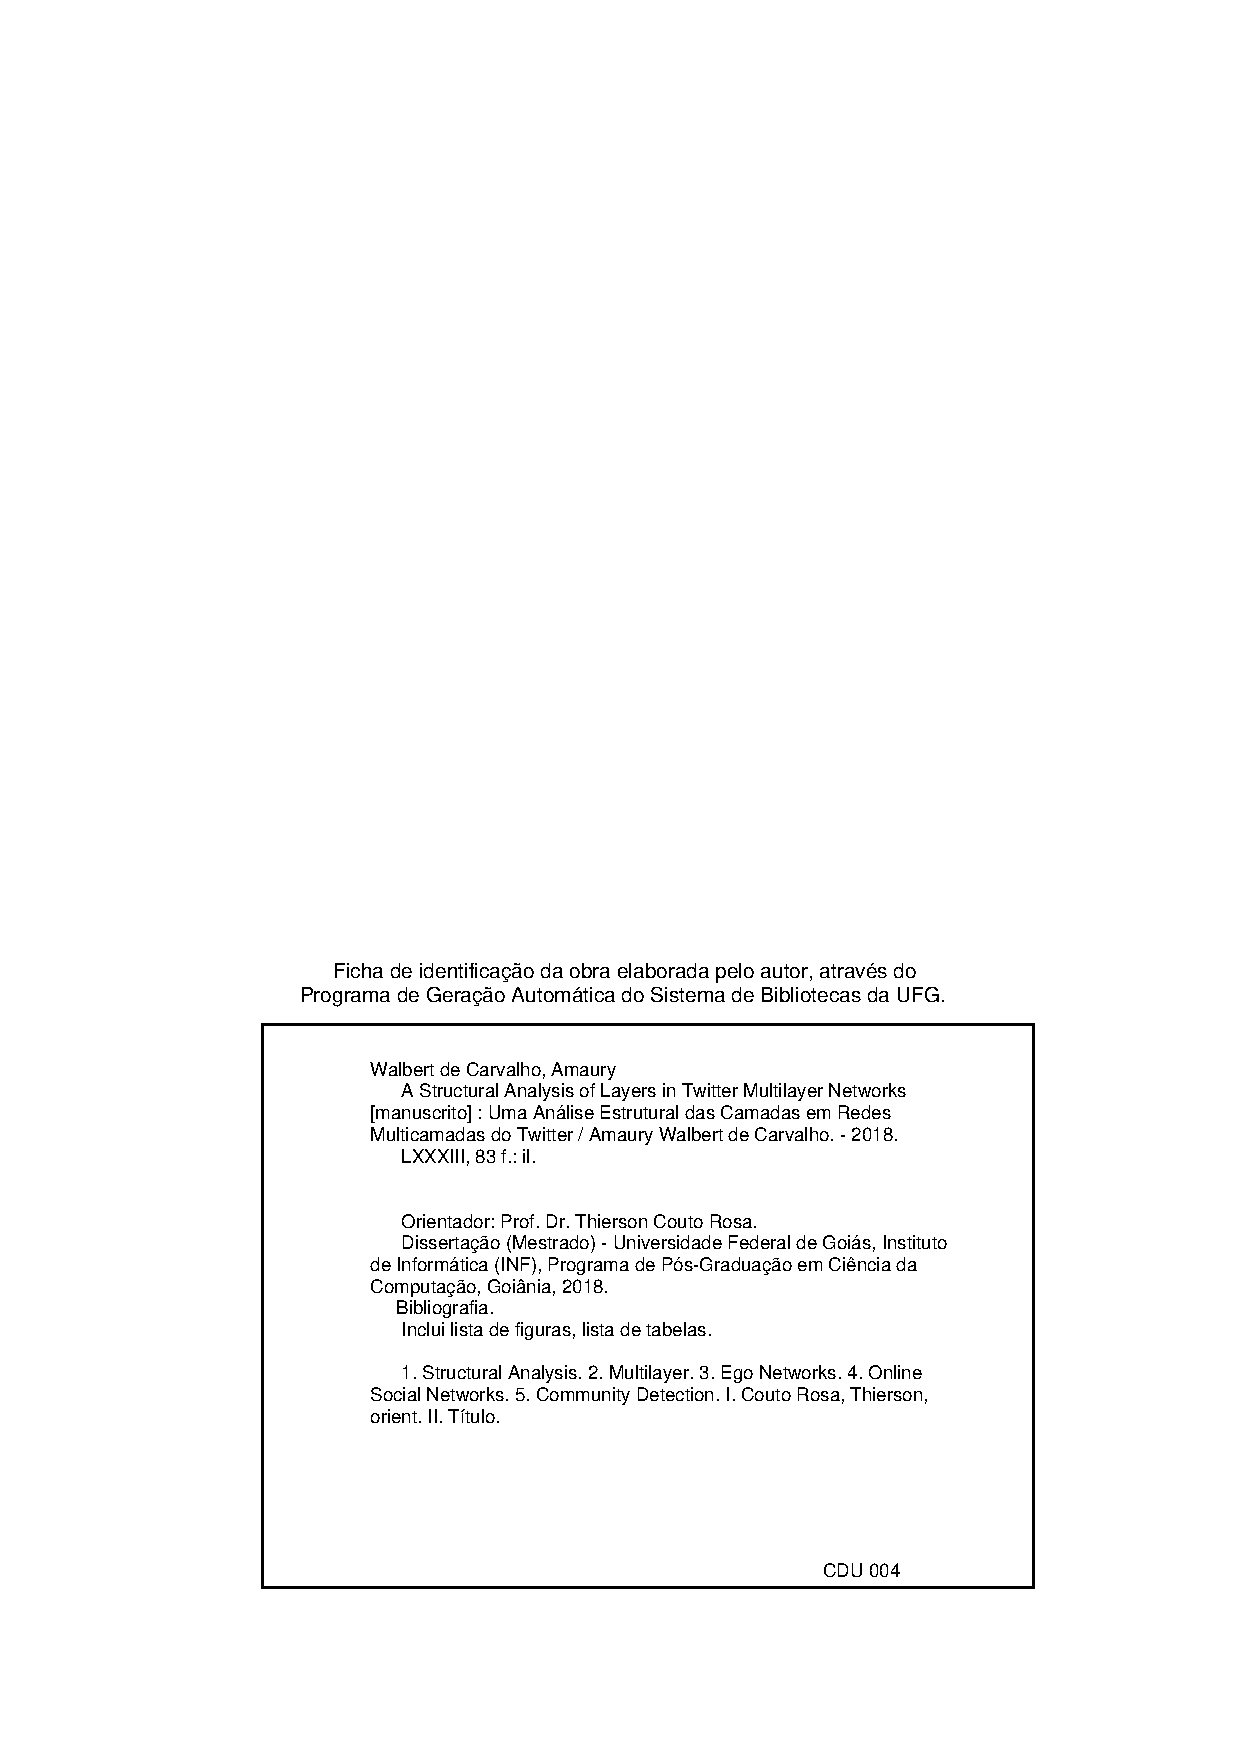
\includepdf[pages={1},templatesize={250mm}{297mm}]{./pre/FichaCatalografica.pdf}
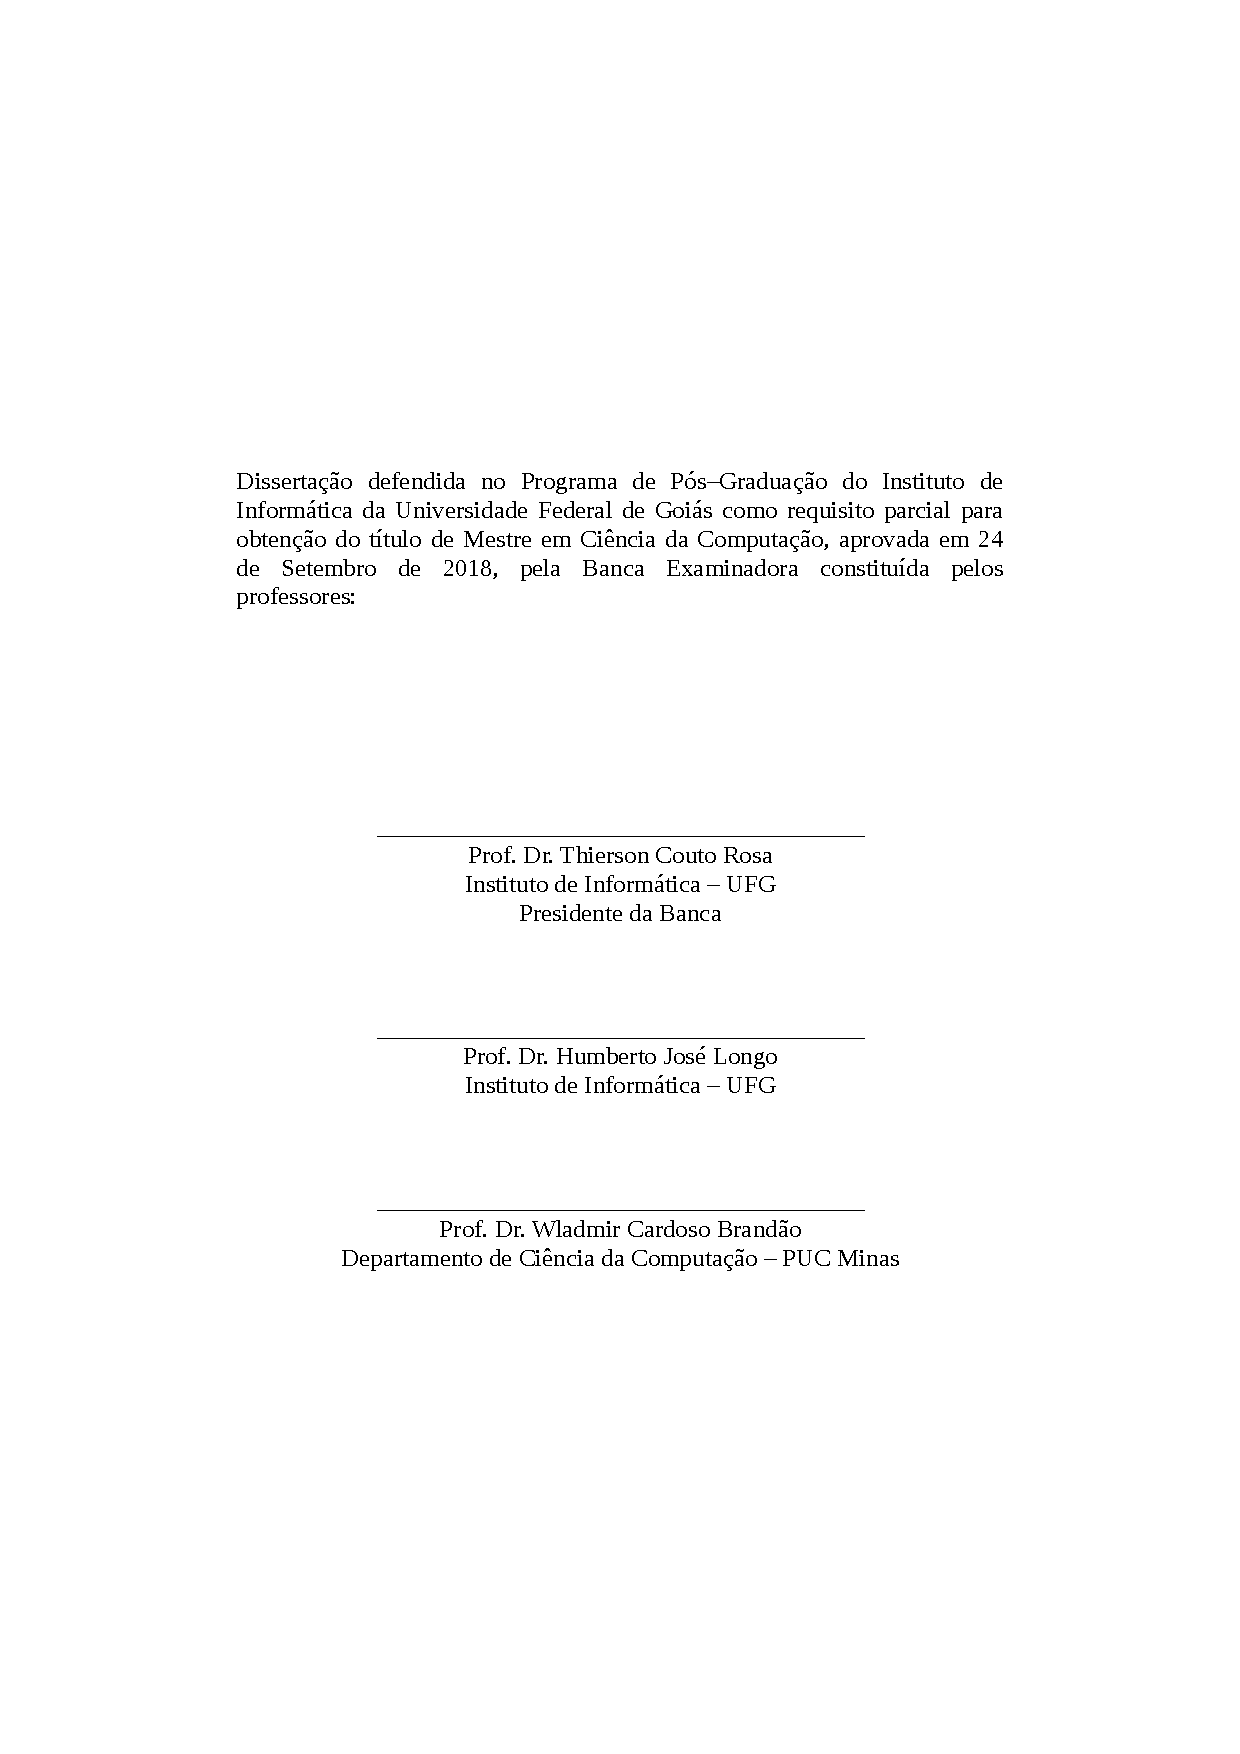
\includepdf[pages={1},templatesize={250mm}{297mm}]{./pre/FolhaAprovacao.pdf}
\direitos{Graduou--se em An\'alise e Desenvolvimento de Sistemas no IF Goiano - Instituto Federal de Educa\c c\~ao, Ci\^encia e Tecnologia Goiano, e em Redes de Computadores na UEG - Universidade Estadual de Goi\'as. Possui especializa\c c\~ao {\em Latu Sensu} em Seguran\c ca em Redes de Computadores pela Faculdade de Tecnologia SENAI de Desenvolvimento Gerencial e em Doc\^encia Superior pela Faculdade Lions. \'E professor efetivo do IF Goiano Campus Uruta\'i e atualmente coordena o Curso T\'ecnico em Inform\'atica Integrado ao Ensino M\'edio.}


\begin{dedicatoria}
Dedico este trabalho ao meu filho, Matias, e a minha esposa, Mayara.
\end{dedicatoria}
\begin{agradecimentos}
Agrade\c co a Deus pela vida e por colocar pessoas maravilhosas no meu caminho que me permitiram desenvolver esse trabalho.

Agrade\c co a minha fam\'ilia, especialmente a minha esposa Mayara, meu filho Matias, meus pais, Antonio e Augusta, meu irm\~ao Almir. Agrade\c co tamb\'em aos meus sogros, Ant\^onio e L\'ucia, e minha cunhada Maryele. Todos me apoiaram de forma incondicional durante do desenvolvimento da disserta\c c\~ao e pude contar com eles em momentos decisivos.

Agrade\c co ao meu orientar, Prof. Dr. Thierson, pela disponibilidade e altru\'ismo, pela dedicação ao projeto e pelo ensinamento oferecido.

Agrade\c co a todos os professores do INF, especialmente os professores Celso e N\'adia, pelas importantes observa\c c\~oes feitas durante o desenvolvimento do projeto.

Agrade\c co a todos os meus colegas de trabalho no IF Goiano que compreenderam e me deram suporte durante o per\'iodo do mestrado.

Agrade\c co a FAPEG pelo aux\'ilio financeiro e ao IF Goiano por ter me proporcionado participar do programa de licen\c ca para capacita\c c\~ao.

Enfim, agrade\c co a todos que de alguma forma contribu\'iram para a realiza\c c\~ao desse projeto.
\end{agradecimentos}



\epigrafe{O maior inimigo do conhecimento n\~ao \'e a ignor\^ancia, \'e a ilus\~ao do conhecimento.}
{Stephen Hawking}
{Astrof\'isico brit\^anico - 1942--2018}

\chaves{Twitter, An\'alise Estrutural, Redes Ego Multicamadas, Detec\c c\~ao de Comunidades.}

\begin{resumo}

O Twitter \'e uma rede social online (RSO) que permite diferentes tipos de  intera\c{c}\~{a}o entre os usu\'arios (ex. ``seguir'', ``retuitar'', ``gostar'', ``mencionar'') e cada tipo de intera\c{c}\~{a}o possui um significado diferente. Entretanto, a maioria do trabalhos que modelam o Twitter como um grafo consideram apenas um tipo de liga\c{c}\~{a}o entre os usu\'{a}rios, notadamente, a intera\c{c}\~{a}o ``seguir''. Al\'{e}m disso, a an\'{a}lise macrosc\'{o}pica  de um grafo  grande como uma RSO  n\~{a}o revela caracter\'{i}sticas particulares do relacionamento dos v\'{e}rtices com suas vizinhan\c{c}as. Nesse  trabalho utilizamos de redes ou grafos ego multicamada para melhor modelar o as intera\c{c}\~{o}es entre um usu\'{a}rio  (o ego) e outros usu\'{a}rios do Twitter.
%O estudo  de v\'{a}rias  redes ego permite detectar repeti\c c\~oes de padrões de comportamento de interação a nível pessoal. A detecção desses  padrões são úteis   para melhorar  servi\c cos personalizados como recomenda\c~{a}o de tweets ou de usu\'{a}rios interlocutores e também para melhorar importantes aplicações em redes sociais como detec\c{c}\~{a}o de comunidades, an\'{a}lise da difus\~{a}o da informa\c{c}\~{a}o, entre outros.
Cada camada (subgrafo da rede ego) corresponde a um tipo espec\'{i}fico de intera\c{c}\~{a}o.  Consideramos  quatro tipos de camadas: {\em seguir}, {\em retuitar}, {\em gostar} e {\em mencionar}. A an\'{a}lise estrutual em 500 redes ego multicamadas nos permitiu verificar interessantes características das redes ego multicamadas do Twitter, tais como: (i) h\'{a} consider\'{a}vel interse\c{c}\~{a}o entre camadas (em termos de v\'{e}rtices e arestas), embora as camadas sejam diferentes entre si; (ii)  a grande maioria das camadas s\~{a}o ``small world'', i.e., a m\'{e}dia dos caminhos m\'{i}nimos \'{e} pequena, mas os coeficientes de agrupamento s\~{a}o altos; (iii) a distribui\c{c}\~{a}o de graus de entrada dos v\'{e}rtices  segue uma lei de pot\^{e}ncia cujo expoente varia entre camadas; (iv) a reciprocidade \'{e} alta na camada ``mencionar'' (superior a 0,4), mas baixa nas demais;
(v) todas as camadas t\^{e}m igual potencial para formarem comunidades.  Os resultados indicam que todas as camadas e as interese\c{c}\~{o}es entre elas possuem caracter\'{i}sticas importantes,   as quais nos  permite sugerir futuras investiga\c{c}\~{o}es nas \'{a}reas de detec\c{c}\~{a}o de comunidades, difus\~{a}o da informa\c{c}\~{a}o  e recomenda\c{c}\~{a}o de tu\'{i}tes. N\~{a}o se tem conhecimento de outro trabalho  que tenha investigado redes ego multicamadas no Twitter. 
\end{resumo}


\keys{Twitter, Structural Analysis, Multilayer Ego  Networks,  Community Detection.}

\begin{abstract}{A Structural Analysis of Twitter Multilayer Ego Networks}


Twitter is an  online social  network (OSN)  that allows users to interact with each other by different interaction types (e.g., ``follow'', ``retweet'', ``like'', ``mention'') and each interaction type has a distinct meaning. However, most researchers that analyze Twitter as graph take into consideration only one interaction type  among users, mainly the ``follow'' interaction. Besides, a macroscopic analysis of a huge graph like an OSN does not reveal intrinsic characteristics of the relationships in a vertex  neighborhood. In this work, we use multilayer ego networks or multilayer ego graphs to better model the interactions between a user (the ego) and other users in Twitter.
Each layer  (a subgraph of the ego network) corresponds to a specific interaction type. We consider  four layer types: {\em follow}, {\em retweet}, {\em like} and  {\em mention}. A structural analysis of 500 multilayer ego networks allowed us to verify interesting characteristics of multilayer ego networks in Twitter, such as: (i) there is considerable overlap between layers (in terms of vertices  and edges), although layers differ from each other; (ii) most layers are    ``small world'', i. e., the mean shortest path in each layer is small, whereas the mean clustering coefficient is large; (iii) indegree distributions follow a power law, with exponent varying among layers; (iv) reciprocity between vertices is high in the follow layer (superior to 0.4), while smaller in the other layers; (v) all the four layers have similar potential to form communities. 
The results of our analysis indicate that all layers and the overlap between them have important characteristics which allowed for suggesting future investigations in the subjects  community detection, information diffusion and retweet recommendation. We do not know of any previous work which has investigated the structural properties of multilayer ego network in Twitter.
\end{abstract}


\tabelas[figtab]
%Opções:
%nada [] -> Gera apenas o sumário
%fig     -> Gera o sumário e a lista de figuras
%tab     -> Sumário e lista de tabelas
%alg     -> Sumário e lista de algoritmos
%cod     -> Sumário e lista de códigos de programas
%
% Pode-se usar qualquer combinação dessas opções.
% Por exemplo:
%  figtab       -> Sumário e listas de figuras e tabelas
%  figtabcod    -> Sumário e listas de figuras, tabelas e
%                  códigos de programas
%  figtabalg    -> Sumário e listas de figuras, tabelas e algoritmos
%  figtabalgcod -> Sumário e listas de figuras, tabelas, algoritmos e
%                  códigos de programas

%--------------------------------------------------------------- CAPÍTULOS %
\chapter{Introduction}
\label{cap:Intro}

In the past few years network theory has been largely and successfully used in the investigation and characterization of the structure and dynamics of complex systems \cite{Strogatz2001, Newman2003}. The research challenge has been the improvement of techniques that allow the understanding of the structure and behavior of the elements of real systems, which attracts researchers from diverse fields of knowledge such as biology, sociology, mathematics, physics, computer science, among others \cite{Motter2012,Orman2012,Zafarani2015,Chakraborty2017}.

The most widely used model for representing complex systems is through graphs. The traditional network theory represents each constituent elementt (or unit) of a complex system as node of a graph and all the interactions or relationships between two units as a single link, i.e, an edge in the graph. With this model it is possible to determine some non-trivial topological (structural) features of a complex system such as small-worlds or scale-free, and exhibit community structures \cite{PARK201632}.

Despite not taking into consideration specificities among the different types os interactions or relationships, the modeling approach of complex networks through graphs has been extremely successful. For instance, it has been used to show that many real networks present the small-world property \cite{Watts1998, Porter:2012}, the high clustering coefficient and low values for the shortest path lenght; scale-free due to the heavy-tailed degree distribution \cite{Barabasi509, Clauset2009}; and  contain nodes that play central roles as authority or popularity \cite{Newman:2010, Wasserman1994}, among other important findings.

%%%%%%%%%%%%%%%%%%%%%%%%%%%%%%%%%%%%%%%%%%%%%%%%%%%%%%%%
%%%%%%%%%%%%%%%%%%%%%%%%%%%%%%%%%%%%%%%%%%%%%%%%%%%%%%%%


\section{Motivation}
\label{sec:motivation}

Modeling all types of relationships and interactions between two nodes as a single link between them might in general discard important information about the structure and function of the original system, because in many cases these interactions differ both in meaning and in intensity \cite{Darmon2015}. On the other hand, failure to evaluate the importance of each different type of relationship between two vertices results in a poor representation of the system \cite{Szell2010}. For example, in complex multimodal transportation systems, a set of locations might be reached in different ways, e.g., using bus, underground, suburban rail, and other types of transportation. In these systems, each type of interaction (i.e., type of transportation between locations) has associated a given relevance, importance, cost, distance and limitation.

In online social networks (OSNs), like Twitter, a user may interact with other users in different ways, e.g., by following another user, by liking a tweet of another user, by retweeting a tweet written by another user and by mentioning  other user. Each of these interaction types has a different meaning. Also, some of them do not naturally have an associate value or weight (ex. the following relation) while others have (e.x.,  user $a$ may have retweet  user $b$ 50 times). Thus, treating all the links as being equivalent implies in losing  important information.  

A more appropriate modeling of such systems is in terms of  a network with many layers where  each layer describes all the edges of a given type. Informally, a {\em multilayer network}  is a  set of $n$ nodes which are connected to each other by means of edges belonging to $m$ different classes or types. Each class of edges is represented as a separate layer. \thierson{One may consider that a node $i$ of the multilayer network consists of $k$, $1\leq k \leq m$ replicas, one for each layer that $i$ is involved in.} 

Recently, a great effort has been devoted to the characterization and modeling of multilayer networks. There are many types of modeling multilayer networks. Consequently, some  measures have been proposed in the context of real-world multilayer networks such as multiplayer online games \cite{Szell2010}, air transportation systems \cite{Cardilo2013}, and Indonesian terrorist network \cite{Battiston2014}. 

Twitter is a very important OSN not only because it is an information diffusion media used by millions of people including journalists, artists and presidents of many countries, but also because it is the most  investigated OSN by academic researchers. Many research about Twitter has emerged  involving a pletora of applications like, for example, information cascading analysis \cite{HU2017, Hakim2014}, influence detection \cite{Chen:2014,Haddadi2010}, community detection \cite{McAuley:2012,GADEK2017584}, content recommendation \cite{Hong:2013,Chen2012,Jiang:2016} among others.

However, the different types of interaction among Twitter users have rarely been studied as separate layers of the Twitter network in literature. Actually, worse than treating different types of interactions in the same way, the majority of research about Twitter has considered only the {\em follow} interaction as connections among users. The other types of interaction are neglected or are considered only as additional information over the structure of the network formed by the {\em follow} links. 

In Darmon et al. \cite{Darmon2015} we have an example of this "following restricted" view of Twitter, by proposing a multifaceted approach to detect communities in Twitter. The authors analyzed three different facets: user activity, topic and interaction (retweet or mention). However, they  the build a graph based on the follow interaction among users and derive distinct versions of this graph by assigning  to edges a different weight related to each facet of the communities  they intend to detect.

Another example, Bhattacharya et al. \cite{Bhattacharya:2014} propose an approach to identify topic of interest of given Twitter user $u$ by first identifying the topics of interest of people $u$ follows. They showed that their approach is promising, but an interesting question is if even better results could be achieved if interaction links related to users explicit approval reaction (like or retweet) were considered instead the following relation. 


%%%%%%%%%%%%%%%%%%%%%%%%%%%%%%%%%%%%%%%%%%%%%%%%%%%%%%%%
%%%%%%%%%%%%%%%%%%%%%%%%%%%%%%%%%%%%%%%%%%%%%%%%%%%%%%%%


\section{Justification}
\label{sec:justification}

Only recently, researchers started considering a multi-relational or multilayer view of the relations in Twitter \cite{Azaza2015,Zhaoyun2013,Hajibagheri2016}. The works in \cite{Azaza2015, Zhaoyun2013} investigated how to detect influence users in Twitter by considering the Twitter network as formed by layers. The work in \cite{Hajibagheri2016}, proposed a method for predicting links in a multilayer network derived from Twitter, composed of three layers corresponding to reply, retweet and mention interactions.

These articles take advantage of considering Twitter as a multilayer network in specific applications. However, there are only few articles which analyze the characteristics of the different layers in Twitter, as well as the difference among these layers \cite{Omodei2015}. Research in this direction is very important because it can reveal useful structural information about the layers that may influence design of solutions of many applications like tweet recommendation, sentiment analysis, user profiling for market analysis, among others.

In this work, we adopt a user-based approach to investigate multilayer networks derived from Twitter. For a given user $e$ (the {\em ego}), we derive her ego network by obtaining her interactions with other users in Twitter. We consider user $e$ and each user she interacts with as the nodes of her ego network. We refer to each user $e$ interacts with as $e$'s {\em alter}. The set of direct edges in the ego network is composed of interactions among the set of users formed by the ego and the alters. For each ego network we define a layer for four different interaction types: {\em follow, retweet, like} and {\em mention}. A formal definition of a multilayer ego network is given in Section \ref{sec:MEN}.

The adoption of an egocentric point of view for investigating the different layers of Twitter is interesting for many reasons including: 
\begin{itemize}
\item [a)] It allows for obtaining different small samples of the Twitter network which is convenient for detecting repetitions of patterns or tendencies in the whole network \cite{Leskovec2012}. 
\item [b)] It reveals important aspects that may be useful for research in many critical personalized services on OSNs, such as personalized recommendation \cite{Hong:2013,Chen2012}, detection of influential users for a target user \cite{Guo:2013}, and local community detection \cite{McAuley:2012,Coscia:2014}, to name a few.  
\end{itemize}

Contrary to the work found in the literature that analyzes only a small set of ego networks \cite{Achiam2016,Omodei2015,Leskovec2012,Epasto2015,Dykstra2014}, usually in a specific context, we use for this work an extensive set of 500 ego networks collected from Twitter. This collection gives us an overview of the behavior of egos in each layer, that is, Twitter users, not just the behavior between a specific ego and its set of alters. For example, by analyzing the variability of each ego's interactions at each layer, we can identify whether there is a uniform distribution of different types of interactions or whether Twitter users tend to use a particular type of interaction, among other possibilities.

Another point that deserves attention in the analysis of OSNs is in relation to the quality of the communities present in these networks. When we treat a Twitter ego network as a multilayer network we are considering different approaches to building the layers rather than just explicit connections between users such as ``follow'' on Twitter. Detecting communities in different layers results in communities with different meanings, based on the type of interaction between users. According to Darmon et al. \cite{Darmon2015}, the concept of community is very broad and the goal of community detection must be in line with the type of community one wishes to encounter. In this direction, multilayer analysis expands the possibilities of improving the quality of the communities found in OSNs.

For this work we have collected the public data of Twitter users with egos selection criteria based on the Twitter lists in which they are registered or are the owners. The intention of this type of collection is not to let the data be biased on one of the interactions that we consider as one of the layers of the modeled multilayer ego networks. In addition, the collection of this form allows us to verify if this resource (Twitter lists) can be used as ground-truth for the problem of detecting communities, since there is a difficulty to find labeled communities to evaluate the quality of the communities detected in these network \cite{Xie2013,Wang2014,Zafarani2014,Zafarani2015}.

%%%%%%%%%%%%%%%%%%%%%%%%%%%%%%%%%%%%%%%%%%%%%%%%%%%%%%%%
%%%%%%%%%%%%%%%%%%%%%%%%%%%%%%%%%%%%%%%%%%%%%%%%%%%%%%%%


\section{Objectives}
\label{sec:objectives}
This work has as general objective to perform a structural analysis of the Twitter multilayer ego networks from the evaluation of structural properties in each layer. Specific objectives are:

\begin{itemize}
    \item Identify the main layers and perform the collection of a set of Twitter multilayer ego networks.
    \item Analyze how do the number of edges and the number of vertices vary among layers.
    \item Find out how reciprocal relations are in each layer.
    \item Check for similarities in the elements (vertices and edges) and topology of the layers.
    \item Identify if the layers are scale-free networks.
    \item Identify if the layers are small worlds networks.
    \item Investigate the capacity of the layers to generate communities.
    \item Discover how a Twitter user relates to the users who are associated with their lists.
\end{itemize}


%%%%%%%%%%%%%%%%%%%%%%%%%%%%%%%%%%%%%%%%%%%%%%%%%%%%%%%%
%%%%%%%%%%%%%%%%%%%%%%%%%%%%%%%%%%%%%%%%%%%%%%%%%%%%%%%%


\section{Main Contributions}
\label{sec:contributions}
We do not know of any work that analyzed the structural properties of different layers composing the ego networks in Twitter before. We consider that, in investigating the research objectives, described above, this work presents important contributions to understanding the network around a person on Twitter. The contribution of this dissertation are summarized as follows:

\begin{itemize} 
%    \item We investigated the distribution of the size of the vertex and edge sets in the follow, retweet, like and mention layers. All the layers presented high variance in the number of vertices and edges between the ego networks. As for the vertex set size, the retweet and like layers maintain a strong positive correlation and tend to converge to an average size, while the follow and mention layers have a moderate positive correlation and exhibit a long tail distribution.

    \item We found  great variation in the number of vertices and edges among different layers for the same ego and for different egos. However,  the greatest majority of layers have very low density and the density values do not differ much from one layer to another. Also, in most layers the majority of edges are not ego-alter edges meaning that there is many interactions from alters to other alters and from alters to the ego.

    \item For most ego networks, layers  differ from each other in both the vertices and the edges composing them. However, there are some overlap between layers. Specially, there is overlap between the most important vertices in each layer.

%    \item We have identified that analyzed ego users tend to mention users that they follow, and that they tend to mark as favorite the tweets posted by users that they retweet (and vice versa). However, retweets and likes are usually performed on user tweets that the ego does not follow or mention.

%    \item We also analyzed edge overlap among layers and found that the amount of edge overlap between pairs of layers  is small for all pairs considered. This occurs because despite the great amount of overlap of interactions between the ego and her alters, the alters do not interact with the same intensity and same patter with each other in each layer, which leads to a small intersection of the set of edges between layers.

%    \item Many users (egos) may not receive all the tweets produced by the alters they interact most by retweets, likes and mentions. We found that ego users could retweet more if they were following their main retweet layer alters, because they retweeted a considerable number of tweets from users who are not their friends so there may be more tweets that they could retweet but end up not arriving in your timelines automatically, affeting information cascading in Twitter.
    
    \item  Most layers are scale-free and are small world graphs. These are  interesting novelties, since only the follow layer was supposed to have these properties given that they were found in previous work that considered samples of the entire Twitter follow graph \cite{Aparicio2015}.
    
%    \item We note that the distribution of indegrees of all layers of all ego networks follows a power law, and practically all layers of ego networks are small-worlds. The clustering coefficient of the mentions layer was larger than the other layers.

    \item  Vertices in all  layers have high clustering coefficient, which means that they tend to cluster into communities. In fact, we found that all type of layers in most ego networks are structured in interconnected communities which follow similar patterns in all layers. This findings are very interesting because community detection has been applied only to networks formed by the follow interaction. We show that other type of interactions have similar potential to be used for community detection in Twitter.    
    
%    \item From the analysis made on the detected communities we can conclude that the distribution of values of all measures are surprisingly very similar for all layers. This information suggests that  the retweet, like, and mention layers have the same potentiality to be used for community detection in ego networks in Twitter as has the follow layer.
    
 %   \item We present a new approach to the problem of communities detection in Twitter because the different layers give the opportunity to evaluate the quality of the communities both according to the structure of the graph (follow layer) and according to the content or topics of the messages (retweet, like and mention layers).
    
    \item We show that there is little interaction between the ego and the elements of the Twitter lists, so it is not possible to use the lists as ground-truth in the process of assessing the quality of the communities detected in the ego networks.
    
    \item  We present a discussion on how the above findings and others reported in this article may be useful for  important applications in Twitter, like community detection and information diffusion.  

\end{itemize}

%%%%%%%%%%%%%%%%%%%%%%%%%%%%%%%%%%%%%%%%%%%%%%%%%%%%%%%%
%%%%%%%%%%%%%%%%%%%%%%%%%%%%%%%%%%%%%%%%%%%%%%%%%%%%%%%%


\section{Organization of Text}
\label{sec:organization}

The following is the layout of the contents of the remainder of this dissertation. Chapter \ref{cap:Basic} presents some basic concepts, definition and analysis of the network structure, and the details about the properties and measures of networks that we use to achieve the proposed objectives. In Chapter \ref{cap:RW} the main works related to this dissertation are described.

Chapter \ref{cap:ExpSetup} defined the Twitter multilayer ego networks that were the objects of our study. Also in Chapter \ref{cap:ExpSetup} we describes the procedures for collecting and preparing the data for the experiments, as well as the configuration used in the modeling of the layers of the ego multilayer networks. In Chapter \ref{cap:Results} we present the results of the experiments, and in Chapter \ref{cap:Considerations} is the text with the final considerations of the work.

\chapter{Basic Concepts}
\label{cap:Basic}

Most real networks, like social, biological, and technological networks present many non-trivial topological features, with patterns of connection between their elements that are neither purely regular nor purely random. These features include the scale-free, the small-world and community structure properties. In this work we are interested in investigating whereas these properties occur in Twitter multilayer ego networks. Besides, we are also interested in analyzing similarities and dissimilarities among layers of the multilayer ego networks considered. Thus, in this chapter we present the concepts and the related measures we use to answer our main research questions.

At the outset, section \ref{sec:graphs} is the definition of graphs, with their main characteristics. Graphs are mathematical models used in this work for the representation of multilayer ego networks. In section \ref{sec:graph_properties}, we list some of the main properties of graphs and how they are used in the network analysis process. In section \ref{sec:net_models} are described some models that represent phenomena found in the real networks and that help to understand the structures of the networks. In sections \ref{sec:important_vertices} and \ref{sec:vertex_edges_overlap} we investigate the similarity between the layers of the same multilayer ego network. Finishing this chapter, the section \ref{sec:communities} is devoted to describing concepts that involve one of the major structures exhibited by OSNs, the communities, approaching detection algorithms and evaluation metrics of these structures in graphs.


%%%%%%%%%%%%%%%%%%%%%%%%%%%%%%%%%%%%%%%%%%%%%%%%%%%%%%%%
%%%%%%%%%%%%%%%%%%%%%%%%%%%%%%%%%%%%%%%%%%%%%%%%%%%%%%%%

\section{Graphs}
\label{sec:graphs}

Graphs can be understood as mathematical models used to represent relationships between objects of a given set and is usually used to model network structures. The notation of a graph $\mathcal{G}$ can be developed as a set of vertices $\mathcal{V}$, representing the objects of a network, and a set of edges $\mathcal{E}$ that connect the vertices and represent the relationships between the pairs of objects. Mathematically speaking, the graph $\mathcal{G}$ is expressed by Eq. \ref{eq:graph}:

\begin{equation} 
    \label{eq:graph}
    \mathcal{G}=(\mathcal{V},\mathcal{E}),
\end{equation}

where $\mathcal{V}$ is the set of vertices $\mathcal{V}=\{v_1, v_2, . . . , v_n\}$, with $v_i, 1 \leq i \leq n$ being a single vertex; and $\mathcal{E}$ is the set of edges $\mathcal{E}=\{e_1, e_2, . . . , e_m\}$, with $e_i, 1 \leq i \leq m$, being a single edge. 

The edges are formed by a tuple $e(v_1,v_2), v_1, v_2 \in \mathcal{V}$ which indicates a connection between the vertices $v_1$ and $v_2$. Since the edges connect two vertices, we have $\mathcal{E} \subseteq \mathcal{V} \times \mathcal{V}$. The number of vertices $|\mathcal{V}|$ indicates the {\em order} of the graph and the number of edges $|\mathcal{E}|$ indicates the {\em size} of the graph.

The vertices of a graph can also be called nodes or actors depending on the context and subject in which they are being used. In this dissertation we will use the term {\em vertices} to refer to the set of objects modeled in graphs. In OSNs the set of vertices represents the entities, or generally called users, that is, people, companies, computer systems, etc., that create and manage profiles in the virtual environment made available by OSNs; and the set of edges represent the interactions that take place between these users. For example, the graph shown in Fig. \ref{fig:ex_graph_undir} models the friendship relationship between seven users of a fictional OSN. Each user is represented by a vertex, drawn as a circle. There is an edge between two users only if they maintain a friendly relationship in OSN. A line connecting two vertices is the representation of an edge.

\begin{figure}[htb]
	\centering
	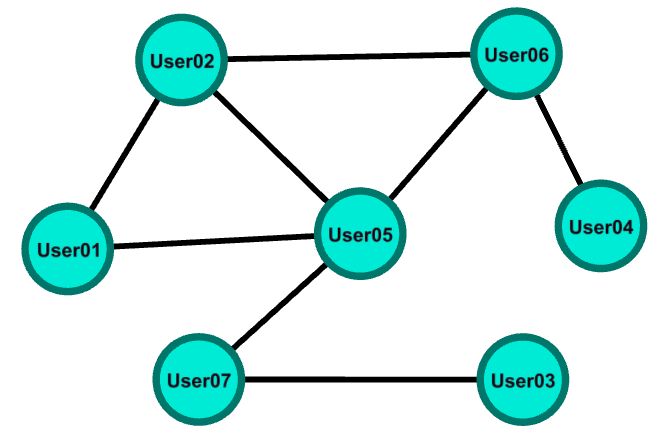
\includegraphics[width=0.8\textwidth]{fig/intro/ex_graph_undir.png}
	\caption{Example of a graph representing the friendship relationship between users of an OSN.}
	\label{fig:ex_graph_undir}
\end{figure}

The friendship interaction represented in Fig. \ref{fig:ex_graph_undir} indicates that each pair of users are friends when there is an edge linking them, or they are not friends if there is no edge linking them. This means that in the example cited, user {\em User01} is friend of user {\em User02} and vice versa. The graph that models this type of relationship is called an undirected graph, and the edges are formed by unordered pairs of vertices that model a bidirectional relationship. In an undirected graph $\mathcal{G} = (\mathcal{V}, \mathcal{E})$, the edge $e(a,b)$, $a, b \in \mathcal{V}$ is the same edge $e(b,a)$, $a, b \in \mathcal{V}$.

Graphs can also be used to model unidirectional relationships between vertices pairs. Sending a message from user $a$ to user $b$ on an OSN, for example, is a type of one-way relationship. In cases like these, the constructed graph should show the direction of the relationships. These graphs are called directed graphs, digraphs, and an edge, which can also be called an arc, is formed by an ordered pair of vertices, called initial vertex (tail) and terminal vertex (head). In this dissertation we will use only the term {\em edges} to refer to the connection between two vertices of a graph. The representation of the edges is made by arrows that start from an initial vertex and arrive at a terminal vertex (head). In a directed graph $\mathcal{G} = (\mathcal{V}, \mathcal{E})$, the edge $e(a,b)$, $a, b \in \mathcal{V}$ is different from the edge $e(b,a)$, $ a, b \in \mathcal{V}$.

\begin{figure}[htb]
	\centering
	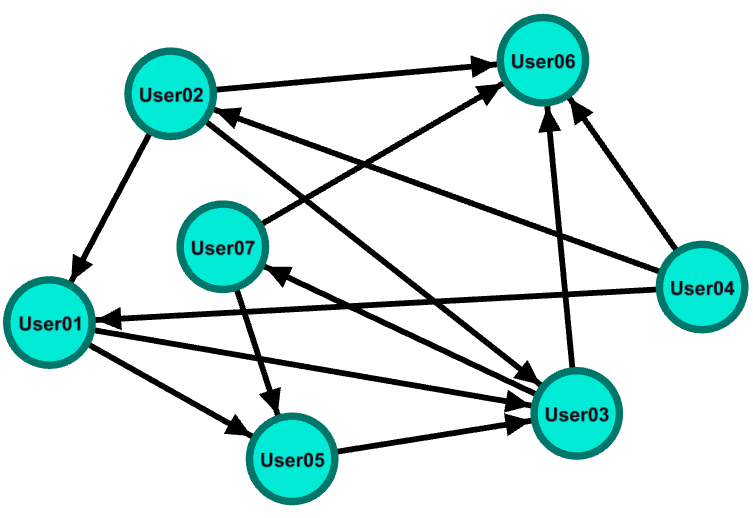
\includegraphics[width=0.8\textwidth]{fig/intro/ex_graph_dir.png}
	\caption{Example of a directed graph representing relationships arising from message sending interactions between users of an OSN.}
	\label{fig:ex_graph_dir}
\end{figure}

The Fig. \ref{fig:ex_graph_dir} illustrates the example of a directed graph that models interactions associated with sending messages between users. In this type of interaction, there is the definition of a sender, user that promotes the interaction, that is, the initial vertex of the edge, and a recipient, who receives the message and is the terminal vertex of the edge. Therefore, it is necessary for the edge to indicate the flow of information to represent the interaction in a correct way, different from the example with the friendship interaction, in which the edge only needs to indicate whether there is interaction (friendship) or not.

Two vertices are {\em adjacent} if they are connected by an edge. Adjacency can also be referenced as {\em neighborhood}. The adjacent vertices (neighbors) of a vertices $a$ form the neighborhood of $a$. In the case of a directed graph, the neighborhood is divided into: (i) successors - the vertex $b$ is successor of $a$ if there is an edge that starts from $a$ and arrives at $b$; and (ii) predecessors - the vertex $a$ is the predecessor of $b$ if there is an edge that goes from $a$ to $b$. The notation used for the neighborhood of a vertex $a$ in a graph $\mathcal{G}$ is represented by Eq. \ref{eq:neighborhood}:


\begin{equation} 
    \label{eq:neighborhood}
    N_\mathcal{G}(a)
\end{equation}

and is called the open neighborhood of $a$ when $a$ is not enclosed, or closed neighborhood of $a$ when $a$ is enclosed. The vertices neighborhood can be used to represent graphs in computer algorithms and are also used to identify properties of graphs.

Graphs can also have subgraphs. A subgraph of $\mathcal{G}$ is a graph whose set of vertices is a subset of the set of vertices of $\mathcal{G}$ and the set of edges is a subset of the set of edges of $\mathcal{G}$. Formally we have that for any graph $\mathcal{G}=(\mathcal{V},\mathcal{E})$ a graph  $\mathcal{G'}=(\mathcal{V'},\mathcal{E'})$ is a subgraph of  $\mathcal{G}=(\mathcal{V},\mathcal{E})$ if it holds the following properties:

\begin{itemize}
    \item $\mathcal{V'} \subseteq \mathcal{V}$,
    \item $\mathcal{E'} \subseteq (\mathcal{V'} \times \mathcal{V'}) \cap \mathcal{E}$.
\end{itemize}

One can traverse a graph starting from one point to another through paths formed by vertices and edges. A distance $k$ between two vertices $a$ and $b$, is defined as $p(a,b)_k$, and is an alternating sequence of vertices and edges that starts at $a$ and ends in $b$, according to Eq. \ref{eq:path_lenght_k}:

\begin{equation}
    \label{eq:path_lenght_k}
    p(a,b)_k = v_0,e_1,v_1,e_2,v2,...,e_k,v_k
\end{equation}

such that, (i) $a=v_0$ and $b=v_k$; (ii) there is at least one edge; (iii) for $1 \leq i \leq k$ the edge $e_i$ connect the vertices $v_{i-1}$ and $v_i$.


If the graph is undirected, the vertices that are bounded by the $e_i$ edge are $v_i$ and $v_{i+1}$, otherwise, $e_i$ is an edge that starts from $v_i$ and ends in $v_{i+1}$. The length of the walk is defined by the number of edges that it has, or, in weighted graphs, by the weight of the edges of the path, which also corresponds to the distance of the path. A walk that does not pass twice through the same vertex is called {\em path}. A walk that begins and ends at the same vertex and there are no repeated edges is called {\em circuit}, and a circuit that does not have repeated vertices is called {\em cycle}.

For a directed graph $\mathcal{G}$, we say that $C_{a,b}$ is a shortest path between vertices $a$ and $b$ if there is no other path that starts at $a$ and ends at $b$ (or vice versa in undirected graphs) of lesser length that $C_{a,b}$, that is, $C_{a,b}= min(p(a,b))$. If there is no path from $a$ to $b$, we can say that the distance from $a$ to $b$ is infinite.

%%%%%%%%%%%%%%%%%%%%%%%%%%%%%%%%%%%%%%%%%%%%%%%%%%%%%%%%
%%%%%%%%%%%%%%%%%%%%%%%%%%%%%%%%%%%%%%%%%%%%%%%%%%%%%%%%


\section{Graph Properties}
\label{sec:graph_properties}
The analysis of a network passes through the understanding of its structure, which can be made from the graphs teory, according to the properties exhibited by them. The properties analyzed allow us to evaluate the graph for aspects related to its vertices and connections, for example, to determine which are the central vertices, shortest paths between the vertices, degree of connection of the vertices, etc. In OSNs, the analysis of these properties is essential for the correct understanding of the dynamics of formation of communities, such as the identification of cohesive groups, their central vertices, vertices of connection with other groups, estimation of the flow of information transmitted between vertices, etc. Here are some of the main properties of graphs:

\begin{itemize}
	\item \textbf{Order -} the order of a graph represents the number of vertices in the graph: $o(G) = |\mathcal{V}|$.
        	
    \item \textbf{Size:} the size of a graph is indicated by the number of vertices plus the number of links between them: $s(G) = |\mathcal{V}| + |\mathcal{E}|$.
        
    \item \textbf{Average Degree -} Indicates the number of connections that, on average, each vertex of the graph has. In the case of OSNs, this measure must be interpreted with caution because the degree distribution generally does not follow a normal distribution, as it was possible to observe in Fig. \ref{fig:twitter_degree_distr}, therefore, the average has no representativity. However, even so, this propertie helps in comparing different networks. The average degree is defined according to Eq. \ref{eq:avg_degree}:
    \begin{equation}
        \label{eq:avg_degree}
    	d(G) = \frac{1}{|\mathcal{V}|} \sum_{v \in \mathcal{V}}d_G(v).
    \end{equation}
        
	\item \textbf{Eccentricity -} the eccentricity of a vertex $v$ corresponds to the maximum distance between $v$ and any other vertex $u$ of the graph: $e(v) = max_{u \in \mathcal{V}}d(u,v)$.

    \item \textbf{Diameter -} The diameter of a network represents the largest distance between two vertices of the network, that is, the greatest eccentricity. This propertie is useful for evaluating the maximum distance an information would need to travel to reach two vertices in a network using only shortest paths, that is, it reveals the number of minimum connections required to connect two vertices of the network. It is calculated by observing the greatest of all shortest paths between the vertices, according Eq. \ref{eq:diameter}:
    	\begin{equation}
    	    \label{eq:diameter}
        	d = max_{v \in \mathcal{V}}e(v).
    	\end{equation}
        
    \item \textbf{Radius -} the radius of the network is equal to the shortest path between two vertices, that is, the smallest eccentricity: $r = min_{v \in \mathcal{V}}e(v)$.
            
    \item \textbf{Center -}: A vertex $v$ is in the center of the network if the radius of the network is equal to the eccentricity of the vertex $v$: $e(v) = r$.
        
    \item \textbf{Periphery -} A vertex $v$ is at the periphery, if its eccentricity is equal to the diameter of the network: $e(v) = d$.
    	
    \item \textbf{Density -} The density of a network is defined as the ratio of edges to the number of possible edges. For directed graphs the density is calculated according Eq. \ref{eq:density_directed}:
        \begin{equation}
            \label{eq:density_directed}
            D=\frac {|\mathcal{E}|}{|\mathcal{V}|(|\mathcal{V}|-1)}.
    	\end{equation}
    
    For undirected graphs, each edge must be counted twice, according Eq. \ref{eq:density_undirected}:
        \begin{equation}
            \label{eq:density_undirected}
            D=\frac {2|\mathcal{E}|}{|\mathcal{V}|(|\mathcal{V}|-1)}.
    	\end{equation}
\end{itemize}

\subsection*{Degree Centrality}
\label{subsec:degree_centr}
The degree centrality of a vertex $a$ is defined as the number of edges associated with it ($d_a$), which also corresponds to the number of adjacent vertices. A zero-degree vertex is called an isolated vertex. In unirected graphs, the sum of the degrees of all vertices is equal to twice the number of edges of the graph, according to Eq. \ref{eq:node_degree_undirected}:

\begin{equation} 
\label{eq:node_degree_undirected}
    \sum_{i}d_i = 2\left | \mathcal{E} \right |,
\end{equation}

since each edge links two vertices. In directed graphs, the degree of a vertex $a$ is decomposed into {\em indegree} ($d_a^{in}$) and {\em outdegree} ($d_a^{out}$), the which corresponds, respectively, to the number of edges that arrive at the vertex, that is, the number of edges in which the vertex $a$ is the terminal vertex, and the number of edges that start from the vertex, that is, the number of edges where $a$ is the initial vertex. Therefore, the degree of a vertex $a$ is formed by the sum of the indegree and the outdegree, as Eq: \ref{eq:node_degree_directed}:

\begin{equation} 
\label{eq:node_degree_directed}
    d_a = d_a^{in} + d_a^{out},
\end{equation}

and the sum of all indegrees is equal to the sum of all outdegrees, in accordance with Eq. \ref{eq:node_degree_directed_total}:

\begin{equation}
\label{eq:node_degree_directed_total}
    \sum_{i}d_i^{in} = \sum_{j}d_j^{out}.
\end{equation}

A special case of binding in a graph is the {\em loop}, which occurs when an edge attaches a vertex to itself. In undirected graphs, each loop adds two to the degree of the vertex that owns it, as this will be identified as initial vertex and terminal vertex for the edge of the loop. It is worth remembering that in the case of a directed graph, each loop will add one to the indegree and one to the outdegree of the vertex that owns it.

When working with graphs of the order of thousands of vertices, or even larger than this, it is important to evaluate initially the distribution of degrees of vertices. The distribution $p_d$ is the probability that a randomly selected vertex has degree $d$. In a graph with $n$ vertices, $p_d$ is defined according to Eq. \ref{eq:prob_degree}:

\begin{equation}
    \label{eq:prob_degree}
    p_d = \frac{n_d}{n},
\end{equation}

where $n_d$ is the number of vertices with degree $d$. Figure \ref{fig:twitter_degree_distr} gives the example of the probability distribution through the representation of the Twitter mentions network in April 2017\footnote{\textit{Twitter network dataset - KONECT, April 2017}. \url{http://konect.uni-koblenz.de/networks/munmun_twitterex_at}}. Each vertex of this network is a Twitter user and a directed edge indicates a direct message sent from one user to another. The degree of each vertex is given by the sum of the indegree and the outdegree. It can be observed that, in this example, most users have a very low degree, while a much smaller number of users have a high degree.

\begin{figure}[htb]
	\centering
	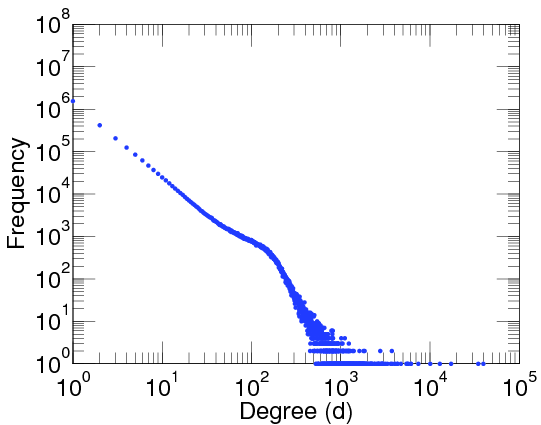
\includegraphics[width=0.8\textwidth]{fig/intro/twitter_degree_distr.png}
	\caption{Distribution of degrees from the Twitter mentions network - April 2017.}
	\label{fig:twitter_degree_distr}
\end{figure}


\subsection*{Betweenness Centrality}
\label{subsec:betweenness_centr}
The betweenness centrality evaluates the importance of the vertices and edges as to the capacity to serve as a link between the elements of the network. One of the ways of calculating the centrality of intermediation is presented in \cite{Zafarani2014}, in which the authors demonstrate that for a given vertex $v$, we compute the number of shortest paths between two other vertices that pass through vertex $v$, according to Eq. \ref{eq:spl}:

\begin{equation}
    \label{eq:spl}
    C_b(v) = \sum_{s \neq t \neq v} \frac{\sigma_{st}(v)}{\sigma_{st}},
\end{equation}
        
where $\sigma_{st}$ is the minimum number of paths from $s$ to $t$ and $\sigma_{st}(v)$ is the number of shortest paths from $s$ to $t$ that pass through $v$. The same approach can also be used to calculate the edge betweeness centrality. In the case of directed graphs, the direction of the edges must be considered.

For the case of comparison between different networks, the betweenness centrality must be normalized. This normalization is given by the ratio between the betweenness centrality and the maximum that this value can have in a network. For undirected graphs the calculation can be done according to Eq. \ref{eq:bet_centr_undirected}:
\begin{equation}
    \label{eq:bet_centr_undirected}
	C^{norm}_b(v) = \frac{C_b(v)}{\binom{n-1}{2}} = \frac{C_b(v)}{((|\mathcal{V}|-1)(|\mathcal{V}|-2))/2}.
\end{equation}

In case of directed graphs, one must take into account the direction of the edge and, therefore, the formula to be used is expressed by Eq. \ref{eq:bet_centr_directed}:
\begin{equation}
    \label{eq:bet_centr_directed}
	C^{norm}_b(v) = \frac{C_b(v)}{2\binom{|\mathcal{V}|-1}{2}} = \frac{C_b(v)}{(|\mathcal{V}|-1)(|\mathcal{V}|-2)}.
\end{equation}


\subsection*{Closeness Centrality}
\label{subsec:close_centr}
The calculation of the closeness centraloty of a vertex is formulated taking into account the average of the minimum paths of the vertex to the other vertices of the network, according to Eq. \ref{eq:close_centr}:

\begin{equation}
\label{eq:close_centr}
    C_c(v) = \frac{1}{\bar{l}_{v_i}},
\end{equation}
% 1/media = valor normalizado pois na media é computado a distancia para todos os demais vértices.

where 

\begin{equation}
    \bar{l}_{v_i} = \frac{1}{|\mathcal{V}|-1}\sum_{v_j \neq v_i}l_{j,i}
\end{equation}

is the average of the minimum paths of all the others vertices for the vertex $v_i$. In this case, the greater the centrality of proximity, the closer the vertex is to the other vertices of the network. This calculation takes into account only connected graphs.


\subsection*{Reciprocity}
\label{subsec:reciprocity}
Reciprocity is the ratio between the number of edges having a corresponding edge in reverse direction and the total number of edge in a directed graph  $G = (\mathcal{V}, \mathcal{E})$. The results are in the range [0,1].  If the reciprocity of  $G$ is equal to one, then  for each edge $(u,v)\in\mathcal{E}$ there exists an edge $(v,u)\in\mathcal{E}$. Reciprocity equals to zero if  for every edge $(u,v)\in\mathcal{E}$ there is no edge $(u, v)\in\mathcal{E}$. Formally, reciprocity  of a graph $G = (\mathcal{V}, \mathcal{E})$ can be defined as:  
\begin{equation}\label{eq:reciprocity}
  reciprocity(G)=\frac{|\{(u,v)\in\mathcal{E}: (v,u) \in \mathcal{E}\}|}{|\mathcal{E}|}.
\end{equation}

\subsection*{Clustering Coefficient}  
\label{subsec:clust_coef}
A clustering coefficient is a measure of the extent to which the vertices of a graph  tend to connect to each other, forming clusters. Watts and Strogatz \cite{Watts1998} give evidence that many real graphs present  clustering coefficient  values greater than their  equivalent random graphs (i.e., a random graph with the same number of vertices and edges). In literature there are two distinct measures of clustering coefficient most used.  The first, is known as {\em global clustering coefficient} and the second is known as {\em local clustering coefficient}. The global clustering coefficient  computes the probability  of forming triangles in the graph \cite{Newman2003}. A ``triangle'' is a set of three vertices in which each is linked to the other two by an edge. The global clustering coefficient $C_G^\Delta$ of a given graph $G$ is computed as follows:

\begin{equation}
\label{eq:globClustCoef}
    C_G^\Delta = \frac{3\times \textrm{num. of triangles}}{\textrm{num. of connected triples of vertices}},
\end{equation}

where a ``connected triple'' means a single vertex with edges running to an unordered pair of others.

Given a vertex $v$ of a directed  graph $G=(V,E)$, let $N_v$ be neighbor set of $v$, i.e, the set of vertices adjacent to $v$. The local clustering coefficient $C_v$ of $v$ is defined by Watts and Strogatz \cite{Watts1998} as the ratio of number of edges between vertices in $N_v$ to the  number of edges that could possibly exist between them:

\begin{equation}
\label{eq:locClustCoef}
    C_v = \frac{|\{(v_i,v_j): v_i,v_j \in N_v, (v_i,v_j)\in E\}|}{|N_v|(|N_v|-1)}
\end{equation}

Watts and Strogatz  derived a clustering coefficient $C_G$ for the graph $G$ by averaging the local clustering coefficient of all vertex in $G$:

\begin{equation}
\label{eq:wsClustCoef}
    C_G= \frac{1}{n}\sum_{v \in V} C_v.
\end{equation}

In this work we will adopt the Watss and Strogats clustering coefficient $C_G$ as the clustering coefficient of a graph $G$. 

\subsection*{Average Shortest Path Length - ASPL}
A path between two vertices $a$ and $b$ in a graph $G=(V,E)$, is  a sequence of edges in $E$ connecting $a$ to $b$ in $G$. The length of a path  is  the number of edges in the sequence of edges forming that path. 

Once all the graphs we consider in this work are directed graphs, we computed the  ASPL value $L$ for a graph $G$ according to  \cite{Mao2013} as we next describe. Consider a graph $G(V,E)$,  with the set of vertices $V$. Let $dist(v_1,v_2)$ denote the shortest path length between vertices $v_1$ and $v_2$,  $v_1,v_2 \in V$. Assume $dist(v_1,v_2)=0$, if $v_1 =v_2$ or if $v_2$ can not be reached from $v_1$ in $G$. Also consider that $haspath(v_1,v_2)=0$ if $v_1 = v_2$ or  if there is no path from $v_1$ to $v_2$ in $G$, and $haspath(v_1,v_2)=1$ if there is a path from $v_1$ to $v2$ in $G$. The  ASPL ($L_G$) for graph $G$ is computed as:

\begin{equation}
\label{eq:ASPL}
   L_{G} = \frac{\sum\limits_{i,j}^{|V|} dist(v_i,v_j)}{\sum\limits_{i,j}^{|V|} haspath(v_i,v_j)},
\end{equation}

%%%%%%%%%%%%%%%%%%%%%%%%%%%%%%%%%%%%%%%%%%%%%%%%%%%%%%%%
%%%%%%%%%%%%%%%%%%%%%%%%%%%%%%%%%%%%%%%%%%%%%%%%%%%%%%%%


\section{Network Models}
\label{sec:net_models}
It is not always possible to perform an analysis in a real network with a high number of elements and connections, such as the OSNs, for example, due to the difficulty in obtaining the complete data and/or the high computational cost for the manipulation of the networks graphs. This section presents two models that simulate phenomena observed in real networks and allow their reproduction in smaller synthetic graphs with the same properties existing in the original graphs: Scale-Free Graphs and Small-World Graphs.

%Random Graph is built on the assumption that the relationship between the elements happens at random. The random graph model widely used in the literature is denoted by $G(n,p)$, indicating that for a graph with a fixed number of vertices $n$, the edges appear independently, with probability $p$ \cite{Solomonoff1951,Gilbert1959}. This is one of the random graphs models widely used in the literature.

\subsection{Scale-Free Graphs}
\label{sec:scale_free}
According to Barabasi et al. \cite{Barabasi509}, a scale-free graph is a graph with a few vertices with a large number of edges and numerous vertices with a small number of edges. The authors explain that this feature  was found to be a consequence of two mechanisms found in real graphs: (i) graphs expand continuously by the addition of new vertices, and (ii) new vertices attach preferentially to vertices that are already well connected. In general, this scale-free  graph follows a power-law distribution vertices degrees. The power function of a scale-free network is defined as follows:
\begin{equation}\label{eq:1}
P(k) \sim k ^{-\gamma},
\end{equation}
where $P(k)$ is the distribution of the number of vertices with $k$ degrees (connected edges) divided by the total number of vertices, according to the different $k$ values. When k is approaching to $\infty$, $P(k)$ is close to $k^{-\gamma}$. From Eq. \ref{eq:1} , $\gamma$ can be isolated, according to the following equation:

\begin{equation}\label{eq:2}
\gamma \sim \frac{\ln P(k)}{\ln k},
\end{equation}
when $\gamma <0$, $P(k)$ follows a normal distribution, when $0 < \gamma < 2$, $P(k)$ is a variant distribution of the power function that has a heavy-tailed shape. If $2 < \gamma <3$, $p(k)$ is a scale-free distribution \cite{PARK201632}.


%%%%%%%%%%%%%%%%%%%%%%%%%%%%%%%%%%%%%%%%%%%%%%%%%%%%%%%%
%%%%%%%%%%%%%%%%%%%%%%%%%%%%%%%%%%%%%%%%%%%%%%%%%%%%%%%%


\subsection{Small-World Graphs} 
\label{sec:small_worlds}
Watts and Strogatz \cite{Watts1998}, observed that many real technological, biological, social, and information graphs fall into the broad class of ‘small-world’ graphs, an intermediary  ground between regular and random graphs. Small-world graphs  have high local clustering of elements, like  regular graphs, but also short path lengths between elements, like random graphs \cite{Humphries2010}. Humphries and Gurney \cite{Humphries2010}  defined a  measure of ‘small-world-ness’, named $S$, based on the trade off between high local clustering and short path length. A  graph is  deemed a ‘small-world’ if $S>1$.
 
A graph $G $ with $n$ vertices and $m$ edges is a small-world graph  if it has a similar path length but greater clustering of vertices than an equivalent Erd\"{o}s-R\'{e}nyi (E$-$R) random graph $G_{E-R}$  with the same $m$ and $n$ \cite{bollobas01}. Let $L_G$ and $L_{E-R}$ be the average shortest path length (ASPL) over all vertex pairs of $G$ and of its equivalent $G_{E-R}$, respectively. Also, let $C_G$ and $C_{E-R}$ be the clustering coefficient of $G$ and $G_{E-R}$, respectively. Humphries and Gurney defined the $S$ measure by relating the ASPL and the clustering coefficient of both graph, according to the following equation:

\begin{equation}\label{eq:S}
    S=\frac{\Gamma_G}{\Lambda_G},
\end{equation}

where

\begin{equation}\label{eq:3}
    \Gamma_G= \frac{C_G}{C_{E-R}},
\end{equation} 

and 
\begin{equation} \label{eq:4}
    \Lambda_G= \frac{L_G}{L_{E-R}}.
\end{equation}


%%%%%%%%%%%%%%%%%%%%%%%%%%%%%%%%%%%%%%%%%%%%%%%%%%%%%%%%
%%%%%%%%%%%%%%%%%%%%%%%%%%%%%%%%%%%%%%%%%%%%%%%%%%%%%%%%
\section{Important Vertices}
\label{sec:important_vertices}
Another aspect evaluated in this work is related to the similarity when the function performed by the vertices in each layer. For this we will evaluate the centrality of the degrees and the centrality of proximity of the vertices in each layer and then investigate the similarity of these measures between the layers.

The number of edges associated to a given vertex indicates how influential this vertex is in the graph, with the ability to directly reach the other vertices. This information can be acquired by analyzing the distribution of degrees of the vertices in the network. The structural position of a given vertex reveals how important this vertex can be in the information dissemination process, with the central vertices serving as fast access bridges so that there is communication between vertices that are at the end of the graph, in addition to being able to reach all other vertices at a lower cost. Therefore, the centrality of proximity of the vertices will also be treated in this work.

\subsection*{Rank-Biased Overlap}
\label{subsec:rbo_results}
We are also interested in finding out if users with higher indegree and closeness centrality are repeated in the tops of the ranks of different layers. For this, we need a measure that gives greater value to the coincidences at the top of the rankings and that can handle the ties that take place in the two ranks. Because they are different size rankings, since the layers are of different sizes, and are made up of different elements, as proven in the Chapter \ref{cap:ExpSetup}, the measures usually used in the literature such as Kendall's Tau and Spearman's rank correlation coefficient are not suitable for the calculation of these rankings.

To analyze the rankings between layer pairs we use the Extended Rank-Biased Overlap (Extended RBO) \cite{Webber2010}, which is a measure that meets all our restrictions. The operation of the Extended RBO is based on the biased performance in the proportional overlap through a convergent series of weights according to the considered proportion of the ranking. Thus, the infinite tail of a ranking does not dominate the head. Therefore, the similarity between rankings is given from the prefix evaluation to set upper and lower bounds on the score that the full evaluation could achieve. A parameter $p$ controls the size of the prefix to be considered. Extended RBO is in the range [0,1] where 0 indicates total difference and 1 indicates equality between rankings.


%%%%%%%%%%%%%%%%%%%%%%%%%%%%%%%%%%%%%%%%%%%%%%%%%%%%%%%%
%%%%%%%%%%%%%%%%%%%%%%%%%%%%%%%%%%%%%%%%%%%%%%%%%%%%%%%%


\section{Vertex and Edge Overlap Across Layers}
\label{sec:vertex_edges_overlap}

In this article we also investigate how similar two graphs (layers) of the multilayer ego network of an ego $e$ are. In practical terms, this corresponds to investigate  the similarity between the vertex set and the similarity between the edge set of two graphs. Usually, the Jaccard similarity is used to compare two sets, but as shown in Section \ref{sec:net_structure}, there are great discrepancies on the number of vertices and on the number of edges between  pairs of graphs corresponding to distinct interactions of an ego in Twitter. Thus, we opt to use the same {\em overlap} measure used in \cite{Omodei2015} to assess  the similarity of two sets $S_1$ and $S_2$:
\begin{equation}\label{eq:overlap}
O(S_1, S_2)= \frac{|S_1\cap S_2|}{min(|S_1|, |S_2|)}.
\end{equation}


%%%%%%%%%%%%%%%%%%%%%%%%%%%%%%%%%%%%%%%%%%%%%%%%%%%%%%%%
%%%%%%%%%%%%%%%%%%%%%%%%%%%%%%%%%%%%%%%%%%%%%%%%%%%%%%%%


\section{Communities in Graphs}
\label{sec:communities}

Contrary to what is found in random graphs, where vertices have roughly the same number of edges and negligible probability of having elements with different degrees of the average, some networks, such as OSNs, for example, exhibit community structures. These structures represent dense regions where some vertices concentrate a greater number of edges \cite{FORTUNATO201075, Zhou2015b}. The particular study of the communities contributes to the understanding of the networks that have it.

\begin{figure}[htb]
	\centering
	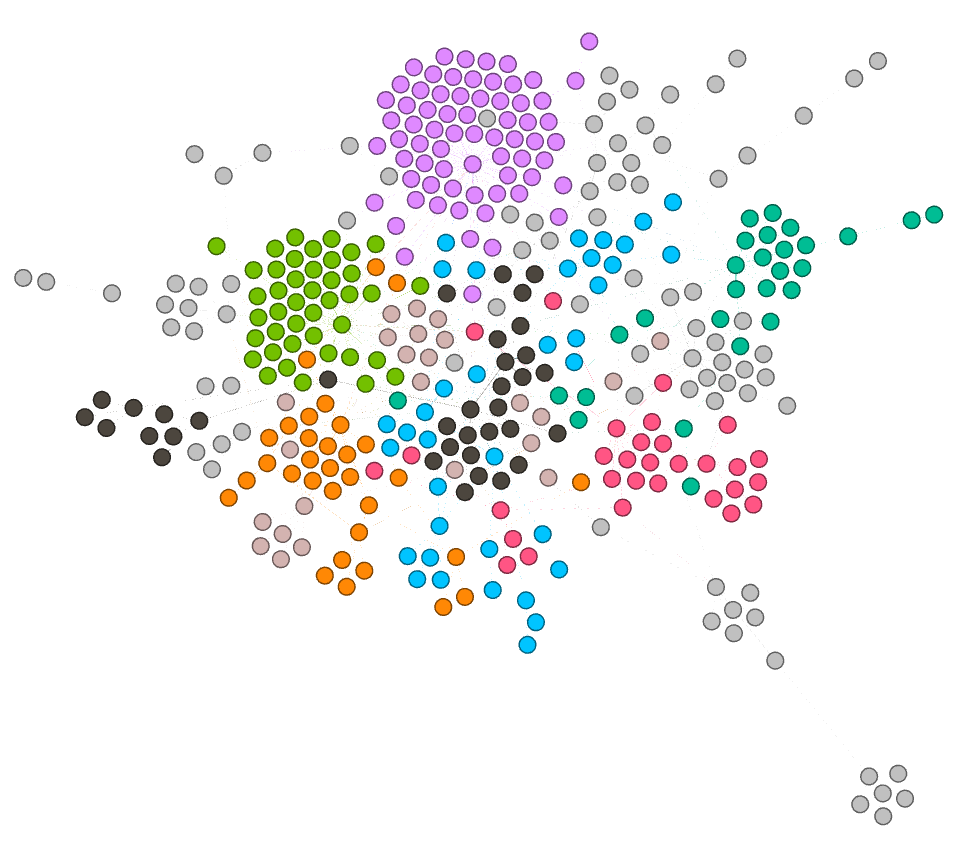
\includegraphics[width=0.80\textwidth]{fig/intro/disjoint_communities.png}
	\caption{Disjoint communities: vertices with unique labels.}
	\label{fig:disjoint_communities}
\end{figure}

Girvan and Newman (2003)\cite{Girvan2003} define a community as a subset of the set of network vertices that are densely connected to each other and have low connection density with the other network vertices not belonging to this subset. This is the definition of community widely accepted and used in the literature. Other nomenclatures analogous to the definition presented by Girvan and Newman are also found as, for example, modules \cite{Lancichinetti2009b}, \textit{clusters} \cite {Lancichinetti2011}, circles \cite{Leskovec2012}, which essentially keep the same concept, but they have specific characteristics that depend on the way the network is modeled and the objective proposed in each research.

%EX:
% modulos - partições do grafo 
% clusters - agrupamento - similaridade
% circulos - cliques de tamanho k

Girvan and Newman (2003)\cite{Girvan2003} further state that a community represents a partition of the original graph, such that each partition maximizes the internal density of the links and minimizes the density of the external links to the obtained parts. This view led to the study and proposition of measures and algorithms that aim to generate optimal partitions. Thus, many works in the literature address the problem of detecting communities as the problem of finding partitions of the network \cite{Dhumal2015, FORTUNATO201075, Lancichinetti2009b, Papadopoulos2012}. The Fig. \ref{fig:disjoint_communities} displays a graph with partitions, identified by vertices with equal colors. Each vertex is associated with only one partition. Each partition can be understood as a community, and the partition set represents a network with disjoint communities.

\begin{figure}[htb]
	\centering
	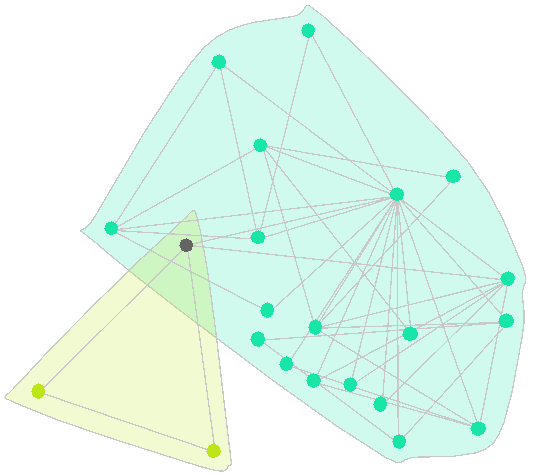
\includegraphics[width=0.80\textwidth]{fig/intro/overlap_communities.png}
	\caption{Overlapping communities: multi-label vertex highlighted.}
	\label{fig:overlap_communities}
\end{figure}

A feature of OSNs that can not be ignored during community detection is the fact that a vertex can be associated with several communities simultaneously \cite{Palla2005}. Communities on these networks do not exactly match different partitions. Social relationships between people often reveal this behavior, with the individual participating in communities defined by family structures, relationships among co-workers, friends of the school, etc. This phenomenon indicates that there are regions of overlap in the graph, with communities being formed by vertices that also belong to other communities. The Fig. \ref{fig:overlap_communities} provides the example of a vertex that is associated with two communities, revealing overlapping communities.

\subsection{Community Detection Algorithms}
\label{sec:comm_algorithms}

Since there are two understandings about how communities can be identified in OSNs, through partitions or overlapping, we will consider in this work the execution of algorithms that return results in both directions. We chose two algorithms that treat communities as partitions of the graph: RAK (initials of the algorithm authors) \cite{Raghavan2007} and INFOMAP (Maps of Information Flow) \cite{Rosvall2008}; and two algorithms that treat communities as overlapping regions in the graph: COPRA (Community Overlap Propagation Algorithm) \cite{Gregory2010} and OSLOM (order Statistics Local Optimization Method) \cite{Lancichinetti2011}. The following is a brief description of the operation of each of them. For more details we recommend reading the comparative analysis made by Fortunato and Lancichinetti \cite{Lancichinetti2009a}, Orman et al. \cite{Orman2012} and Xie et al. \cite{Xie2013}.

\subsubsection*{Disjoint Community Detection}
\label{subsec:disjoint_comm_detection}

The RAK algorithm acts from the Label Propagation concept. It is a simple algorithm that does not require any a priori information about the communities and also does not require the optimization of a predefined objective function, using only information from the network structure. Each vertex is initialized with a unique label and at each iteration of the algorithm the vertex adopts the label that most of its neighbors currently have. If more than one label is used by the same maximum number of neighbours, one of them is chosen randomly. In the end, the communities identified by the vertices that have the same labels. The time complexity of the algorithm is almost linear in the network size, which makes it computationally cheaper.

The algorithm INFOMAP describes random walks along the network encoding the path using two levels of identification, one identifier for the community and another for the vertex within the community, where vertices in different communities can have equal identifiers. The goal is to identify communities in order to minimize the size of the random path description. Intuitively, this is done by clustered together in clusters the vertices that often appear together in random paths. To identify the cluster, INFOMAP uses a greedy algorithm. Initially, each vertex is placed in its own community and communities are merged in order to reduce the expected size of the description of a random walk. Fortunato and Lancichinetti evaluated several algorithms and networks and concluded that INFOMAP was the most reliable of the evaluated methods \cite{Lancichinetti2009a}.


\subsubsection*{Overlap Community Detection}
\label{subsec:overlap_comm_detection}

%%%%%%%%%%%%%%%%%%%%%%%%%%%%%%%%%%%%%%%%%%%%%%%%%%%%%%%%
%%%%%%%%%%%%%%%%%%%%%%%%%%%%%%%%%%%%%%%%%%%%%%%%%%%%%%%%
The COPRA algorithm also uses the label propagation concept and is an extended version of the RAK algorithm for the detection of overlapping communities. A parameter $v$ controls the maximum number of communities a vertex can be associated with. In the tests performed by the authors of the algorithm, the best results for the community evaluation metrics were with the parameter $v$ set at 9, 10 or 11. COPRA also has the advantage of being fast in execution in larger and sparse networks because its complexity of time is essentially linear.

The OSLOM algorithm uses a method capable of differentiating the statistical significance of the real communities with the artificial communities that happen in random networks. Initially the algorithm randomly selects a vertex and adds it to a cluster. Then it analyzes each of the neighbors of this vertex and analyzes if the number of edges in the cluster is above what would be expected in a random network. Thus, at each step, significant vertices are added and insignificant vertices are removed of clusters. The results usually present significant numbers of outliers or singletons (communities formed by only one vertex). The worst case complexity in general is $O(n^2)$, while the exact complexity depends on the community structure of the underlying network under study.

\subsection{Community Quality Measures}
\label{sec:comm_quality}

The task of evaluating communities in OSNs is not trivial. It is not always possible to identify real communities so that some metrics can be used to compare detected communities and ground truth. This problem is known in the literature as ``lack of ground truth'' \cite{Zafarani2015}. The high values of clustering coefficients found in most real graphs indicate that the vertices in these graphs tend to form communities \cite{Girvan7821}, and therefore several metrics are employed from this approach to evaluate the quality of clusters formed and to circumvent the problem of lack of ground truth. In this work we will consider only community quality measures based on the evaluation without ground truth.

There have been a lot of studies about communities in Twitter \cite{McAuley:2012, Lim2012, Amitava:2012, Darmon2015, Amati2015, Mert2016, Achiam2016, Lim2016}, however, the great majority of them aim at discovering communities only in the graph formed by the follow relation. In this work, we also want to investigate the existence and quality of communities that can emerge on the other layers of a Twitter multilayer ego network. To this end, we present in this section some of the most used community quality measures in literature. For this purpose, lets consider a graph $G=(V,E)$, and a set of communities  $\mathcal{C}=\{C_1,\cdots C_{|\mathcal{C}|}\}$ in $G$ found by a given community detection algorithm. A community $C_i$ is a subgraph of $G$. We define $E_{C_i}^{in}$ as set of edges between vertices in $C_i$, $E_{C_i}^{out}$ as the set of edges  from the vertices  in community $C_i$ to the vertices outside $C_i$. Set $V_{C_i}$ is the set of vertices inside community $C_i$.



\subsubsection*{Newman{'}s Modularity}
\label{subsec:newman_modularity}
Newman{'}s modularity \cite{Newman2004b,Newman8577} is a measure of the quality of partitions imposed in a graph by a community detection algorithm.  Modularity measures how different the original graph is from a set of randomized graphs, in terms of the partitions existing in the original graph. For the given community partition of the graph $G$, modularity (Q) is given by \cite{Szymanski2013}:

\begin{equation}\label{eq:newmanModularity}
Q= \sum_{C_i \in \mathcal{C}} \left[ \frac{|E_{C_i}^{in}|}{|E|} - \left(  \frac{\alpha |E_{C_i}^{in}|+|E_{C_i}^{out}|}{\alpha |E|} \right) ^2 \right]
\end{equation}

where $\alpha$ is 1 for directed graphs and 2 for undirected ones. 

For weighted graphs, the definition of modularity is similar to the one corresponding to Eq. \ref{eq:newmanModularity}, however, $|E|$ in the equation is substituted with the sum of the weights of all edges in the graph,  $|E_{C_i}^{in}|$, is substituted with  the sum of the weights of all edges connecting  pairs of vertices inside $C_i$,  and $|E_{C_i}^{out}|$ is replaced by the sum of the weights of all edges connecting a vertex inside $C_i$ to a vertex outside $C_i$.


\subsubsection*{Internal Density}
\label{subsec:internal_density}
Communities usually have a great concentration of links among their internal vertices. Internal density is a local measure which evaluates the number of internal edges inside a community $C_i$ in $\mathcal{C}$ in relation to the total of possible edges inside $C_i$:
\begin{equation}\label{eq:intDensity}
D_{C_i} =\frac{\alpha|E_{C_i}^{in}|}{|V_{C_i}|(|V_{C_i}|-1)}, 
\end{equation} 
where  and $\alpha$ is 1 for directed graphs and 2 for undirected ones. The value of $D_{C_i}$ equals to one if $C_i$ is a clique. A global measure of internal density can be derived for graph $G$, by averaging the internal density values of all communities in $\mathcal{C}$.


\subsubsection*{Modularity-Density}
\label{subsec:modularity_density}
Community detection approaches  that try to maximize Neman{'}s modularity measure has two opposite yet concurrent problems. In
some cases,  a large community is  split into smaller communities. In other cases,  large communities  are formed by merging communities that are smaller than a certain threshold which depends on the total number of edges in the graph and on the degree of inter-connectivity between the communities \cite{Szymanski2013}. The latter problem is known as the resolution limit problem \cite{Fortunato36}. 

To solve both of the above mentioned problems, Chen, Nguyen and Szymanski \cite{Szymanski2013} proposed a measure termed  Modularity Density, as an alternative to modularity. 
Their measure modifies Newman{'}s modularity by introducing  two modifications in the original modularity formula: {\em Split Penalty} and {\em density}. Split penalty is the fraction of edges that connect vertices of different communities and solves the problem of favoring small communities. Density solves the resolution problem and is composed of two measures: internal density of each community (see Section \ref{subsec:internal_density}) and an the concept of internal density extended to consider a pair of communities. The Modularity-Density measure is defined as:

\begin{equation}\label{eq:modDensity}
\begin{array}{lll}
Q_{d} (G) =   \sideset{}{}\sum\limits_{C_i \in \mathcal{C}} \left[\frac{|E_{c_i}^{in}|}{|E|}D_{C_i} -    \left( \frac{\alpha |E_{C_i}^{in}| + |E_{C_i}^{out}|}{\alpha |E|}D_{C_i}\right)^2 
 - \sum\limits_{\substack{C_j \in \mathcal{C}\\C_j\neq C_i}} \frac{|E_{C_i,C_j}|}{\alpha|E|}D_{C_i,C_j}\right],\\
%&d_{C_i}= \frac{\alpha|E_{C_i}^{in}|}{V_{C_i}(|V_{C_i}|-1)}&,\\
%&d_{C_i,C_j} = \frac{|E_{C_i,C_j}|}{|V_{C_i}| |V_{C_j}|}&
\end{array}             
\end{equation} \vspace{4mm}
where $D_{C_i}$ is the internal density of community $C_i$ as defined in Eq. \ref{eq:intDensity}, and $D_{C_i,C_j}$ is  the pair-wise density between community $C_i$ and $C_j$ and is defined as:
$$ d_{C_i,C_j} = \frac{|E_{C_i,C_j}|}{|V_{C_i}| |V_{C_j}|}, $$
where $E_{C_i,C_j}$ is the set of edges from community $C_i$ to
community $C_j$. 


\subsubsection*{Conductance}
\label{subsec:conductance}
Conductance  measures the fraction of the
total number of edges that point outside the community:  
\begin{equation}
\label{eq:conductance}
\phi (C) =\frac{|E_{C_i}^{out}|}{2|E_{C_i}^{in}| +|E_{C_i}^{out}|}.
\end{equation}

As occurs with density, a global value of conductance can be obtained by averaging the conductance values over all communities. A smaller value of average conductance means better community quality. But the greatest the average conductance the more interconnected are the communities. 
\chapter{Related Works}
\label{cap:RW}


Social network analysis is a field in the study of sociology to enable methods, techniques and models to be developed to help researchers understand individuals' behavior and relationships. Graph theory has been widely used to aid in the identification and understanding of social network structures. Research conducted over the years has shown that social networks have peculiar structures that are not found in random graphs.

In 1969, Travers and Milgramm \cite{Travers:1967} conducted an experiment involving social relationships to evaluate the concept of the "small world" they had formulated years earlier. The results showed that the analyzed social network exhibits a high number of shortest paths, a structure that was found not only in other social networks but also in biological and technological networks by Watts and Strogatz (1998) \cite{Watts1998}. The fascination with these findings is revealed in the fact that this structure is not found in random graphs.

The organization of individuals in cohesive groups and the impact that the relationship can cause in the process of information diffusion was explored in 1973 by Granovetter \cite{Granovetter1973}, where the he concludes that the relationship is modeled in order to show strong bonds between individuals, forming communities, and weak ties that allow the interaction and diffusion of information between communities. Communities are also not found in random graphs.

Barabasi and Albert (1999) \cite{Barabasi509} conducted a study that presented a common characteristic found in several complex systems, among them some social networks, that is the fact of vertices connectivity following a scale-free power-law distribution. The authors state that this characteristic is a consequence of network expansion associated with the concept of "preferential connection", in which new vertices tend to connect with other vertices already well connected.

With the advent of the OSN, and consequently with the increasing amount of information present in these environments, researchers from different areas of knowledge were interested in the analysis of the structure of these networks. In 1997, Garton et al. \cite {Garton1997} developed a work to identify how online social networks could be analyzed and how virtual relationships would interfere with the functioning of social systems. The authors show that the analysis and description of relationships can be done with an ego approach - when the network is too large or difficult to define - as well as through a global analysis - when the entire network is available. Some characteristics of the OSN that should be carefully analyzed, according to the authors, are: size (hence the heterogeneity of individuals), structural position of individuals, similarity of behavior of individuals and formation of groups. The authors also report that social networks need to be explored from a multilayered view, but so far there have been few studies that explore this last item.

In the work of Ahn et al. (2007) \cite{Ahn2007}, the authors compare the structure of three OSNs: Cyworld, MySpace and Orkut. The properties analyzed were the distribution of degrees, grouping properties, correlation of degrees and evolution over time. The only complete OSNs was Cyworld, and for the other networks small samples were used. The results for MySpace and Orkut have been very close, while the Cyworld network differs from the others and seems to achieve a stabilization over time. The authors also showed that the analyzed OSNs differ from real-life social networks in the analyzed aspects.

Mislove et al (2007) \cite{Mislove2007} also analyzed the structure of different OSNs: Flickr, YouTube, LiveJournal, and Orkut. The authors concluded that the analyzed OSN have the following properties: scale-free power-law degree distribution and small-world phenomenon. the authors also report that node input degrees tend to approach output degrees and that networks have core of vertices with high densely connected degrees that attach to small groups of vertices with low degrees but strongly grouped. The same properties also reported in the work of Fu et al. (2008) \cite{Fu2008}, who analyzed a blog and a Chinese social network.

So far we have presented only works that analyze OSN structures using only a specific type of interaction. Current OSNs allow their users to use various forms of interaction, which may have different meanings and intensities, characterizing them as multilayer networks. Our proposal is to analyze structures present in the various layers of Twitter's ego networks. The ego approach will be used taking into account the advantages presented in the Introduction of the dissertation. In section \ref{sec:ego_net_analysis} we present some of the main works that analyze the structural properties of ego networks, and in section \ref{sec:multilayer_net_analysis} we present some of the main works that analyze the structural properties of multilayer networks.

%%%%%%%%%%%%%%%%%%%%%%%%%%%%%%%%%%%%%%%%%%%%%%%%%%%%%%%%
%%%%%%%%%%%%%%%%%%%%%%%%%%%%%%%%%%%%%%%%%%%%%%%%%%%%%%%%


\section{Structural Analysis of Ego Network}
\label{sec:ego_net_analysis}

The comparison between ego network properties in OSN and social networks in the real world, or offline networks, has been widely investigated. Once researchers are able to compare these two environments, the analysis of ego networks can be performed more efficiently, because in the OSN it is much more practical to collect the relationship data. As most researches have shown several similarities between the two environments as in \cite{Gala2012,Arnaboldi:2012,Arnaboldi:2013,Arnaboldi:2013a,Arnaboldi:2016,Arnaboldi:2017a,ARNABOLDI2017}, the OSNs become essential tools for understanding human behavior. However, as we can observe in the following work description, the vast majority of them consider only the comparison of structures present in OSN with well-known patterns in the study of offline social networks, and that a great amount of information may be being discarded. We conjecture that the use of appropriate measures and modeling for graph analysis can shed light on patterns not yet explored in the OSN ego networks.

In Arnaboldi et al. (2013) \cite{Arnaboldi:2013}, analyzes show that Twitter presents social structures qualitatively similar to those found by the authors themselves on Facebook and by Dunbar in ego offline networks. The modeling of Twitter's ego networks was accomplished by aggregating the follow, retweet, mention, and replies interactions indistinctly. The comparison was made by identifying similarity between the pattern found in offline ego networks known as Dunbar circles, and the Twitter's ego networks that they modeled. The results suggest that the structure of a Twitter's ego network is controlled by the same cognitive properties of the human brain operating in offline ego networks.

The behavior of the users in different OSN was studied in Arnaboldi et al. (2013a) \cite{Arnaboldi:2013a}. Here the authors also perform a comparison between ego networks in OSN and offline ego networks in the sense of analyzing the dynamic processes of ego networks and personal social relations on Twitter. The authors suggest that human behavior on Twitter differs significantly from other social networks studied in the literature in different fields of research. Twitter ego networks are generally smaller and have a high percentage of weak and dynamic links, which culminates in a difficulty in determining that there is a hypothetical decline in Twitter usage, unlike in other OSNs.

Already in Arnaboldi et al. (2016) \cite{Arnaboldi:2016} and Arnaboldi et al. (2017) \cite{ARNABOLDI2017}, the authors analyze the behavior of users in online and offline ego networks to identify common patterns their relationship with the process of information diffusion. The authors state that this understanding can be useful in creating new services for the Internet of the Future, such as highly personalized ads, tailored to the needs and characteristics of each user. The results point to the similarity in the behavior of online and offline ego network users during the process of information diffusion.

In Arnaboldi et al. (2017a) \cite{Arnaboldi:2017a}, the authors state that the evolution of the bonds between ego and alters is very dynamic, suggesting that they are not entirely used for social interaction, but for public signposting and self-promotion.

In the works described so far that compare the structures found in ego networks in the OSN and ego networks in offline social networks, the authors model star ego networks, that is, they considered only the relationship between ego and alter, ignoring the alters-alters edges. Another important point is that they also disregard the meaning of each interaction, forming an aggregate network, not evaluating the importance of each interaction in the aggregate network formation process. Our proposal differs from these works precisely by modeling ego networks considering the meaning and importance of each type of interaction and considering the alters-alters edges.

The analysis of ego networks usually happens when you do not have enough data to model the entire network. However, the results obtained in analyzes of ego networks show that they may be different from the results obtained when the entire network is analyzed. This fact shows that an ego network analysis should be considered only when the intent is to actually observer user behaviors in a local approach, otherwise the results may be distorted.

Gupta et al. (2015) \cite{Gupta2015} analyzed different OSNs (social, co-authoring, communication and hybrid) and show that the structural properties of ego networks are different from the entire network. For this the authors analyzed the distribution of degrees, degree of assortativity and clustering coefficient of ego networks derived from each considered OSN and compared with the same metrics calculated across the network. These results help to better understand and correct the biases resulting from insufficient local information in the OSNs, thus allowing an effective analysis of social behaviors.

The social networks analyzed by Gupta et al. were Facebook and Orkut, and the modeling of ego networks is accomplished through the explicit friendship relationship between users on these OSN. Our local approach takes into account the results presented by Gupta et al. and in our analysis we are focused in studying the characteristics of an individual and his/her social environment as a way to detect repetitions of patterns at different points in the whole network and to open the way for works that improve the offer of personalized services.

In the work of \cite{Muhammad2015}, the authors characterized structural patterns of alters in nine publicly available spatial-temporal, collaboration and social ego networking datasets. Using graph mining techniques, the authors extracted features that can be classified according to centrality, efficiency, transitivity, and actor-based, and applied unsupervised clustering techniques to identify and categorize eight ego neighbors' clustering patterns still in connected structures, dense structures, informative ego and less dense structures. The authors also analyzed the behavior of the alters by comparing the patterns found by the same set of users in three different OSNs. Here the authors only make a structural characterization of ego networks, not an analysis as we propose.

In the work of Achiam et al. (2016) \cite{Achiam2016}, the authors analyzed the ego network structure of followers of some Twitter profiles associated with companies, ie using the followee interaction. They show that the distribution of the ego network does not follow a power-law, that is, it is not scale-free and is not random. From then on they present a model for capturing the dynamics of these ego networks specifically focused on companies and the type of relationship derived from the followee interaction. Here the authors modeled and analyzed specific ego networks through a single type of interaction. We are interested to find out if there are common patterns in ego-modeled networks from different points of Twitter. For this we analyze several types of interaction between the vertices of several ego networks.
%%%%%%%%%%%%%%%%%%%%%%%%%%%%%%%%%%%%%%%%%%%%%%%%%%%%%%%%
%%%%%%%%%%%%%%%%%%%%%%%%%%%%%%%%%%%%%%%%%%%%%%%%%%%%%%%%

Among the papers that seek to analyze structural patterns present in Twitter ego networks, there are those who dedicate themselves to detect communities \cite{McAuley:2012,Leskovec2012,Dykstra2014,Epasto2015}. Girvan and Newman (2003) \cite{Girvan2003} define a community as a subset of the set of network vertices that are densely connected to each other and have low connection density with the other network vertices not belonging to this subset. This is the widely used definition, although there are other models and other nomenclatures \cite{Lancichinetti2009b, Lancichinetti2011, Leskovec2012}.

Soundarajan and Hopcroft (2015) \cite{Soundarajan2015} show that detecting small groups of strongly connected nodes, according to a local association criterion, that is, in an ego approach, and the subsequent expansion of these small groups, produce communities more accurate than methods that only evaluate the structure of the entire network. This finding justifies the number of works that are dedicated to detecting communities in ego networks and to understand their structure and evolution.

McAuley and Leskovec (2012) \cite{McAuley:2012,Leskovec2012} address the problem of detecting communities by detecting what the authors consider as social circles of OSN users. The authors collected a set of 1000 ego networks from Twitter's follow interaction, each with a maximum of 4964 alters, plus some other Facebook and Google+ ego networks, all with manually labeled ground truth. The detection model combines the ego network structure and characteristics of the alters' profiles to group them into communities from the similarity between them. Among the characteristics used in the process of community formation, the authors do not consider the different types of interaction between the ego and the alters. 

The proposed model by McAuley and Leskovec is able to identify overlapping and hierarchical communities and it was elaborated in order to identify different similarity patterns for each community, which fits very nicely to the problem of identification of ego network communities, and would be impracticable in larger networks with thousands of us. The results show that the combination of the network structure with characteristics of the user profiles used by the proposed model was able to accurately identify the communities in a diverse set of data from Facebook, Google+ and Twitter. The application suggestion is to create a tool that uses the proposed template for automatic creation of Twitter lists.

For Dykstra and Lijffijt (2014) \cite{Dykstra2014} the problem of detecting communities in ego networks can be realized by predicting communities from a collection of duly labeled and collected data about other user communities. They propose the use of a database of lists collected from various users on Twitter to predict which lists fit best according to the structure of a particular user's ego network. The authors collected information on Twitter follow and follower interactions to model a total of 24 ego networks used in the experiment.

In the work of Epasto et al. (2015) \cite{Epasto2015} authors use Twitter's follow interaction to model ego networks and detect communities in those networks. The purpose of the paper is to identify similar alters that co-occur in different communities for recommendation of friendship between them within the OSN. Again we note that other types of user interaction are ignored at the expense of the explicit friendship relationship.

In the described works that detect communities in ego networks in OSN, we observe that the ego networks modeling is done only based on static information, such as the explicit friendship relationship defined in each OSN and information extracted from the users profile. Note that there is a very large amount of information present in other types of interaction, mainly because they are considered dynamic and performed with different intensities, which are simply ignored. The modeling proposed in this dissertation can be used as a way to verify if other types of information derived from dynamic interactions can also produce accurate communities.

%Não se encaixa no contexto de trabalhos correlatos...
%Papers that attempt to detect communities (lists) on Twitter ego networks, whether for the recommendation of lists or friends, have often used just the follow interaction to model the networks. We conjecture that the use of another type of interaction will be able to produce similar or even better results, since lists can be created as a way for the ego to receive content from a specific group of users that are not necessarily part of the friendship circle of the ego, or that simply the ego did not want to be identified as a follower of those alters. In this sense, the structural analysis of ego networks modeled based on information from other types of user interactions can change the perspective of the existing works in the literature that use only one type of interaction as the basis for the detection of communities in OSN.

% - Não trabalha análise estrutural - apresenta uma ferramenta para identificar padrões em grafos.
%In the work of Moustafa et al. (2012) \cite{Moustafa:2012} the authors present a new interface in the ego network analysis process, which may facilitate the process of finding patterns present in graphs, proposing a declarative language based on SQL. The queries made in this language should allow the display of patterns present in the relationships between the elements of an ego network, such as the node degree or its local grouping coefficient, for example. The data retrieved by the query can still be used in later analysis. The goal is to compare the graph under analysis with known structures that are stored in a database by performing a query through the SQL language. The authors also emphasize that this model can be useful in many domains in the analysis of social networks, including identification of opinion leaders, classification of nodes, prediction of links and identification of functions.


\section{Structural Analysis of Multilayer Network}
\label{sec:multilayer_net_analysis}

The analysis of multilayer networks passes through the understanding of the structure of the networks observing different relationships existing between the vertices. In the literature there are works that present a study and, generally, the comparison between the structures of each layer \cite{Wilson2009,Kwak:2010,Szell2010,Cardilo2013,Nicosia2015,Amati2015,Darmon2015,Omodei2015,DeArruda2016,Hong2016}, and works that analyze a single network structure formed by the aggregation of all the layers \cite{Boccaletti2014,Azaza2015,DeDomenico2015,Kuncheva2015,Hajibagheri2016,Azaza2016,Kleineberg2016,Vahedian:2017,Ding2017}. Here we present a brief description of some works that make a comparative analysis between structures found in different layers of the same multilayer network. The results of these works indicate the need to evaluate the formation process of the layers and the nature of the links between the elements of the network, according to what we are proposing in this dissertation.

In Wilson et al. (2009) \cite{Wilson2009}, the authors collected data from Facebook and modeled two networks, one with static reciprocal network friendship interaction and another with dynamics interactions between users. The comparison between these two networks showed that the dynamics interaction network presents larger diameters, lower clustering coefficients, and higher assortativity. The authors also report that only a small number of users maintain interaction activities, and that the number of interactions is limited by constraints, such as observation time, which calls into question the evaluation of OSNs only with the modeling of interactions dynamics. Even so, they strongly suggest that OSNs based applications are also designed with graphs of dynamic interactions and not only with static interactions.

Kwak et al. \cite{Kwak:2010} collect the whole network of Twitter and did an analysis of the topological characteristics through the type of interaction "follow" and the process of information diffusion. The main results of the analysis show that degree distribution did not follow a power law, diameter and reciprocity were low, countering what is expected in a social network in the real world. In another analysis the authors showed that the rankings of number of followers and number of retweets were different. Another important feature was the fact that a tweet that is retried reaches an average of 1,000 users, regardless of the number of followers of the original tweet author. This fact shows the power process of disseminating information on Twitter and the importance of retweet interaction.

According to Szell et al. (2010) \cite{Szell2010} the multidimensional nature of many social networks has been ignored, with the researchers giving emphasis to the study of only the topology of these networks, mainly due to the lack of available data. In their work the authors analyzed a complete multilayer social network, formed by the players of an online multiplayer game. By analyzing the network layers independently they found that they differ in relation to reciprocity, clustering coefficient and degree distribution, indicating that the combination of layers in a multilayer network may cause a poor representation of the system, hiding patterns presented in each layer.

%\cite{Szell2010}
%In their work the authors analyzed a complete multilayer social network, formed by the players of an online multiplayer game. Six types of interactions were modeled as layers of this multilayer network and classified into positive interactions (friendship, communication and trade) and negative interactions (enmity, aggression and punishment). The comparison between the layers showed that the negative interactions differ from the positive interactions by having lower reciprocity, weak clustering and long tail degree distribution. The authors further evaluated how the interdependence of different types of layers interferes determines the organization of the system. By studying the correlation and the overlap between different types of interactions, the results suggest that users play different roles in different layers.

In the work of Cardillo et al. (2012) \cite{Cardilo2013} the authors analyzed the structural properties of a multilayer network from flight data between airports in Europe. Flights operated by each airline represent one layer in the multilayer network. The results obtained by them indicate that topological properties of the whole system are not found in isolated layers, emphasizing the importance of evaluating the structural characteristics of each layer to understand the dynamic processes that occur in the aggregate network. The measures used in the topological analysis were the distribution of degree, average path lenght, coefficient of clustering, the size of the giant component and the Rich-club coefficient\footnote{Measures the tendency of highly connected nodes, i.e. the hubs, to be connected among themselves.}. Similar results were found by Hong et al. (2016) \cite{Hong2016} in a multilayer representation of the Chinese air transportation network (ATMN).

%In the work of Cardillo et al. (2012) \cite{Cardilo2013} authors question whether previous work evaluating structural features of complex networks is characterizing the unique layers. To answer this question they have modeled and analyzed the structural properties of a multilayer network from flight data between airports in Europe. Flights operated by each airline represent one layer in the multilayer network. The results obtained by them indicate that topological properties of the whole system are not found in isolated layers, but are representations of an emergent phenomenon closely related to the multilayer character of the system. The measures used in the topological analysis were the distribution of degree, average path lenght, coefficient of clustering, the size of the giant component and the Rich-club coefficient\footnote{Measures the tendency of highly connected nodes, i.e. the hubs, to be connected among themselves.}. In experiments where some layers are merged, according to structural similarity, as low cost airlines compared to large companies, it leads to the emergence of qualitatively different aggregate networks. And the authors emphasize the importance of evaluating the structural characteristics of each layer to understand the dynamic processes that occur in the aggregate network.

In \cite{Omodei2015} interactions between Twitter users were analyzed during exceptional events that related to politics, culture or science. For each event, \emph{retweets}, \emph{mentions} and \emph{reply} data were collected and a multilayer network constructed according to these activities. An analysis of each layer showed that between them there are significant differences between some structural properties, such as degree distribution and clustering coefficient. These results obtained in specific networks arouse the interest in carrying out a deeper analysis, such as the one we are proposing.

The detection of communities in OSN also began to be studied in multilayers networks. In \cite{Darmon2015} the authors performed the process of detecting communities on Twitter according to the type of action performed by the users. The generated communities were classified in: based on the relationship, the activity and the interactions between the users. The results showed that there are situations where the structures of these communities are similar, as there are also situations where the structures are completely different. Here the authors still mixed some interactions to model the three classes of networks studied. We intend to perform an analysis of the structure of each type of interaction in isolation.

Nicosia and Latora (2015) \cite{Nicosia2015} conducted a comparative study between layers of the same multilayer network to verify correlation between node activities and their degrees. The data set used is composed of real-world biological, technological, and social systems and spanning a wide range of sizes. The results show that real-world networks exhibit non-trivial multilayer correlations, which indicates that a representation of an aggregate network formed from the sum of its layers hides specific patterns of each layer. The authors caution that the role played by each layer's patterns may be responsible for completely new, unobservable physical phenomena in single-layer projections. Similar results were found by De Arruda et al. (2015) \cite{DeArruda2016} in a multilayer representation of an airport transport network.

A comparative structural analysis between layers modeled according to different types of interaction in a multilayer Twitter network was performed by Amati et al. (2015) \cite{Amati2015}. The dataset used is formed by data collected from users who are part of the public administration activities of Italy and its followers, with profiles in Italian language. From the metrics like degree distributions, connected components, path length distributions and clustering coefficients, the authors show the layers that correspond to the interaction of the mention type and retweets has higher information spreadind, compared to the layer of the follow interaction. Our work differs from Amati's research by performing a comparative structural analysis on a large number of ego networks.

Most of the studies on how to identify patterns in online social networks do not present conclusive results on the best way to treat the multilayer nature of these networks. We also did not find work evaluating the properties of multilayers networks using an egocentric approach to Twitter users. In this work we present results for metrics that evaluate the structural properties of each layer in a set of Twitter ego-networks, which is convenient for detecting repetitions of patterns or tendencies in the whole network.


%%%%%%%%%%%%%%%%%%%%%%%%%%%%%%%%%%%%%%%%%%%%%%%%%
% Conteúdo do Artigo... analisar para ver se encaixa em redes agregadas.
%%%%
%The prediction of Twitter links presented in \cite{Hajibagheri2016} shows that a more accurate result can be found by considering the properties of a multiplex network, rather than analyzing each layer in isolation.

%The combination of \emph{retweet}, \emph{reply}, \emph{reintroduce}, and \emph{read} actions among Twitter users forms a multilayer network that is explored in \cite{Zhaoyun2013}. The authors perform a sequence of random walks in the combined network to determine the influence of users, achieving convergence after four rounds.

%Detecting influential users on Twitter is also the purpose of the work \cite{Azaza2015} and \cite{Azaza2016}. The authors collect data on the European Parliament elections in 2014 and build a multilayer network combining the weight of user interactions in each layer: \emph{retweets}, \emph{mentions} and \emph{reply}. A general measure that quantifies the combination of different interactions is used to determine the degree of influence of a user.

%%\chapter{Analysis of Twitter Multilayer Ego Networks}
%\label{cap:Background}

%%%%%%%%%%%%%%%%%%%%%%%%%%%%%%%%%%%%%%%%%%%%%%%%%%%%%%%%
%%%%%%%%%%%%%%%%%%%%%%%%%%%%%%%%%%%%%%%%%%%%%%%%%%%%%%%%

\chapter{Twitter Multilayer Ego Networks}
\label{cap:ExpSetup}

In this chapter we define the Twitter multilayer ego network model used in this dissertation and we describe how we collect the dataset used in the experiments. In section \ref{sec:MEN} we have the formal definition of Twitter multilayer ego networks. Section \ref{sec:dataset} describes the procedures for collecting the dataset. In sections \ref{sec:dataset_follow_network} and \ref{sec:dataset_retweets_network} are the formal definitions of how we model the layers of the multilayer ego networks from the collected data.

%%%%%%%%%%%%%%%%%%%%%%%%%%%%%%%%%%%%%%%%%%%%%%%%%%%%%%%%
%%%%%%%%%%%%%%%%%%%%%%%%%%%%%%%%%%%%%%%%%%%%%%%%%%%%%%%%


\section{Definition of Twitter Multilayer Ego Networks}
\label{sec:MEN}
Given a Twitter user $e$, to whom we refer  as {\em ego}, we define the {\em multilayer ego network} $\mathcal{G}_e$ of $e$ 
as a  family of directed graphs  $\mathcal{G}_e=\{G_e^{\alpha};  \alpha \; \in\{1, \cdots m\} \}$. Each  graph  $G_e^{\alpha}$ is  a {\em layer} of $\mathcal{G}_e$ and is associated to a  Twitter interaction  of type $\alpha$.  $G_e^{\alpha}$ is defined as the pair $G_e^\alpha = (\{e\} \cup A_e^{\alpha}, E_e^{\alpha})$.  
Set $\{e\} \cup A^\alpha_e$ is the vertex set of graph $G_e^\alpha$.  $A^{\alpha}$ is the set of  all Twitter users that $e$ has interacted with at least once by interaction of  type $\alpha$. We refer to $A_e^{\alpha}$ as the  {\em alter set of $e$ regarding interaction of type} $\alpha$, or simply as the {\em alter set of} $e$ when the type of interaction is implicit in the context. Set $E_e^{\alpha} =  \{(v_i,v_j) | v_i,v_j \in \{e\} \cup A_e^\alpha: v_i \neq v_j\}$ is the set of directed edges or ordered pairs of the form $(v_i,v_j)$, meaning that user $v_i$ has interacted with user $v_j$ at least once by the interaction of type $\alpha$. 


According to the above definition, a multilayer ego network for a user $e$ has the following characteristics: a) a user $a$ is an alter of $e$ in layer $\alpha$ ($a \in A^{\alpha}_e$), only if $e$ interacted directly with $a$ by an $\alpha$ interaction, i.e., an edge $(e,a)$
must exists in $E_e^{\alpha}$; b) there may  be an edge  $(a_1,a_2)$ (an {\em alter-alter} edge) in $E_e^{\alpha}$ as long as $e$ has interacted with both $a_1$ and $a_2$ by interactions of type $\alpha$ (i.e., $a_1,a_2 \in A_e^{\alpha}$) and $a_1$  has also interacted with  $a_2$ by an interaction of type $\alpha$; c) there may be an edge $(a_1,e)$ (an {\em alter-ego} edge) in $E_e^{\alpha}$ which implies that the  ego $e$ and the alter $a_1$ have both interacted with each other by interaction $\alpha$; d) a same user $a$ may be an alter in as many layers of an ego $e$, as the number of distinct interaction types $e$ has used to interact with $a$. 
 
%Notice that according to the above definition, a multilayer ego-network for a user $e$ has the following characteristics:

%\begin{itemize}
%\item The set of vertices forming a layer is composed only by the ego $e$ herself  and  by the one-step neighbors of $e$ in Twitter according to interaction $\alpha$. That is, we include as the alter set of $e$ only those Twitter users
%that the ego has interacted directly with  by interaction of type $\alpha$. 
%\item An edge $(a_1,a_2)$ such that $a_1 \neq e$ and $a_2\neq e$ pertains to    $E_e^{\alpha}$ if only the pair of edges $(e, a_1)$ and $(e, a_2)$   also pertain  to  $E_e^{\alpha}$. In other words, edge $(a_1,a_2)$ means that $a_1$ has also interacted with $a_2$ by means of interaction of type $\alpha$,  but this edge exists in $E_e^{\alpha}$ only if both vertices are alters of $e$.
%\item   A same alter $a_1$ may take part in more than one layer of an ego $e$. For instance, if $e$ interacted with $a_1$ by means of interactions of types $\alpha_1$ and $\alpha_2$, we have that $a_1$ takes part in both alter set $A_e^{\alpha_1}$ of layer $G_e^{\alpha_1}$ and in alter set $A_e^{\alpha_2}$ of layer $G_e^{\alpha_2}$ .
%\end{itemize}
One may think of  a great number of layers for a multilayer ego network derived from the Twitter OSN, by considering different types of  interactions between pairs of Twitter users. However, in this work, we are interested  in interaction types derived from the four most common  operations  in Twitter:   {\em follow}, {\em retweet}, {\em like} and {\em mention}. The follow operation allows a user $e$ to inform Twitter that $e$ wants  to follow a specific user $a$. This means that $e$ will start receiving in her timeline every tweet authored by or propagated by $a$ via a retweet operation. The mention operation allows a  user $e$ to send a tweet directly to another user $a$. In this case, the tweet works like a message sent by $e$ to $a$. The retweet operation is applied by a user $e$ to a tweet $t$. The effect of the retweet is that $t$ is propagated to all users that follow $e$.  Finally, the like operation is also applied by a user $e$ to a tweet $t$ and simply marks $t$ as a tweet that $e$ liked to receive. 
 
The above four operations in Twitter imply in interactions among users. The follow and the mention are  operations one user perform over another since a user  uses these operations to, respectively,  establish  a communication channel with  or  send a message to  another user. The retweet and like operations are, on the contrary,  operations over a tweet and not directly between users. However, both represent the fact that a user found interesting a piece of text (tweet) authored by another user. In this sense, both are considered  interactions between the receiver and the  writer of the tweet. Thus, from this point on, we refer to follow, mention, like and retweet as  direct interactions between two Twitter users. 
 
\begin{figure}[htb]
	\centering
	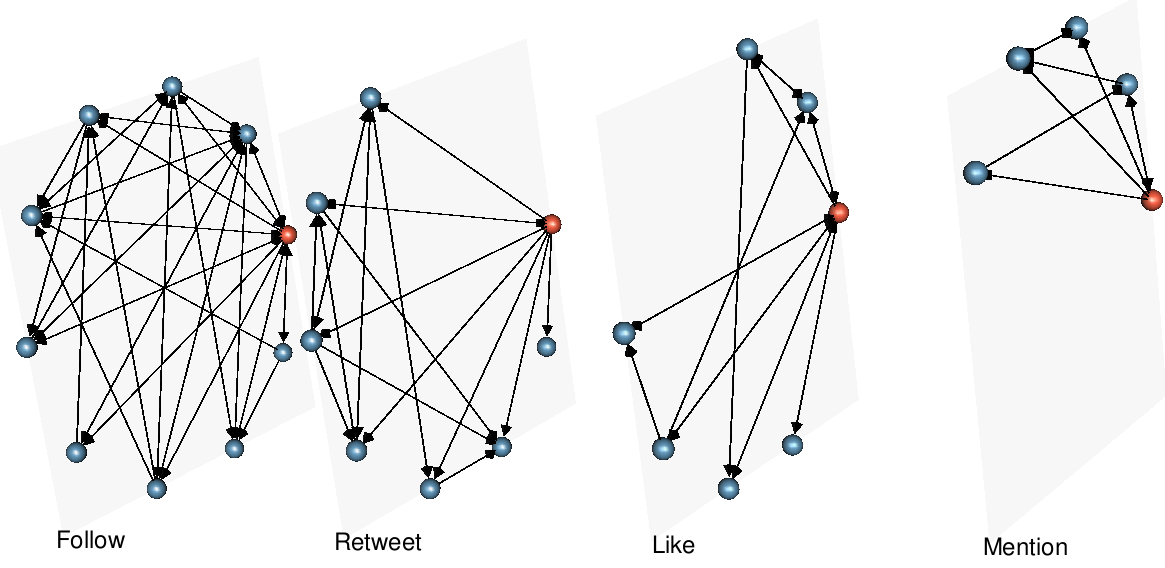
\includegraphics[width=1\textwidth]{fig/multilayer/layers_oneLine.png}
	\caption{Example of a multilayer ego network in Twitter. Ego {\em e} highlighted in red.}
	\label{fig:ex_multilayer}
\end{figure}
 
In this way, for a user $e$,  we can derive four different interaction layers or graphs in Twitter: $G_e^f$, $G_e^m$, $G_e^r$ and  $G_e^l$, where the letter in the superscript of each graph represents   the initial of the corresponding interaction. Each of these graphs are built as described in the first paragraph of this section, by substituting $\alpha$ for {\em follow, mention, retweet} and {\em like} interactions, respectively. Together these four graphs form a multilayer ego network of user $e$, represented as $\mathcal{G}_e=\{G_e^f, G_e^m, G_e^r, G_e^l \}$. Fig. \ref{fig:ex_multilayer} presents an hypothetical example of a multilayer ego network for an ego $e$. 




\section{Dataset} \label{sec:dataset}

We started collecting data with an initial set of users formed by the 100 users who were the last to write a tweet related to any of the ten Twitter trend topics in January, 14, 2017. We adopted a {\em snowball}\footnote{Sampling technique where the data set is formed from initial elements that meet the search criteria, called seeds, and the set grows from these.} strategy to derive a large set of users from which we selected our final sample of users (egos) for whom we obtained the multilayer ego networks.  

Since the layers of the ego networks correspond to interactions in Twitter, we opt to not use Twitter interactions to drive the harvest of users in order to avoid  bias towards any layer type. Thus, we opted to use Twitter lists in the process of expanding the set of users. Also, the choice of using list during the process of obtaining the egos was taken because we wanted to investigated if lists could be uses as ground truth for community detection in each layer for a given ego, as we explain in \ref{sec:QuestionTwitterLists}. 

We first collected a set of {\em possible egos} $P$. During the harvesting process to obtain $P$, we adopted the following expansion criterion: {\em a user would be included in $P$  only if she has subscribed or owned at least one Twitter list with at least five members}. Only eleven of the 100 initial users satisfied this criterion and they were initially inserted in set $P$. 
Starting from the seed set in $P$ our harvest method adopted a breadth-first search where it picked one user $u$ among users already in $P$ and collected the other users in the lists where $u$ was involved. Only the users in the lists that satisfied the expansion criterion defined above were inserted in $P$,  and the process continued by picking another user in $P$ not considered yet. We stopped the harvest process when $P$ contained  a total of 10,000  possible egos.

Only 3,983 of the 10,000 users had public data and they formed the final collected set. From this set, we randomly chose 500 users to form our final ego set $\mathcal{E}$. We limited the number of egos to 500 due to the cost of obtaining, modeling and analyzing all layers for more egos. 

Once the set of egos $\mathcal{E}$ has been collected, we obtained for each ego $e \in \mathcal{E}$ the four layers: $G_e^{f}$, $G_e^{r}$,  $G_e^{l}$ and $G_e^{m}$. Both the ego set $\mathcal{E}$ and the graphs composing the multilayer ego network of users in $\mathcal{E}$ were collected using the Twitter REST API\footnote{https://developer.twitter.com/en/docs/developer-utilities/usage-api/overview.html}. 

The four layers for each ego in $\mathcal{E}$ are defined in \ref{sec:MEN}, however there are some limitations in Twitter API and also some characteristics of Twitter that imposed some restrictions on the number of alters and, consequently, on the number of edges we used to form each layer. In what follows we comment on the difficulties found in collecting alters  and the resulting limitations in the number o alters in each layer.


%%%%%%%%%%%%%%%%%%%%%%%%%%%%%%%%%%%%%%%%%%%%%%%%%%%%%%%%
%%%%%%%%%%%%%%%%%%%%%%%%%%%%%%%%%%%%%%%%%%%%%%%%%%%%%%%%


\section{The \texorpdfstring{$G_e^f$}{Gef} Layer}
%\section{The $G_e^f$ Layer}
\label{sec:dataset_follow_network}

For almost all egos $e$ in  $\mathcal{E}$ we collected all the users that $e$ follows in Twitter (i.e $e$'s followees) to form the alter set $A_e^f$ of $e$.  However, for approximately 15\% of the egos in $\mathcal{E}$, we collected up to 5,000 of their followees. We imposed this limit on the number of followees collected because it would be prohibitive to obtain the whole follow layer for these egos. This is  because the Twitter API limits the number of requests to collect the followees to only 15 requests every 15 minutes and for each followee we would also need to collect its followees in oder to obtain the edges of the follow layer for each ego. Thus the time to collect the complete follow layer would be huge for those egos with more the 5,000 followees.

Once we collected the alter set $A_e^f$ for an ego $e$, we obtained de edge set $E_e^f$ for $G_e^f$. We started by  creating an edge from $e$ to each of her alters. Next, for each alter in $A_e^f$ we obtained its followees and for every followee $b$ of $a$, such that $b \in  \{e\} \cap A_e^f$ we inserted  a direct edge $(a,b)$ in $E_e^f$. 
 


%Once this limitation happens only to few egos in our 500 ego set it is not an important burden in our analysis. For each alter we also collected their followees only to determine the links among alters and $e$.


%%%%%%%%%%%%%%%%%%%%%%%%%%%%%%%%%%%%%%%%%%%%%%%%%%%%%%%%
%%%%%%%%%%%%%%%%%%%%%%%%%%%%%%%%%%%%%%%%%%%%%%%%%%%%%%%%


\section{The \texorpdfstring{$G_e^r$}{Ger}, \texorpdfstring{$G_e^l$}{Gel} and \texorpdfstring{$G_e^m$}{Gem} Layers}
%\section{The $G_e^r$, $G_e^l$  an $G_e^m$ Layers}
\label{sec:dataset_retweets_network}
The Twitter API does not allow for direct requesting the retweets, likes or mentions made by  a user (ego) $e$. It is necessary to collect $e$'s timeline and to inspect all tweets in it to determine which of them were retweeted, liked  or a mention by  $e$. The alter sets $A_e^r$ and $A_e^l$ are composed of the authors of the tweets rewetted and liked by $e$, respectively. The alter set $A_e^m$ is composed of users to whom $e$ sent a mention-tweet.

The timeline of $e$ must be inspected in order to derive these alter sets. However, the Twitter API limits the number of tweets that can be collected in a user timeline to 3,200 tweets.  Thus, the sizes of  the alter sets $A_e^r$, $A_e^l$ and $A_e^m$ are limited to 3,200 users. In practice,  not all of the tweets in a timeline are rewetted, liked or are mentions, thus the sizes of these alters sets tend to have much less than 3,200 alters.

After collecting  the alter set for the four layers, we obtained the edge set for each of them. In each layer, we first create edges between the ego $e$ and each of her alters. Next, for each alter $a$ in a layer, we access $a$'s timeline and for each tweet that $a$ interacted with, we obtain the user $b$  which is the author of the tweet or is mentioned in the tweet. If $b \in \{e\}\cap A_e^f$, we create and edge from $a$ to $b$ in the edge set of the corresponding layer.

%The first line of Tables \ref{tab:numVertices} and \ref{tab:numEdges}  show information about the number of vertices and the number of edges in the 500 $G_e^f$ obtained. 

\chapter{Results}
\label{cap:Results}

Many samples collected by different studies have shown that Twitter is a scale-free\cite{Kwak:2010,Borondo:2016}, small-world\cite{Java:2007} and have community structure\cite{Java:2007,Wang2012,Darmon2013,Darmon2015,Bedi2016}. However, most of theses samples were collected with the intention to identify global characteristics of Twitter and most of them represent  networks formed by the follow relation only. In this work, we adopted a local view of Twitter, by considering sub-graphs of Twitter local to a user, i.e. ego networks. This ego networks are multilayer networks where each layer corresponds to a distinct type of interaction. 

We do not just study the layer corresponding the follow relation a user has with other people in Twitter, but also the layers derived from other three important and dynamic interactions: like, retweet and mention. Specifically, we want to know if these layers of ego networks tend to be scale-free, if they can be considered small-world graphs and if their vertices tend to cluster into communities. Besides, we are interested in comparing the layers according to these properties and to investigate how similar they are in terms of their vertex and edge sets. Because we collected our data from the Twitter lists that the ego is linked to, we also took the opportunity to evaluate the behavior of egos in relation to other users who are also on the lists. We provide some research questions to guide our  investigation and present in the following subsections the answers to these questions obtained experimentally from our dataset.

%%%%%%%%%%%%%%%%%%%%%%%%%%%%%%%%%%%%%%%%%%%%%% 
%%%%%%%%%%%%%%%%%%%%%%%%%%%%%%%%%%%%%%%%%%%%%% Nodes

\begin{figure}[h!tb]
    \centering
    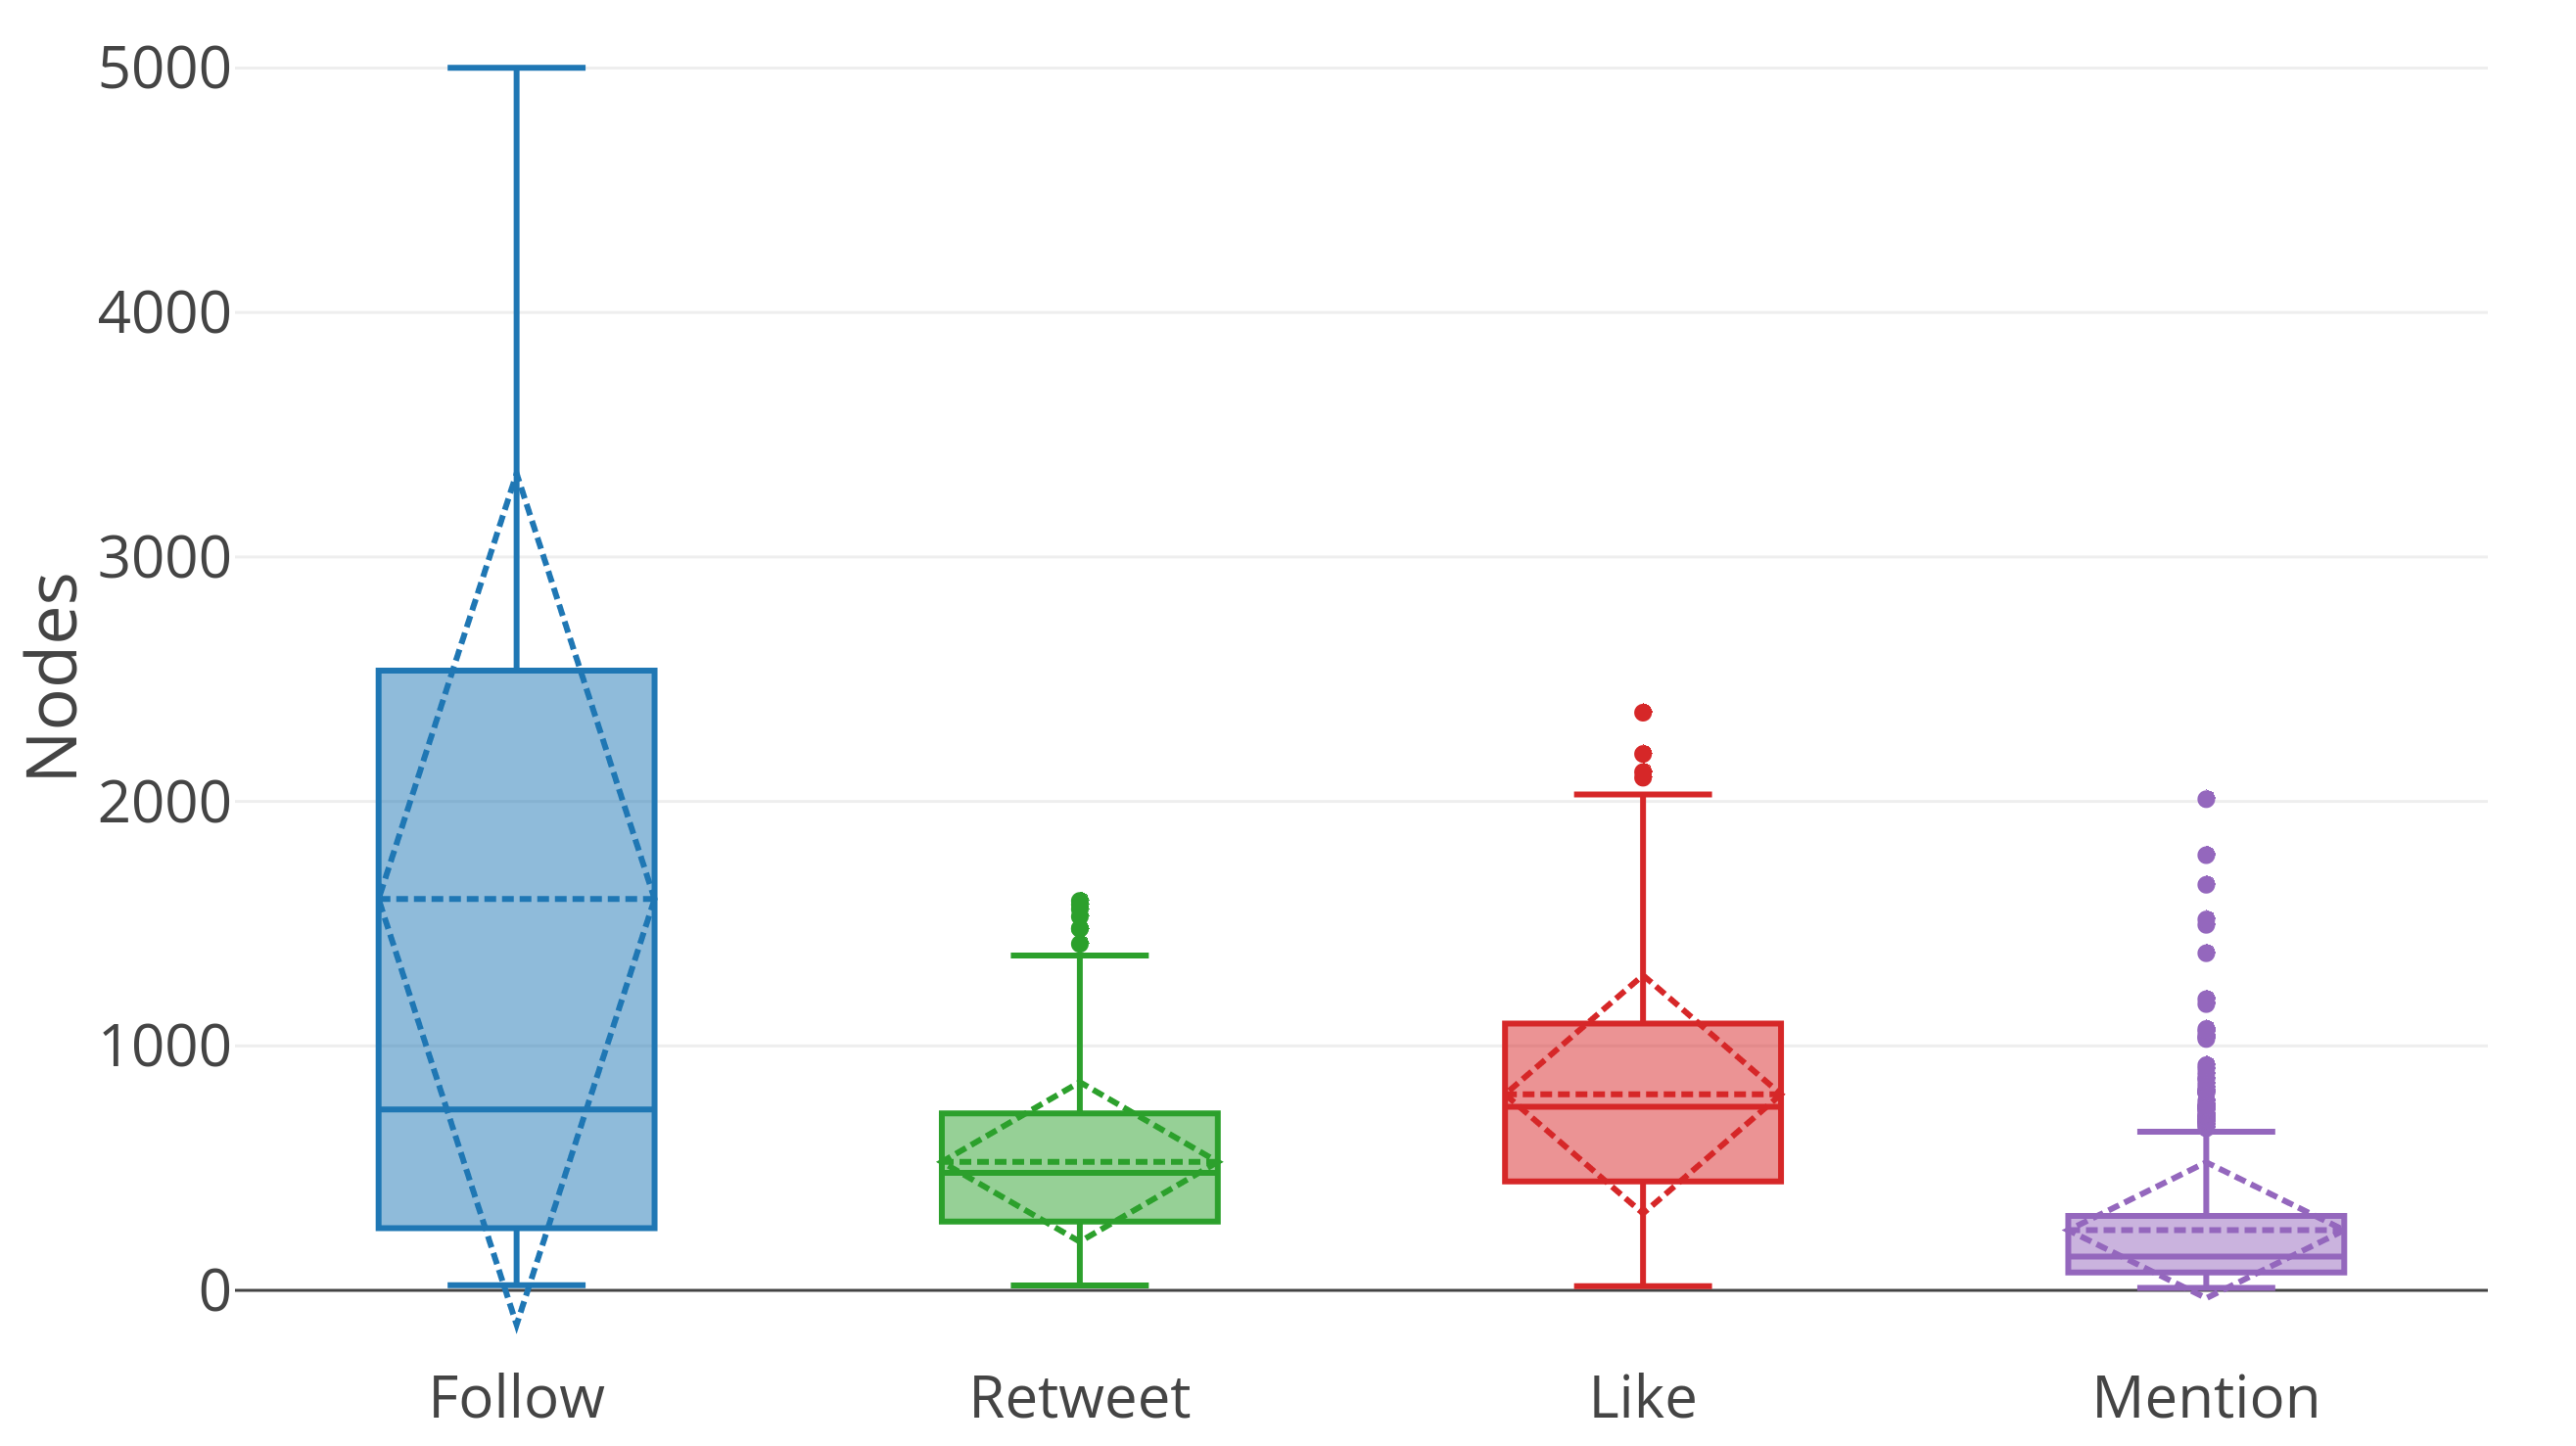
\includegraphics[width=1\textwidth]{fig/net_struct/number_of_nodes.png}
    \caption{Number of vertices in each layer.}
    \label{fig:net_struct_nodes}
\end{figure}


\begin{table}[h!tb]
    \renewcommand{\arraystretch}{1.3}
    \caption{Mean number of vertices, standard deviation, median, the minimum number and the maximum number of vertices found in each layer for the 500 ego networks.}
    \label{tab:numVertices}
    \centering
    \scriptsize
    \setlength\tabcolsep{6pt} % default value: 6pt
    \begin{tabular}{|c|c|c|c|c|c|}
    \hline
        {\bf Layer} &   {\bf Mean}  &   {\bf Stdv}  &   {\bf Median} & {\bf Min}  &   {\bf Max}  \\  \hline \hline
        Follow      &   1,600.77    &   1,742.74    &       740     &       21      &       5,001   \\  \hline
        Retweet    &   525.47      &   326.72      &       480.5   &       20      &       1,593   \\  \hline
        Like       &   801.84      &   487.79      &       750.5   &       17      &       2,363   \\  \hline
        Mention    &   246.08      &   278.31      &       138     &       10      &       2,009   \\  \hline \hline 
    \end{tabular}
\end{table}

\section{How the sizes of the ego networks vary among layers?}
\label{sec:net_structure}


We want to investigate the distribution of sizes of both number of vertices and number of edges in the four layers. Fig. \ref{fig:net_struct_nodes} present box plots of the distribution of the number of vertices in each layer of the 500 ego networks considered. Fig. \ref{fig:net_struct_edges} shows the distribution of the number of edges and Fig. \ref{fig:net_struct_density} shows the distribution of the density of edges in each layer. Tables \ref{tab:numVertices}, \ref{tab:numEdges} and \ref{tab:density} shows some additional information regarding the numbers of vertices, edges and the density of each layer. 

%%%%%%%%%%%%%%%%%%%%%%%%%%%%%%%%%%%%%%%%%%%%%% 
%%%%%%%%%%%%%%%%%%%%%%%%%%%%%%%%%%%%%%%%%%%%%% Edges

\begin{figure}[h!tb]
    \centering
    \begin{subfigure}
        \centering
        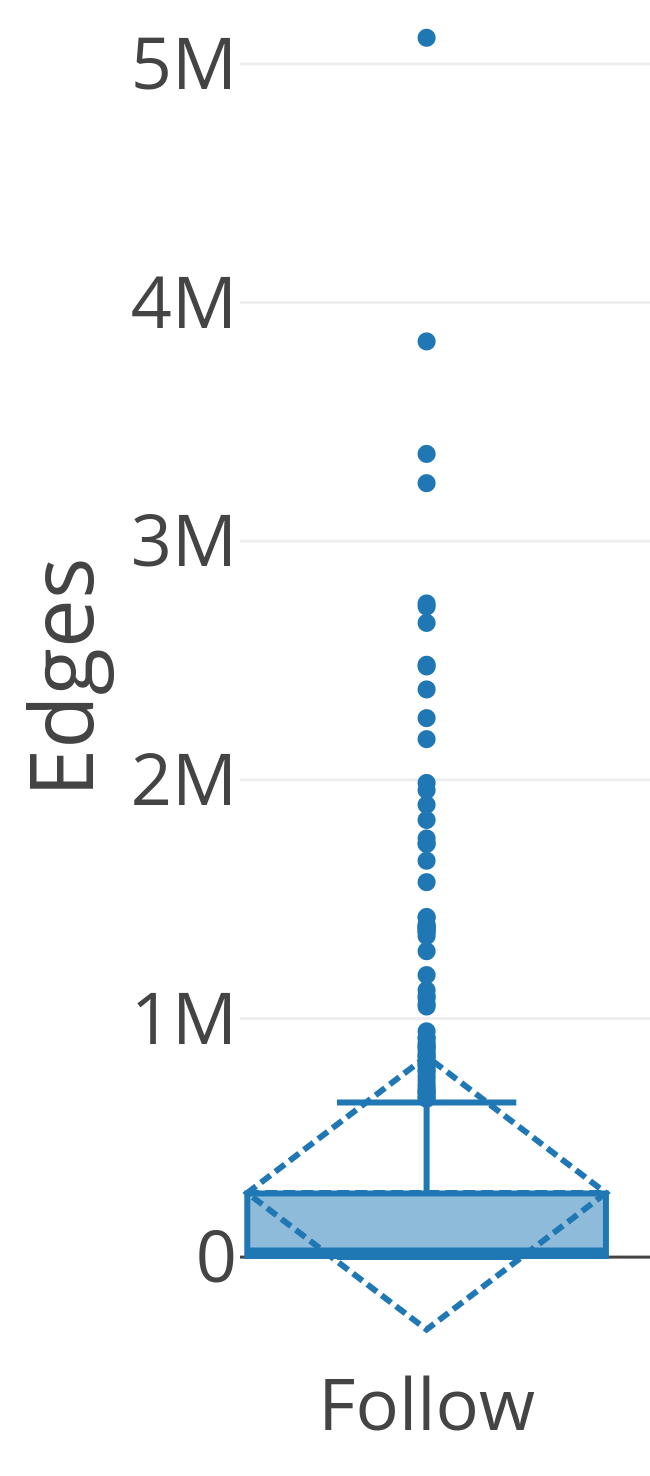
\includegraphics[width=0.23\textwidth]{fig/net_struct/number_edges_follow.png}
        %\caption{Follow}
    \end{subfigure}%
    ~ 
    \begin{subfigure}
        \centering
        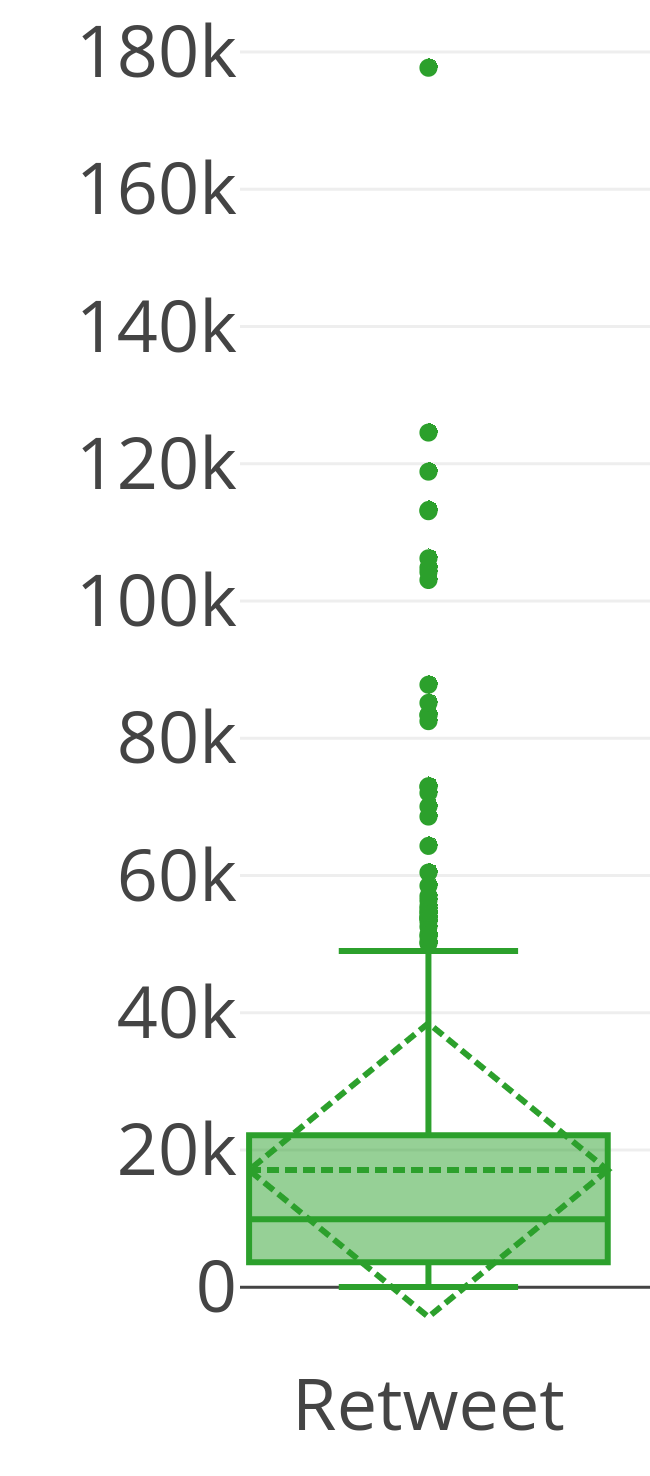
\includegraphics[width=0.23\textwidth]{fig/net_struct/number_edges_retweets.png}
        %\caption{Retweets}
    \end{subfigure}
    ~
    \begin{subfigure}
        \centering
        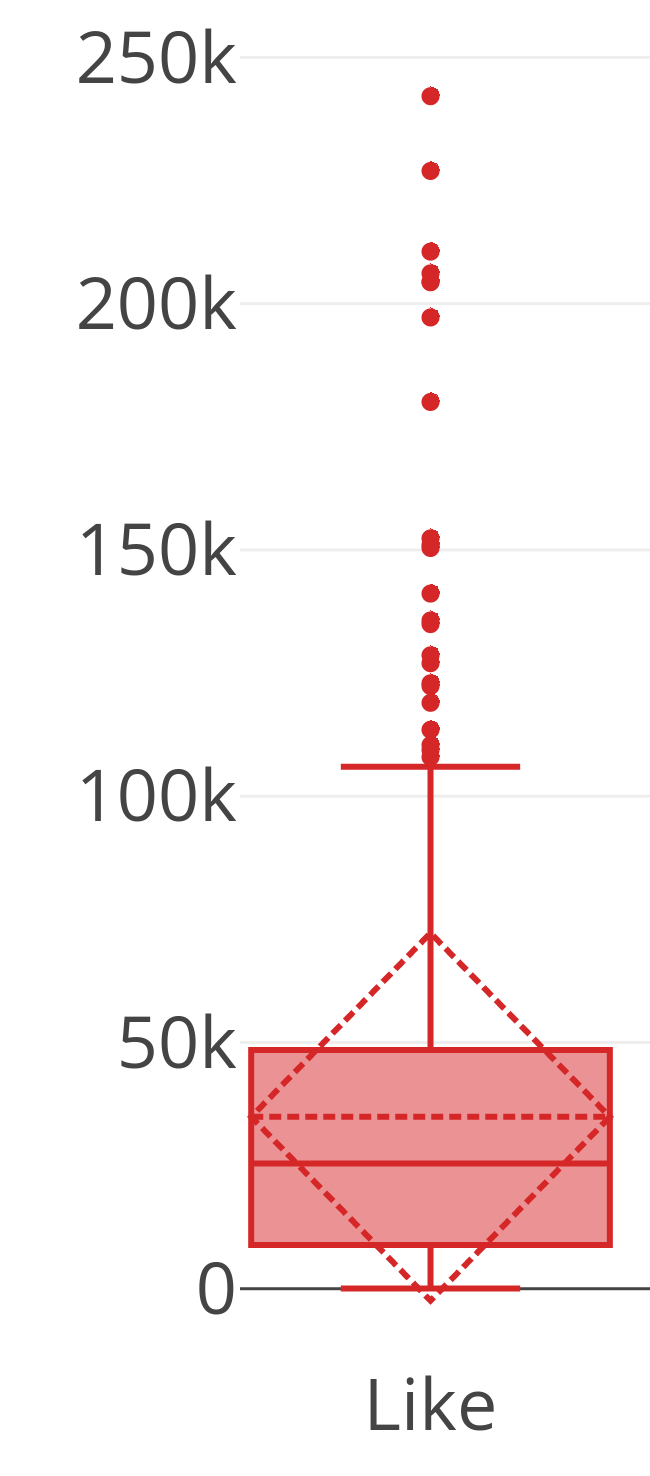
\includegraphics[width=0.23\textwidth]{fig/net_struct/number_edges_likes.png}
        %\caption{Likes}
    \end{subfigure}%
    ~ 
    \begin{subfigure}
        \centering
        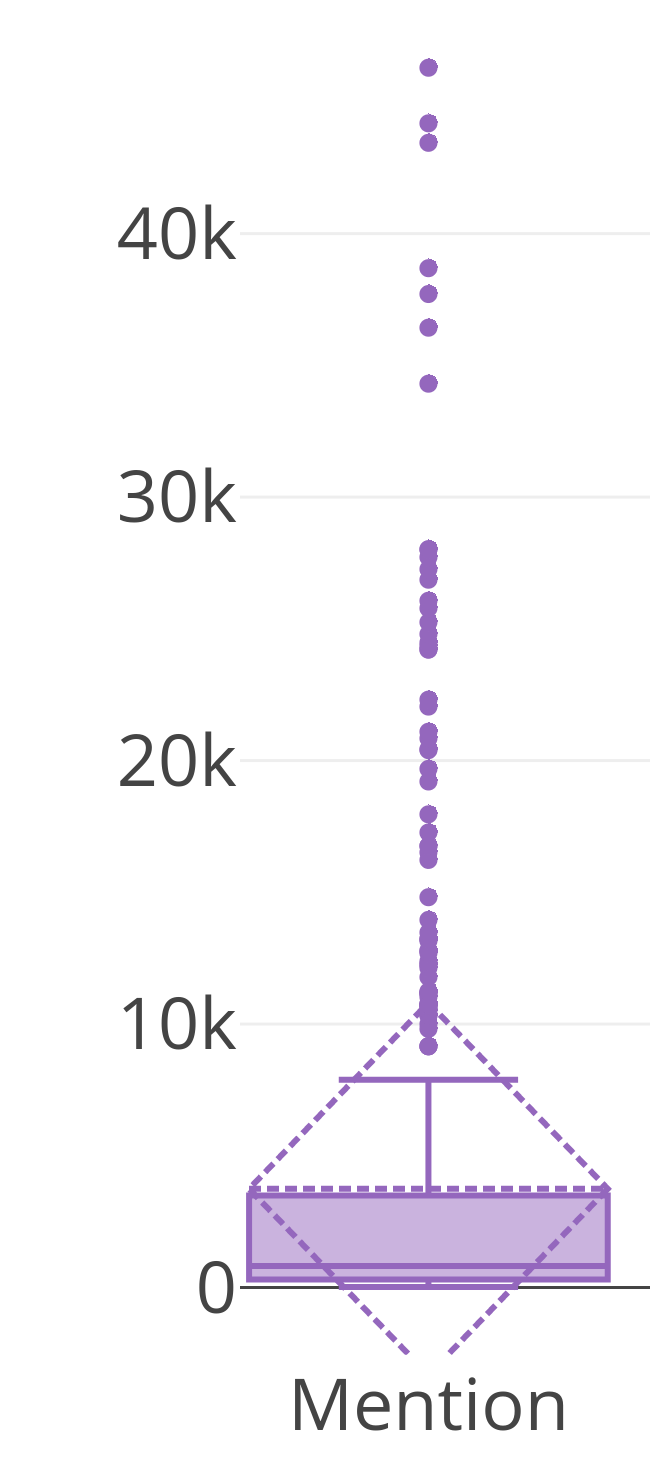
\includegraphics[width=0.23\textwidth]{fig/net_struct/number_edges_mentions.png}
        %\caption{Mentions}
    \end{subfigure}
    \caption{Number of edges in each layer.}
    \label{fig:net_struct_edges}
\end{figure}

\begin{table}[h!tb]
    \renewcommand{\arraystretch}{1.3}
    \caption{Mean number of edges, standard deviation, median, the minimum number and the maximum number of edges found in each layer for the 500 ego networks.}
    \label{tab:numEdges}
    \centering
    \scriptsize
    \setlength\tabcolsep{6pt} % default value: 6pt
        \begin{tabular}{|c|c|c|c|c|c|}
        \hline
        {\bf Layer} &   {\bf Mean}  &   {\bf Stdv}  &   {\bf Median}  &   {\bf Min}  &   {\bf Max}  \\ \hline \hline
        Follow      &   268,773.31  &   573,100.38  &   28,109.5    &       66      &   5,109,659   \\  \hline
        Retweet    &   17,073.12   &   21,423.85   &   9,917.5     &       31      &   177,702     \\  \hline
        Like       &   34,898.04   &   37,356.02   &   25,404.0    &       39      &   242,118     \\  \hline
        Mention    &   3,745.34    &   7,070.79    &   817         &       17      &   46,296      \\  \hline\hline 
    \end{tabular}
\end{table}

The number of vertices varies very much among egos for a same layer. The follow layer being the one with more intense variation. As shown in Fig. \ref{fig:net_struct_nodes}, half of the egos in our sample have up to 740 followees (alters), but the number of followees in the other half of the egos vary enormously, up to the limit of 5.000 followees. In the other three layers there is also a great variation, as can be seen by the standard deviation values in Fig. \ref{tab:numVertices}, but it is not so high as in the case of the follow layer. 

It is also interesting to notice that the number of alters in the mention layers is usually less than in all the other layers for all egos. This seems to reflect the nature of this interaction. A mention is a direct communication between two users via a tweet. It implies in a certain acquaintance between the sender and the receiver of the tweet. This naturally implies in a restriction on the number of alters. The same does not necessary occurs with like and retweet layers, because a user may retweet or like a tweet independently if she knows or not its author.


%%%%%%%%%%%%%%%%%%%%%%%%%%%%%%%%%%%%%%%%%%%%%% 
%%%%%%%%%%%%%%%%%%%%%%%%%%%%%%%%%%%%%%%%%%%%%% Density

\begin{figure}[h!tb]
    \centering
    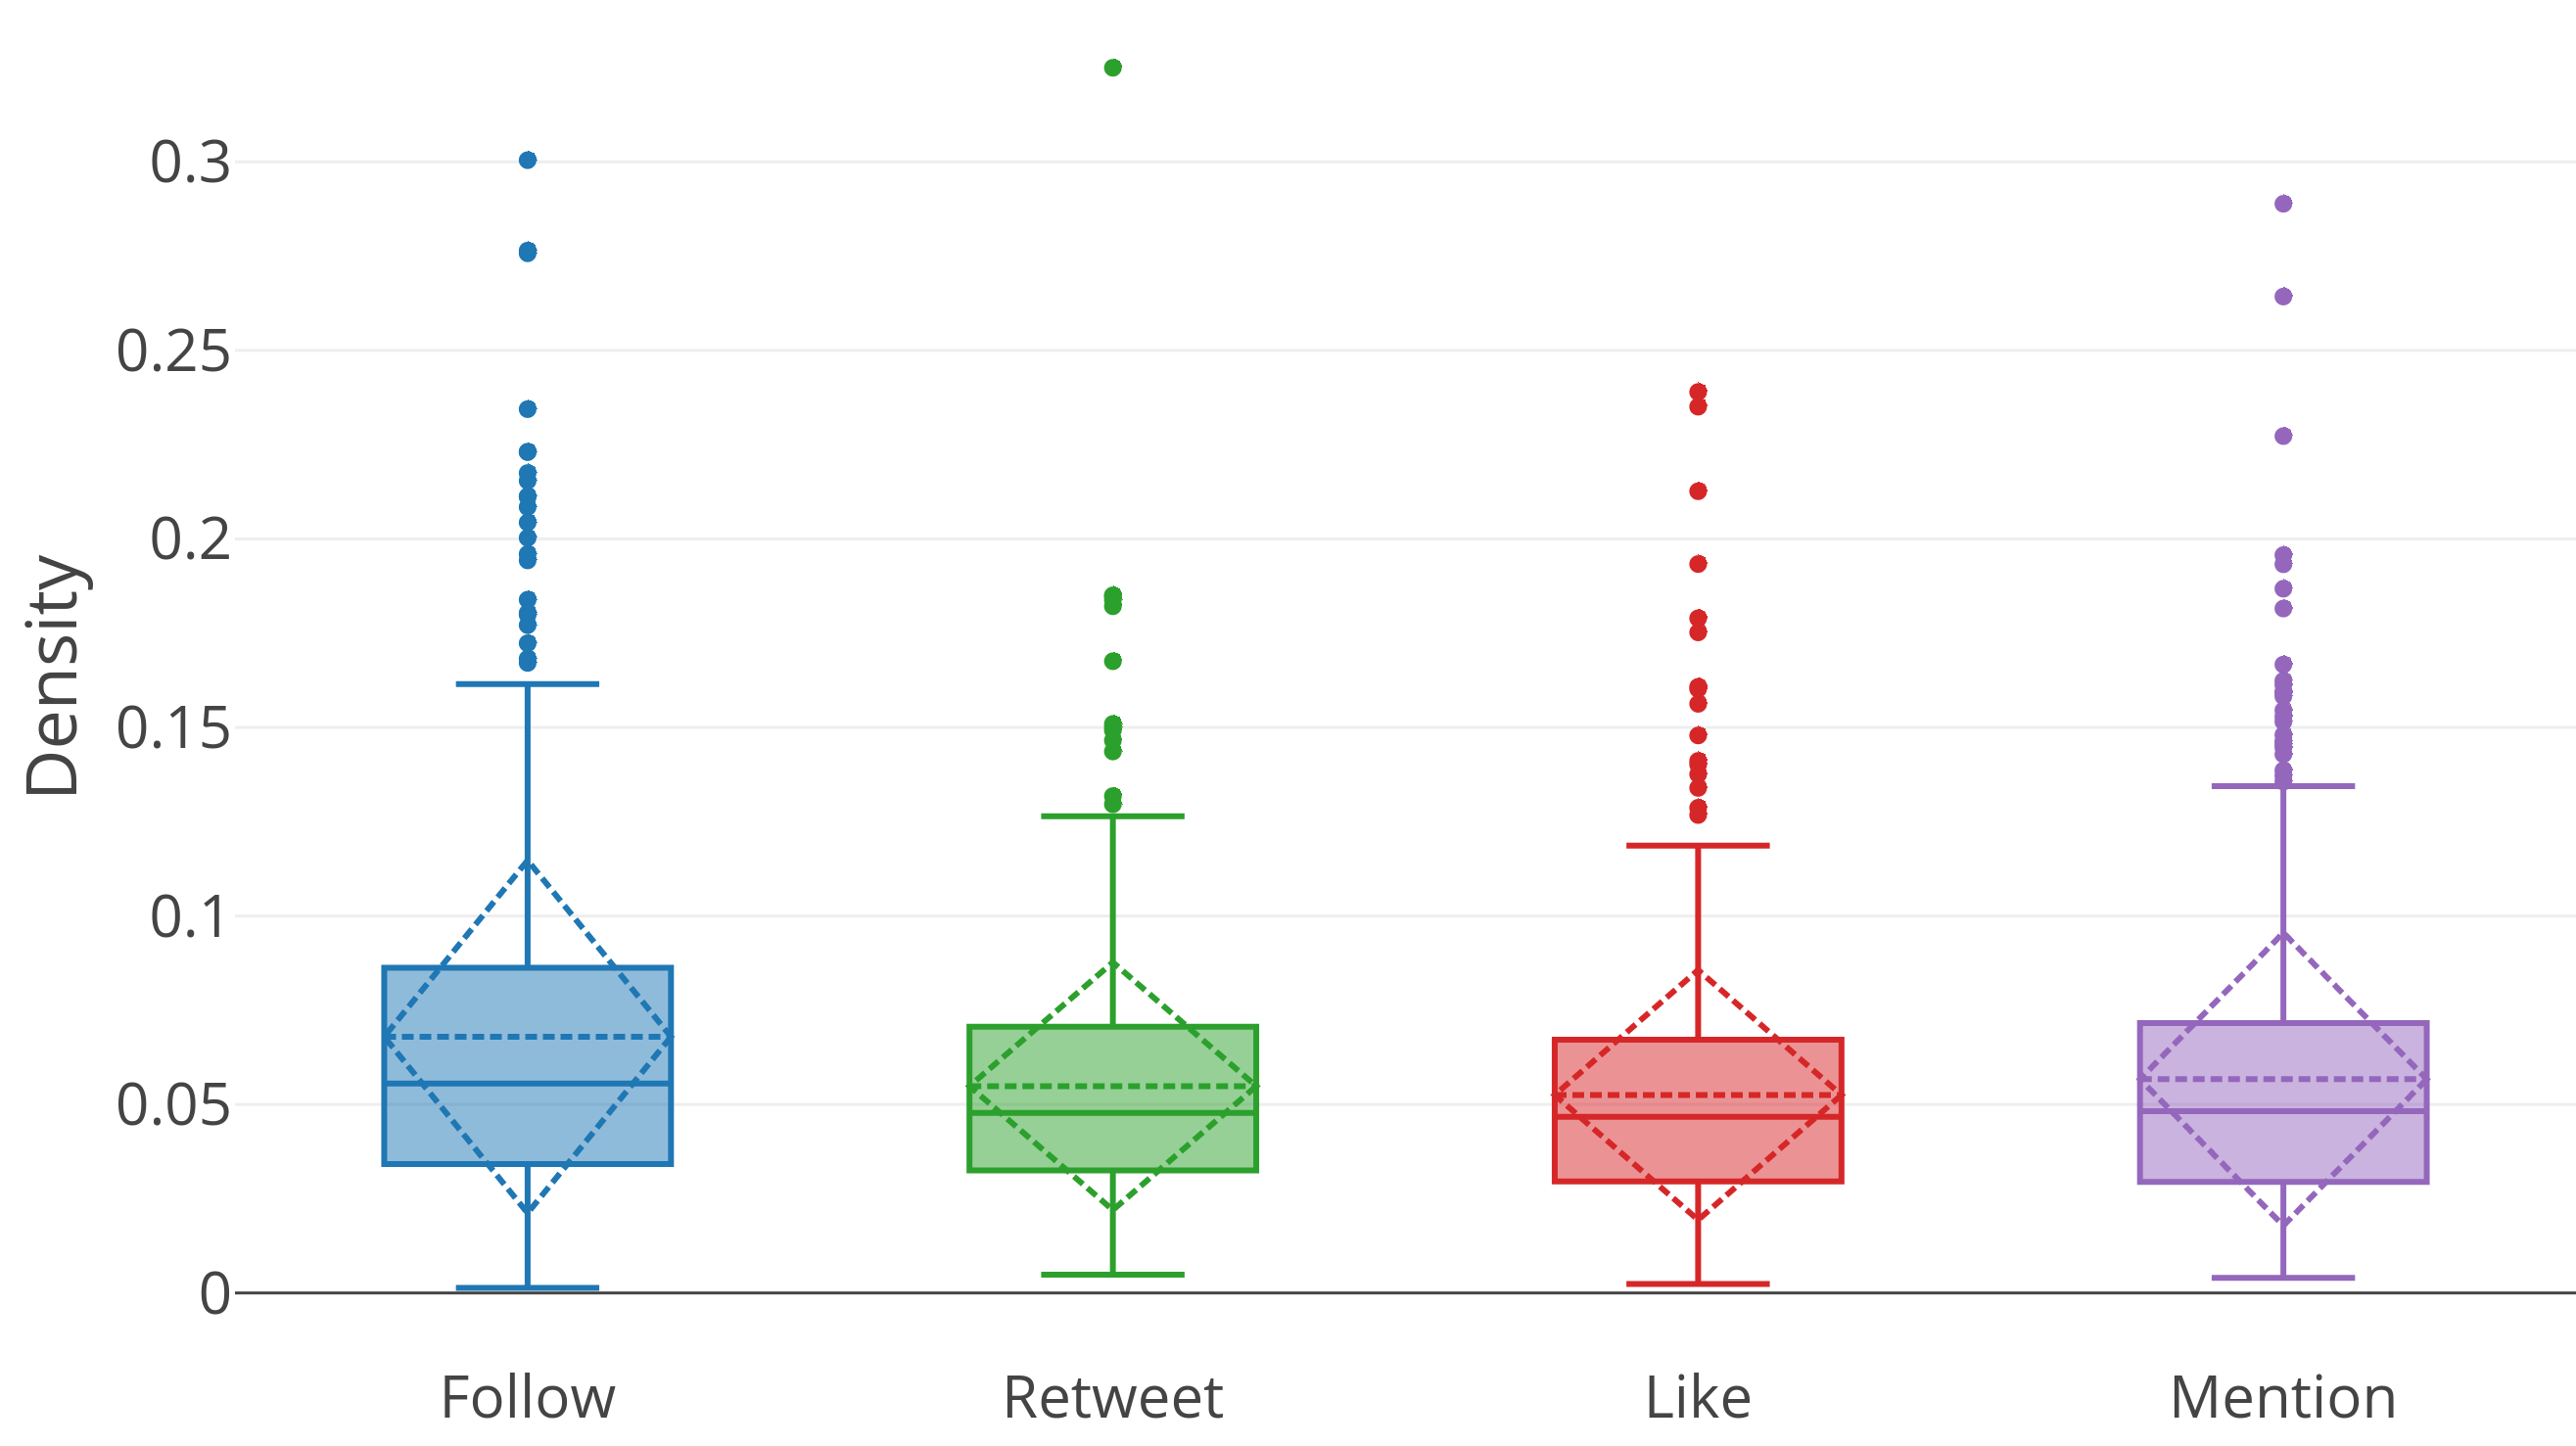
\includegraphics[width=1\textwidth]{fig/net_struct/density.png}
    \caption{Density of edges in each layer.}
    \label{fig:net_struct_density}
\end{figure}

\begin{table}[h!tb]
    \renewcommand{\arraystretch}{1.3}
    \caption{Mean, standard deviation, median, the minimum and the maximum value of density found in each layer for the 500 ego networks.}
    \label{tab:density}
    \centering
    \scriptsize
    \setlength\tabcolsep{6pt} % default value: 6pt
    \begin{tabular}{|c|c|c|c|c|c|}
        \hline
        {\bf Layer} &   {\bf Mean}  & {\bf Stdv}  & {\bf Median} & {\bf Min} & {\bf Max}  \\  \hline \hline
        Follow     &    0.0680    &   0.0468  &     0.0556      &  0.0013   &  0.3005\\  \hline
        Retweet    &    0.0548    &   0.0329  &     0.0478      &  0.0048   &  0.3250\\  \hline
        Like       &    0.0525    &   0.0331  &     0.0467      &  0.0024   &  0.2390\\  \hline
        Mention    &    0.0567    &   0.0388  &     0.0482      &  0.0040   &  0.2889\\  \hline \hline 
    \end{tabular}
\end{table}

Fig. \ref{fig:net_struct_edges}  shows also  a great variation on the number of edges in all layers. However, when observing the density distribution of all this layers in Fig. \ref{fig:net_struct_density} we can see that independent of the so large differences on the number of edges and vertices among egos in all layers, the distributions of edges in the graphs are equally very sparse. We have very few edges in all layers of all ego networks compared to the possible number of edges that could exist (i.e $|\{e\}\cup A_e^i|(|\{e\}\cup A_e^i|-1)$ for a layer $i$). In fact, 75\% of the egos have edge density inferior to 0.1 in all layers. This implies that most alters interact only with a small fraction of the same layer members, including the ego and the other alters. In other words, the intersections of the alter set of an ego  $e$ and the alter sets of her alters are very small in all layers.

\begin{figure}[h!tb]
    \centering
    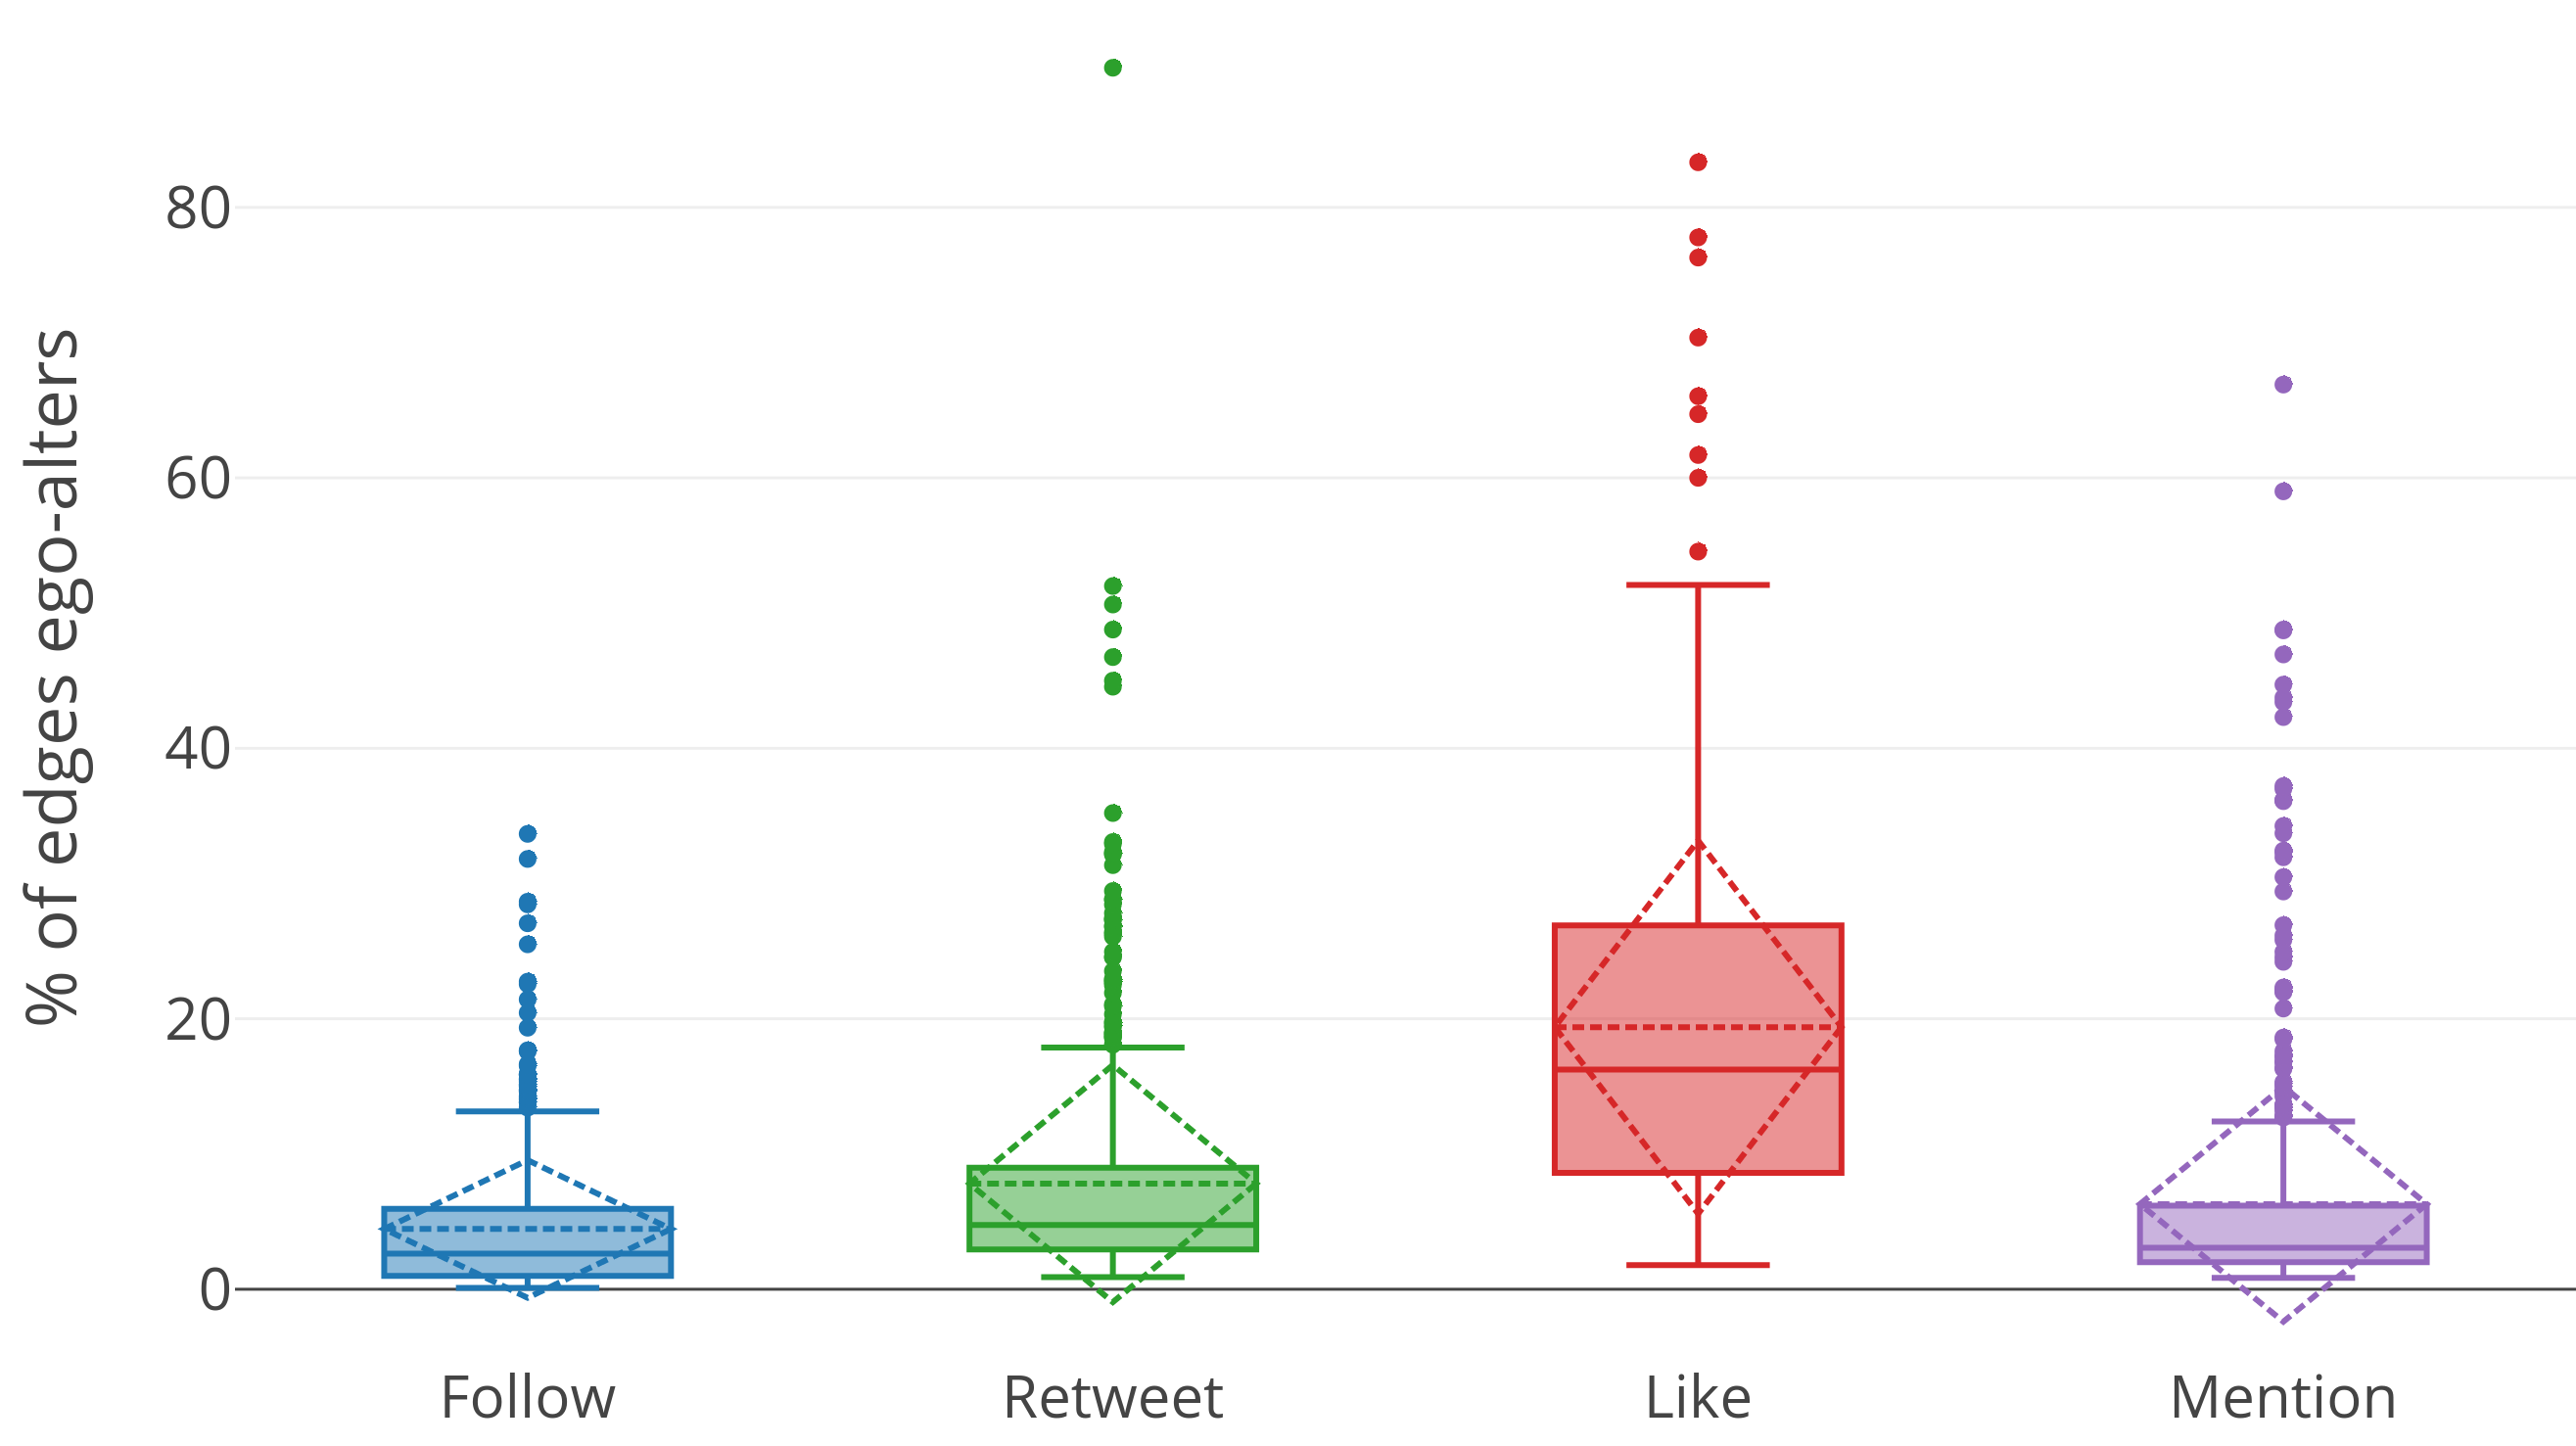
\includegraphics[width=1\textwidth]{fig/net_struct/edges_ego_alters.png}
    \caption{Percentage of edges ego-alters.}
    \label{fig:net_struct_edges_ego_alters}
\end{figure}

As the edge density is low, the number of edges that start from the ego and arrive at the alter is also low, according to the results presented in Fig. \ref{fig:net_struct_edges_ego_alters}. The users with whom the ego interacts also interact with each other or interact back with the ego using the same type of interaction, with almost all ego networks having a number of ego-alters edges less than 20\%. Except is due to the like layer, where the number of ego-alters edges is on average close to 20\%. This result shows that all ego networks are sparse, but among the existing edges there are a significant number of edges that start from the alters and therefore the ego networks are not mostly formed by ego-alters edges.

We also investigated if there is a correlation of the number of alters in different layers for an ego. If the correlation value of the number of egos between two layer of an ego is high, this could be a characteristic of the ego profile, i.e., introspective egos would tend to have a small set of alters in all layers and more communicative egos would have a great number of alters in all layers. However, as Fig. \ref{fig:net_struct_nodes_correlation} shows, we have strong values of the Spearman correlation between the pair of layers (like, retweet) and  (follow, mention) layers; and weak values between (follow, like). There is practically no correlation between the pairs (follow, retweet) and (like, mention); and the (retweet, mention) layers has a moderate negative correlation. Thus, we can conclude that usually a user does not follow a same pattern when interacting with all different types of interaction in Twitter, regarding the number of people she interact with different types of interaction.

\begin{figure}[h!tb]
    \centering
    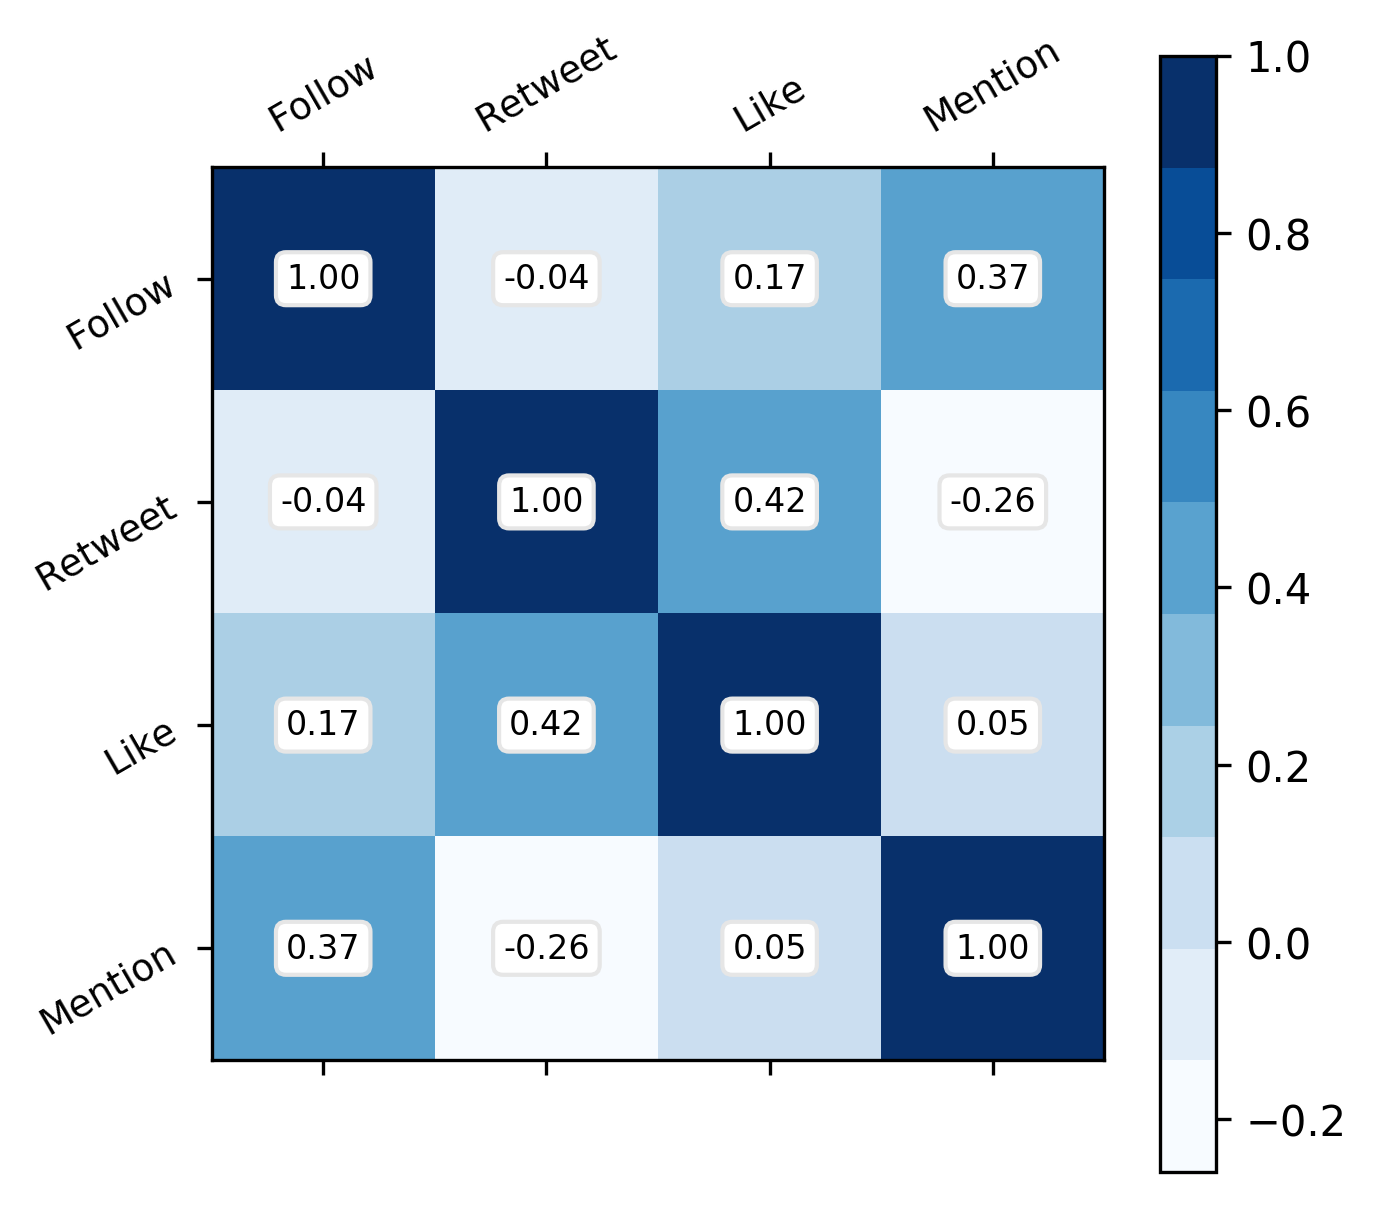
\includegraphics[width=0.8\textwidth]{fig/net_struct/nodes_correlation_spearman.png}
    \caption{Vertices Spearman's Correlation inter-layers.}
    \label{fig:net_struct_nodes_correlation}
\end{figure}

The standard deviation presented in the Tab. \ref{tab:numVertices} reveals that the variation in the size of the retweet and like layers (alters set) is much smaller when compared to the follow and mention networks, which seems to be a pattern in the behavior of users regarding the ability to interact with different alters - there seems to be a tendency for stabilization/saturation in the size of the retweet and like layers. While in the follow and mention layers the size of the set of alters varies greatly from one ego to another, in the retweet and like layers the size of the set seems to converge to a mean value. The results observed in Fig. \ref{fig:net_struct_nodes_correlation} also reinforce the idea that there is a tendency of stabilization in the size of the retweet and like layers because there is a strong correlation between these two layers, and by the convergence in the number of alters.

We also note that there is a moderate correlation between the size of the layers (follow, mention), indicating that the ability to mention distinct alters correlates with the number of users that the ego follows. The higher the number of alter in the follow layer, the greater the number of alters in the mention layer, unlike the results of the correlation between (follow,retweet) and (follow,like) layers, showing that the number of alters in the follow layer has practically no correlation with the number of alters of the retweet layer and a weak correlation with the number of alters of the like layer. 



%%%%%%%%%%%%%%%%%%%%%%%%%%%%%%%%%%%%%%%%%%%%%% 
%%%%%%%%%%%%%%%%%%%%%%%%%%%%%%%%%%%%%%%%%%%%%% Questions
%%%%%%%%%%%%%%%%%%%%%%%%%%%%%%%%%%%%%%%%%%%%%% 
%%%%%%%%%%%%%%%%%%%%%%%%%%%%%%%%%%%%%%%%%%%%%% 
\subsection*{How reciprocal are the relations inside each layer?}
\label{subsec:reciprocity_result}
\begin{figure}[h!tb]
    \centering
    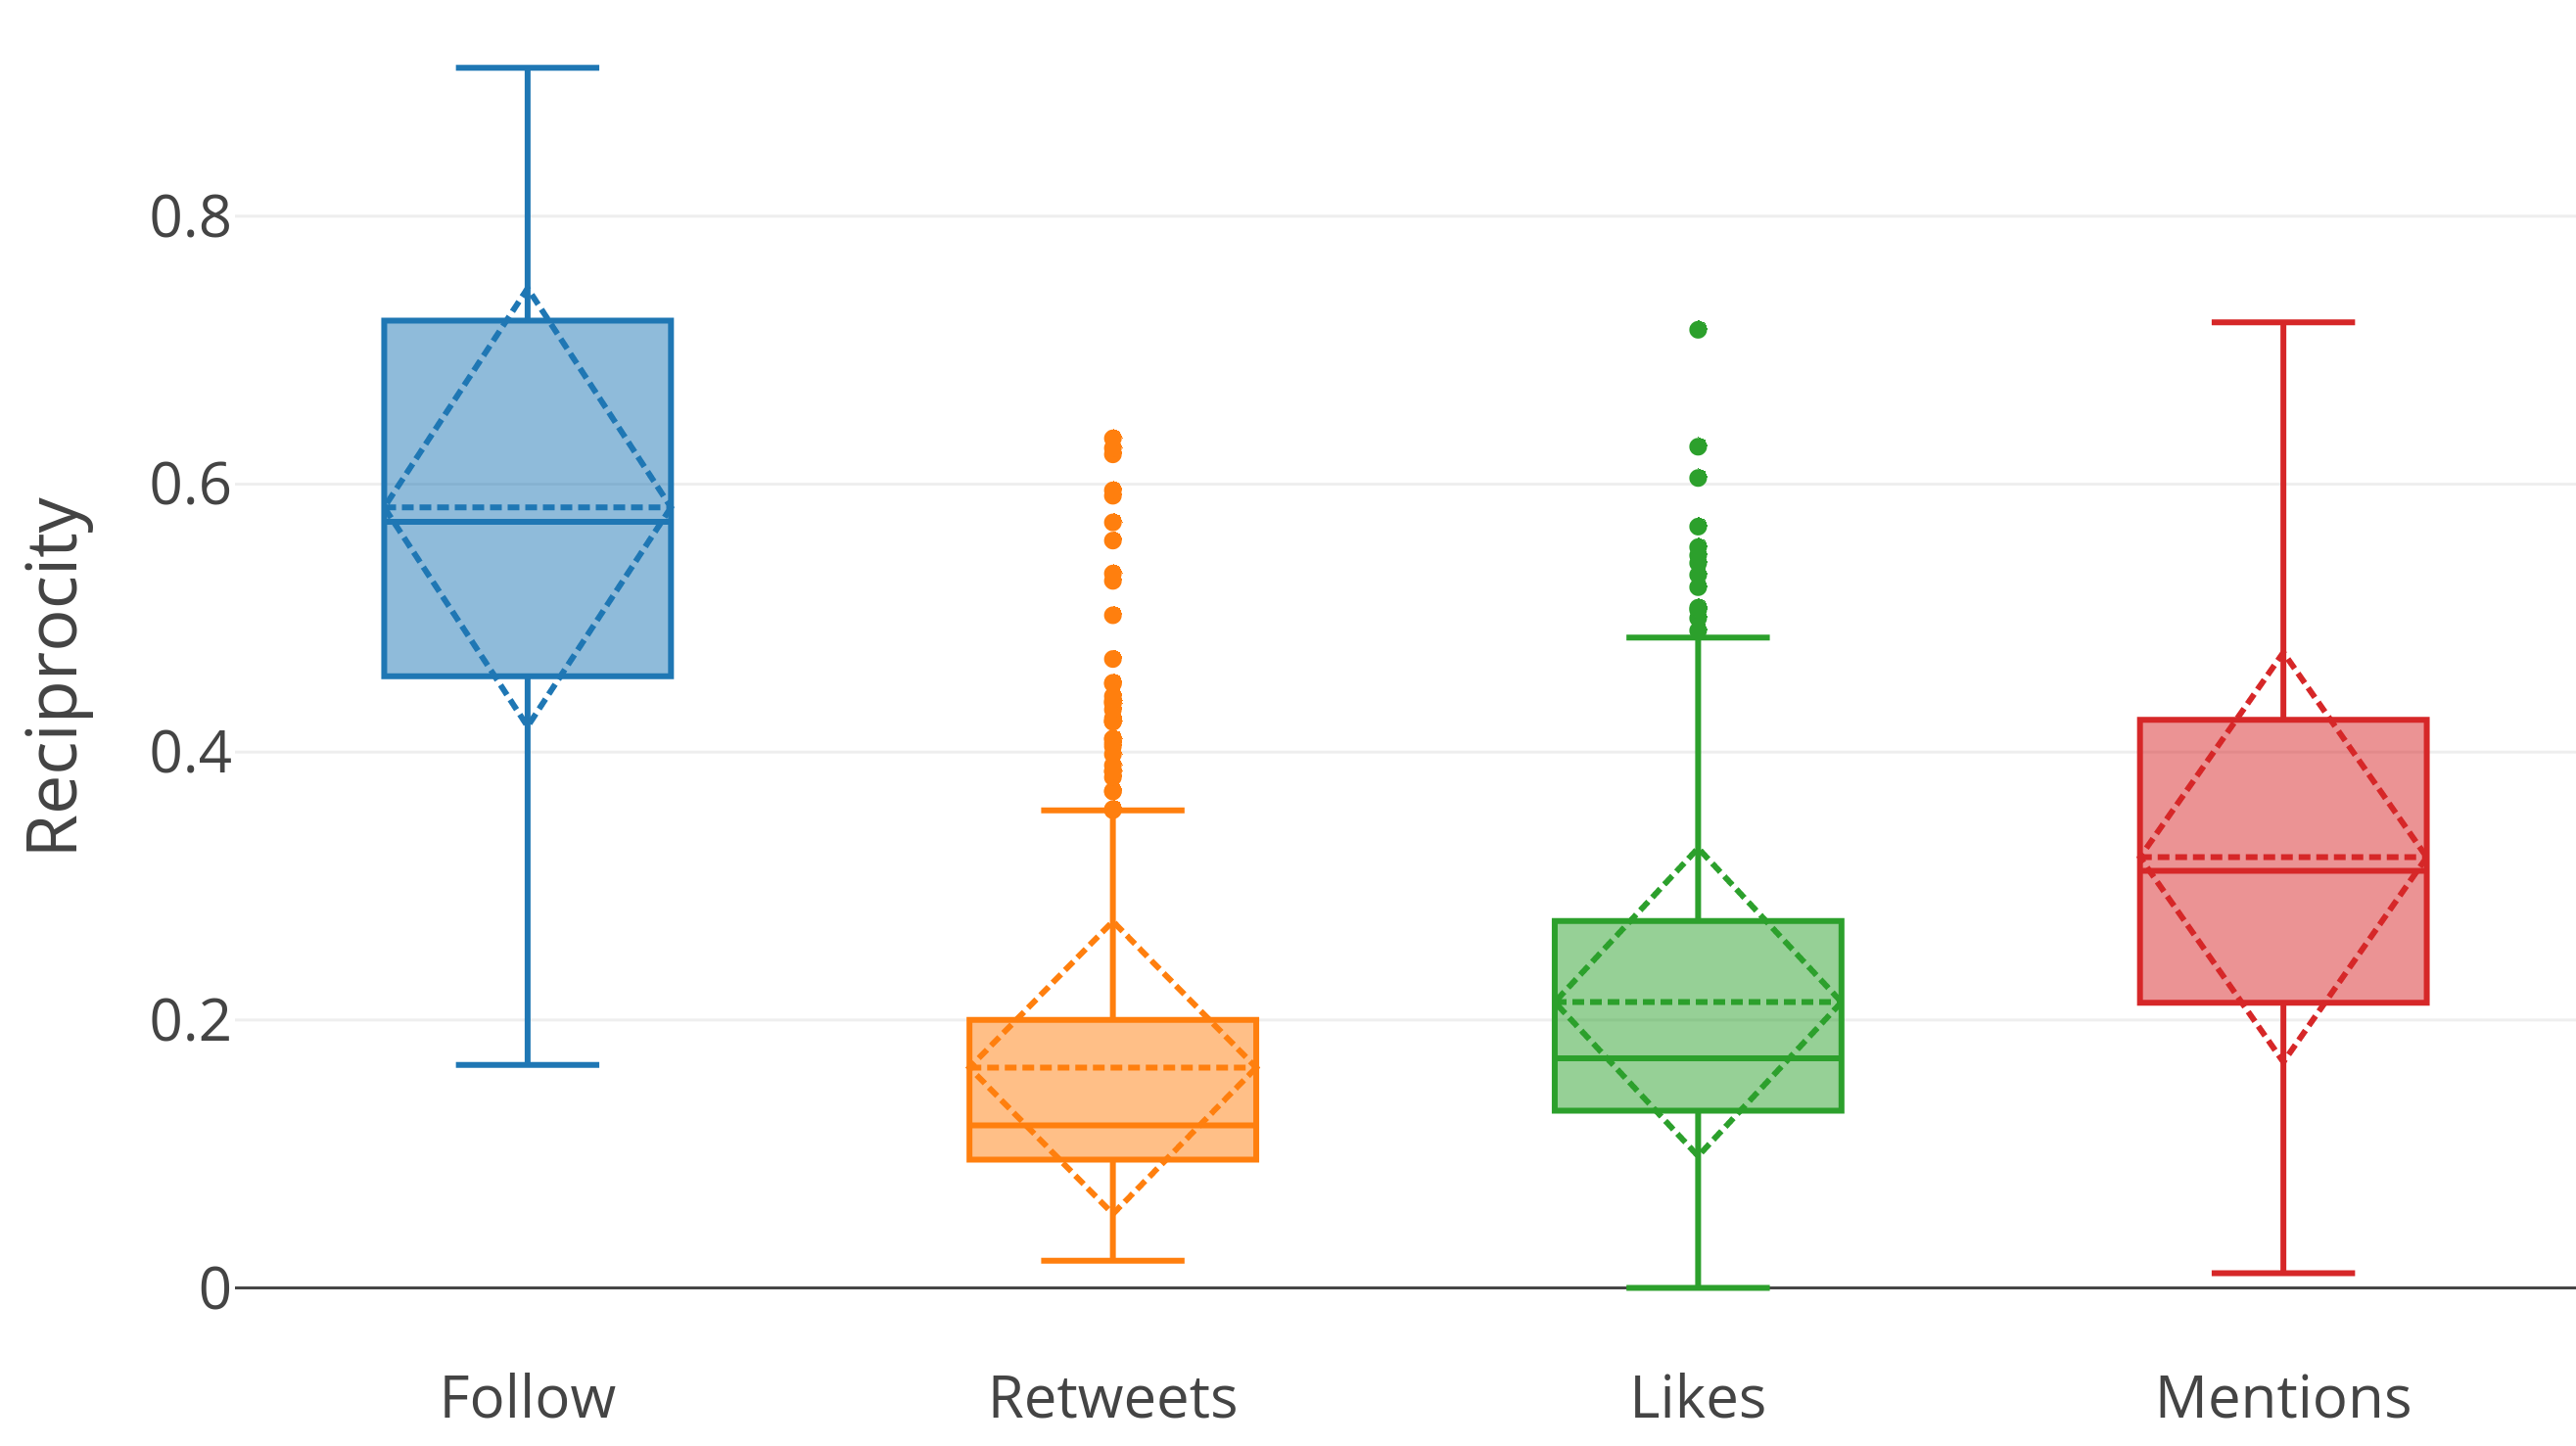
\includegraphics[width=1\textwidth]{fig/net_struct/reciprocity.png}
    \caption{Reciprocity.}
    \label{fig:net_struct_reciprocity}
\end{figure}

Reciprocity evaluates whether interactions between users in a particular layer occur reciprocally, or are predominantly unidirectional interactions, and was computed using Eq. \ref{eq:reciprocity}. The results of reciprocity in multilayer ego networks reveal important differences among layers, as can be seen in Fig \ref{fig:net_struct_reciprocity}. The follow layer has the greatest values. However, Twitter user interface allows a user to see all her followers and to choose to follow back any of them. This may be a great incentive for reciprocity in the follow layer. 

On the other hand, it is interesting to see in the case of dynamic operations as like, follow and mention, how they influence reciprocity. While the first two operations work as endorsements of having read a good tweet and indirectly as endorsement of the writer as a good author, mention tends to imply at least a short term engagement between two users. That is because a mention works as a direct message from one person to the other and a received message tends to induce a response message. Results in the Fig \ref{fig:net_struct_reciprocity} seem to reflect these observations. We can see that reciprocity values for retweet an like layers are similar and small while numbers for the mention layer are comparatively bigger.


\section{How similar are the layers of Twitter multilayer ego networks?}
\label{sec:QuestionSimilarLayers}

In this section we investigate how similar two graphs corresponding to two different layers  of an ego network are. To answer this question, we need to know how similar the vertices set and the edges sets of two distinct layers are. The measure of these similarities reveal two information: a) Is the set of people an ego interacts to with interaction type $x$ similar to the set of people she interacts to with interaction type $y$? b) Interactions between two individuals in one layer repeat in other layers?

%%%%%%%%%%%%%%%%%%%%%%%%%%%%%%%%%%%%%%%%%%%%%% 
%%%%%%%%%%%%%%%%%%%%%%%%%%%%%%%%%%%%%%%%%%%%%% Vertex Overlap
\subsection*{Vertex Overlap}
\label{subsec:vertex_overlap}

\begin{figure}[h!tb]
    \centering
    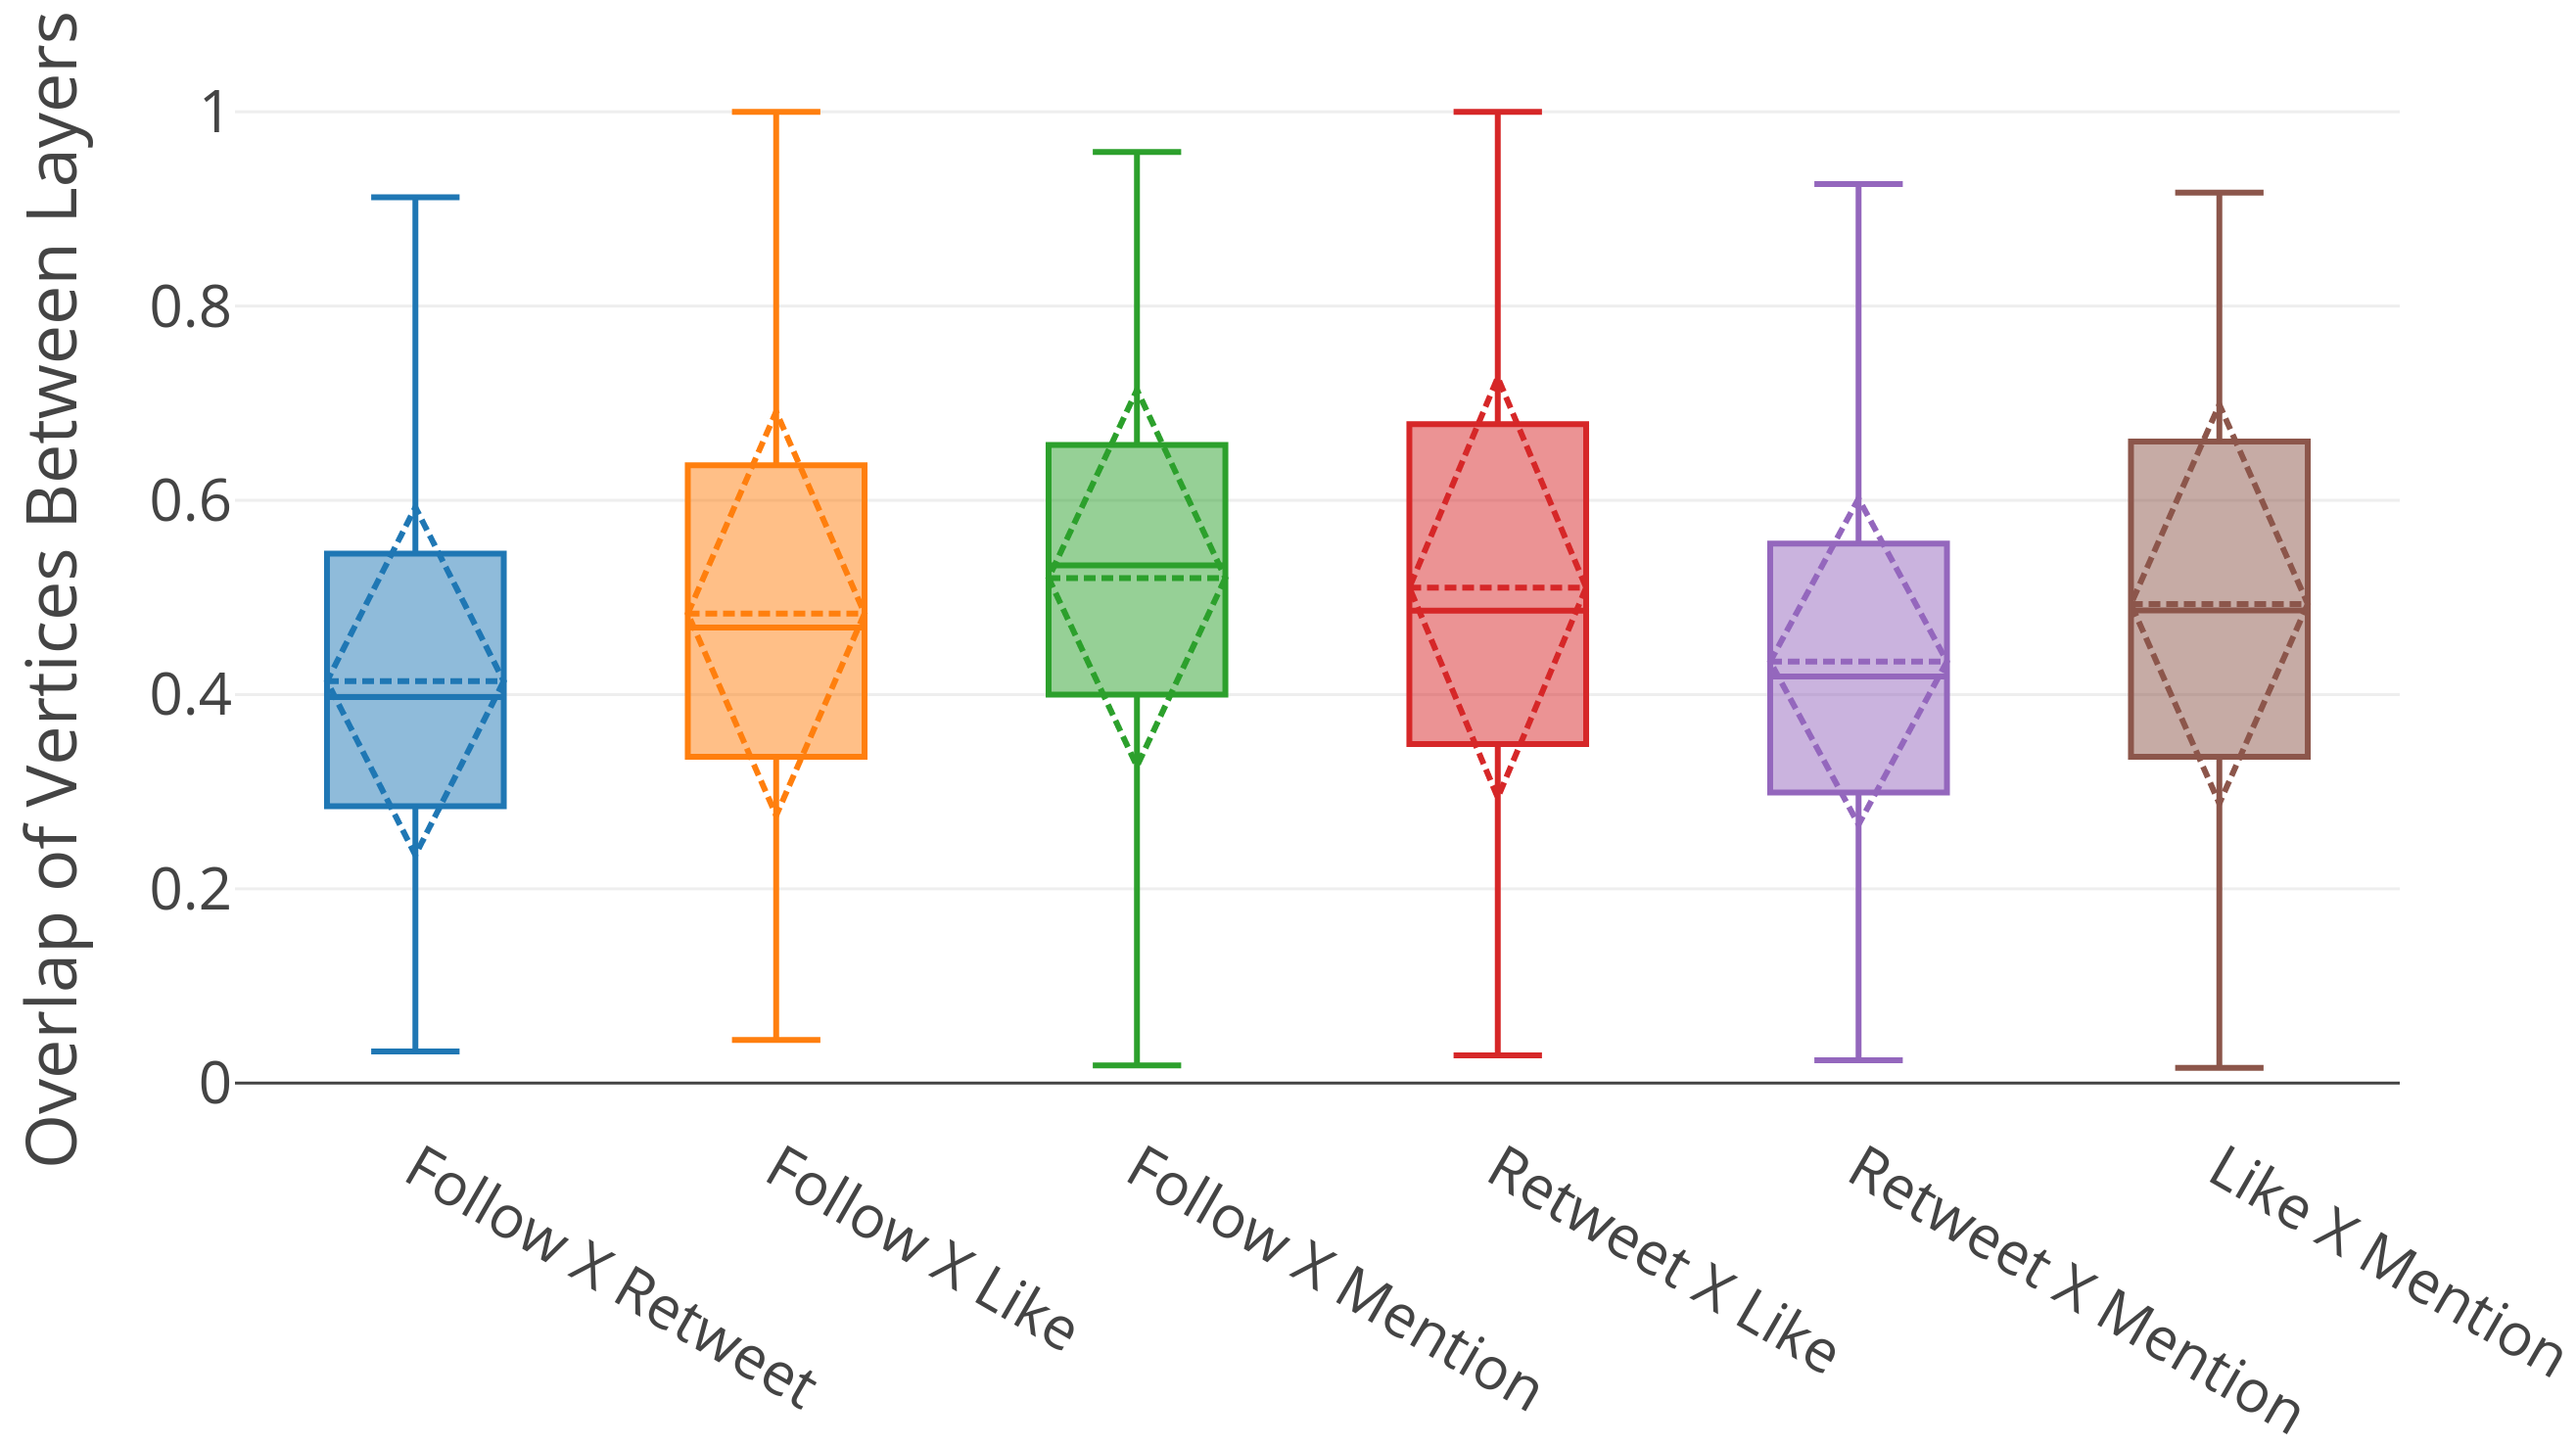
\includegraphics[width=1\textwidth]{fig/net_struct/overlap/overlap_vertices_boxplot.png}
    \caption{Vertex overlap between layers.}
    \label{fig:net_struct_overlap_vertices_boxplot}
\end{figure}

Fig. \ref{fig:net_struct_overlap_vertices_boxplot} shows that there is a great variability of vertex overlap for a given pair of layers, with some egos with almost zero vertex overlap between layers and some with almost 100\% of vertex overlap. However, most egos (those in interquartile)  have some alter overlap between layers. For instance, 50\% of egos have overlap values between 0.2 to almost 0.6 for the pairs (follow, retweet) and (retweet, mention) and 25\% of the egos have vertex overlap superior do 0.6 in these layers. In other pairs, vertex overlap are slightly greater. This means that for about 75\% of egos at least 20\% of their alters in a layer $x$ also occur in layer $y$, for $|A^x| \leq |A^y|$ (according to definition of overlap adopted -- see Eq. \ref{eq:overlap}. It can be seen that the pair (follow, mention) tends to have more vertex overlap values than the other pairs, meaning that people that an ego mentions tend to be her followees. 

Thus, most egos present some overlap among their alters sets belonging to different layers, but the set of vertices are still distinct between pairs of layers, with at least 30\% of the alters in the smaller layer not occurring in the bigger one, in most cases (see the third quartile not reaching 70\% of overlap in any layer). 


%%%%%%%%%%%%%%%%%%%%%%%%%%%%%%%%%%%%%%%%%%%%%% 
%%%%%%%%%%%%%%%%%%%%%%%%%%%%%%%%%%%%%%%%%%%%%% Edge Overlap
\subsection*{Edge Overlap}
\label{subsec:edge_overlap}

\begin{figure}[h!tb]
    \centering
    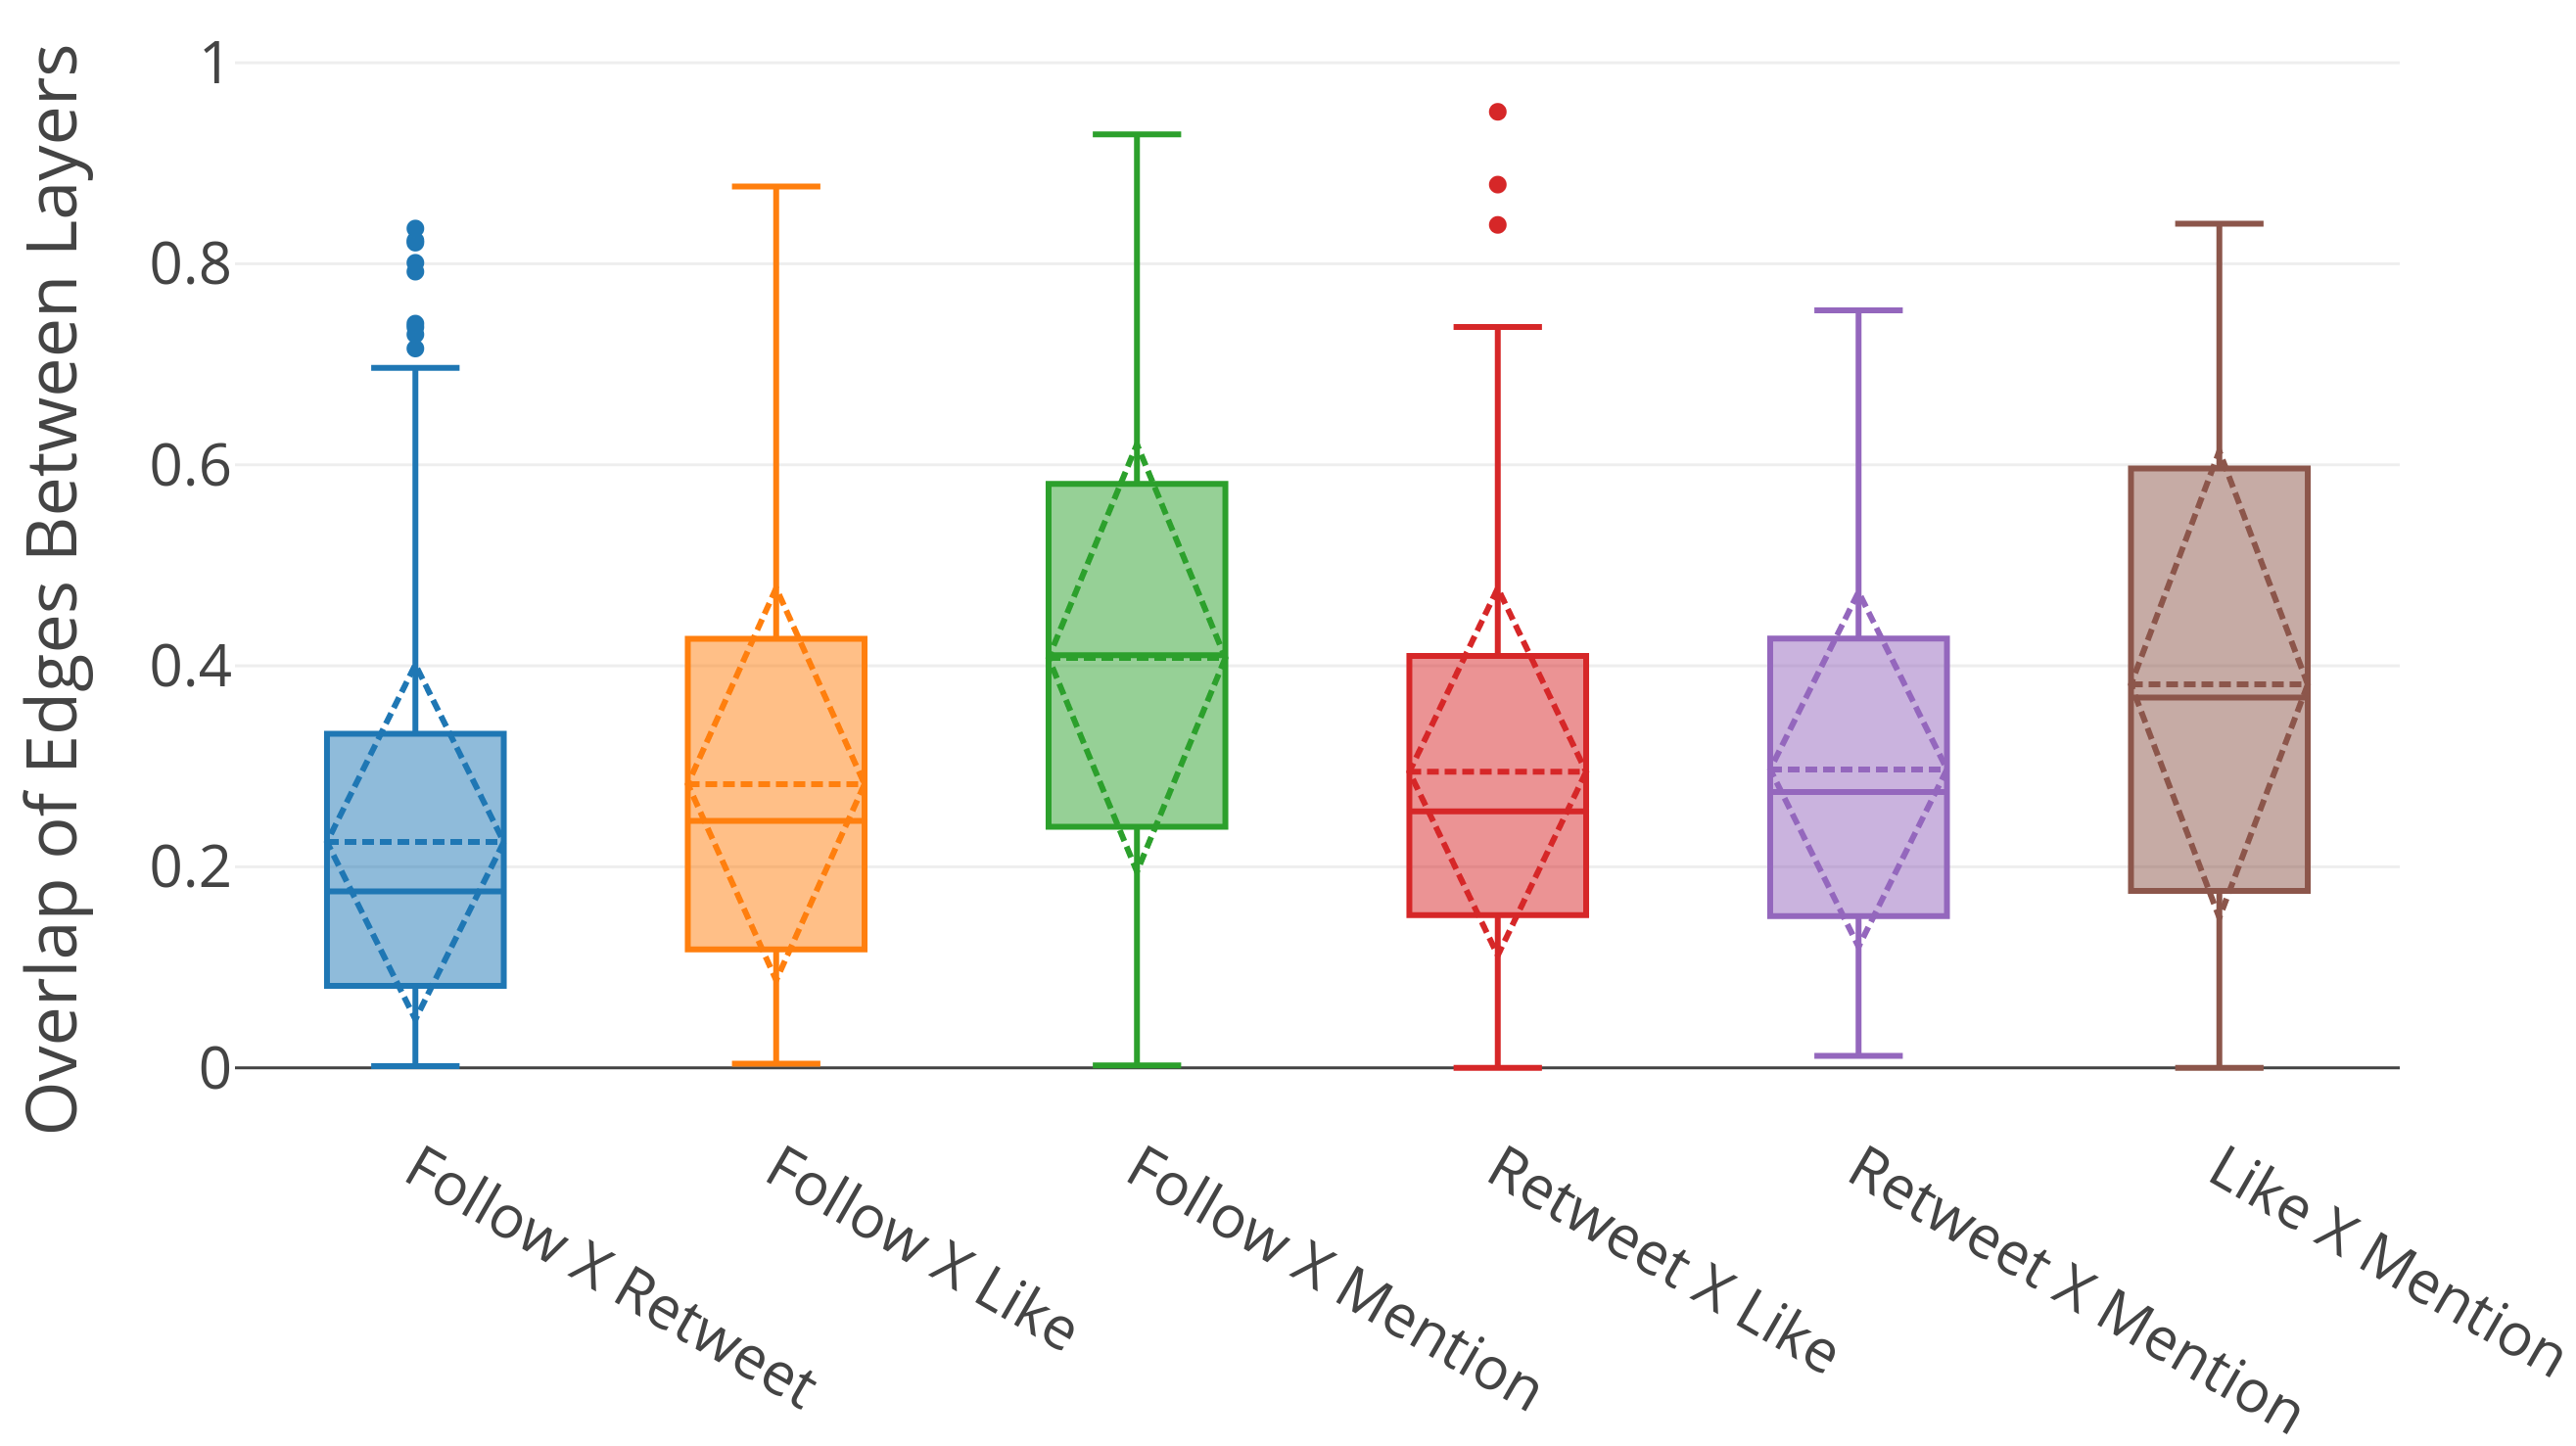
\includegraphics[width=1\textwidth]{fig/net_struct/overlap/overlap_edges_boxplot.png}
    \caption{Overlap of edges between layers.}
    \label{fig:net_struct_overlap_edges_boxplot}
\end{figure}

Edge overlap values are even smaller than vertex overlap values as shows Fig. \ref{fig:net_struct_overlap_edges_boxplot}, but, considering the small values of edge density in all layers, there still are considerable overlap, especially between the following pairs: (follow, mention) and (like, mention) with 50\% of the egos with overlay values varying between 20\% to 60\% in these layers. For the other pairs of layers, edge overlap is predominantly small, with about 75\% of the egos achieving at most 40\% of overlap values.


%%%%%%%%%%%%%%%%%%%%%%%%%%%%%%%%%%%%%%%%%%%%%% 
%%%%%%%%%%%%%%%%%%%%%%%%%%%%%%%%%%%%%%%%%%%%%% RBO
\subsection*{Rank-Biased Overlap}
\label{subsec:rbo}
Another relevant aspect of layer similarity is how many of the most important vertices in one layer are also the most important vertices in the other layer. In social networks, one common measure of importance is vertex indegree, defined in Section \ref{subsec:degree_centr}. In our context the indegree of a vertex corresponds to the number of interactions it received from the other vertices in the layer. Vertices with highest indegree values are the more preferable ones in the layer. Another vertex relevance measure commonly used is closeness centrality, defined in Section \ref{subsec:close_centr}, which measures how much a vertex is close to all the others.

\begin{figure}[ht]
    \centering
    \subfigure[Indegree ranks]{
        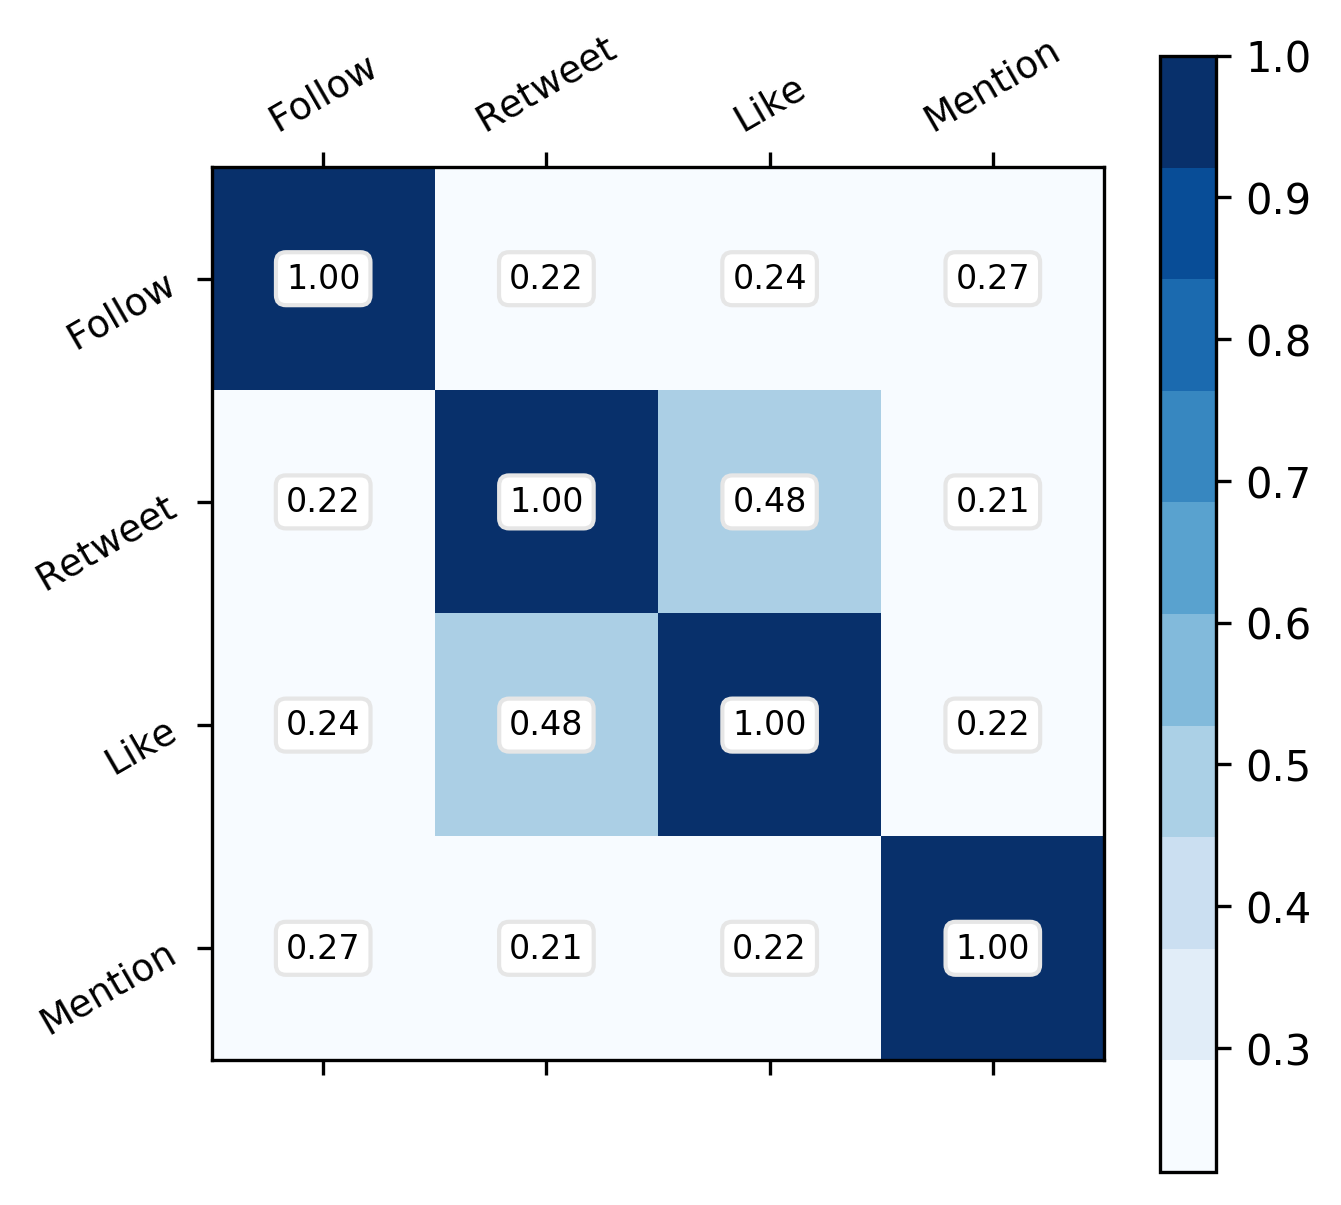
\includegraphics[width=0.45\textwidth]{fig/net_struct/rbo/rbo_in_degree_rank.png}
        \label{fig:rbo_indegree}
    }
    \subfigure[Closeness centrality ranks]{
        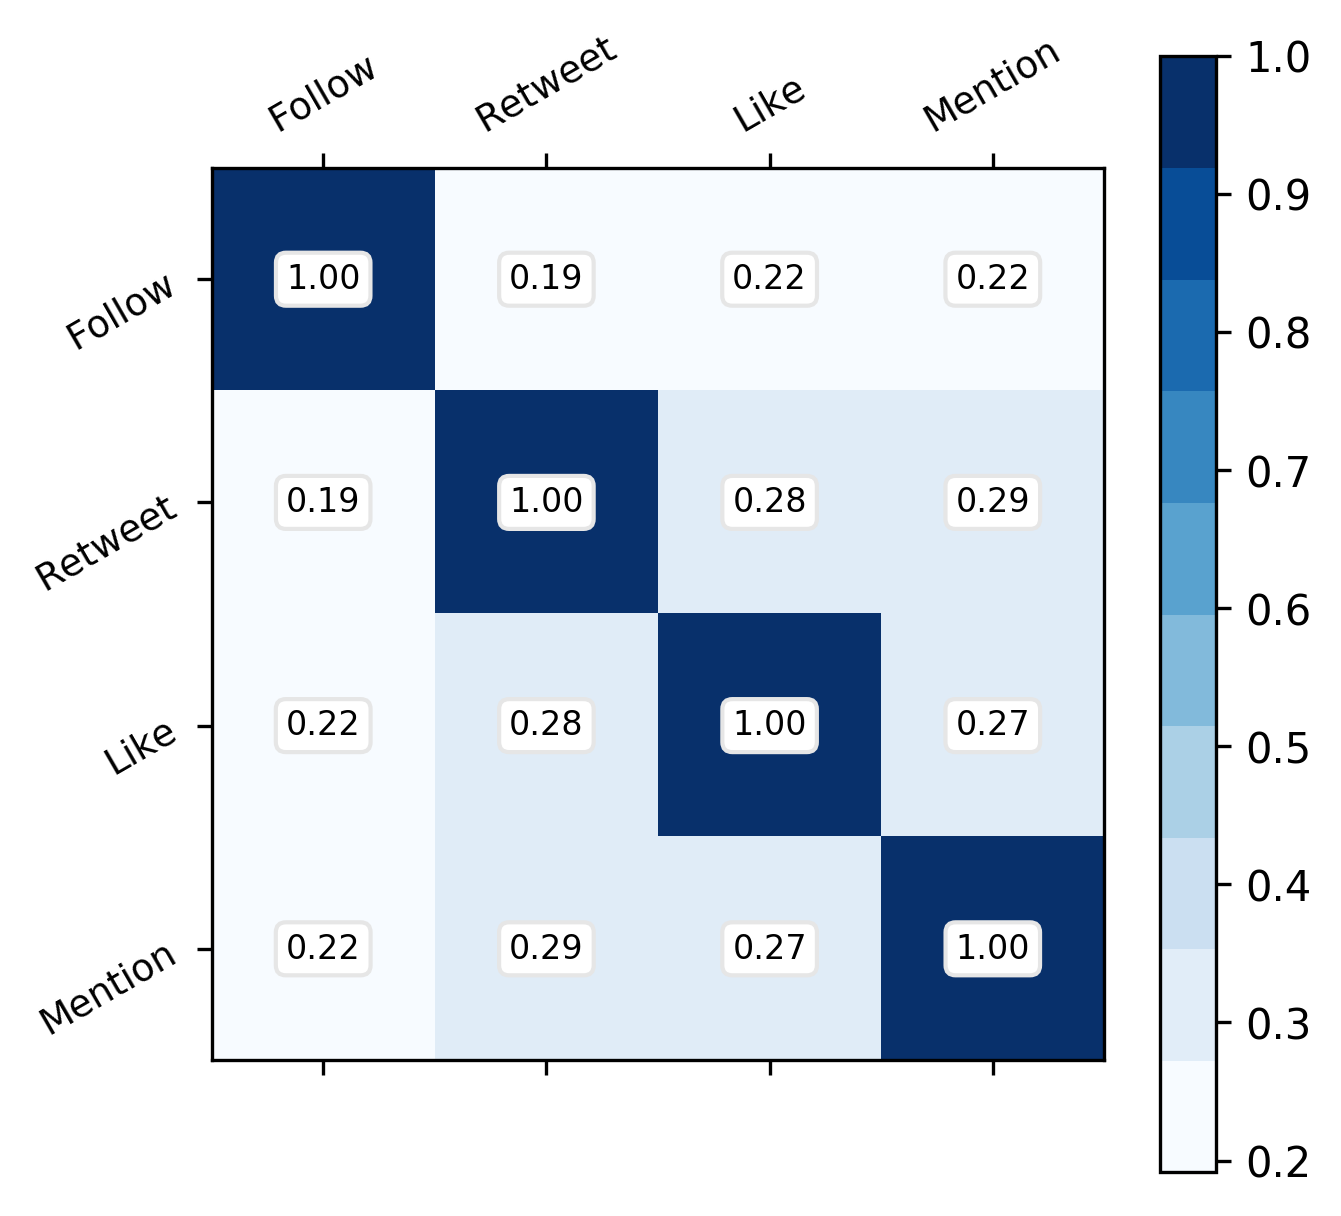
\includegraphics[width=0.45\textwidth]{fig/net_struct/rbo/rbo_close_centr.png}
        \label{fig:rbo_close_centr}
    }
    \caption{Results of extended RBO measure.}
    \label{fig:net_struct_rbo}
\end{figure}

\begin{table}[htb]
\caption{Extended RBO statistics for each pair of layers.}
\label{tab:rbo_statistics}
\centering
\scriptsize
\setlength\tabcolsep{6pt} % default value: 6pt
\begin{tabular}{|l|c|c|}
\hline 
%{{\bf Layer pair}}  &   {{\bf In-Degree Ranks}} &   {{\bf Close Centr. Ranks}} \\ \hline
\multicolumn{1}{|c|}{\textbf{Layer Pair}} & \multicolumn{1}{|c|}{\textbf{In-Degree Ranks}} & \multicolumn{1}{|c|}{\textbf{Close Centr. Ranks}} \\ \hline
\hline \hline
{Follow-Retweets}   &       0.22$\pm$0.14       &       0.19$\pm$0.10           \\ \hline
{Follow-Likes}      &       0.24$\pm$0.14       &       0.22$\pm$0.12           \\ \hline
{Follow-Mentions}   &       0.27$\pm$0.16       &       0.22$\pm$0.14           \\ \hline
{Retweets-Likes}    &       0.48$\pm$0.20       &       0.28$\pm$0.11           \\ \hline
{Retweets-Mentions} &       0.21$\pm$0.13       &       0.29$\pm$0.11           \\ \hline
{Likes-Mentions}    &       0.22$\pm$0.14       &       0.27$\pm$0.11           \\ \hline
\hline
\end{tabular}
\end{table}

We compared the rankings of vertices according to indegree and closeness centrality using the Extended RBO similarity measure discussed in Section \ref{subsec:rbo}. The mean values of Extend RBO are shown in Fig. \ref{fig:net_struct_rbo} for $p=0.98$, which implies that the top 50 vertices having about 86\% of the weight in the evaluation of the overlap between the rankings. Figure \ref{fig:rbo_indegree} shows that there is around 21\% to 27\% overlap among the 50 vertices with highest indegree values in every pair of layers, except for the pair (retweet, like), with a mean overlap of almost 50\%. The great similarity between these two rankings, may be explained by the fact that both interactions  are used to express that a tweet was considered interesting by the person who is the agent of the interactions. Because it is a mean in each pair of layers for the 500 multilayer ego networks, we enter the statistical details in the Table \ref{tab:rbo_statistics}.

The existence of intersection between the top ranked vertices in two layers is a relevant information because it shows that there are hubs (vertices with high indegree values) in at least two distinct layers. These layer-pair-wise hubs may be useful in Twitter applications related to information diffusion, since they are influential vertices in more than one type of interaction and they could, at least hypothetically, help disseminate information through the whole ego network (the composed of the union  of vertices and edges of all layers). 



%%%%%%%%%%%%%%%%%%%%%%%%%%%%%%%%%%%%%%%%%%%%%% 
%%%%%%%%%%%%%%%%%%%%%%%%%%%%%%%%%%%%%%%%%%%%%% Top-k Alters Overlap
\subsection*{Top-k Alters Overlap}
\label{subsec:topk_overlap}

We also investigated in the case of the retweet, like and mention layers if the alters with whom the ego interacts most also are her alters in the other layers. In these three layers, the ego $e$ can interact many times with a same alter $a$, by retweeting or liking many tweets authored by $a$, or by mentioning $a$ in many tweets. For the follow layer this is not the case, since the follow interaction occurs only once. To measure how many of the most interacted alters in layer $x$ were also present in other layer $z$, we first obtained the set $Top_e^x$ which is formed by the $k$ alters with whom the ego $e$ interacted most by type of interaction $x$. Next we computed fraction of elements in $Top_e^x$ that  were also in  $A_e^z$, as: $r(A_e ^z,Top_e^x) =\frac{|A_e^z \cap Top_e^x|}{k}$.

\begin{figure}[h!tb]
    \centering
    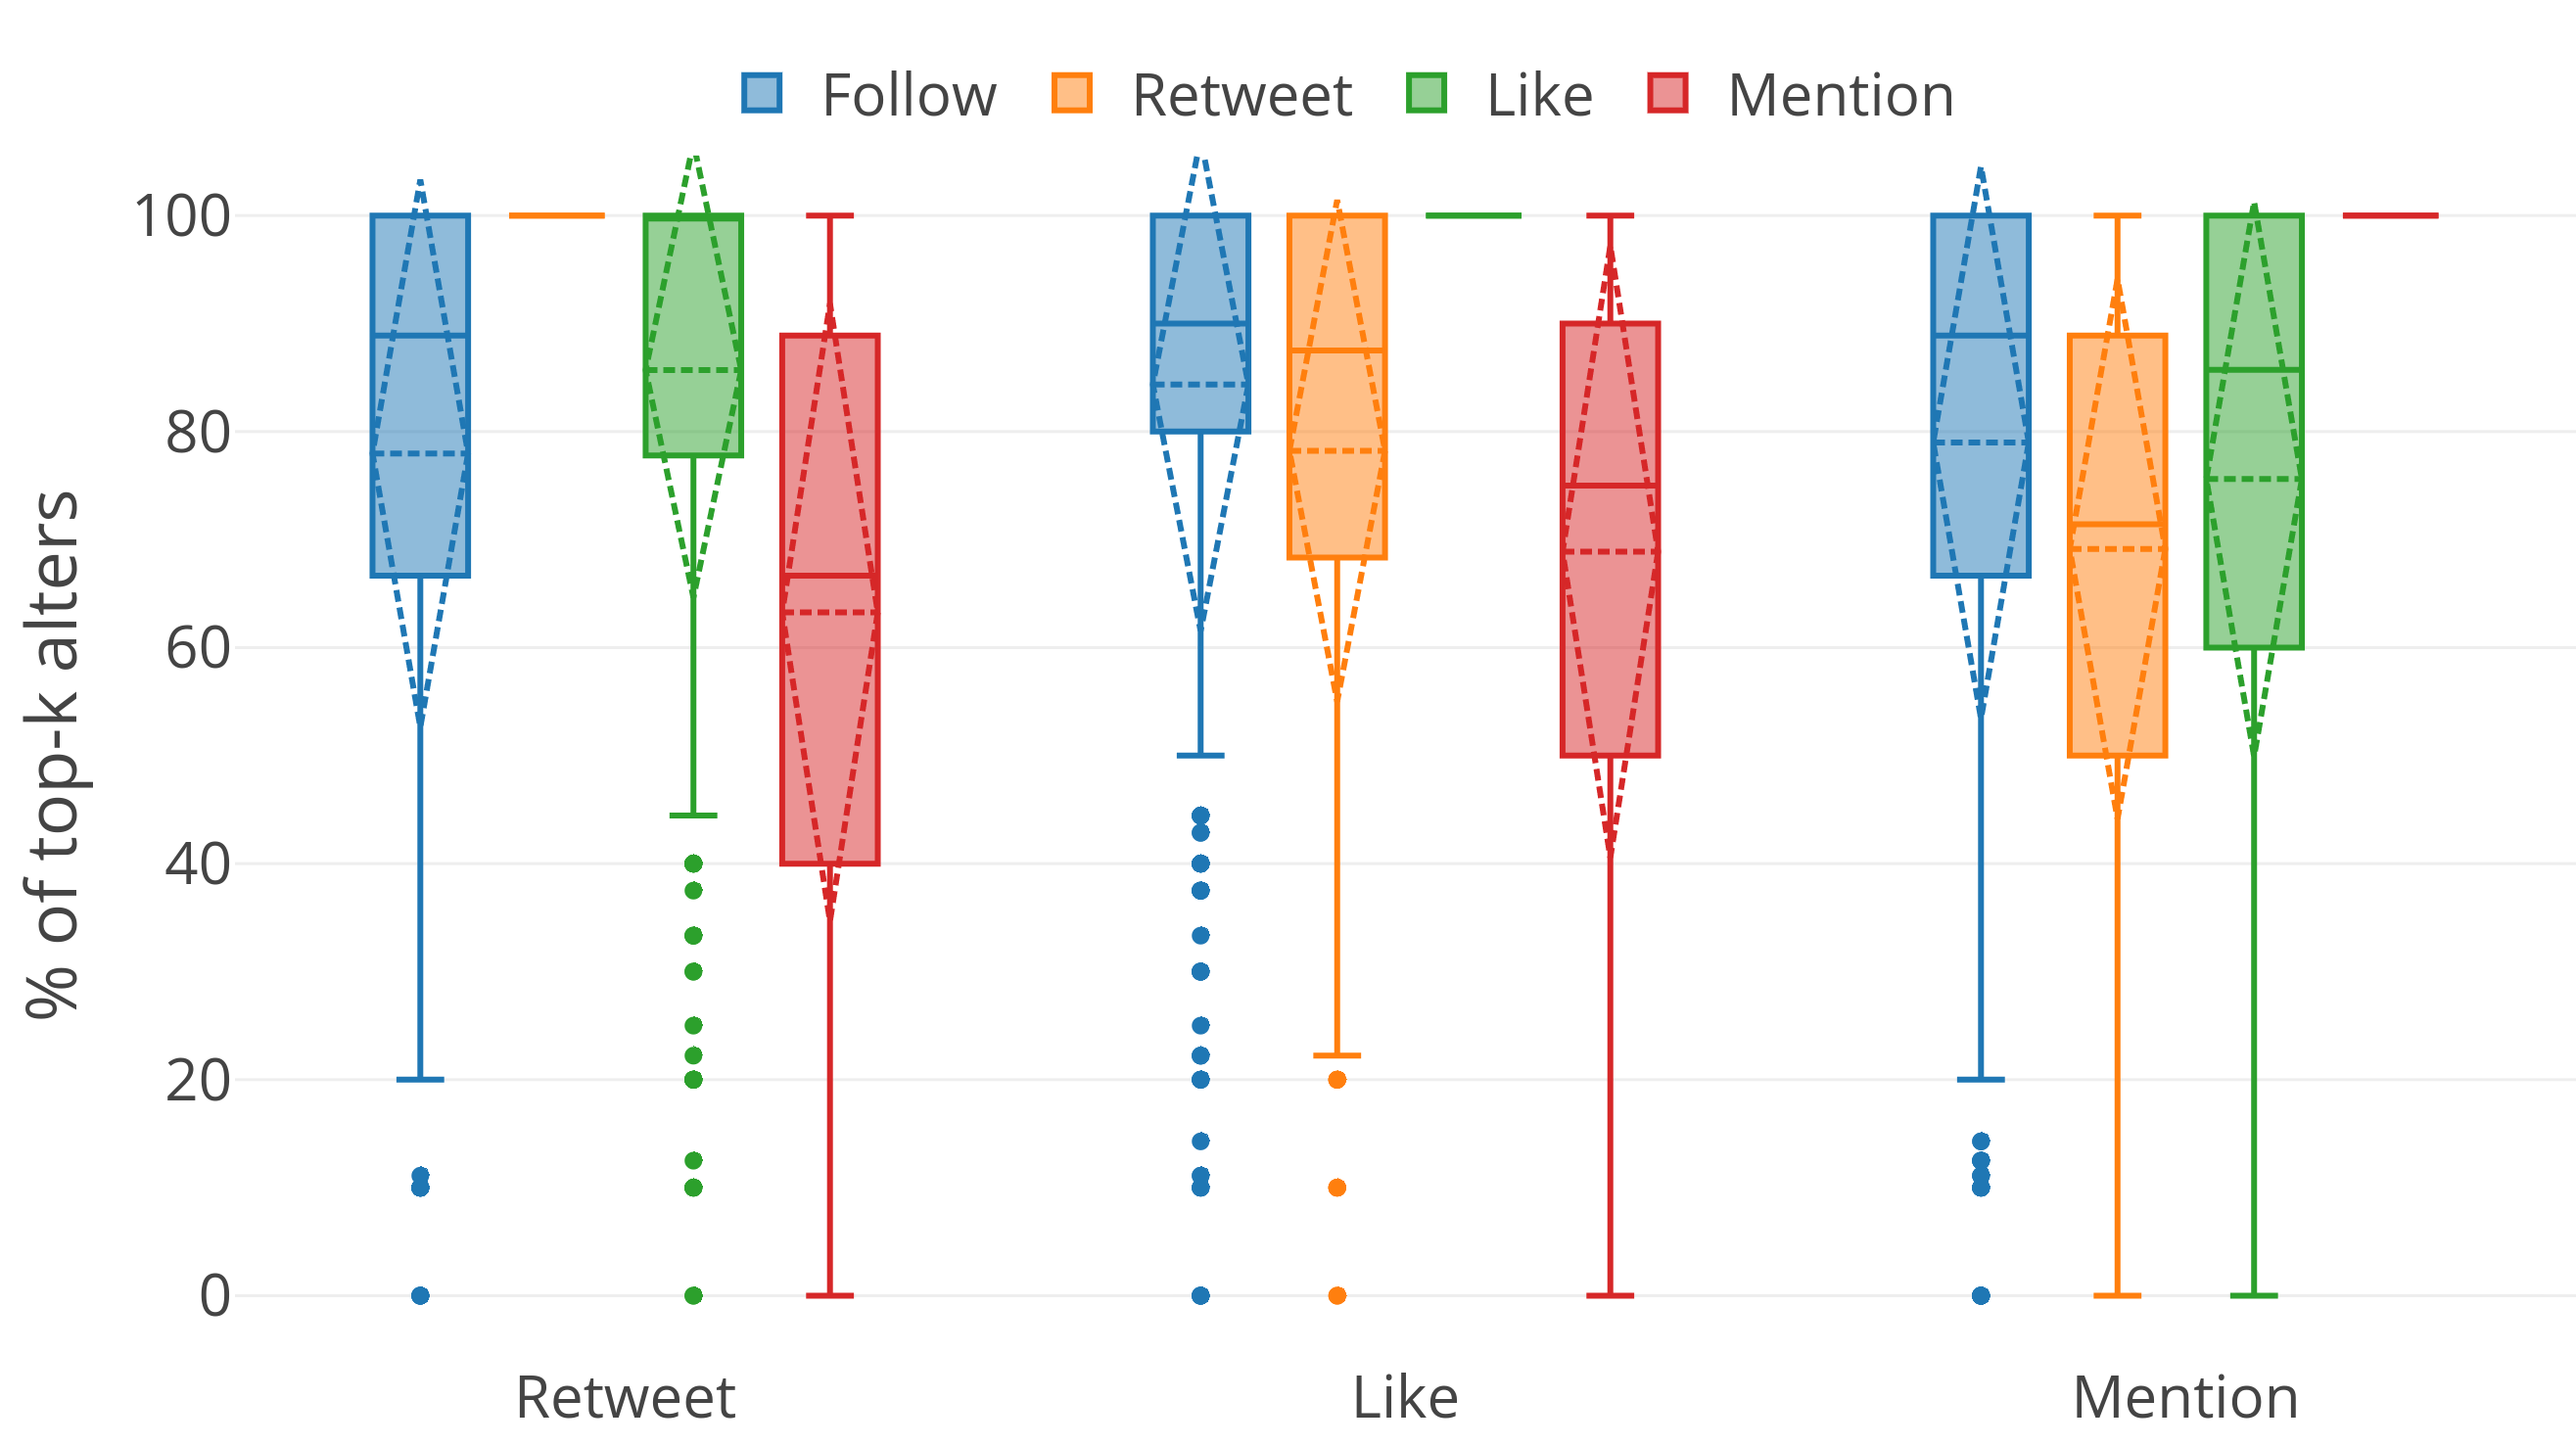
\includegraphics[width=1\textwidth]{fig/net_struct/topk_co_occurrence_boxplot.png}
    \caption{Percentage of the top-k alters of a layer that appear in the set of alters of the other layers.}
    \label{fig:net_struct_topk_over_alters}
\end{figure}

Figure \ref{fig:net_struct_topk_over_alters} shows results of this ratio for $x \in\{reteet, like, mention \}$, for $k=10$. For each layer (x axis), Fig. \ref{fig:net_struct_topk_over_alters} shows four box plots representing the distribution of $r(A_e ^z,Top_e^x)$, for $z \in\{follow,like, retweet, mention\}$. The results shows that there is also a great variability on the values of $r(A_e ^z,Top_e^x)$, with some egos having no alter in $Top_e^x$ occurring in another alter set $A_e^x$ and some egos where the all elements in $Top_e^x$ occurring in another alter set. For most egos the ratio values are high, but it is clear from the figure that the top 10 alters most interacted with by the retweet and like interaction are the ones that occur less in the mention layer, contributing to reinforce lack of affinity between the like and mention interaction and also between the retweet and mention interactions. Besides, we can observe more affinity between the retweet and like layers with most egos having the top 10 alters in one of these layers also being alters in the other layer. 

We find that the for all the tree layers (retweet, like and mention) the top 10 alters in these layers tend to occur frequently in the follow layer. But, it is important to remember that this fact may be due to limitations on the construction of the alter sets reported in Section \ref{cap:ExpSetup}, with the alter set for the follow layer being bigger than the alter set of the remaining layers for most egos. Despite the high values of the ratio regarding the follow layer, the blue box plots in Figure \ref{fig:net_struct_topk_over_alters} reveal an interesting problem: {\em many users may not receive all the tweets produced by the alters they interact most with retweets, likes and mentions}. As the box plots show, for about 25\% of the egos, their most retweeted alters are not followed by them, and 50\% of egos do not follow 20\% of their most retweeted alters (left most blue box plot in the figure). A similar situation can be seen with the most mentioned alters (rightmost blue box plot).

The miss of tweets coming from this most preferable alters may occur because the egos do not follow these alters. When a user $e$ follows another user $a$ in Twitter, all the tweets authored or retweeted by $a$ are propagated to $e$’s  timeline. If $e$ does not follow $a$, $e$ receives a tweet retweeted or authored by $a$ only if another user followed by $e$ retweets this tweet. This implies that if a tweet produced or retweet by $a$ may not reach $e$’s timeline if none of the followees of $e$ retweet it. In this case, $e$ may be missing information produced by her most preferable tweet producers. 

When considering the retweet interaction, the above problem may have another implication: if a tweet authored by a preferable alter regarding the retweet interaction is not delivered in the ego’s timeline the tweet loses a great chance to be propagated in the network by an ego with a great probability of retweeting it, affecting information cascading in Twitter. The above problem may be diminished by recommending to a user to follow people to whom they interact most by retweets, likes and mention and who she is not following yet. Twitter has a user recommendation service, but it not known if the service suggests the type of recommendation just mentioned above.



%%%%%%%%%%%%%%%%%%%%%%%%%%%%%%%%%%%%%%%%%%%%%% 
%%%%%%%%%%%%%%%%%%%%%%%%%%%%%%%%%%%%%%%%%%%%%% 



\section{Do the indegree distributions follow a power-law?}
\label{sec:QuestionPowerLaw}

\begin{figure}[h!tb]
    \centering
    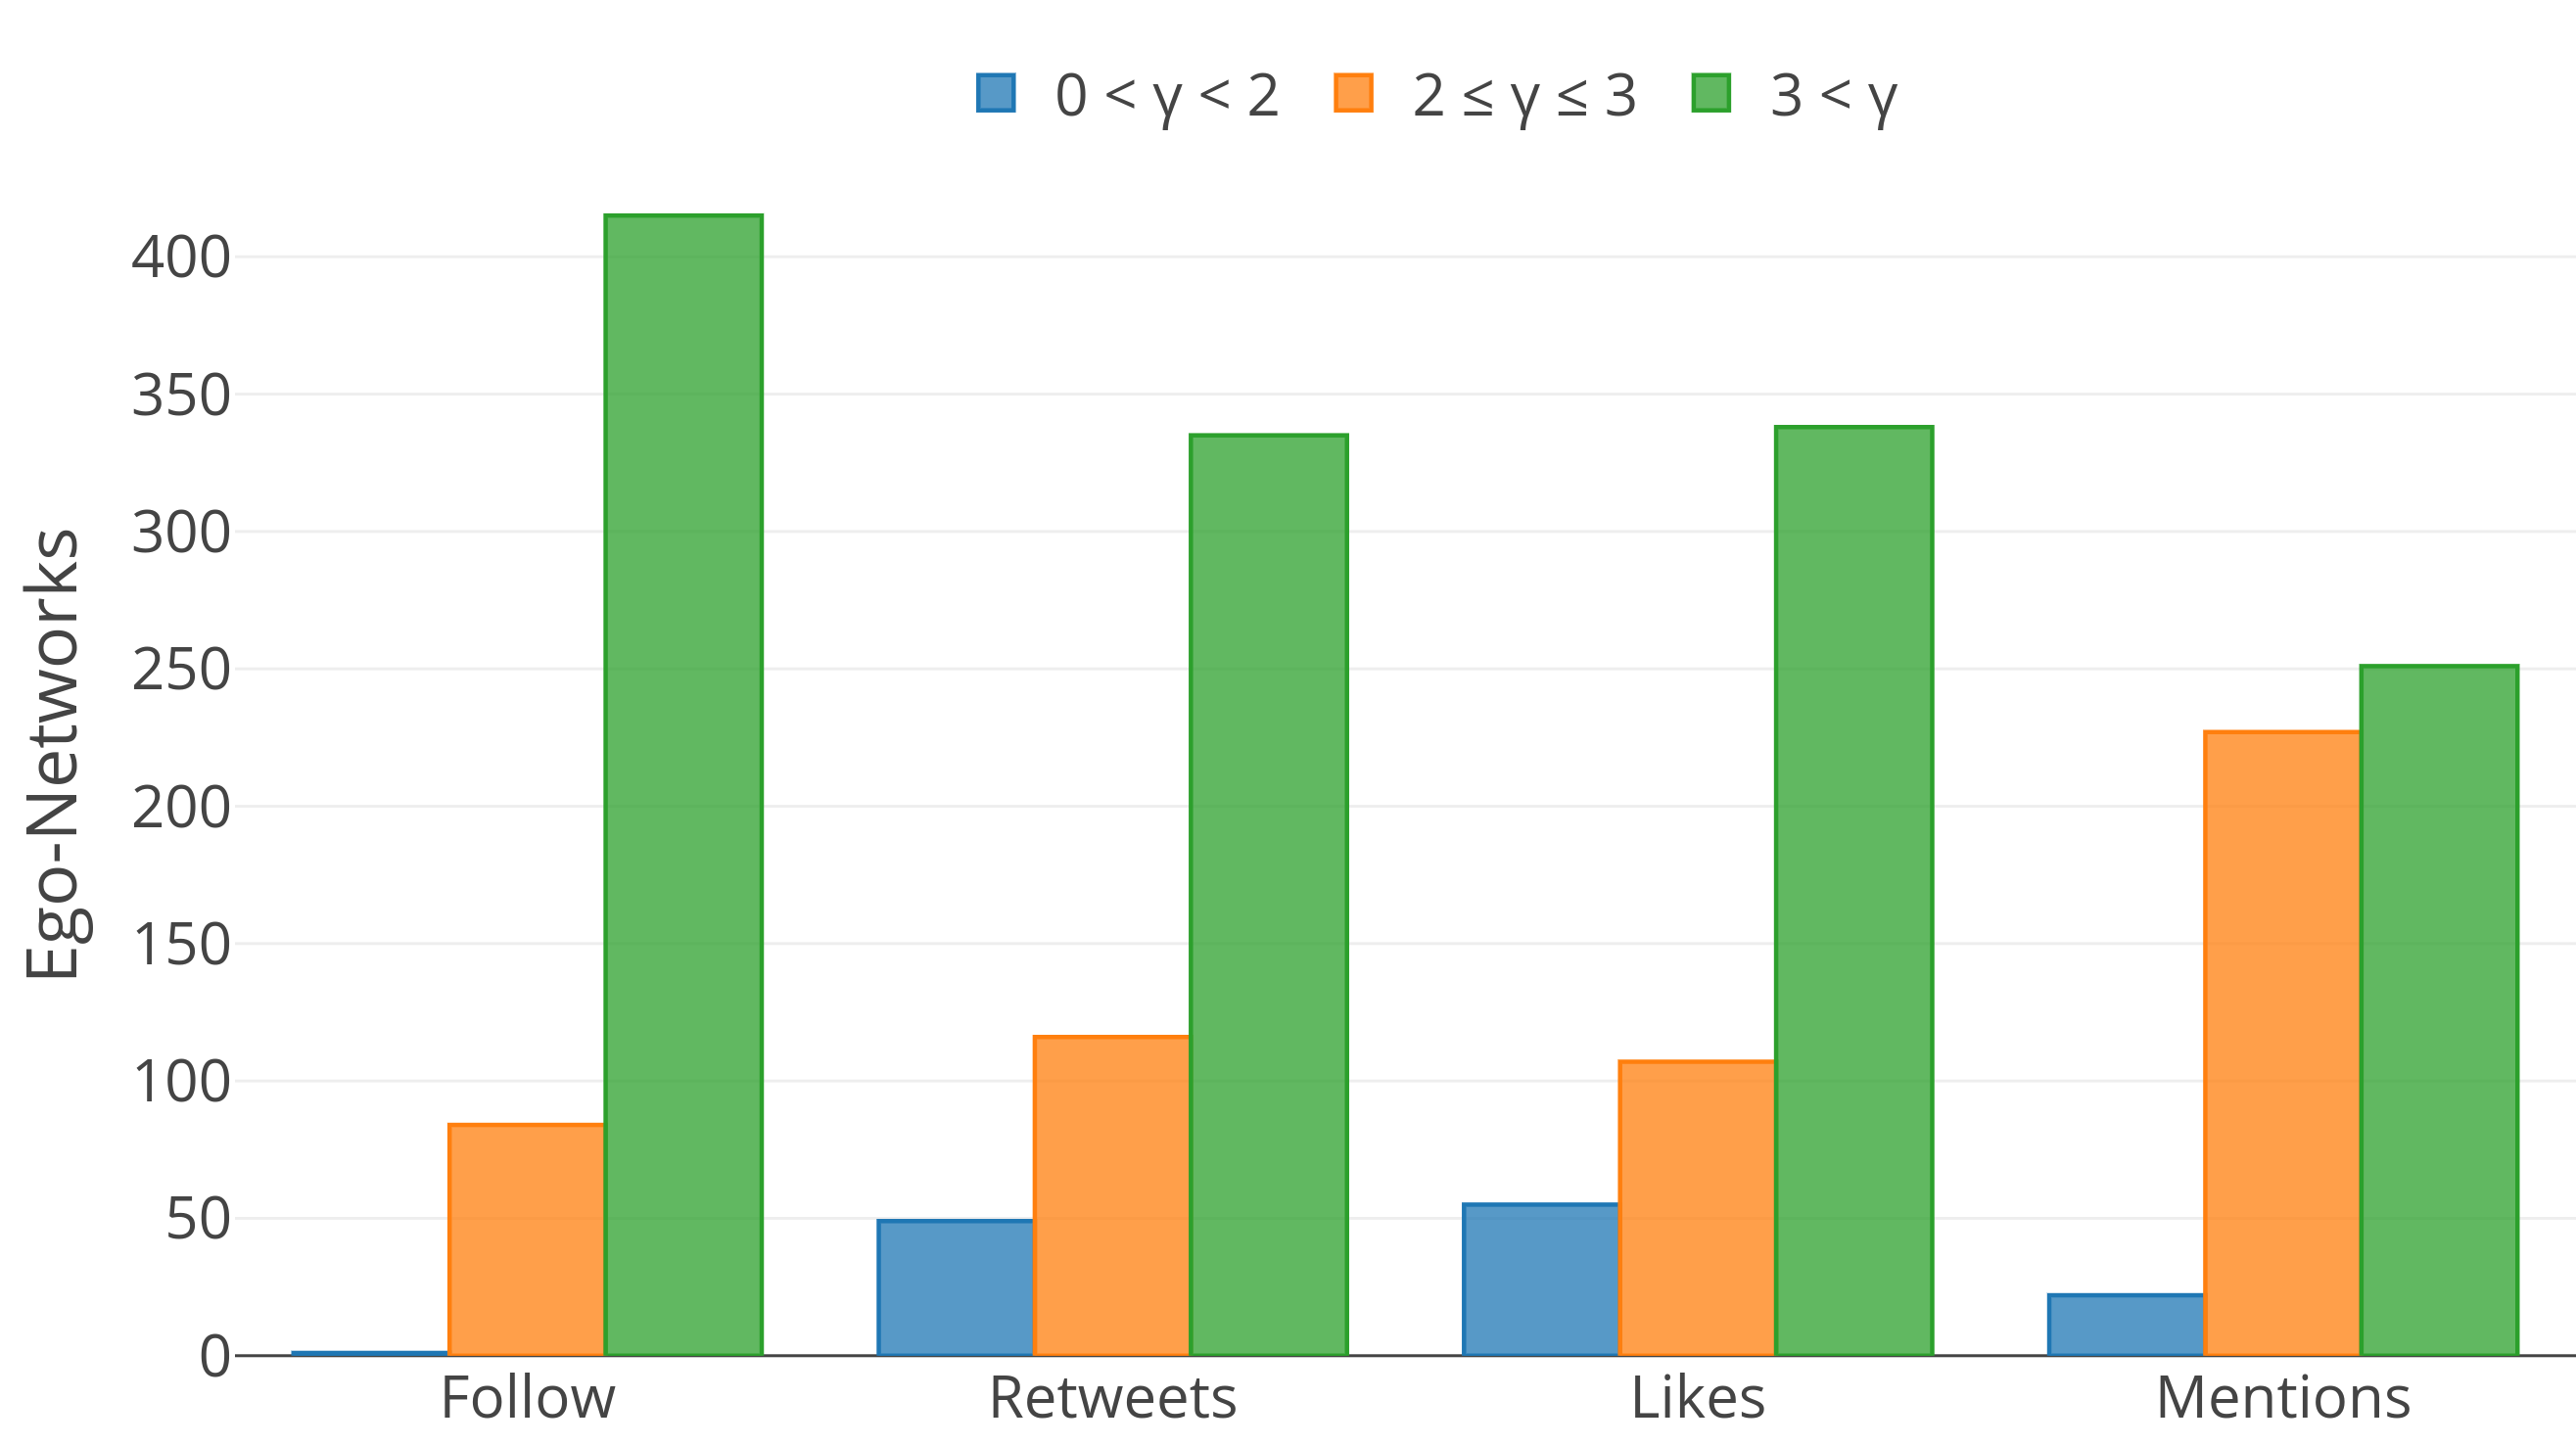
\includegraphics[width=1\textwidth]{fig/net_struct/in_degree_distribution.png}
    \caption{Classification of the ego networks as to the distribution of the indegree.}
    \label{fig:net_struct_indegree_distribution}
\end{figure}

We verifyied if the the indegree distributions in all layers followed a power-law, i.e., if they could be described by Eq. \ref{eq:1}. We used the Powerlaw Python package \cite{Alstott2014} to find the appropriate functions to fit the data. We found that indegree distributions in all layers follow a power-law, but as happens with all the other aspects analyzed, there is great variation on the results. Diverse variations of $\gamma$ values we found. We classified the distributions in three categories: Category A with $0<\gamma <2$; Category B, with $2<\gamma<3$ and Category C, with $\gamma> 3$. This categorization was used because most networks found in nature and those derived from human activities are known to follow a power-law with $2<\gamma<3$, i.e., belong to Category B. Thus, we adopted the interval corresponding to Category B to separate layers  that fit a “standard power-law” (Category B) from those that are apart from the standard, with inferior $\gamma$ values (Category A) or superior $\gamma$ values (Category C).

Figure \ref{fig:net_struct_indegree_distribution} shows the distribution of categories found in each layer. Despite the existence of very different $\gamma$ values, for most egos, the indegree distribution in the follow, retweet and like layers follow a power-law distribution of Category C. The mention layer is the one that most approaches what we refer to “standard power-law” regarding  the indegree distributions, since the number of egos whose mention layers fallow in Category B is the largest, comparing to the other layers. The consequence of these observations is that for the great majority of egos we have in all layers  very few alters who are the target of many interactions originated from the other alters or form the ego. On the other hand, the great majority of alters (the long tail) receive very few interactions in the layers. 



%%%%%%%%%%%%%%%%%%%%%%%%%%%%%%%%%%%%%%%%%%%%%% 
%%%%%%%%%%%%%%%%%%%%%%%%%%%%%%%%%%%%%%%%%%%%%% 



\section{Are the layers small-world graphs?}
\label{sec:QuestionSmallWorld}

We analyze whether each layer of multilayer ego networks can be classified as small-worlds. For this we use the definition presented in section \ref{sec:small_worlds}, which uses a trade-off between clustering coefficient and average shortest path length (ASPL), comparing them with an equivalent random graph, with the same number of vertices and edges. The clustering coefficient was calculated using the formula described in Eq. \ref{eq:locClustCoef}, and the ASPL was calculated as described in \cite{Mao2013}, which uses the ratio of the sum of all minimum paths between all vertices about the number of existing shortest paths, according to Eq. \ref{eq:ASPL}.

\begin{figure}[h!tb]
    \centering
    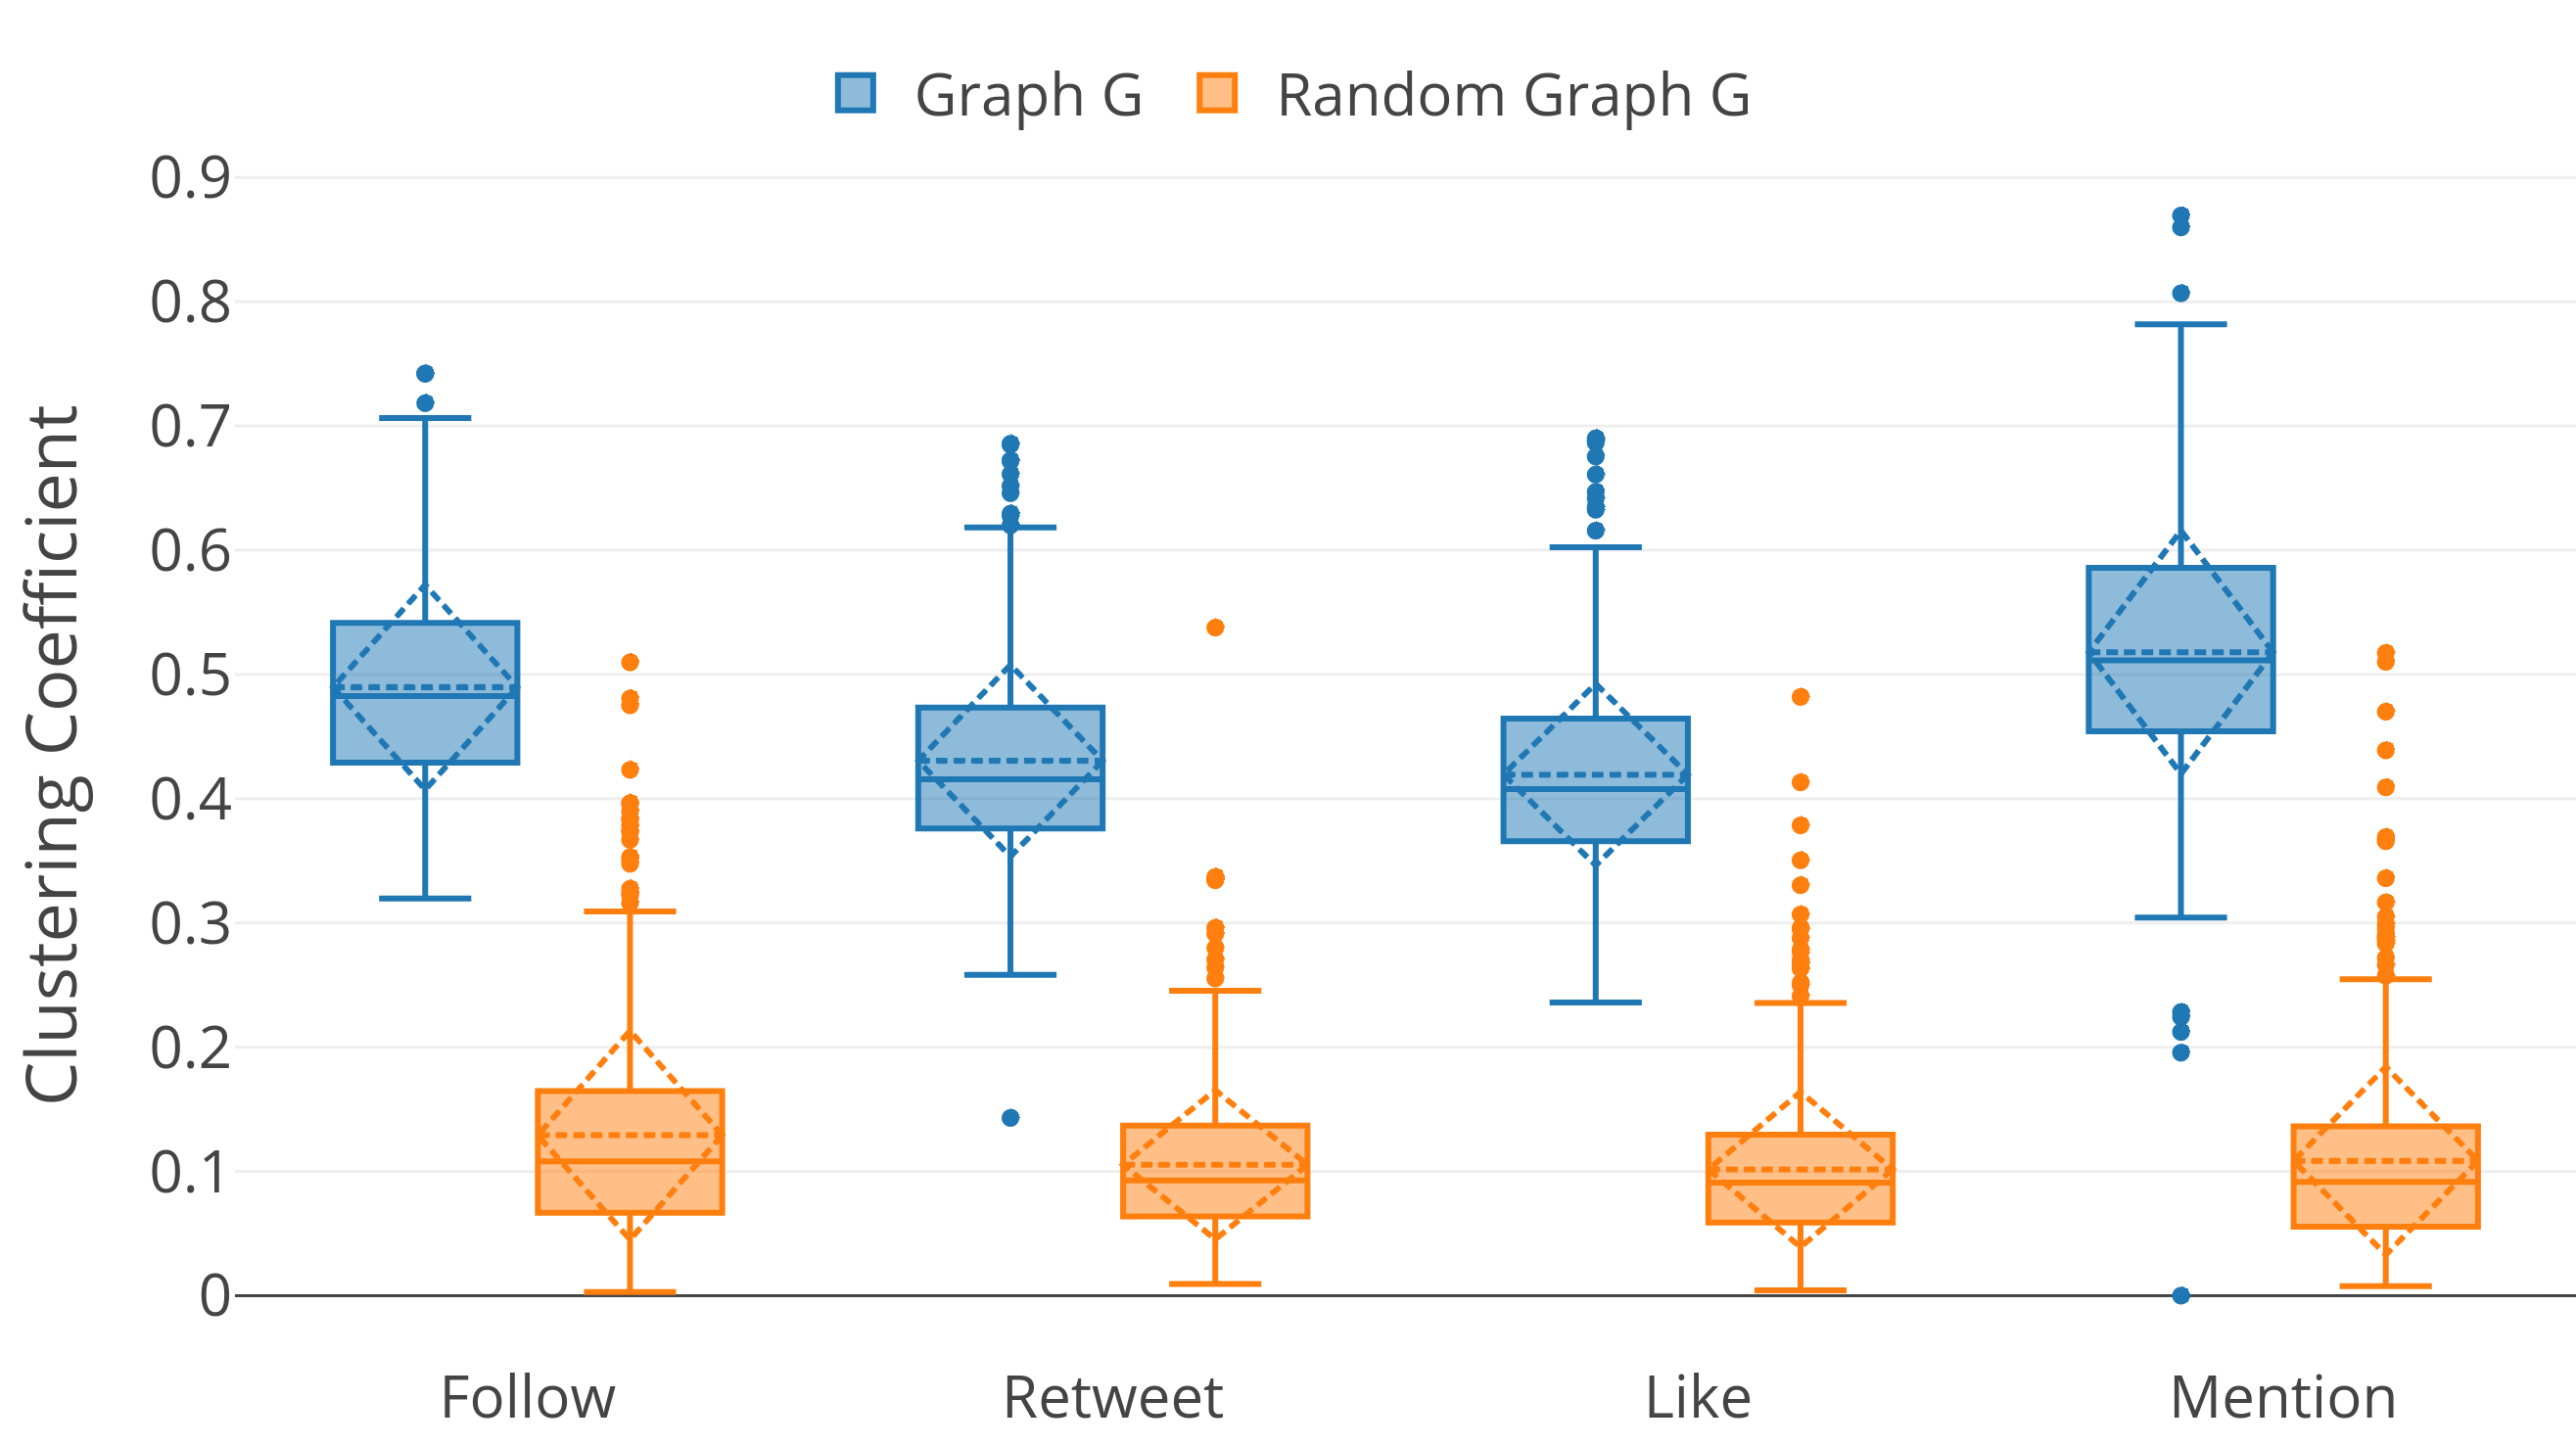
\includegraphics[width=1\textwidth]{fig/net_struct/coef_clust_rnd_g.png}
    \caption{Clustering coefficient of graph G and random graph G.}
    \label{fig:net_struct_coef_clust_rnd_g}
\end{figure}

\begin{figure}[h!tb]
    \centering
    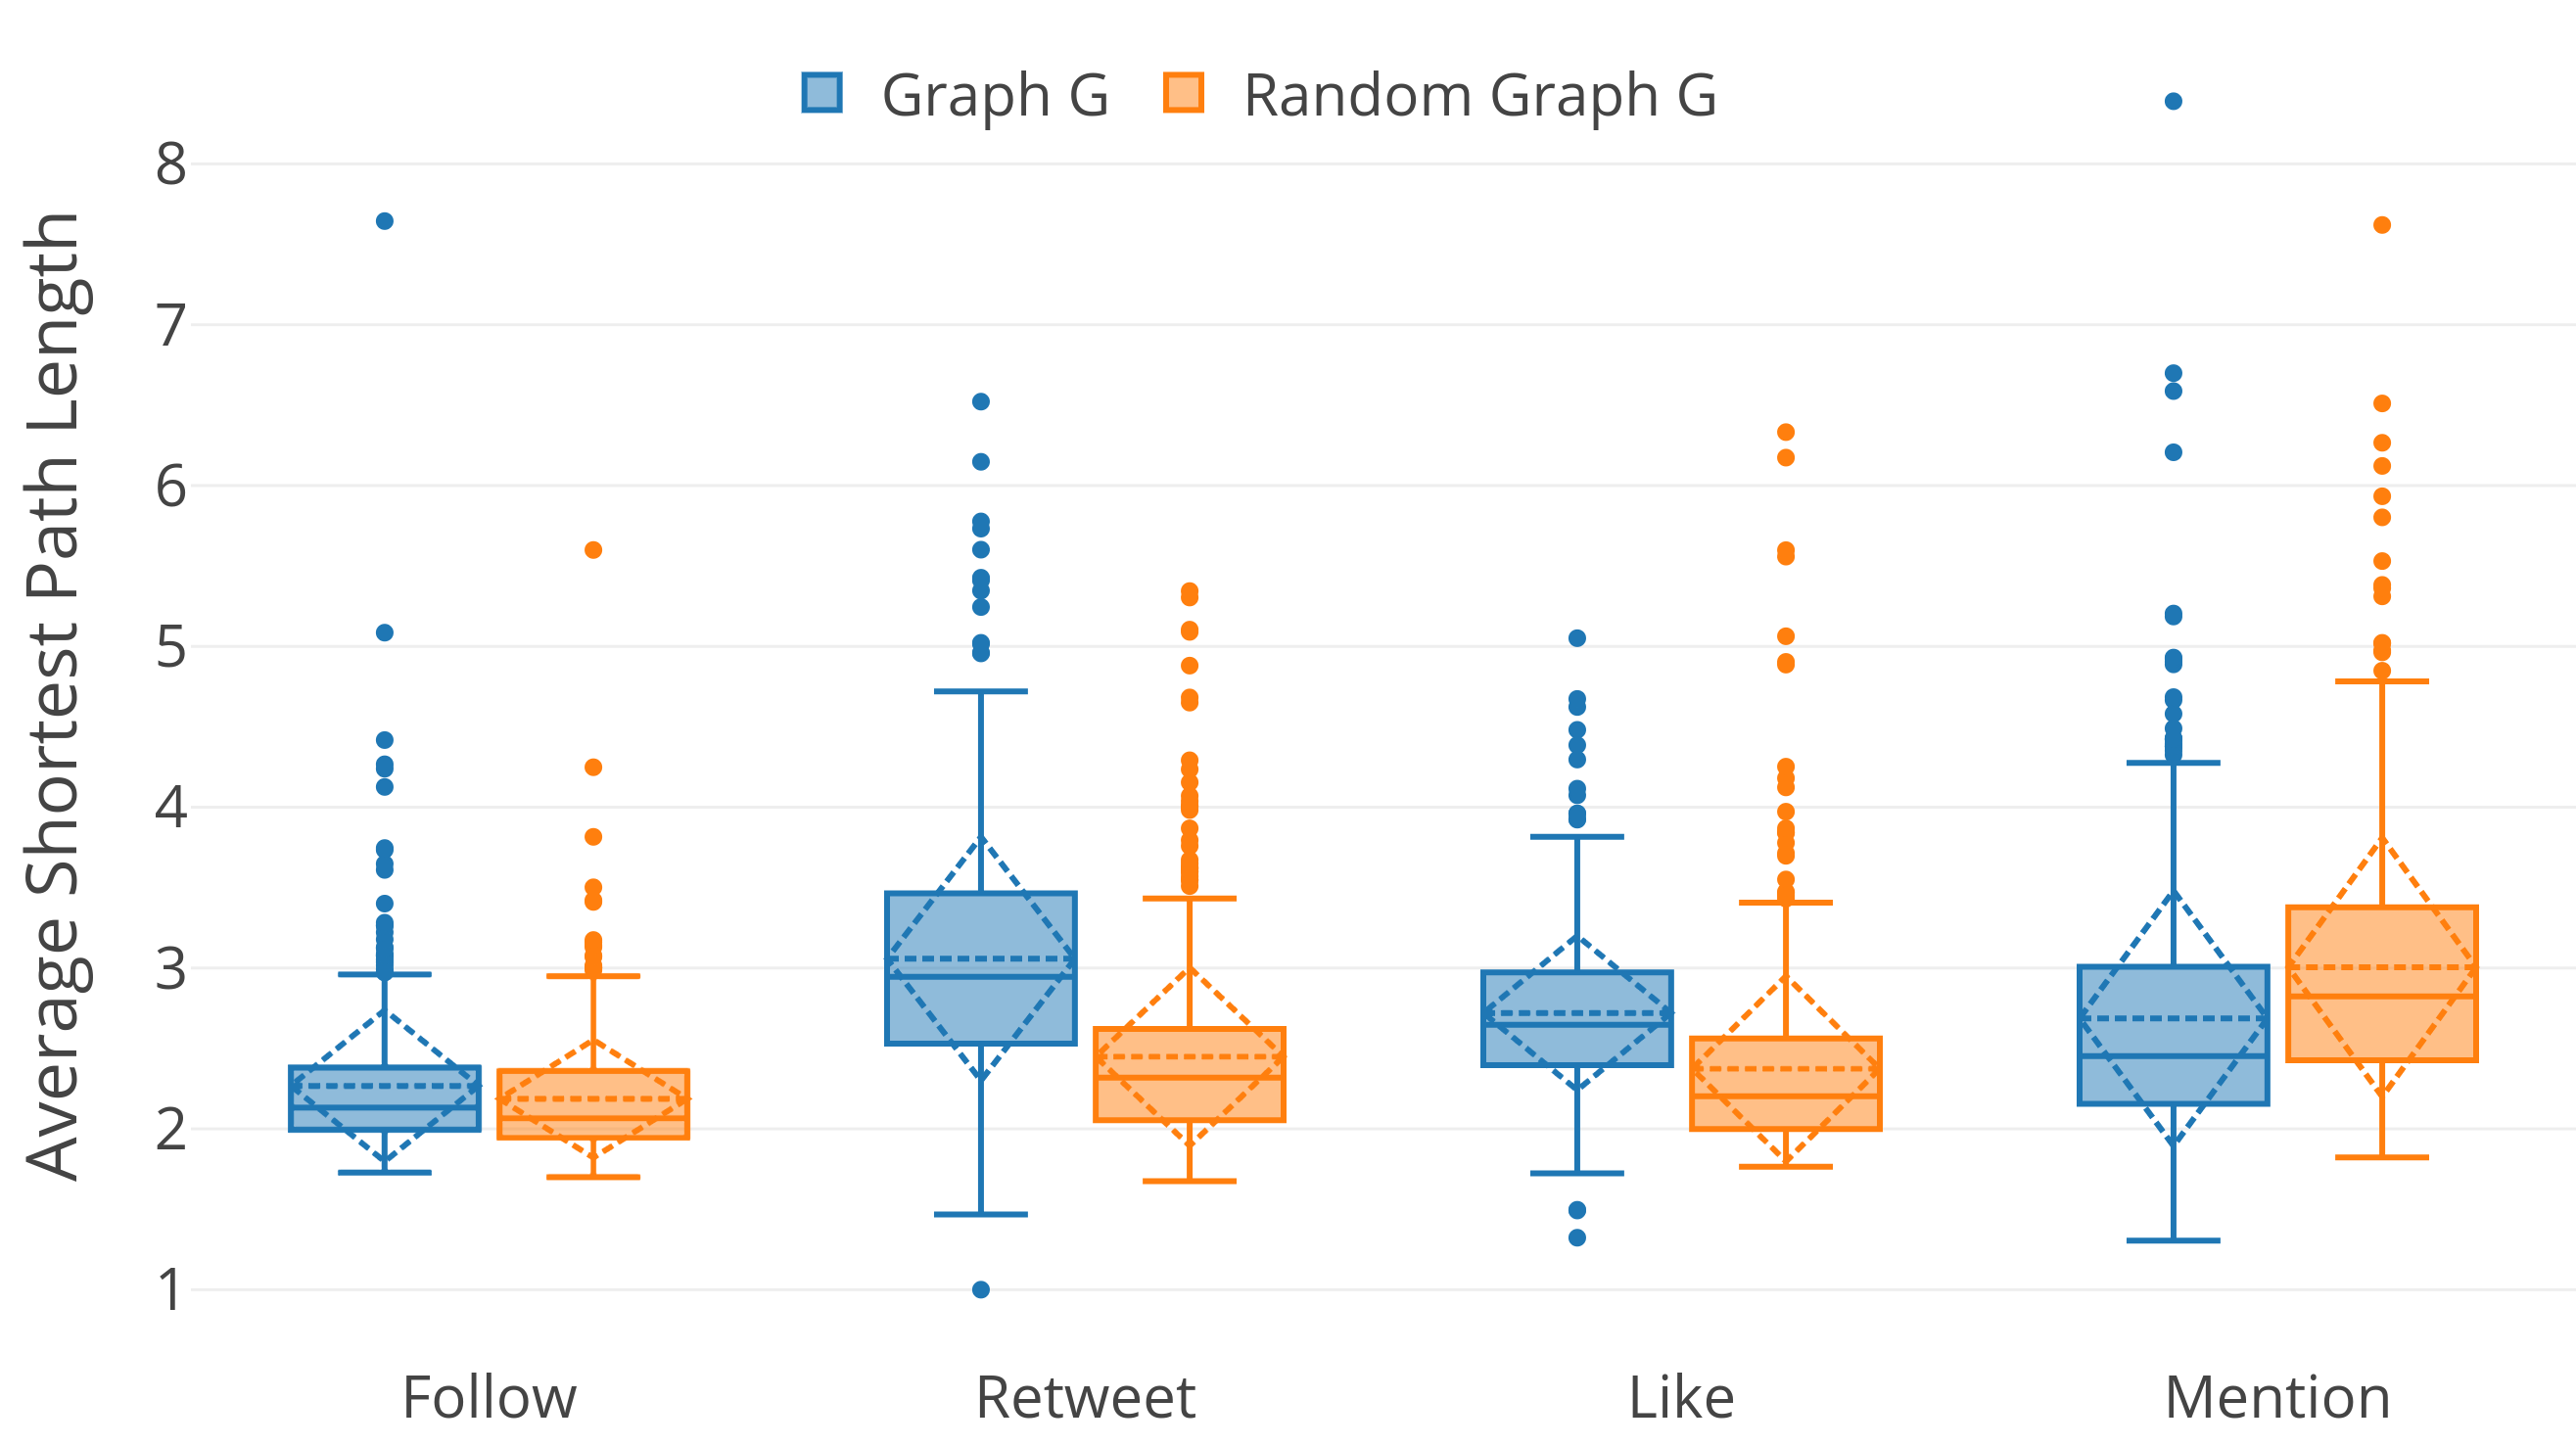
\includegraphics[width=1\textwidth]{fig/net_struct/aspl_rnd_g.png}
    \caption{Average shortest path length of graph G and random graph G.}
    \label{fig:net_struct_aspl_rnd_g}
\end{figure}


The Fig. \ref{fig:net_struct_coef_clust_rnd_g} presents the results of the average of the local clustering coefficient of each graph in each layer, and an equivalent Erd\"{o}s-R\'{e}nyi (E$-$R) random graph $G_{E-R}$. The results clearly show that all the layers have high coefficients of grouping of the graphs with respect to the equivalent random graph, indicating that the vertices tend to group with their neighbors, forming communities. The  Fig. \ref{fig:net_struct_aspl_rnd_g} presents the results of the calculation of ASPL for each graph and an equivalent Erd\"{o}s-R\'{e}nyi (E$-$R) random graph $G_{E-R}$, in each layer analyzed. The results show that all layers have low ASPL values, with almost all analyzed graphs showing values between 1.5 and 5. For the Retweet and Like layers the ASPL values are on average larger than the random graph; for the Follow layer the ASPL values are very similar to those found in the random graphs, and only the Mentions layer has on average lower ASPL values than the random graph.

With the values found we could classify the ego networks in small worlds using the metric $S$, according to Eq. \ref{eq:S}.The results were arranged in the table \ref{tab:small_world}. We can observe that all 500 graphs of the Follow, Retweet and Like layers obtained values of $S$ greater than 1, and only two graphs in the Mention layer obtained results equal to or lower than 1 for the metric $S$, possibly outliers, as can be observed in the figures \ref{fig:net_struct_coef_clust_rnd_g} and \ref{fig:net_struct_aspl_rnd_g}. These results show that practically all layers have graphs that can be classified as small-worlds.

\begin{table}[h!tb]
    \renewcommand{\arraystretch}{1.3}
    \caption{Number of ego-networks classified in small world according to metric S}
    \label{tab:small_world}
    \centering
    \scriptsize
    \setlength\tabcolsep{6pt} % default value: 6pt
    \begin{tabular}{|c|c|c|}
        \hline
        {\bf Layer} &   {\bf$S \leq 1$} &   {\bf$1 < S$ }\\ \hline \hline
        Follow      &       -       &       500     \\  \hline
        Retweet     &       -       &       500     \\  \hline
        Like        &       -       &       500     \\  \hline
        Mention     &       2       &       498     \\  \hline\hline 
    \end{tabular}
\end{table}

%%%%%%%%%%%%%%%%%%%%%%%%%%%%%%%%%%%%%%%%%%%%%% 
%%%%%%%%%%%%%%%%%%%%%%%%%%%%%%%%%%%%%%%%%%%%%% 


\section{How is each layer structured in communities?}
\label{sec:QuestionCommunities}

%\section{Configuring Community Detection Algorithms}
%\label{sec:exp_alg_comm_detection}
To investigate if layers are organized in communities we applied different community detection algorithms in all layers of all ego networks considered. The algorithms used are described in the Table \ref{tab:CommDetectionAlgs}. These algorithms are widely used in the work of community detection in graphs, so they are already consolidated algorithms, and were selected according to criteria related to computational complexity, application in directed networks, detection capacity of disjoint or overlapping communities - taking into account the realities of OSNs - and availability of software access. Its characteristics have been described in the section \ref{sec:comm_algorithms}.

The COPRA algorithm required a specific parameter ($v$), which determines the maximum number of communities that a vertex can be associated with. As pointed out by Wu et al. \cite{Wu2012}, the choice of parameter $v$ is difficult and induces the non-determinism of COPRA, since, because it is global vertex-independent parameter, it does not take into account that a large number of vertices do not overlap while few vertices participate in many communities. In our experiment we used $v = 2$.  Because COPRA is an extension of the RAK algorithm, running COPRA with $v=1$ causes the RAK algorithm itself to run. Therefore, we use the same code to achieve COPRA and RAK results. For the other algorithms the standard configuration of each was used. 

\begin{table}[h!tb]
   \renewcommand{\arraystretch}{1.3}
    \caption{Algorithms for detecting communities used in experiments.}
    \label{tab:CommDetectionAlgs}
    \centering
    \scriptsize
    \setlength\tabcolsep{6pt} % default value: 6pt
    \begin{tabular}{|c|c|c|c|}
        \hline
		\textbf{Algorithm}              &   \textbf{Type of Community}  & \textbf{Version}  & \textbf{Available in} \\ \hline
		RAK \cite{Raghavan2007}      	&   Disjoint                    & 1.24              & http://gregory.org/research/networks/software \\ \hline
			
		INFOMAP \cite{Rosvall2008}&   Disjoint                    & 0.19.x            & http://www.mapequation.org/code.html \\ \hline
					
		COPRA \cite{Gregory2010}      	&   Overlapping                 & 1.24              & http://gregory.org/research/networks/software \\ \hline
			
		OSLOM \cite{Lancichinetti2011} 	&   Overlapping                 & 2.4               & http://www.oslom.org \\ \hline
			
    \end{tabular}
\end{table}

%To investigate if layers are organized in communities we applied different community detection algorithms in all layers of all ego networks considered. The algorithms used were COPRA \cite{Gregory2010} and OSLOM \cite{Lancichinetti2011} for overlapping communities detecion; and RAK \cite{Raghavan2007} and INFOMAP \cite{Rosvall2008} for disjoint community detection. 


%Número de comunidades detectadas por cada algoritmo
\begin{figure}[h!tb]
    \centering
    \subfigure[Follow]{
        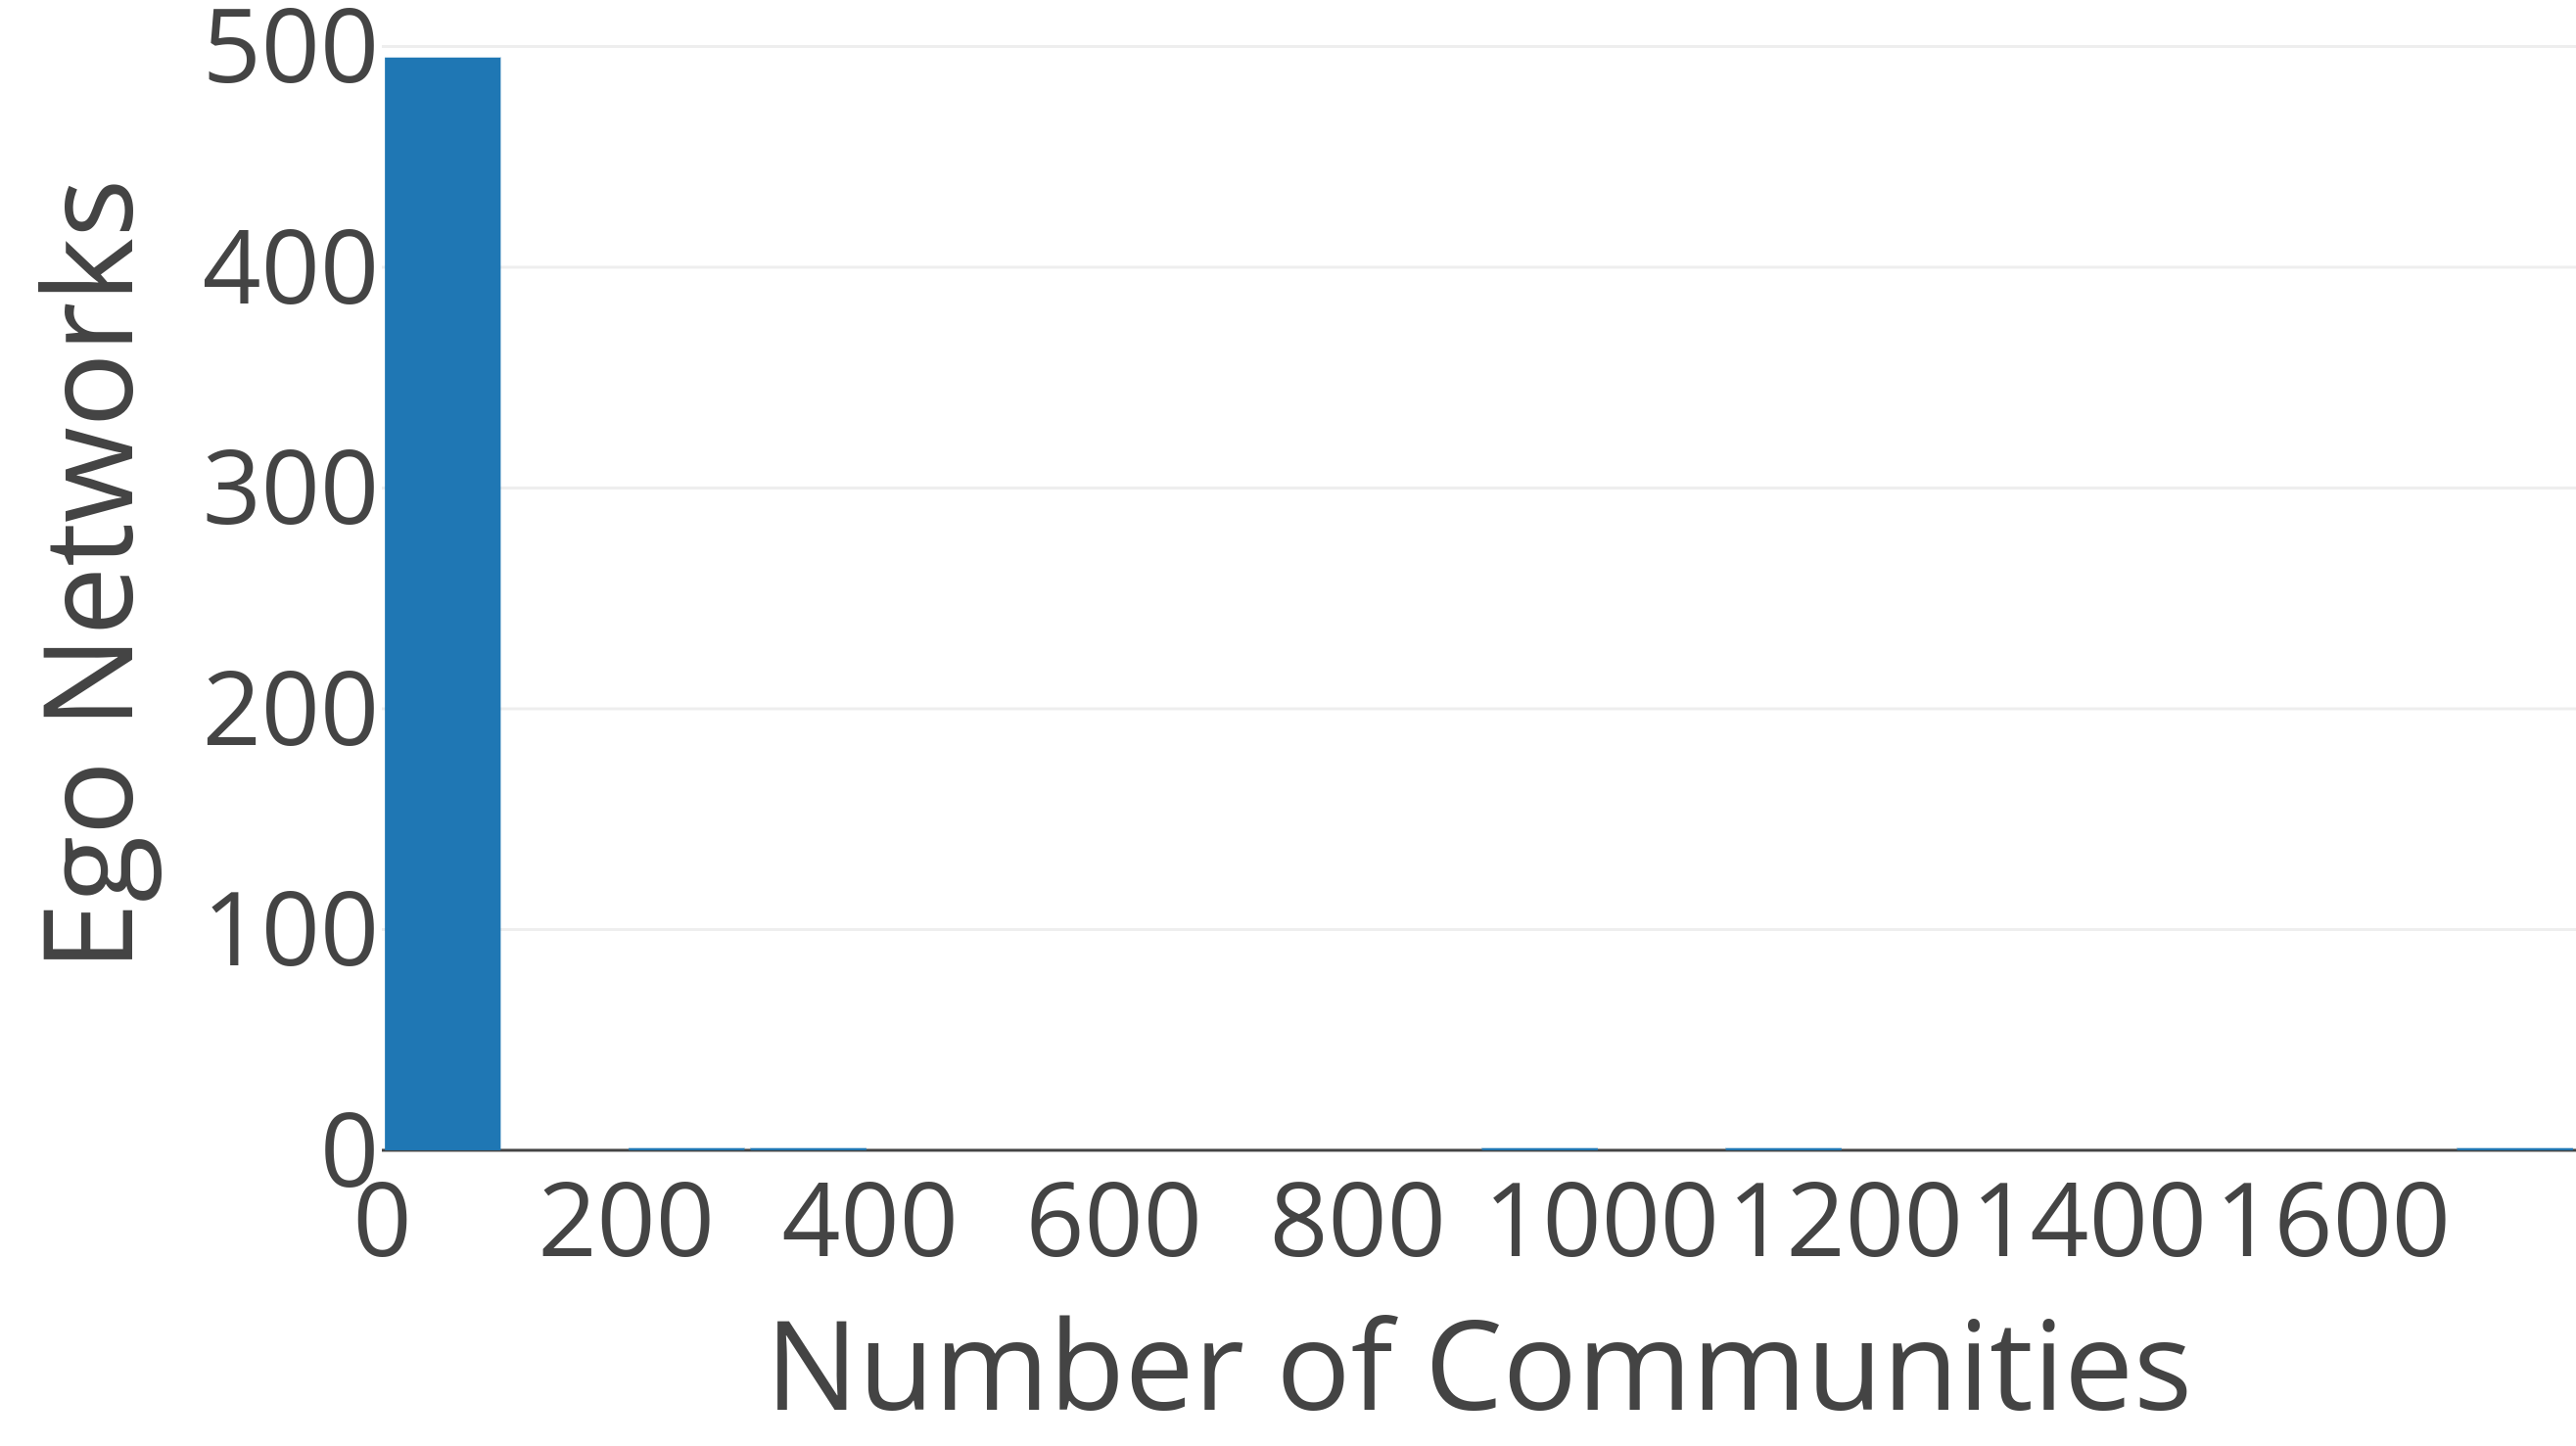
\includegraphics[width=0.47\textwidth]{fig/comm_stats/rak/n_comm/n_comm_rak_follow.png}
        \label{fig:comm_stats_n_comm_rak_follow}
    }
    \subfigure[Retweet]{
        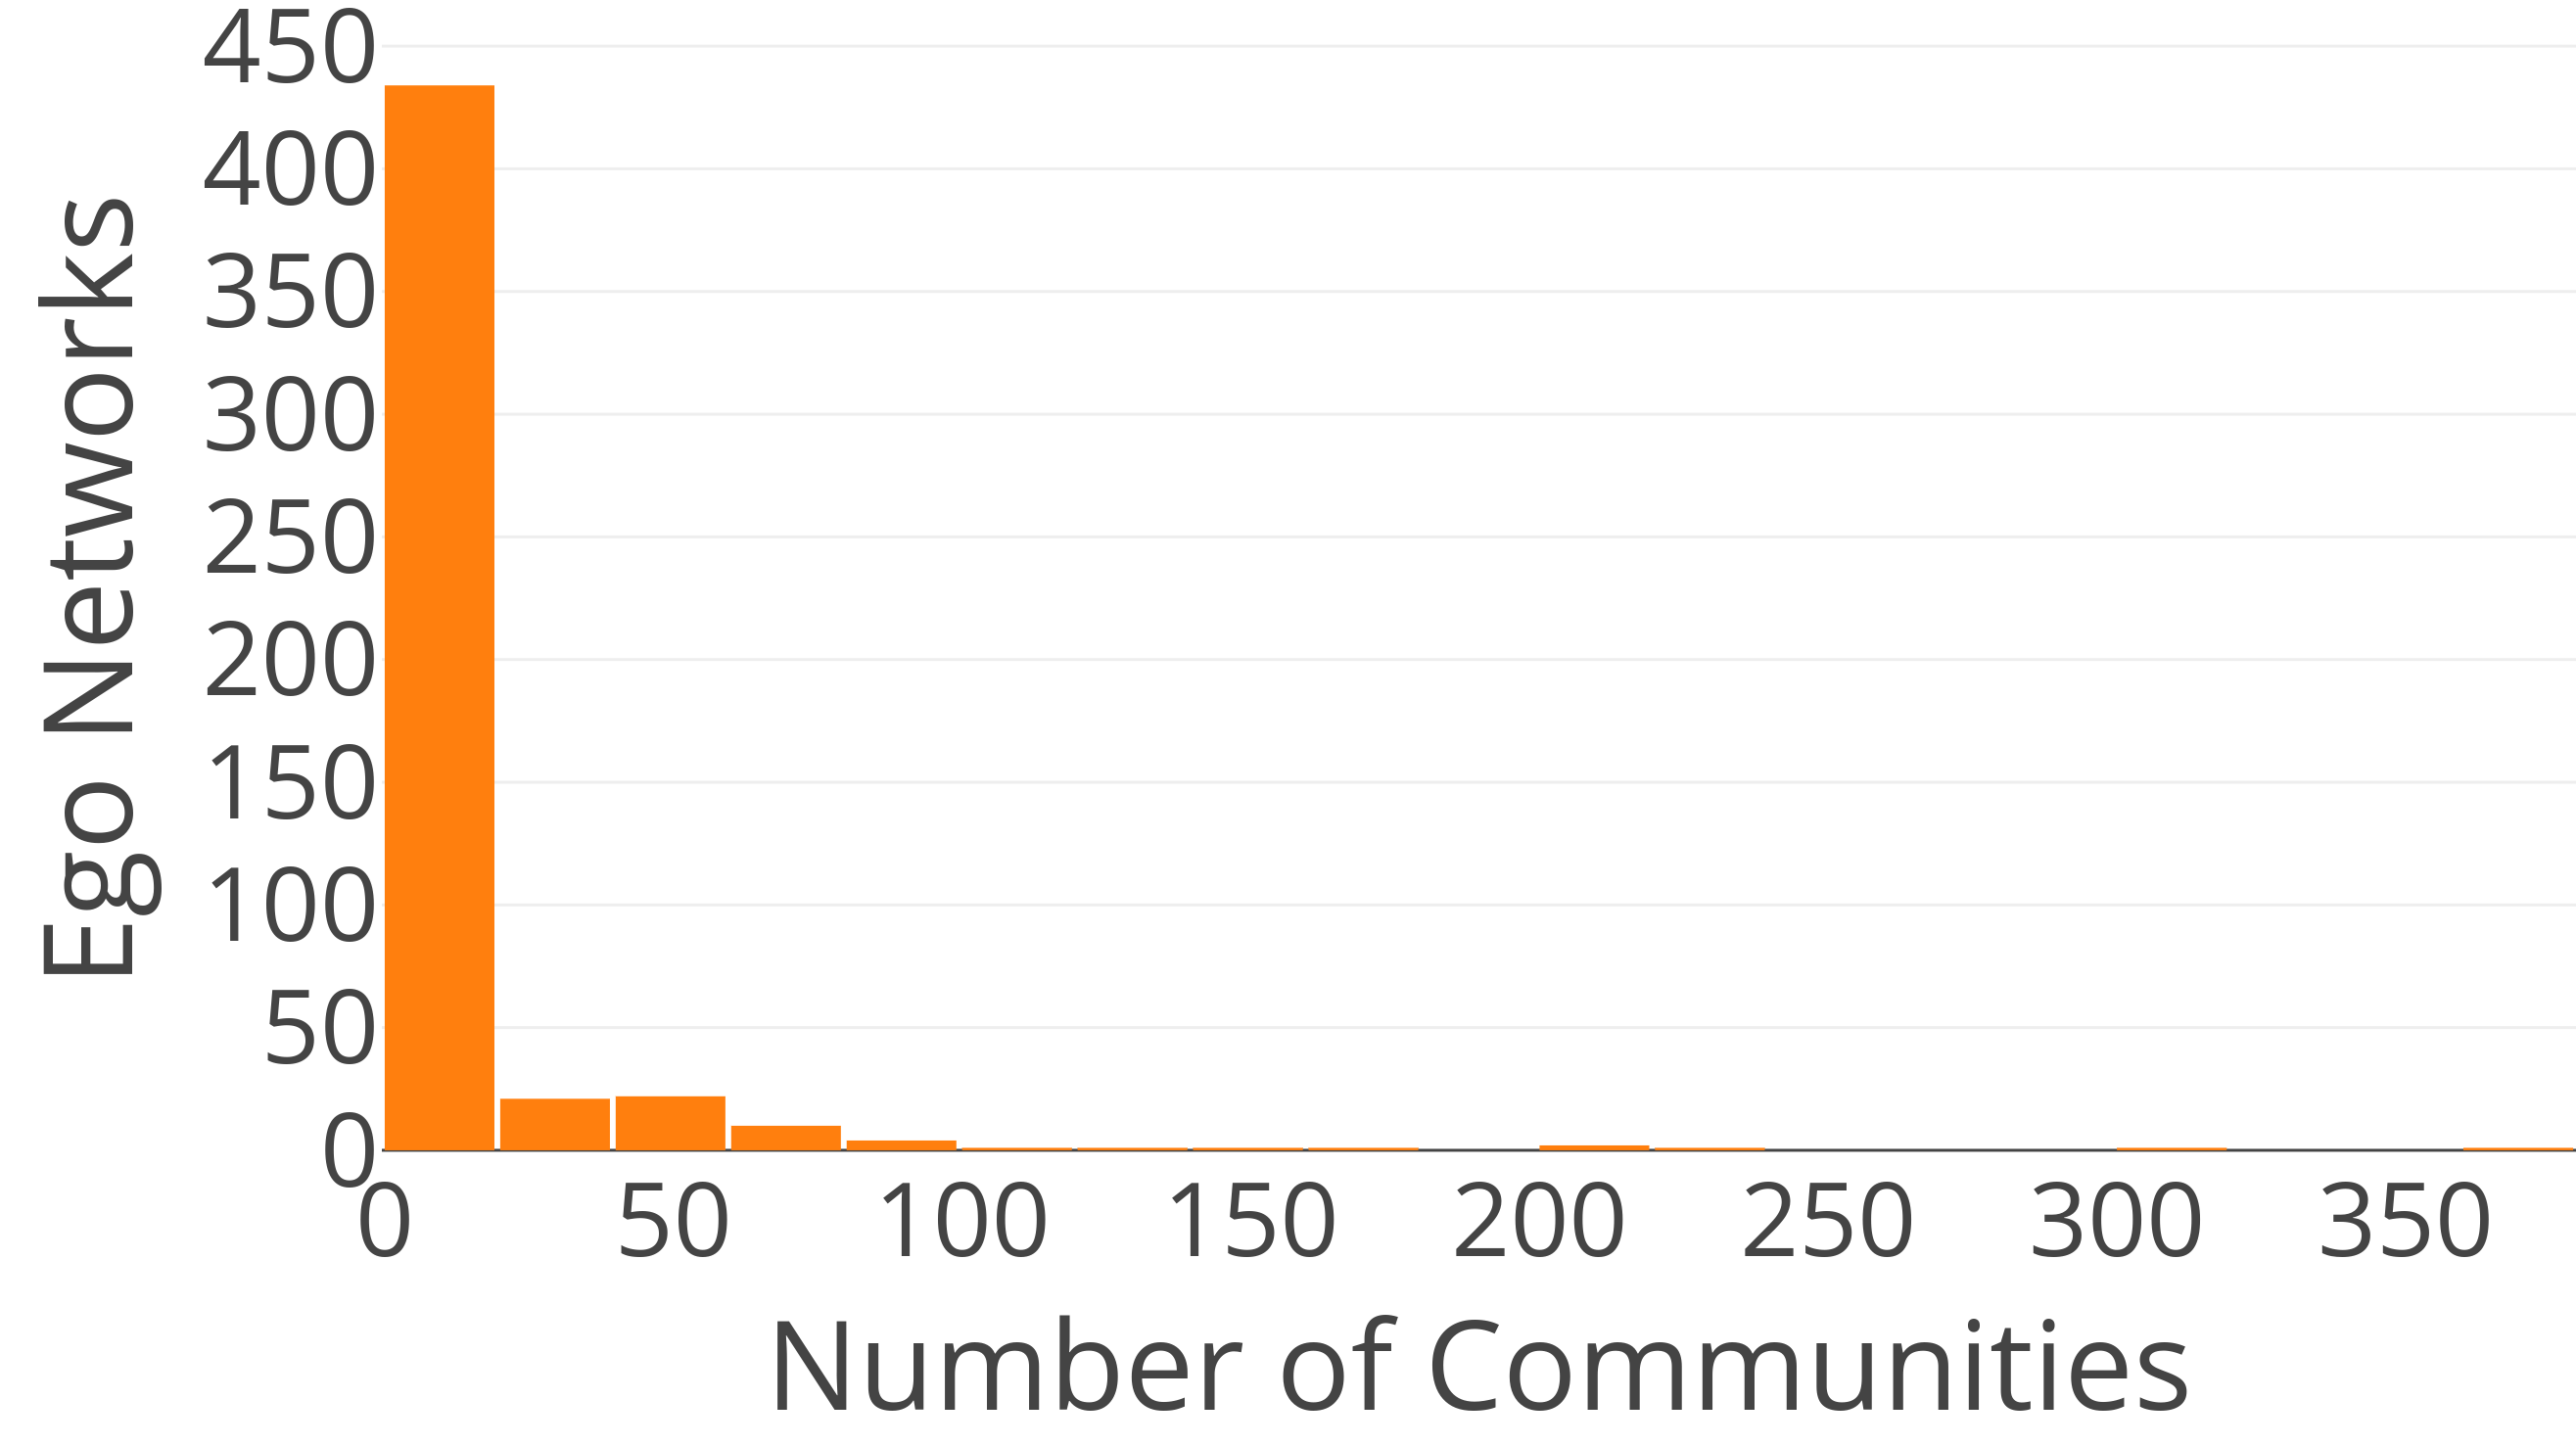
\includegraphics[width=0.47\textwidth]{fig/comm_stats/rak/n_comm/n_comm_rak_retweet.png}
        \label{fig:comm_stats_n_comm_rak_retweet}
    } \\
    \subfigure[Like]{
        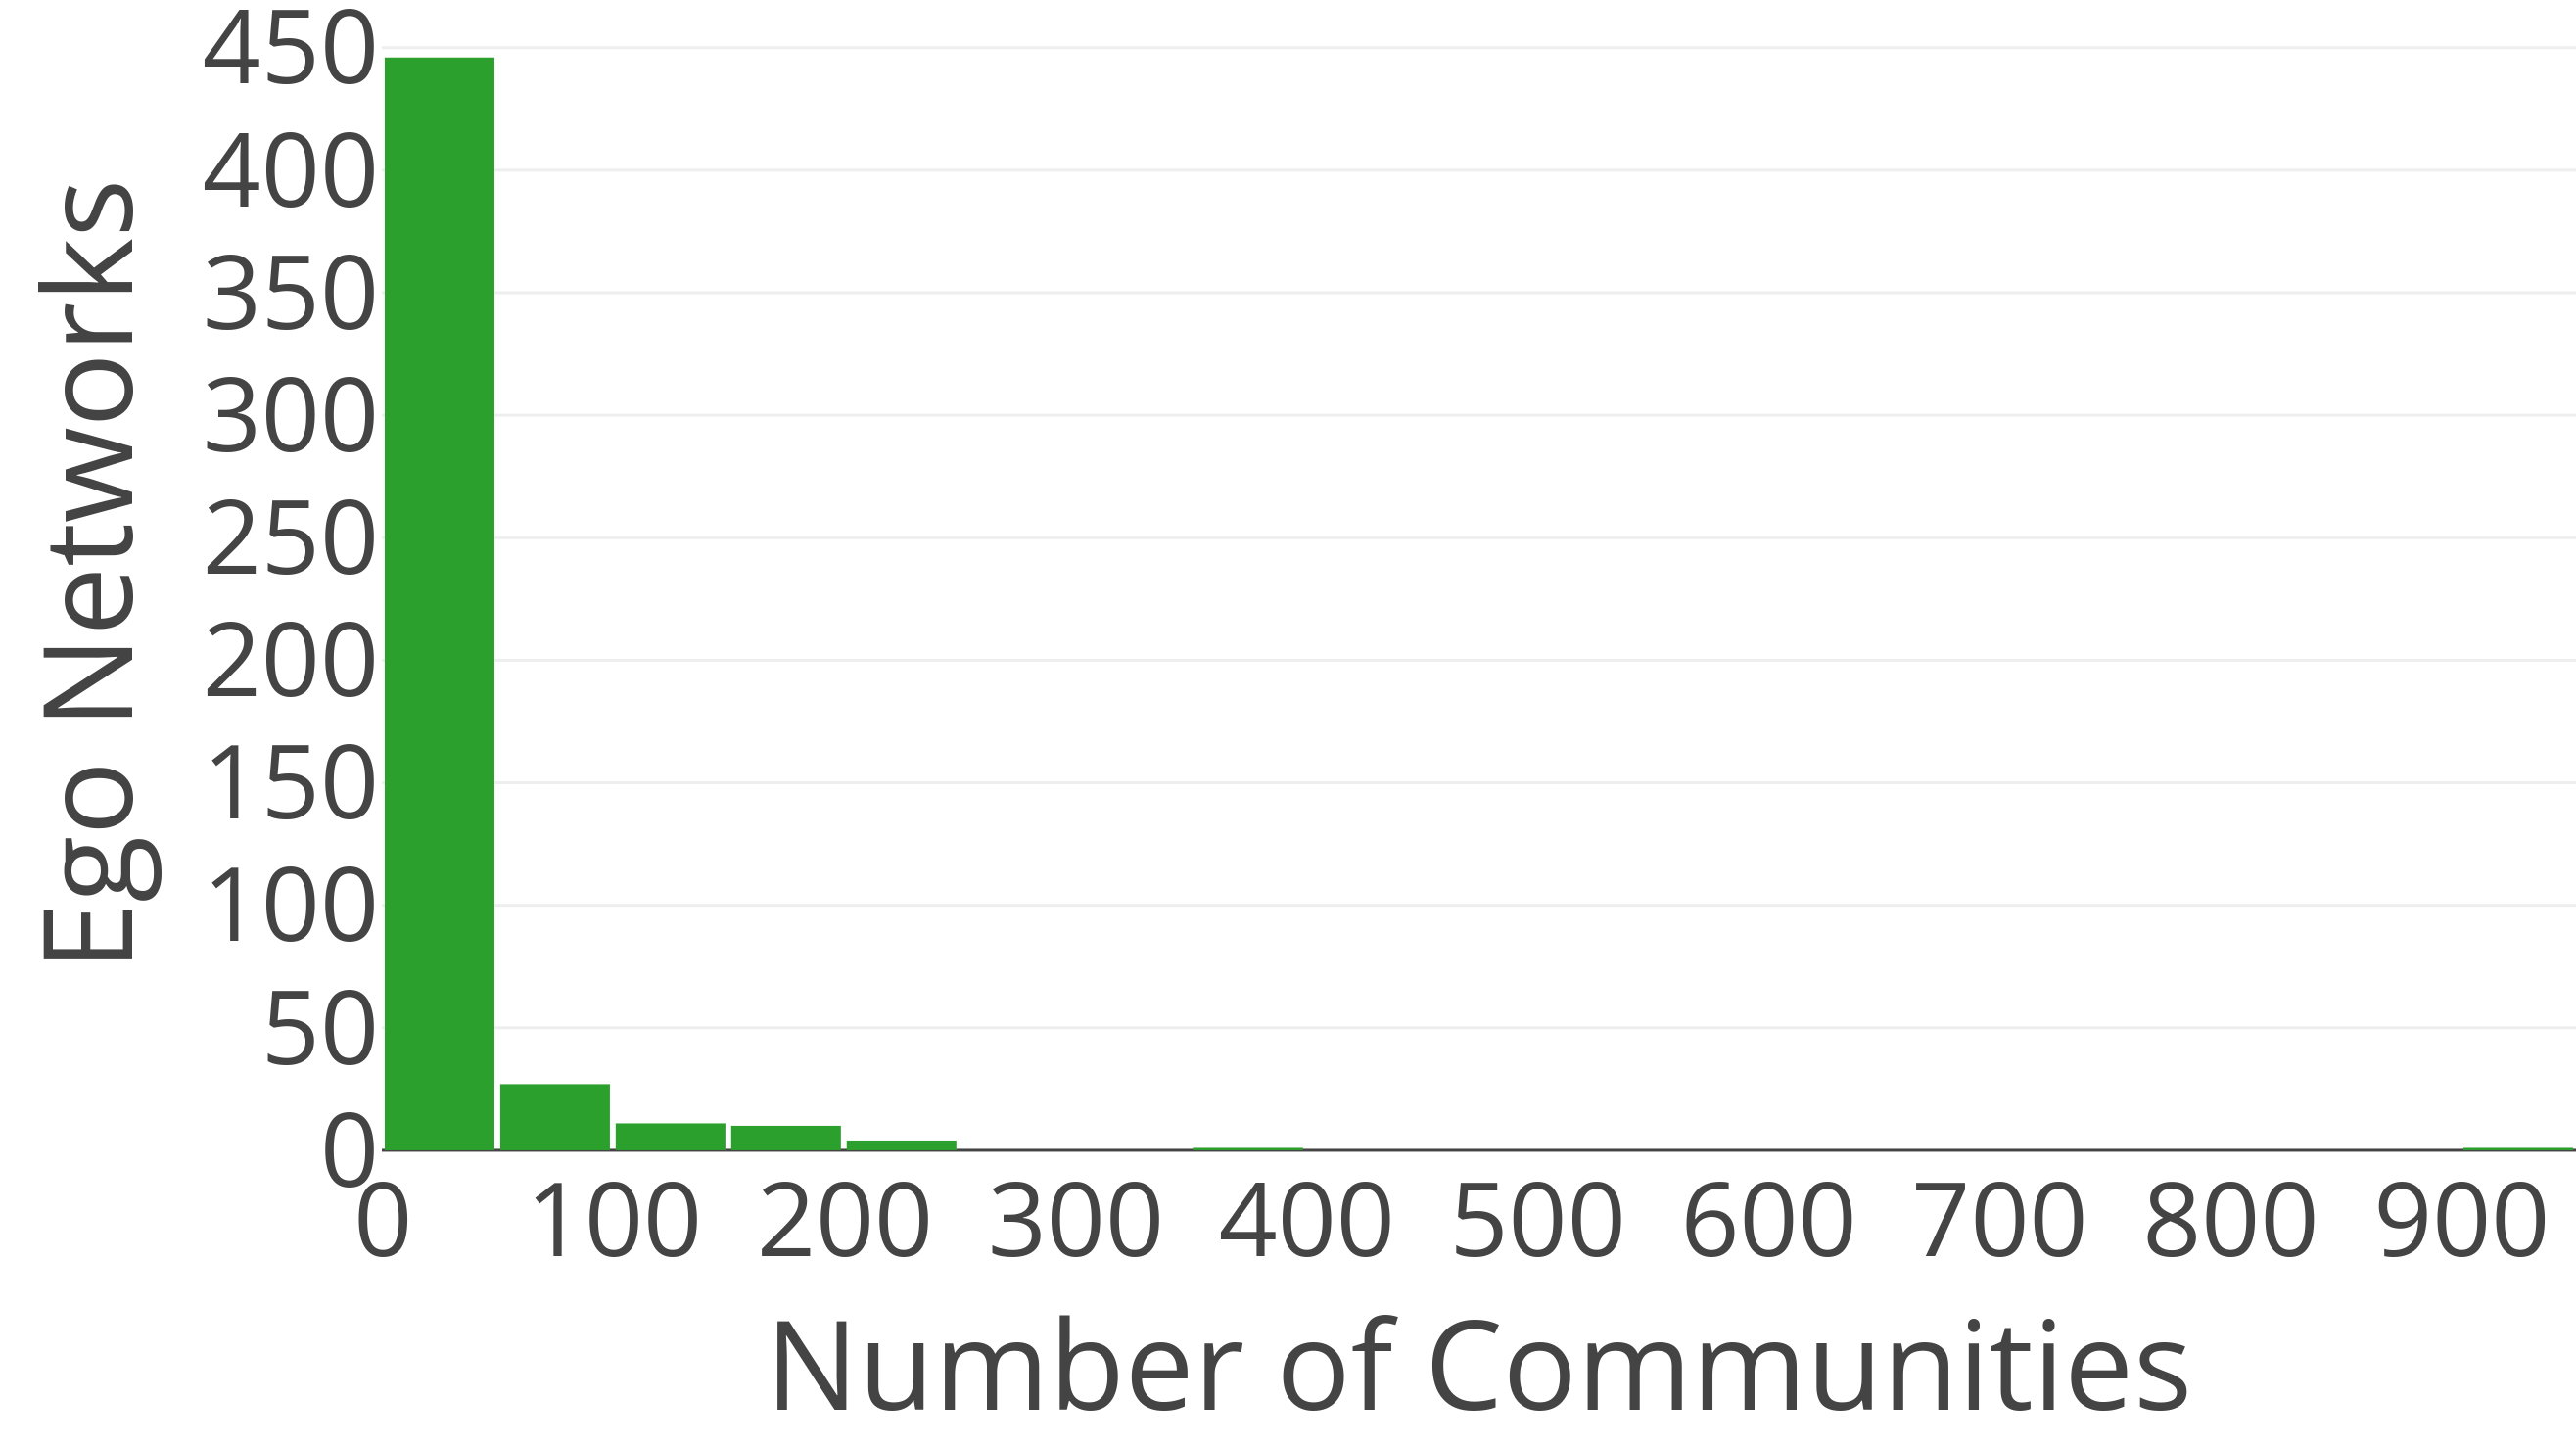
\includegraphics[width=0.47\textwidth]{fig/comm_stats/rak/n_comm/n_comm_rak_like.png}
        \label{fig:comm_stats_n_comm_rak_like}
    }
    \subfigure[Mention]{
        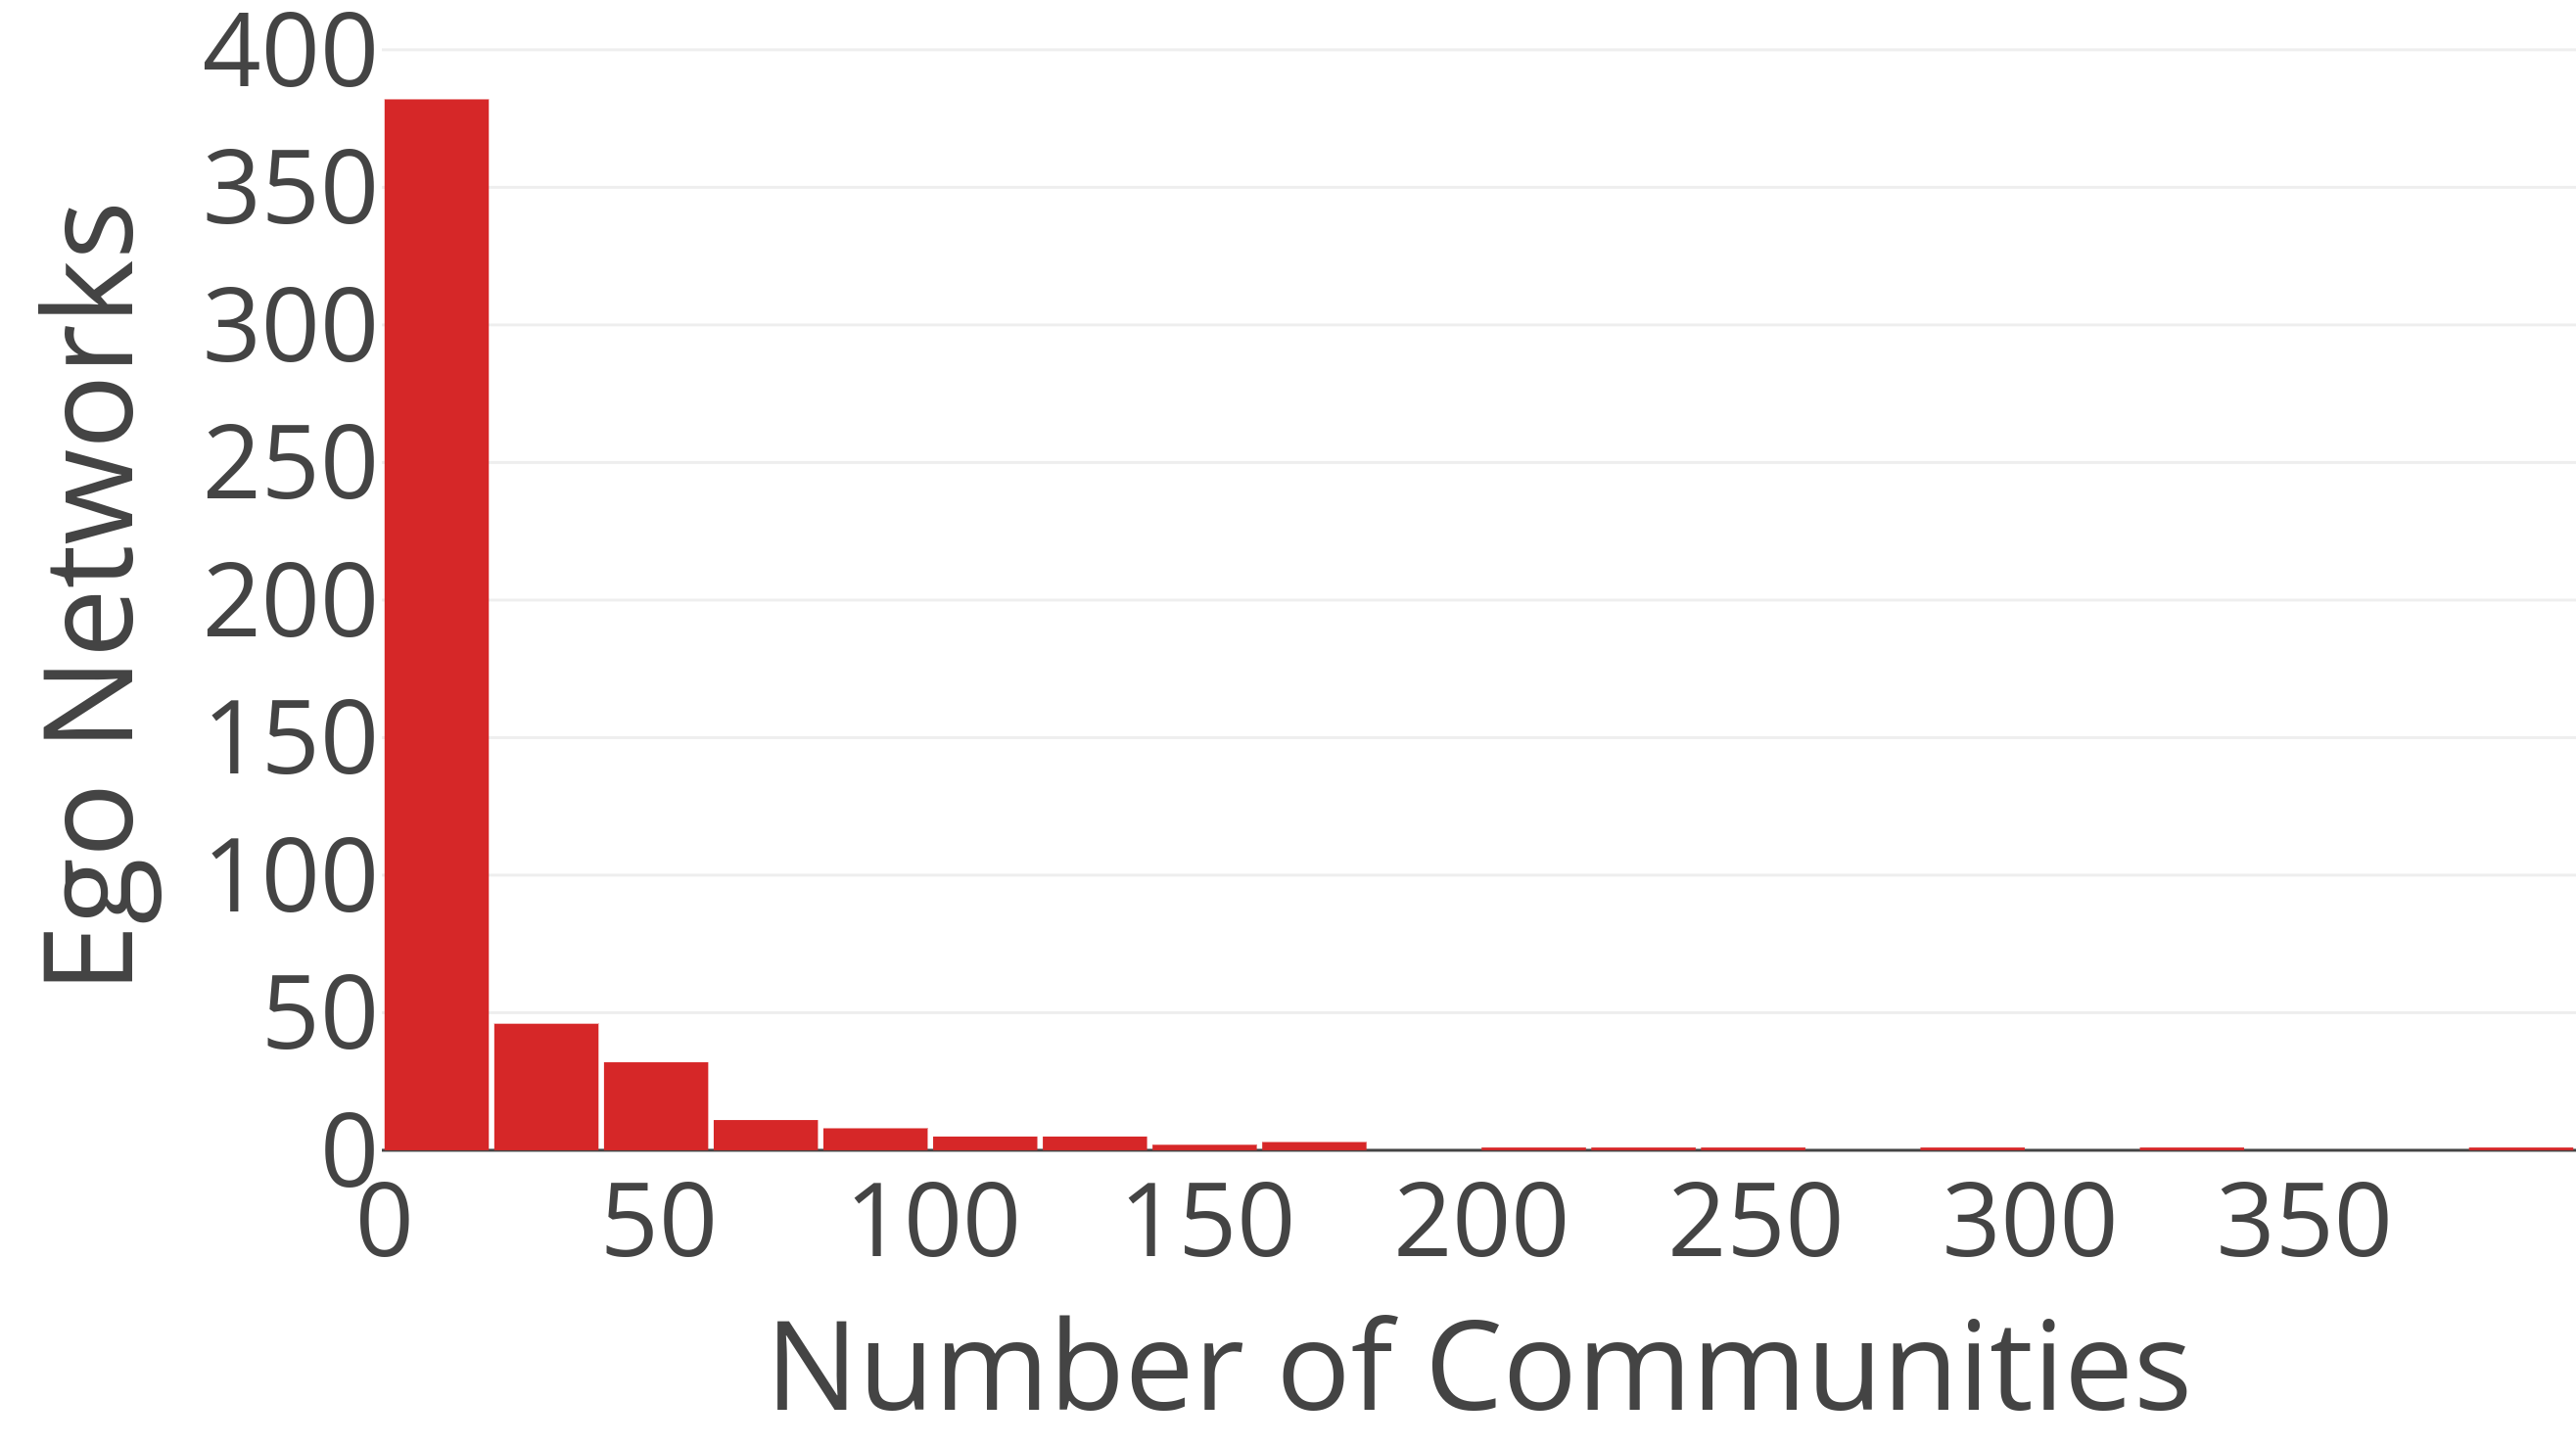
\includegraphics[width=0.47\textwidth]{fig/comm_stats/rak/n_comm/n_comm_rak_mention.png}
        \label{fig:comm_stats_n_comm_rak_mention}
    }
    \caption{Number of communities detected by RAK.}
    \label{fig:comm_stats_n_comm_rak}
    
\end{figure}

\begin{figure}[h!tb]
    \centering
    \subfigure[Follow]{
        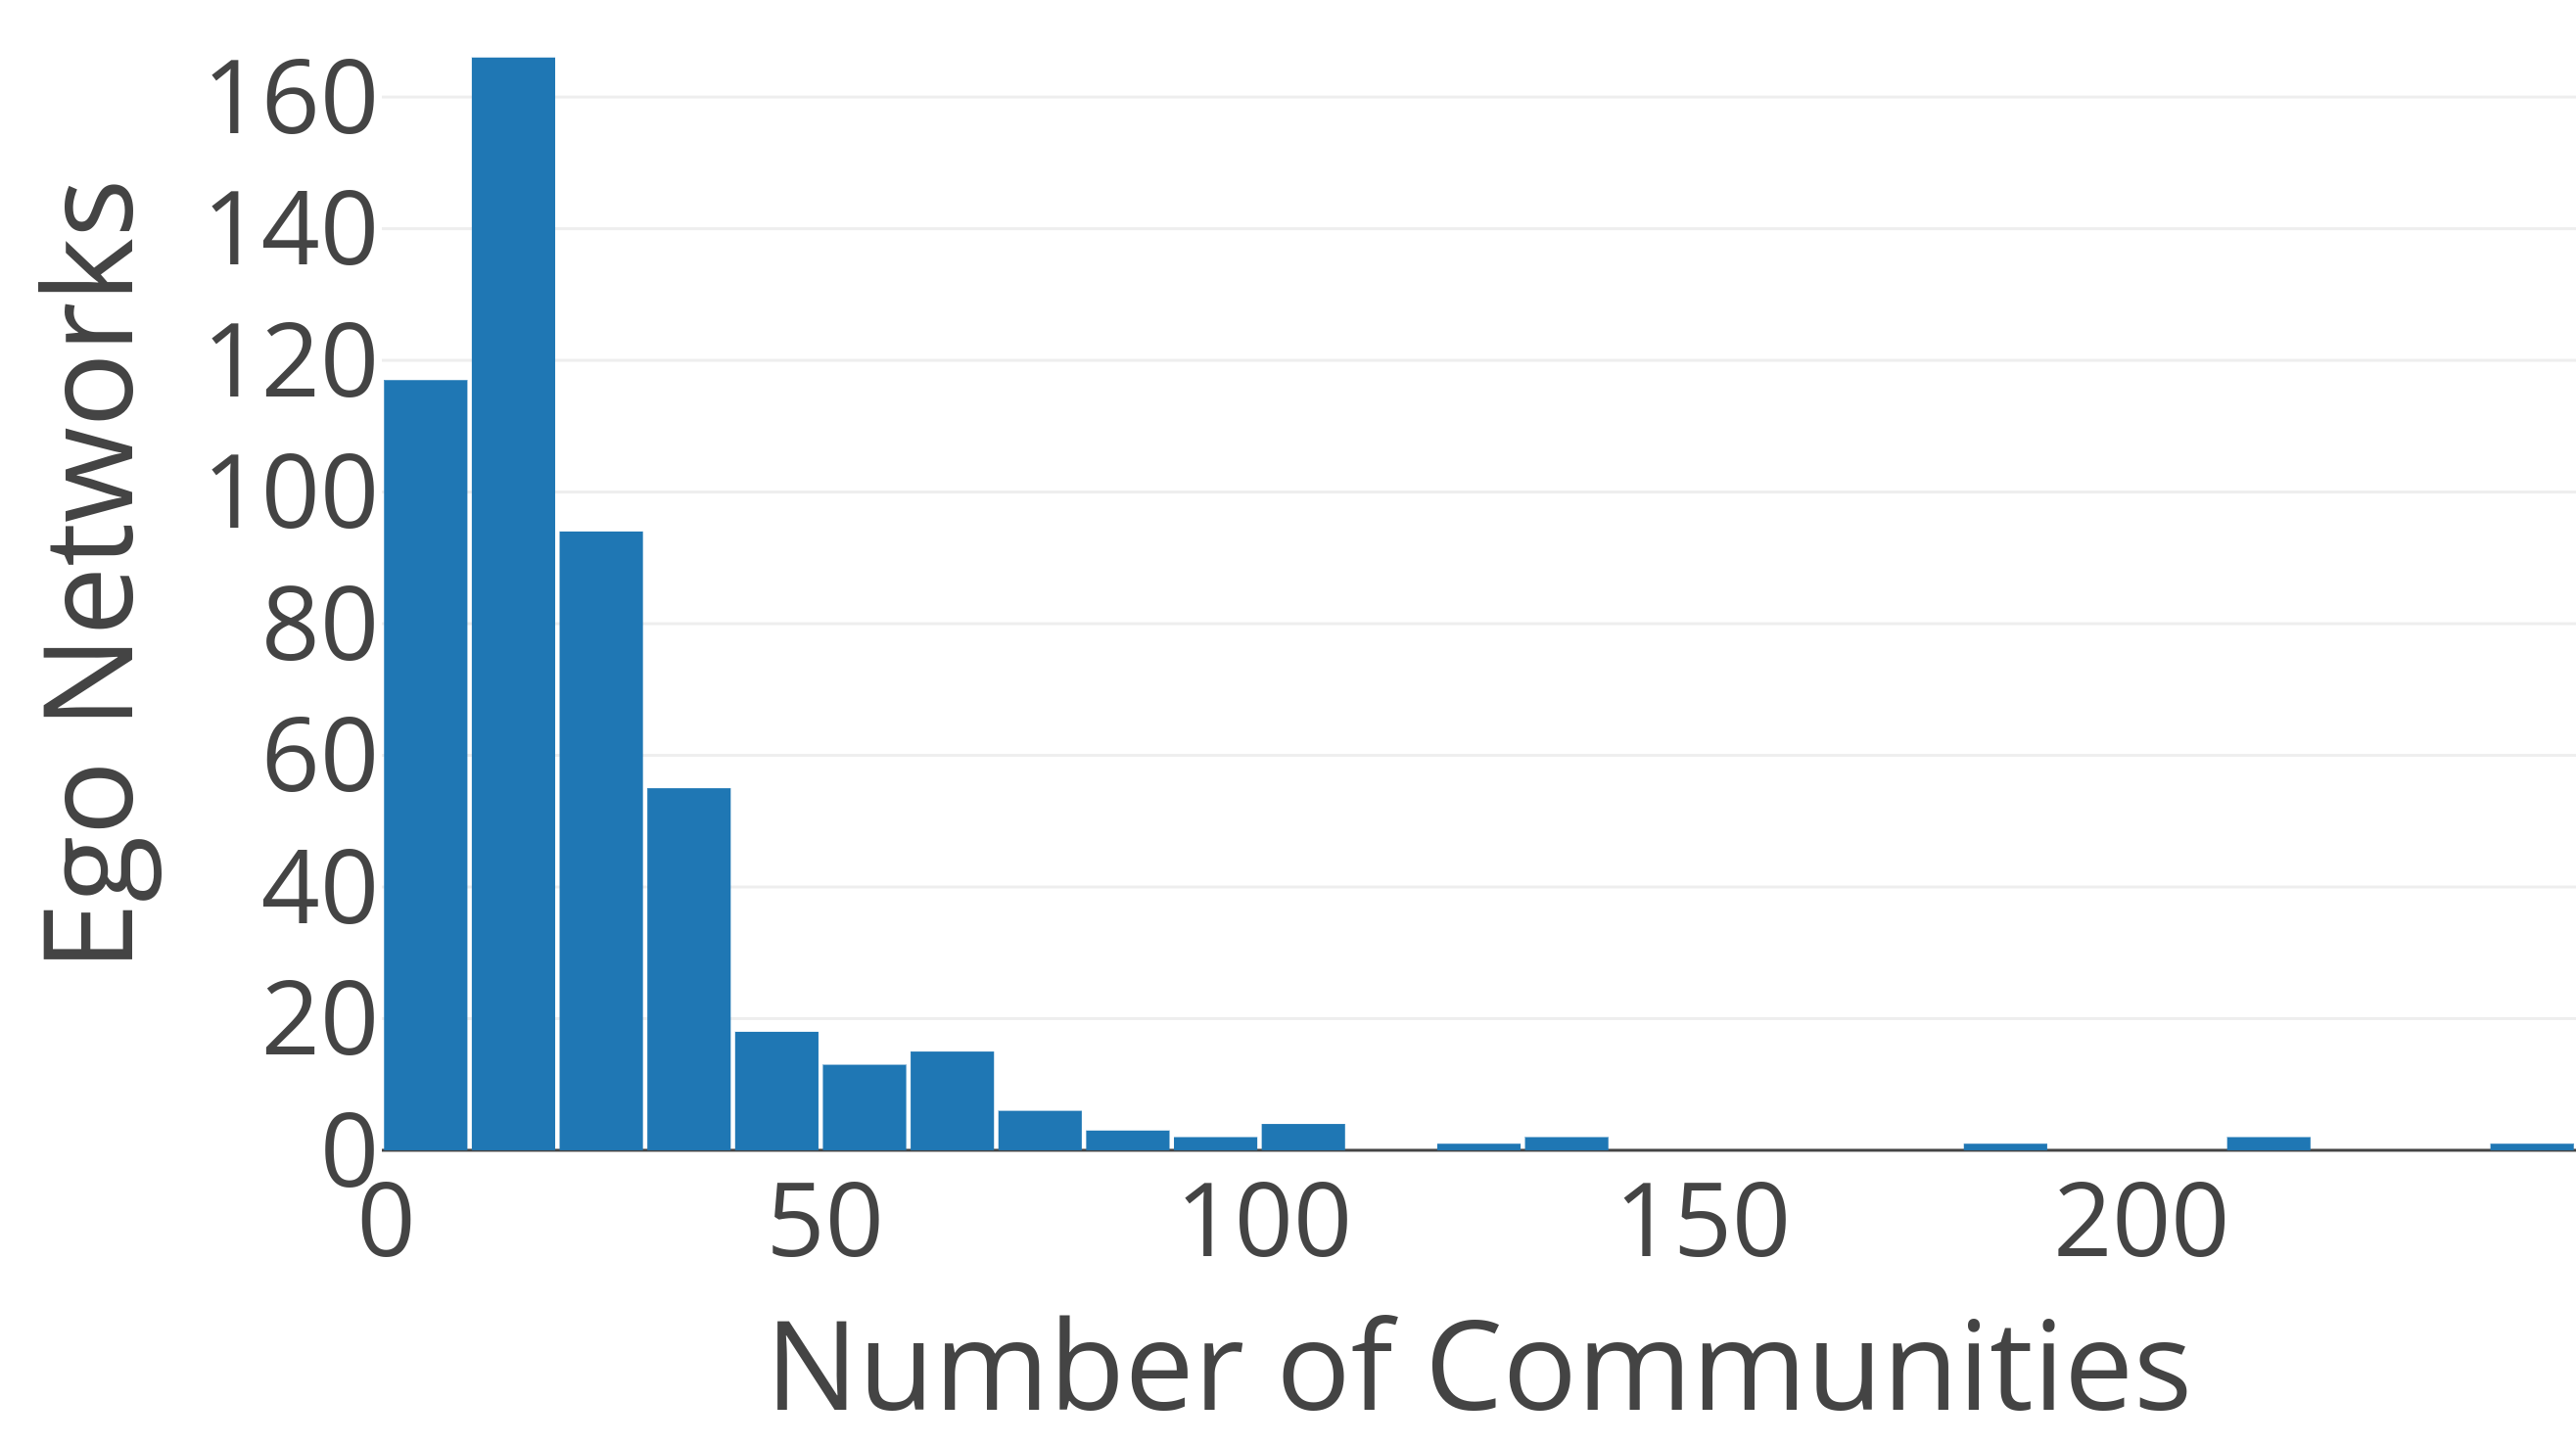
\includegraphics[width=0.47\textwidth]{fig/comm_stats/infomap/n_comm/n_comm_infomap_follow.png}
        \label{fig:comm_stats_n_comm_infomap_follow}
    }
    \subfigure[Retweet]{
        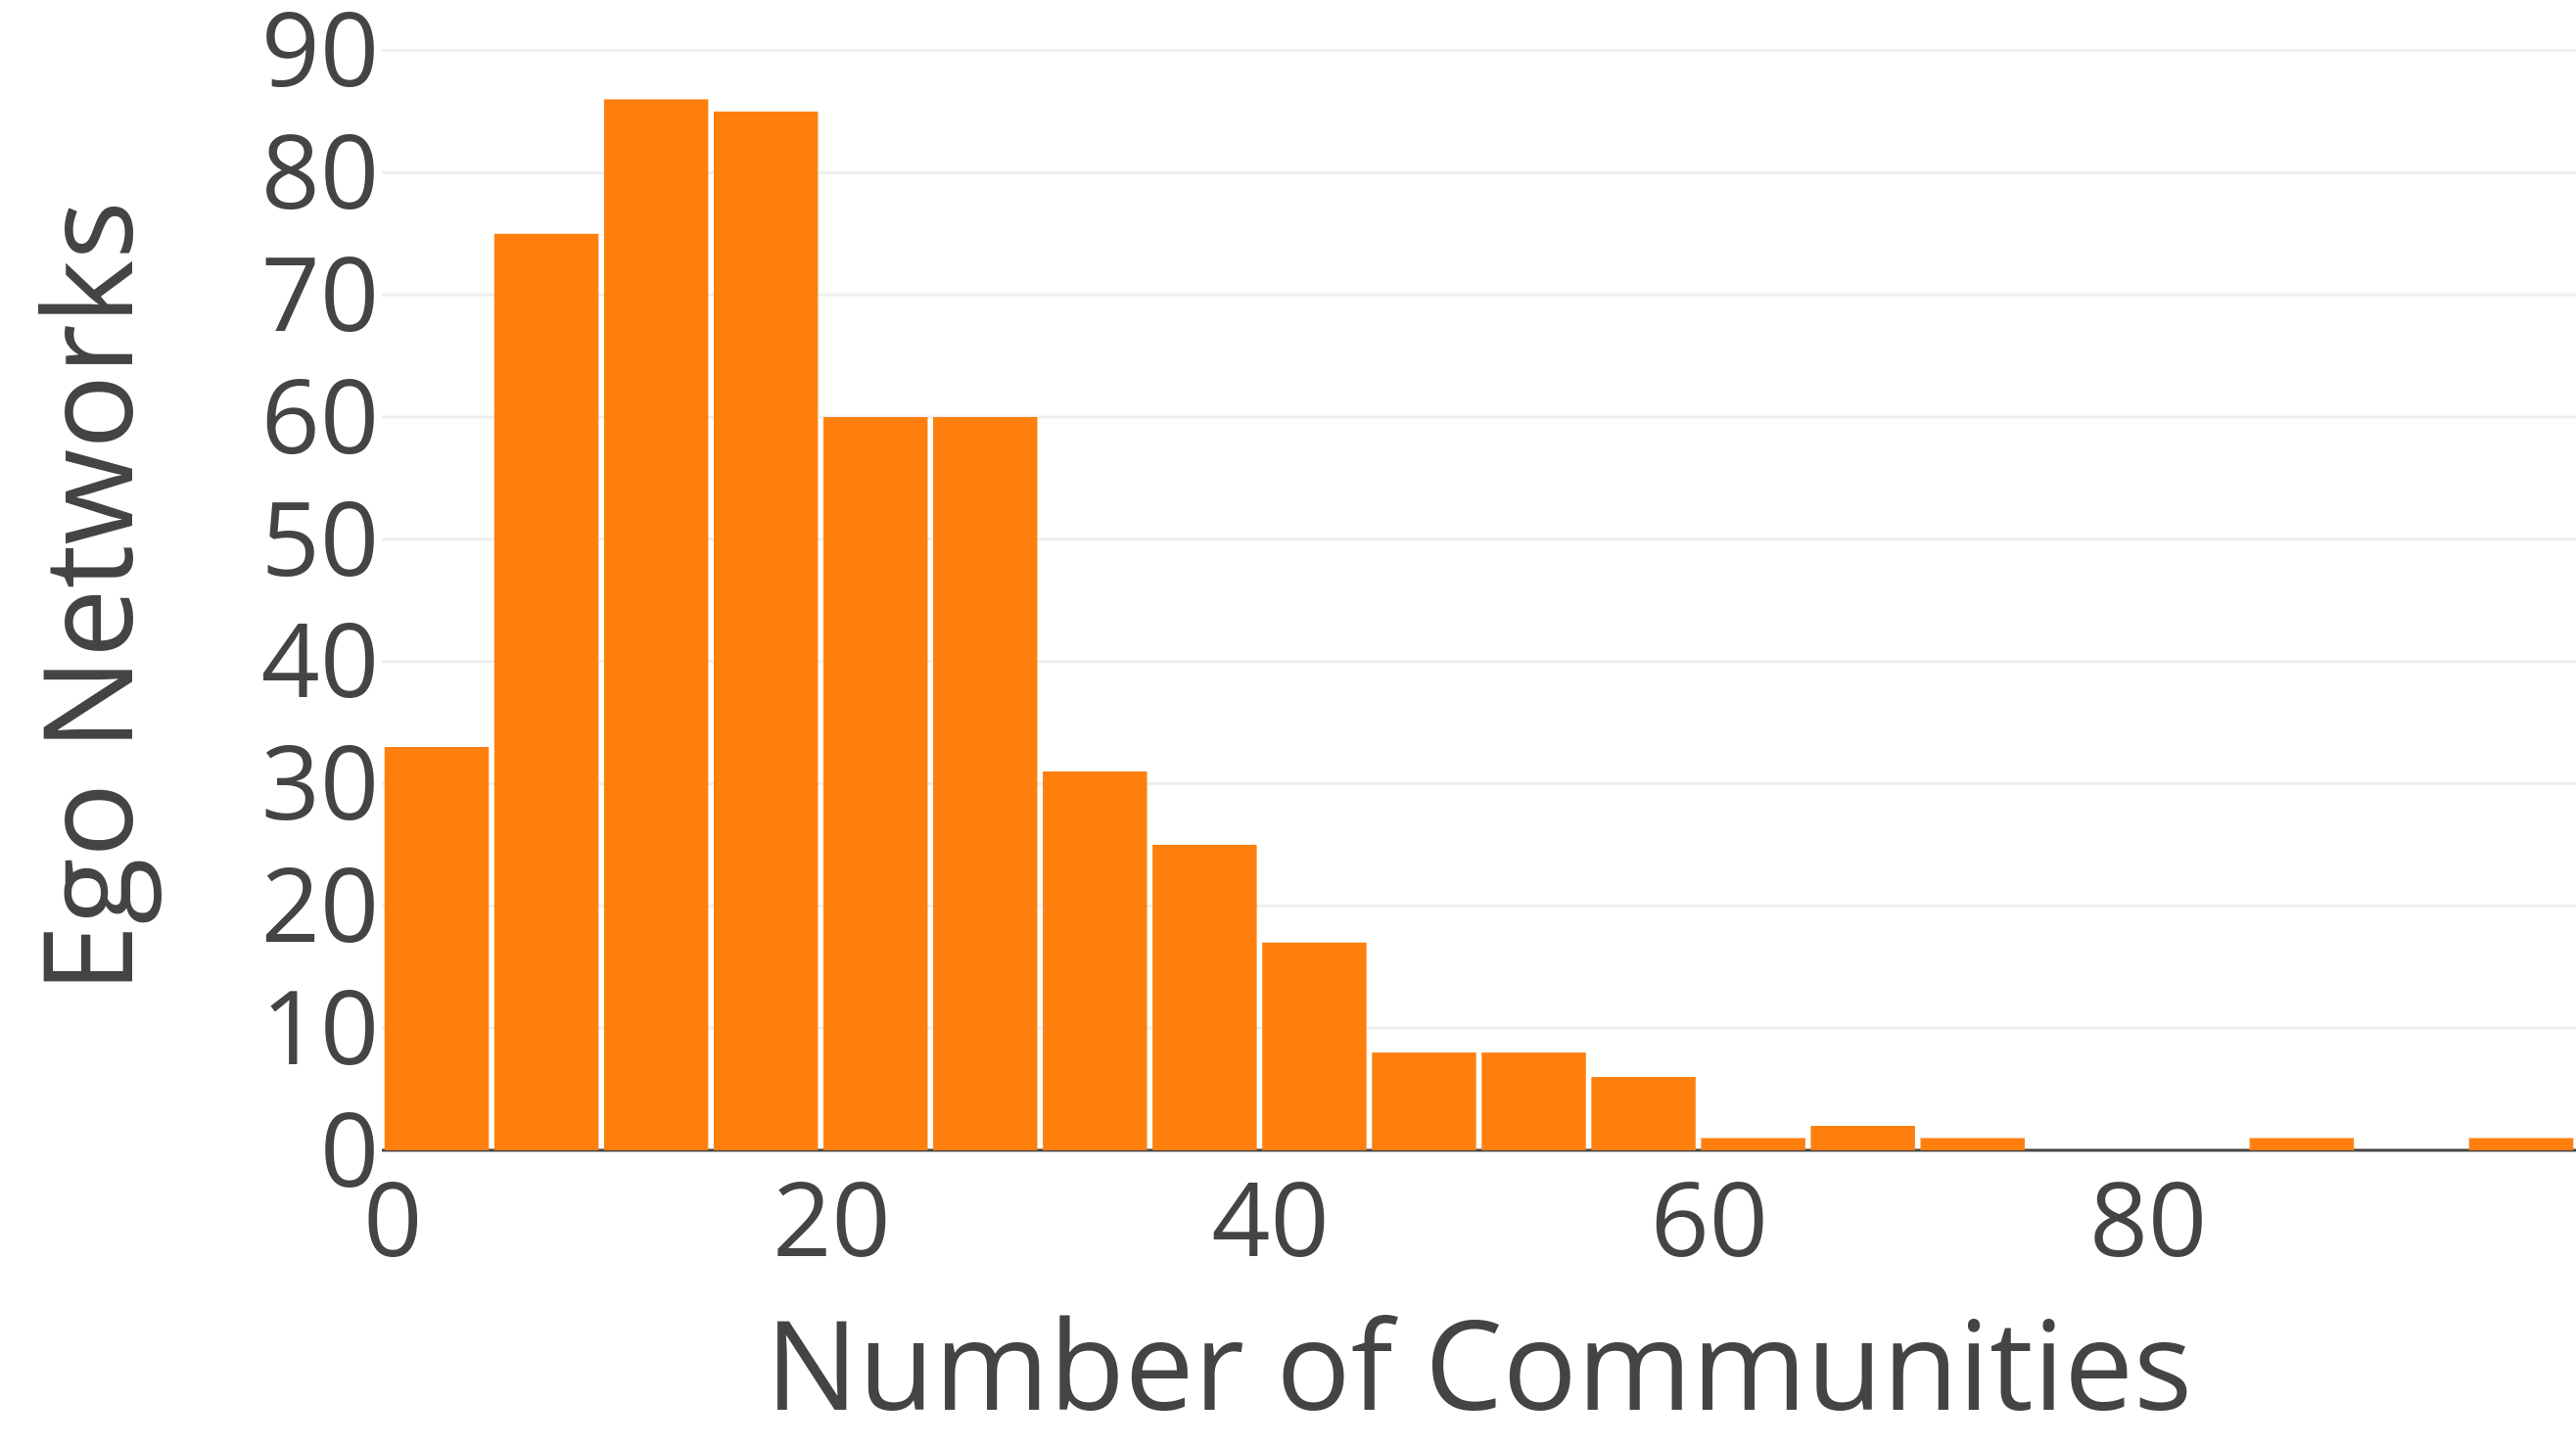
\includegraphics[width=0.47\textwidth]{fig/comm_stats/infomap/n_comm/n_comm_infomap_retweet.png}
        \label{fig:comm_stats_n_comm_infomap_retweet}
    } \\
    \subfigure[Like]{
        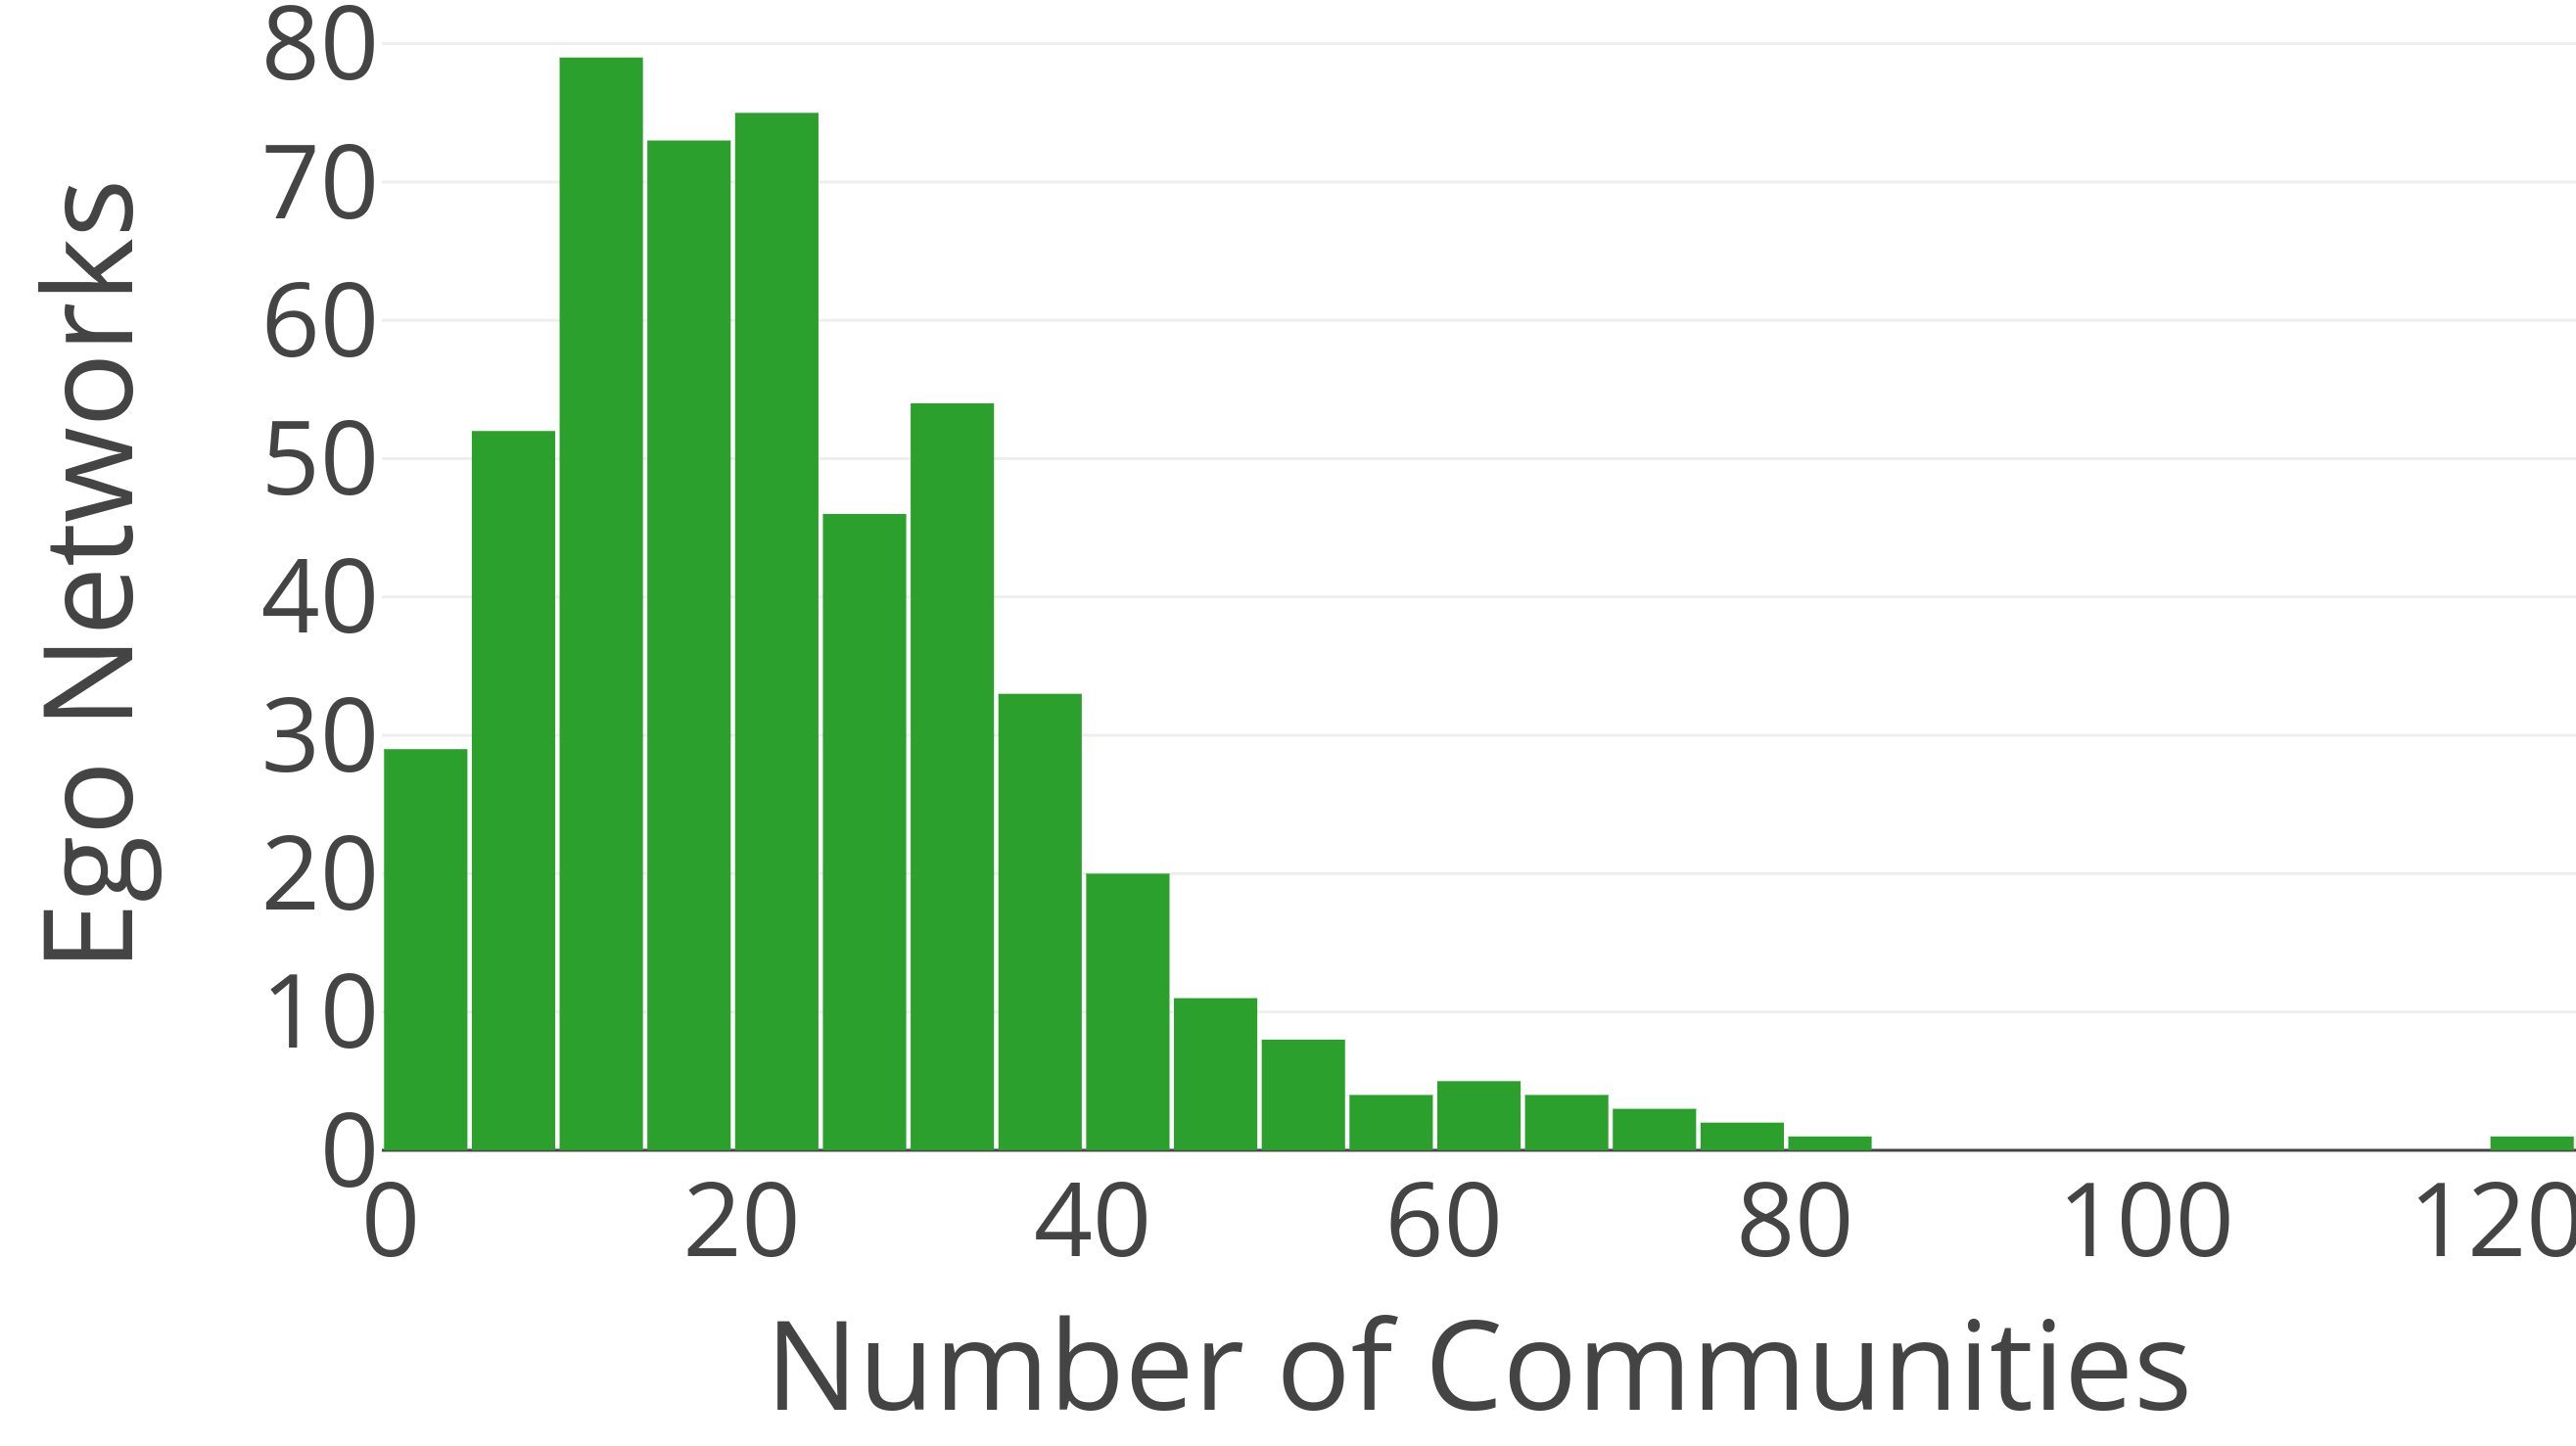
\includegraphics[width=0.47\textwidth]{fig/comm_stats/infomap/n_comm/n_comm_infomap_like.png}
        \label{fig:comm_stats_n_comm_infomap_like}
    }
    \subfigure[Mention]{
        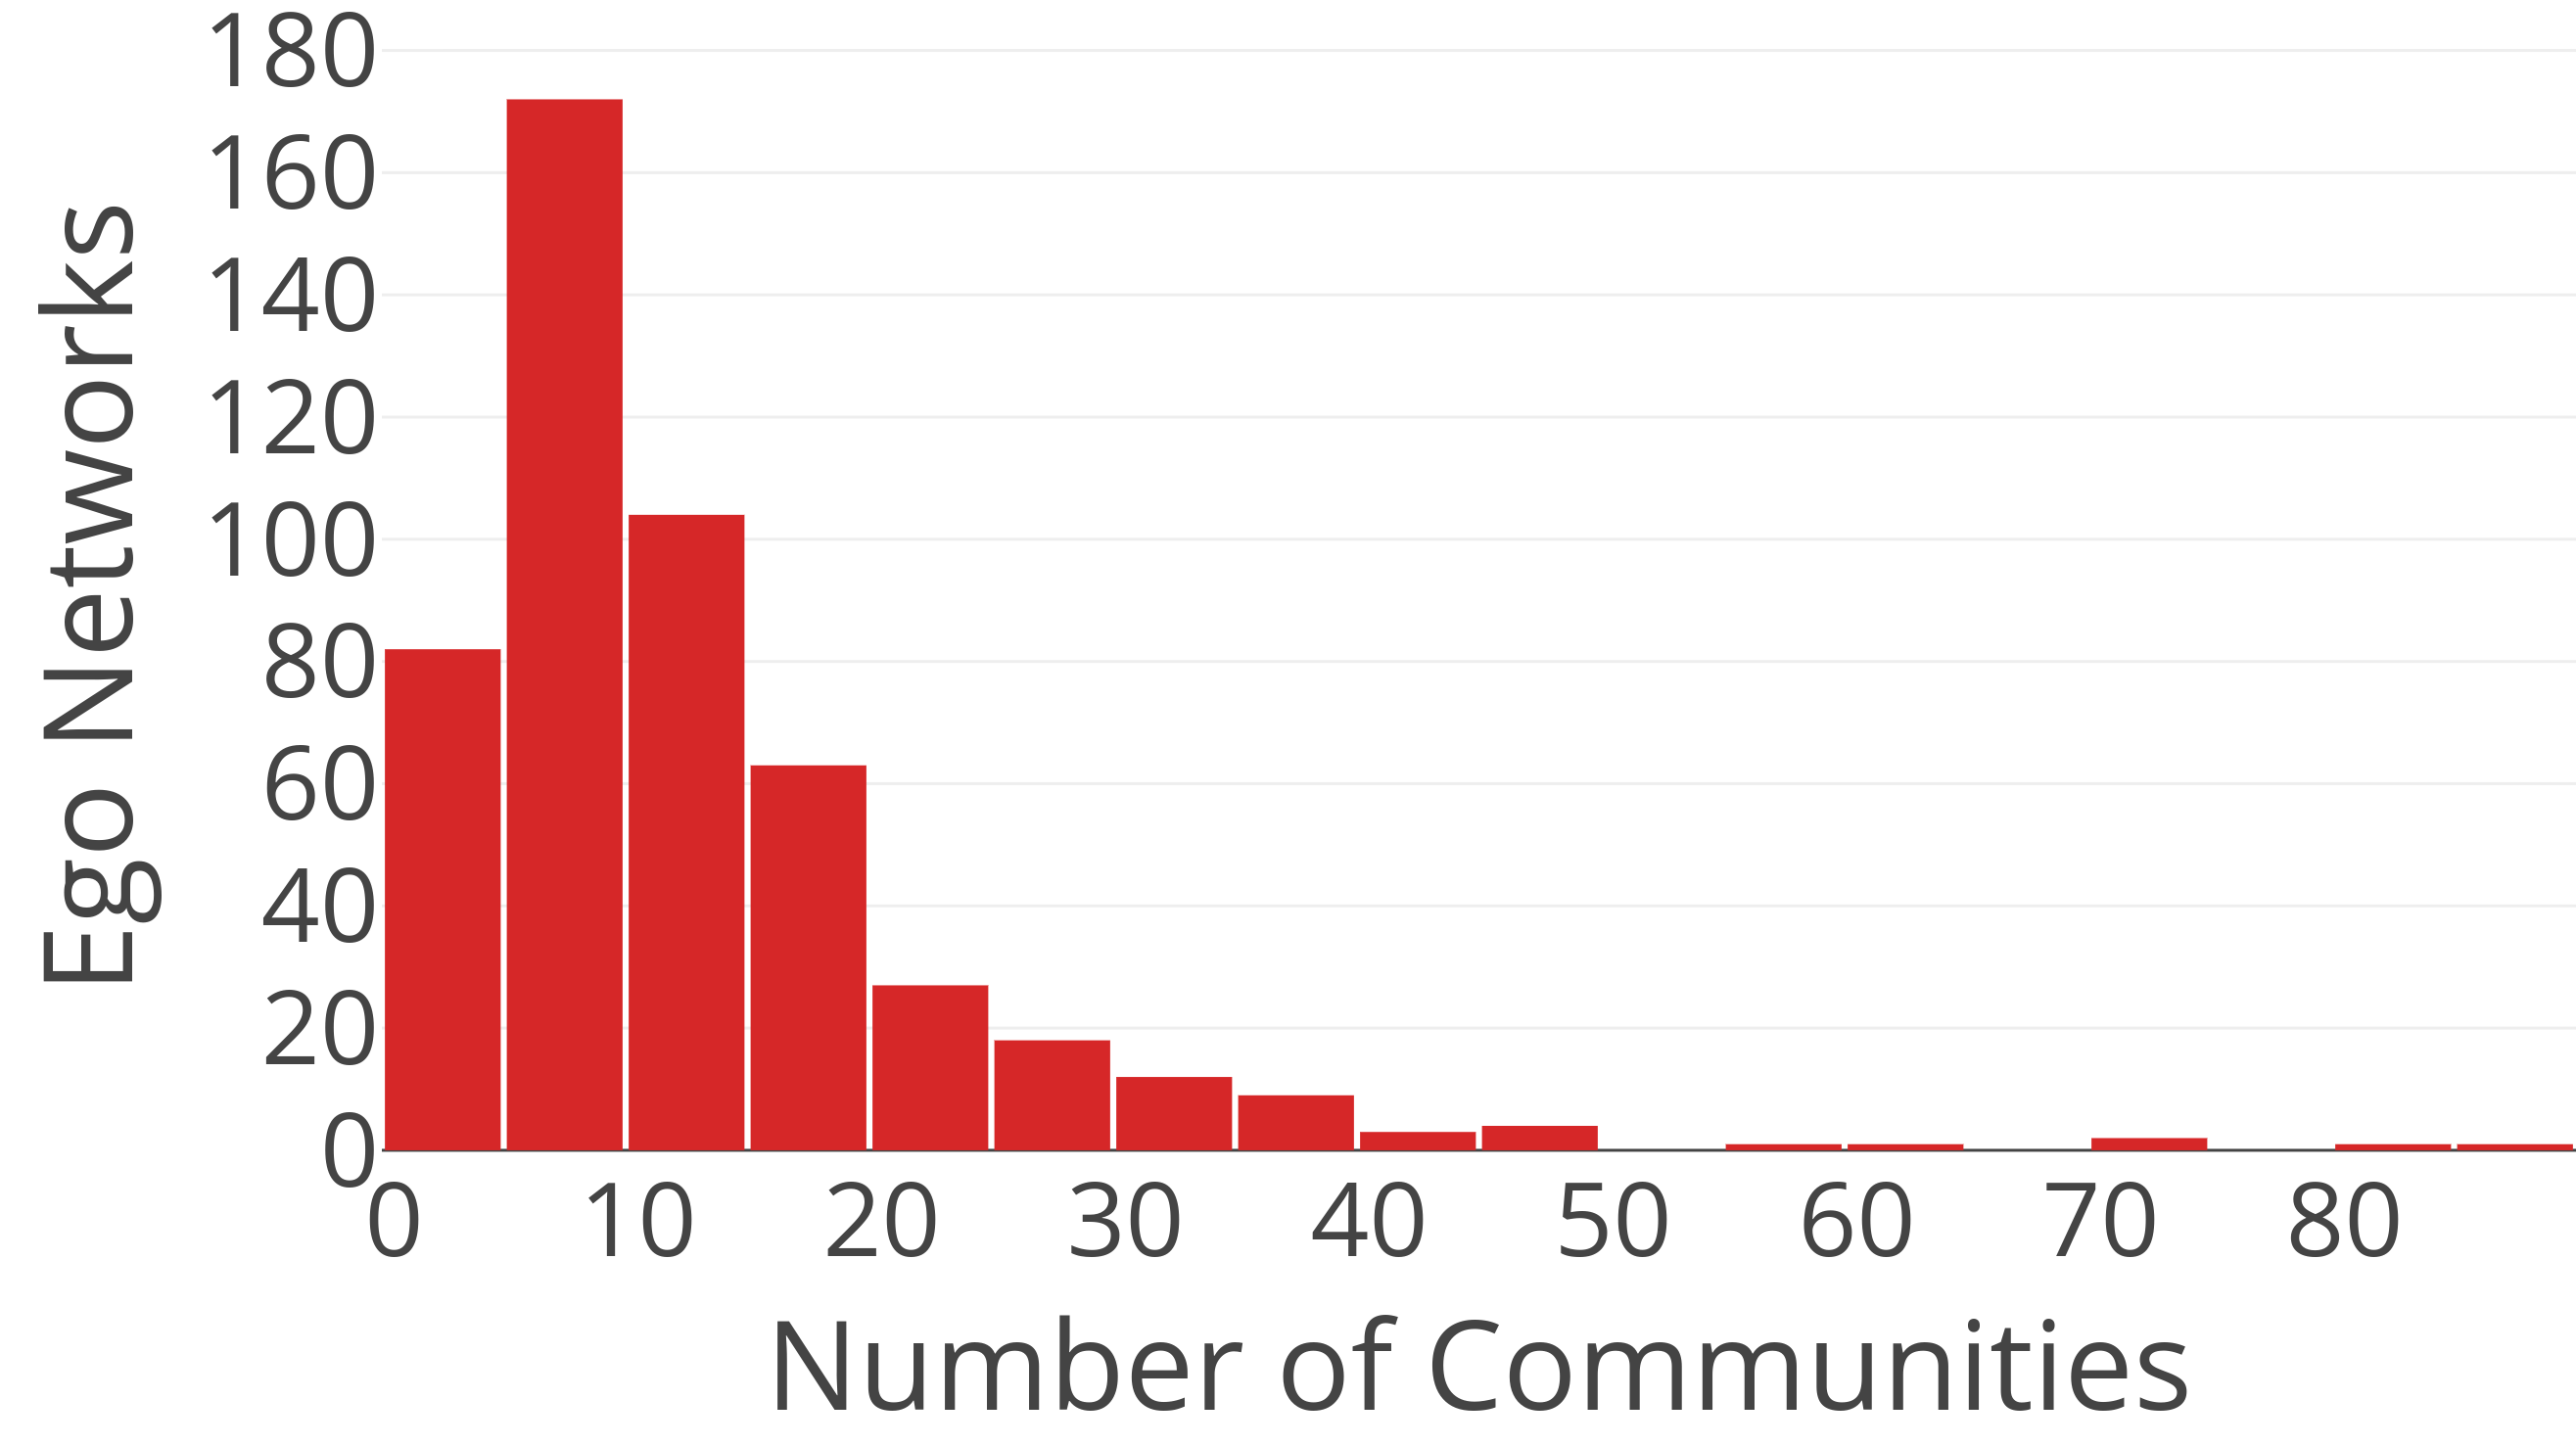
\includegraphics[width=0.47\textwidth]{fig/comm_stats/infomap/n_comm/n_comm_infomap_mention.png}
        \label{fig:comm_stats_n_comm_infomap_mention}
    }
    \caption{Number of communities detected by INFOMAP.}
    \label{fig:comm_stats_n_comm_infomap}
\end{figure}
\begin{figure}[h!tb]
    \centering
    \subfigure[Follow]{
        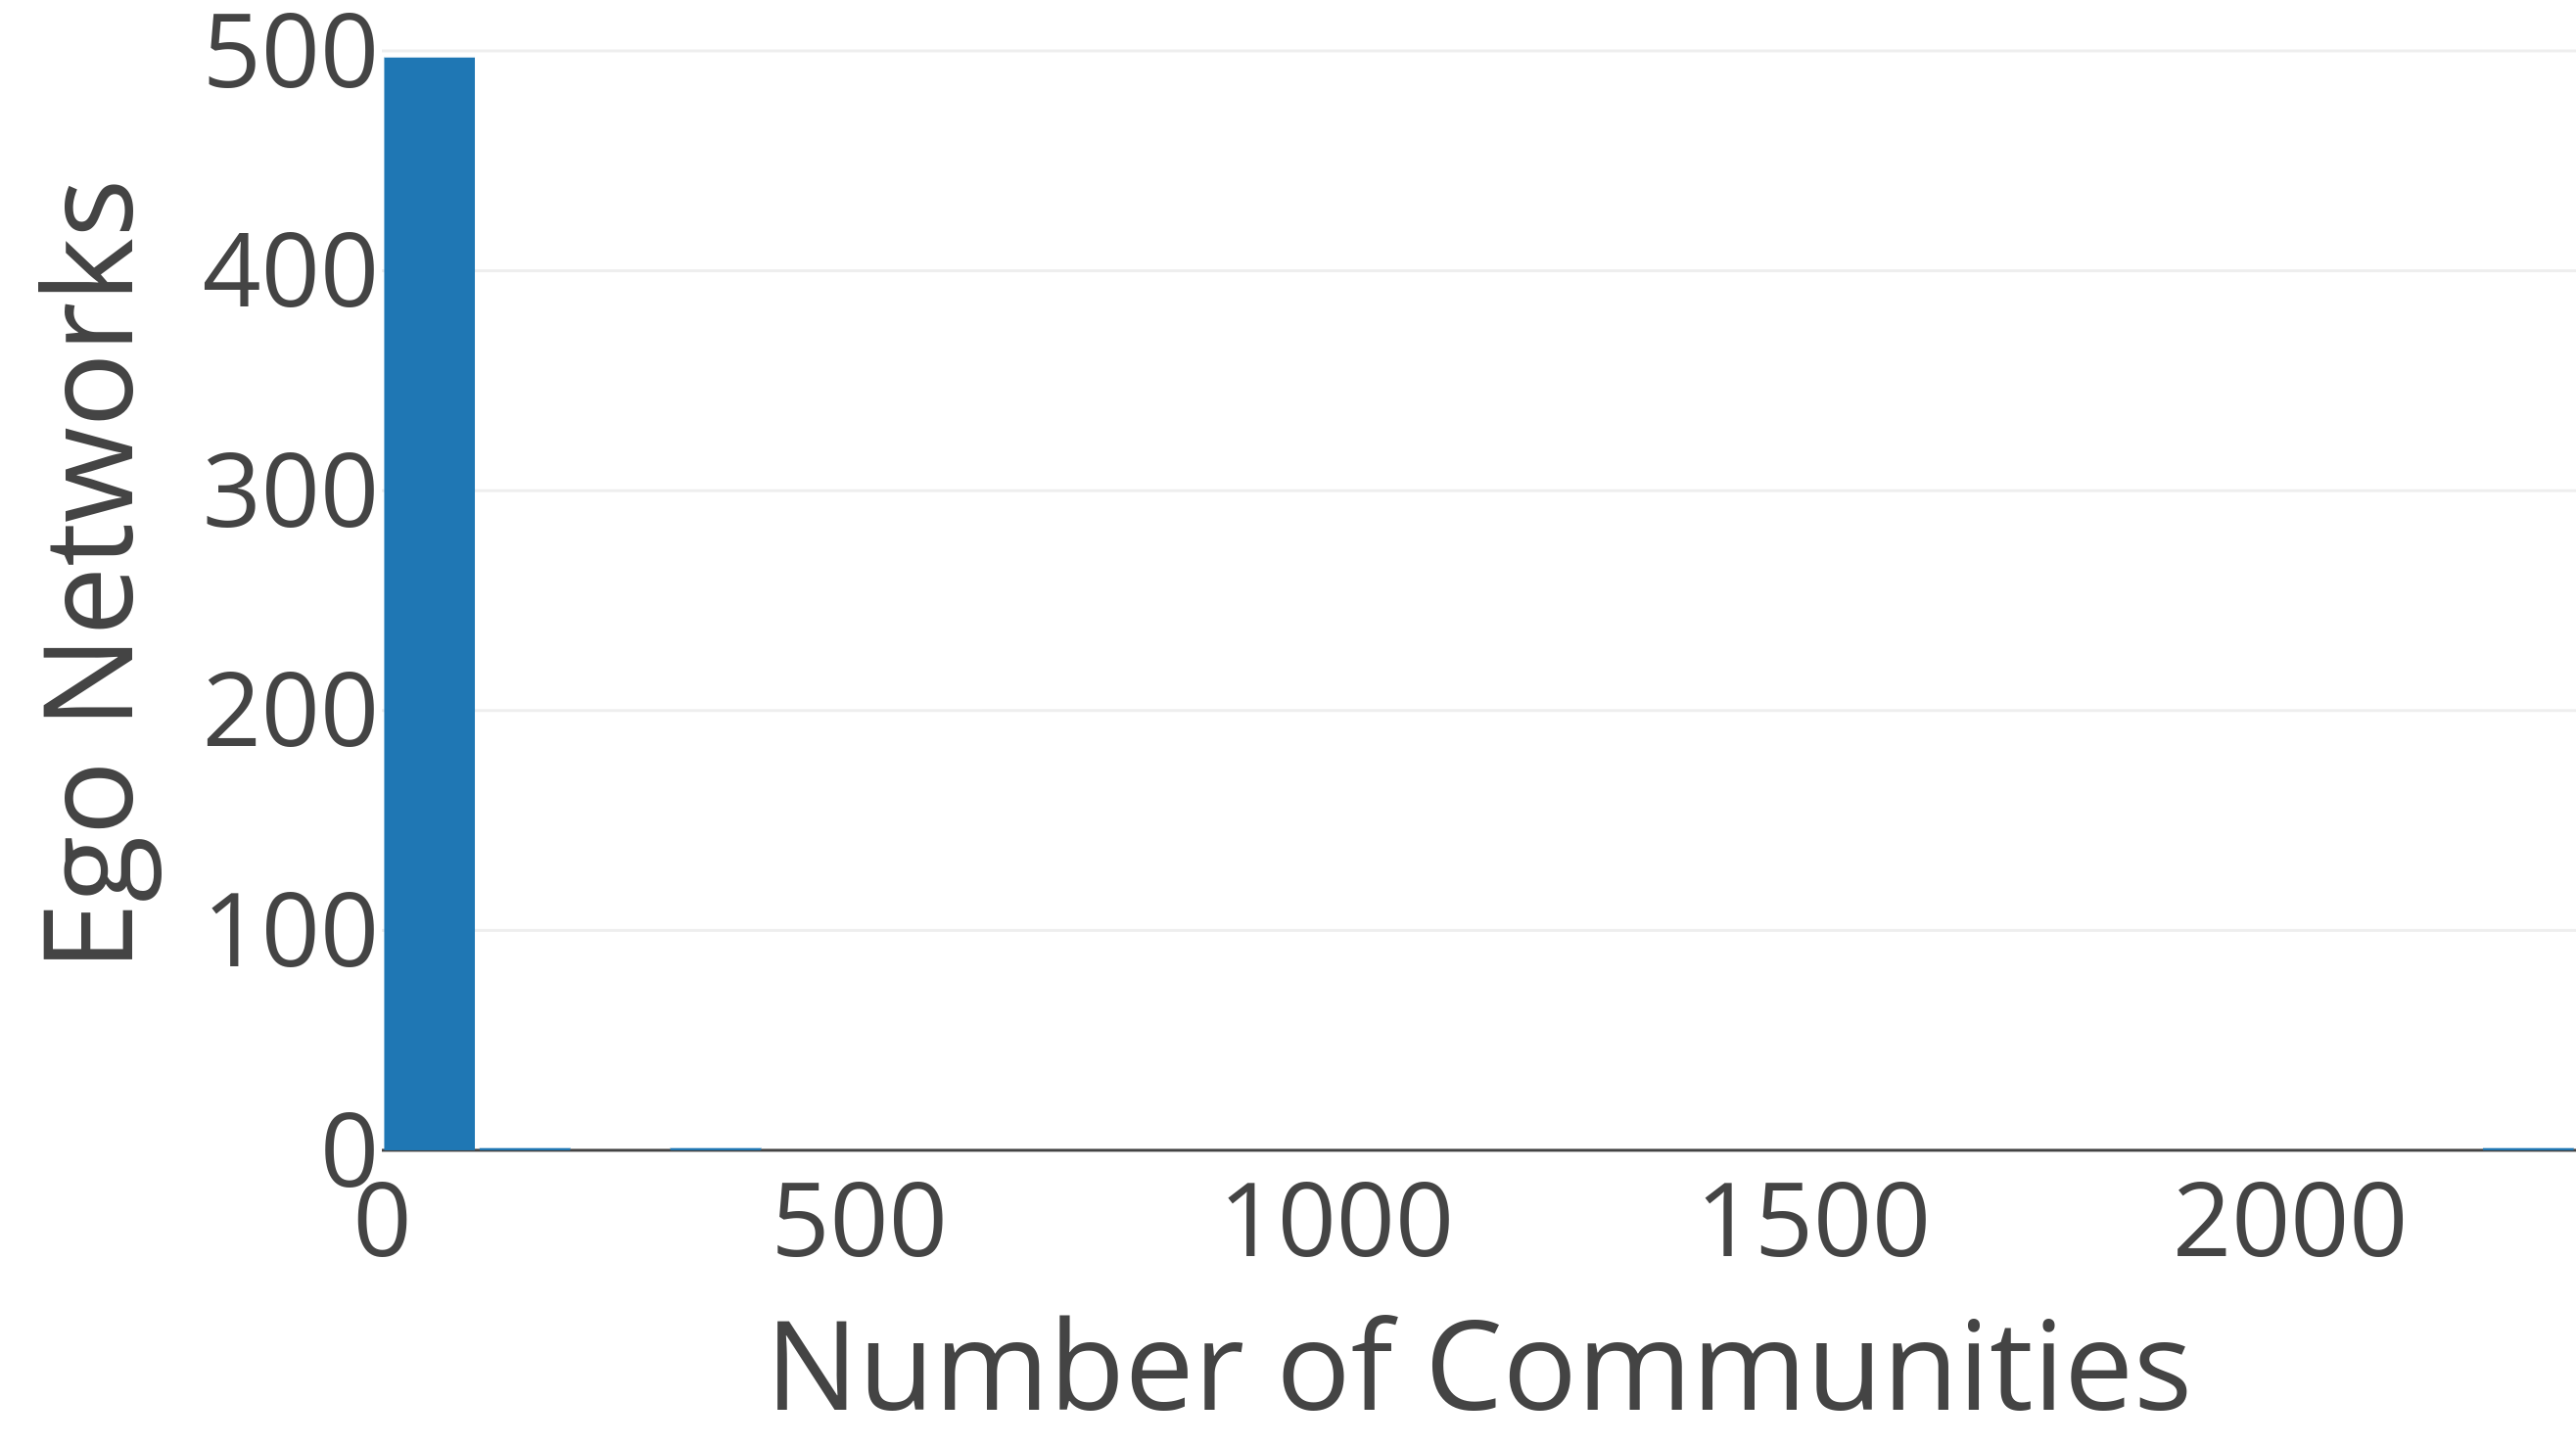
\includegraphics[width=0.47\textwidth]{fig/comm_stats/copra/n_comm/n_comm_copra_follow.png}
        \label{fig:comm_stats_n_comm_copra_follow}
    }
    \subfigure[Retweet]{
        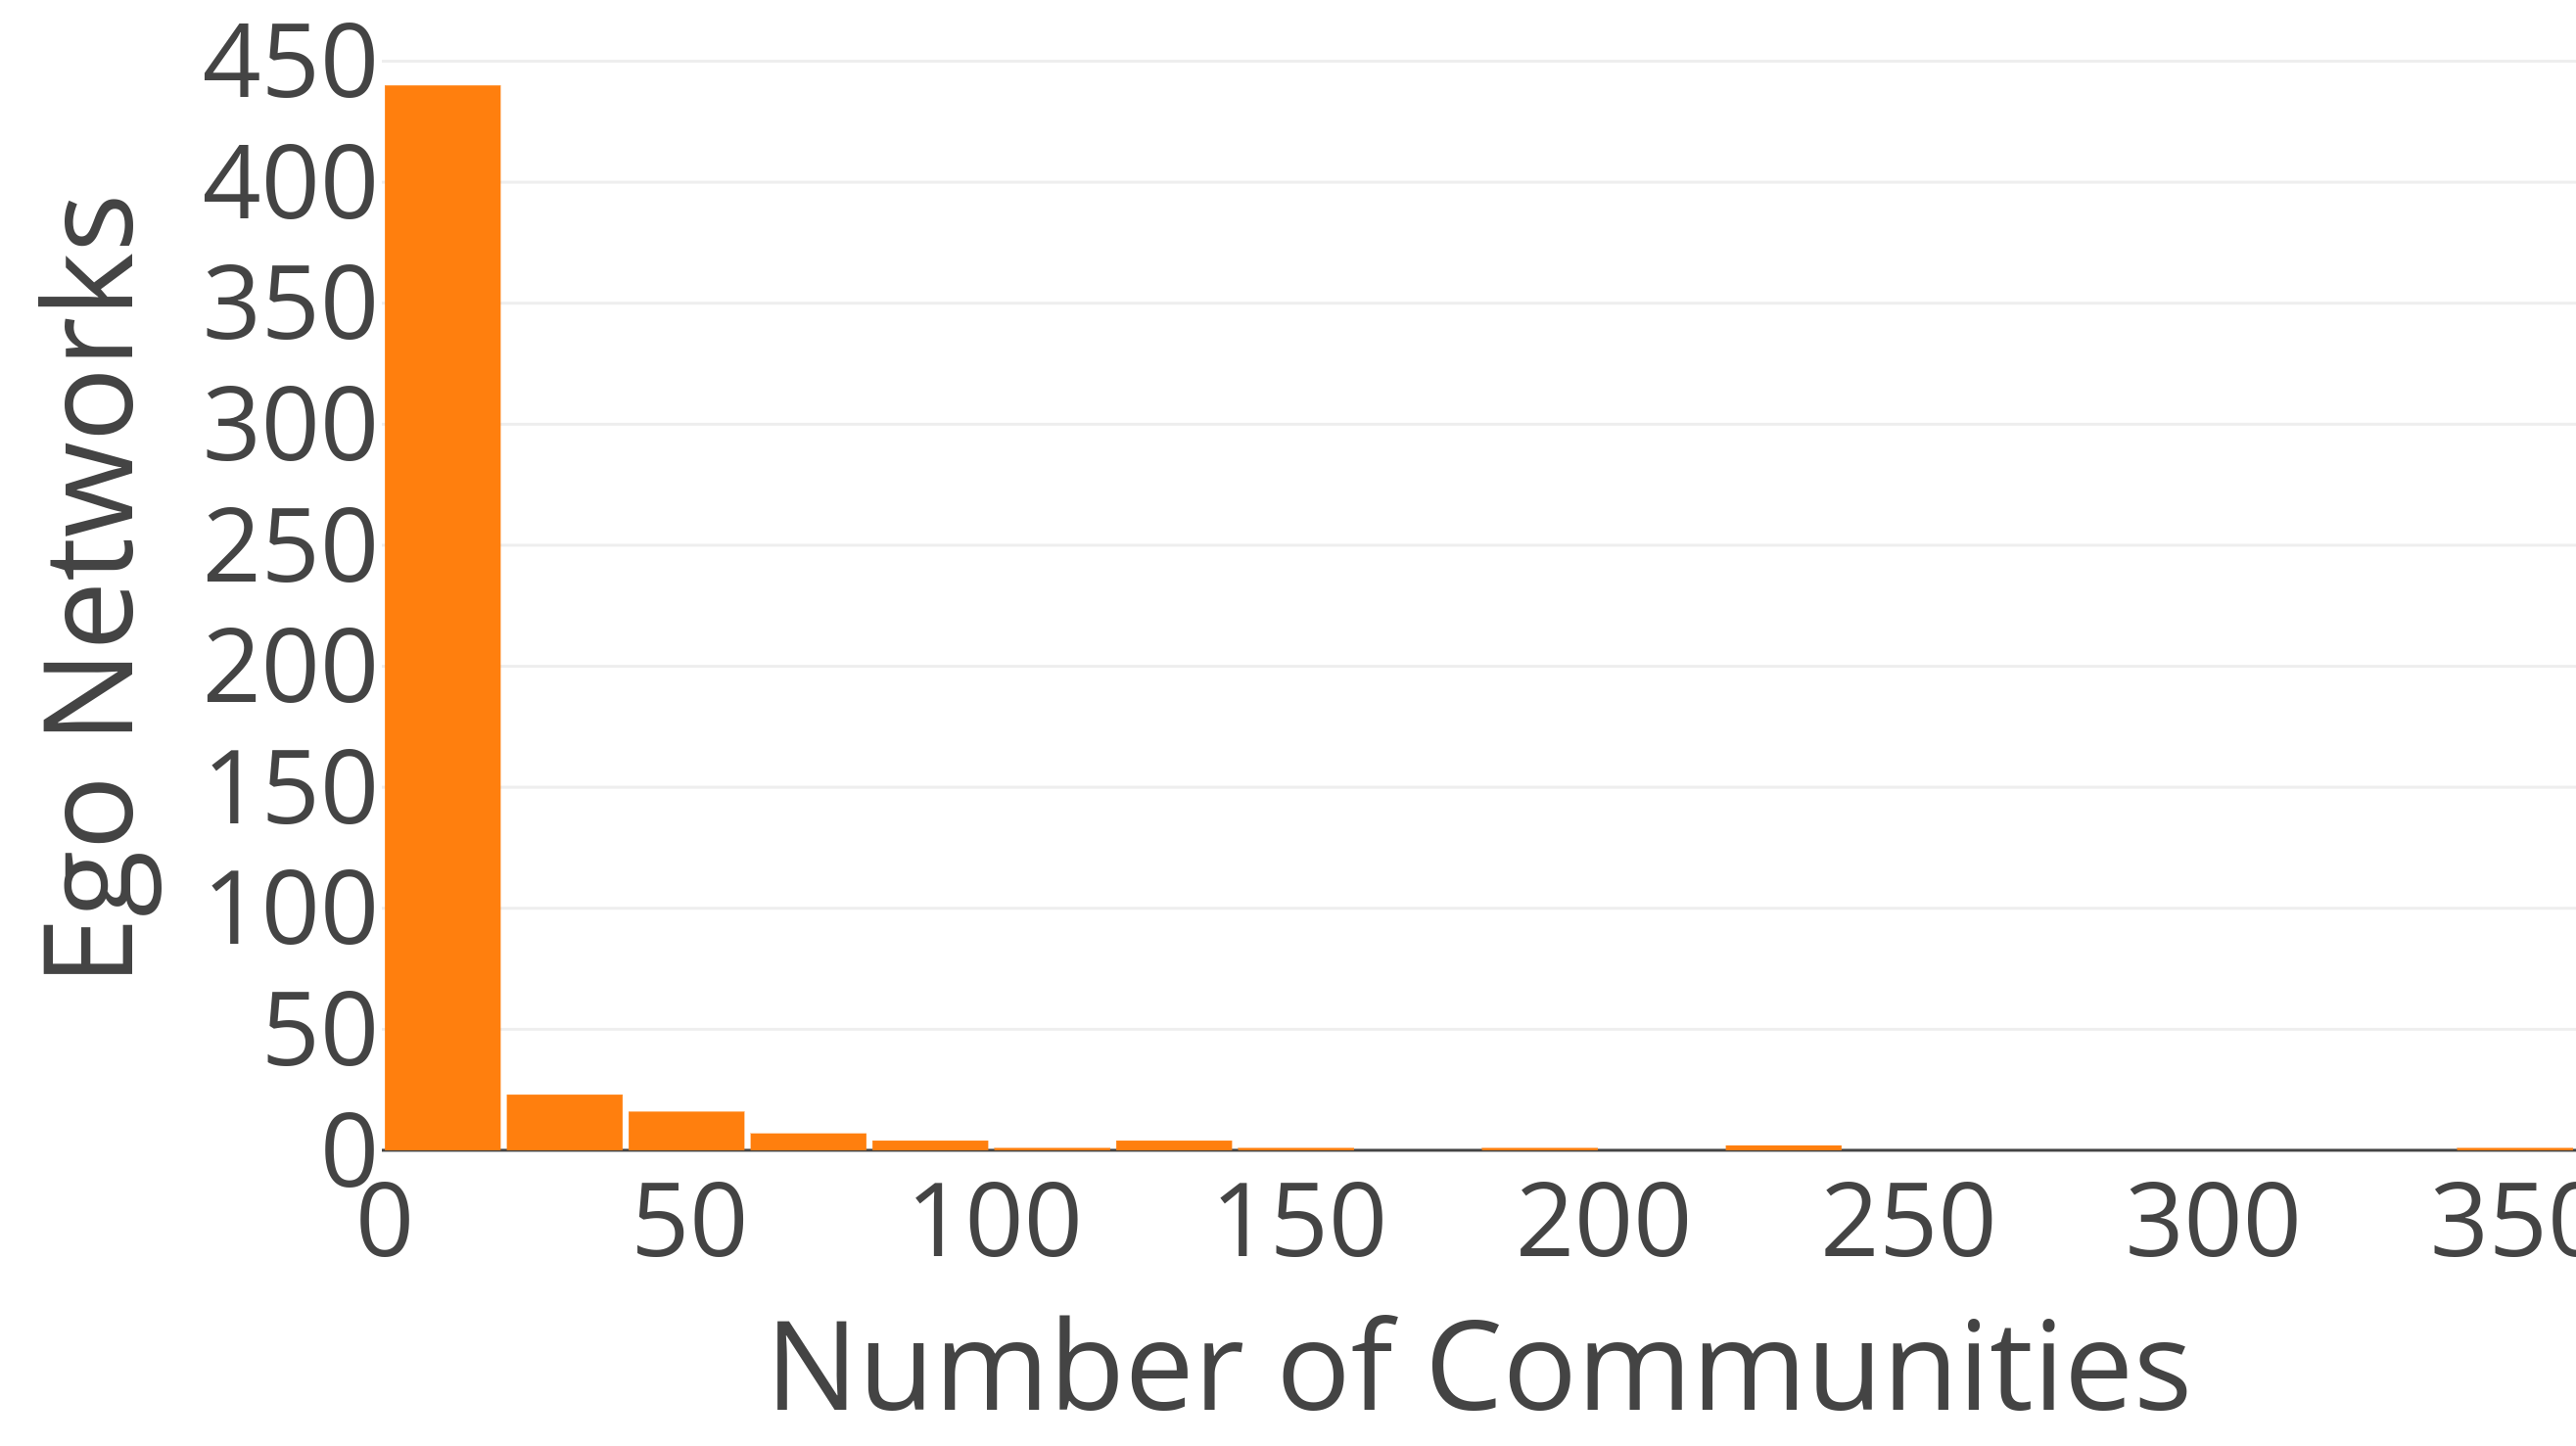
\includegraphics[width=0.47\textwidth]{fig/comm_stats/copra/n_comm/n_comm_copra_retweet.png}
        \label{fig:comm_stats_n_comm_copra_retweet}
    } \\
    \subfigure[Like]{
        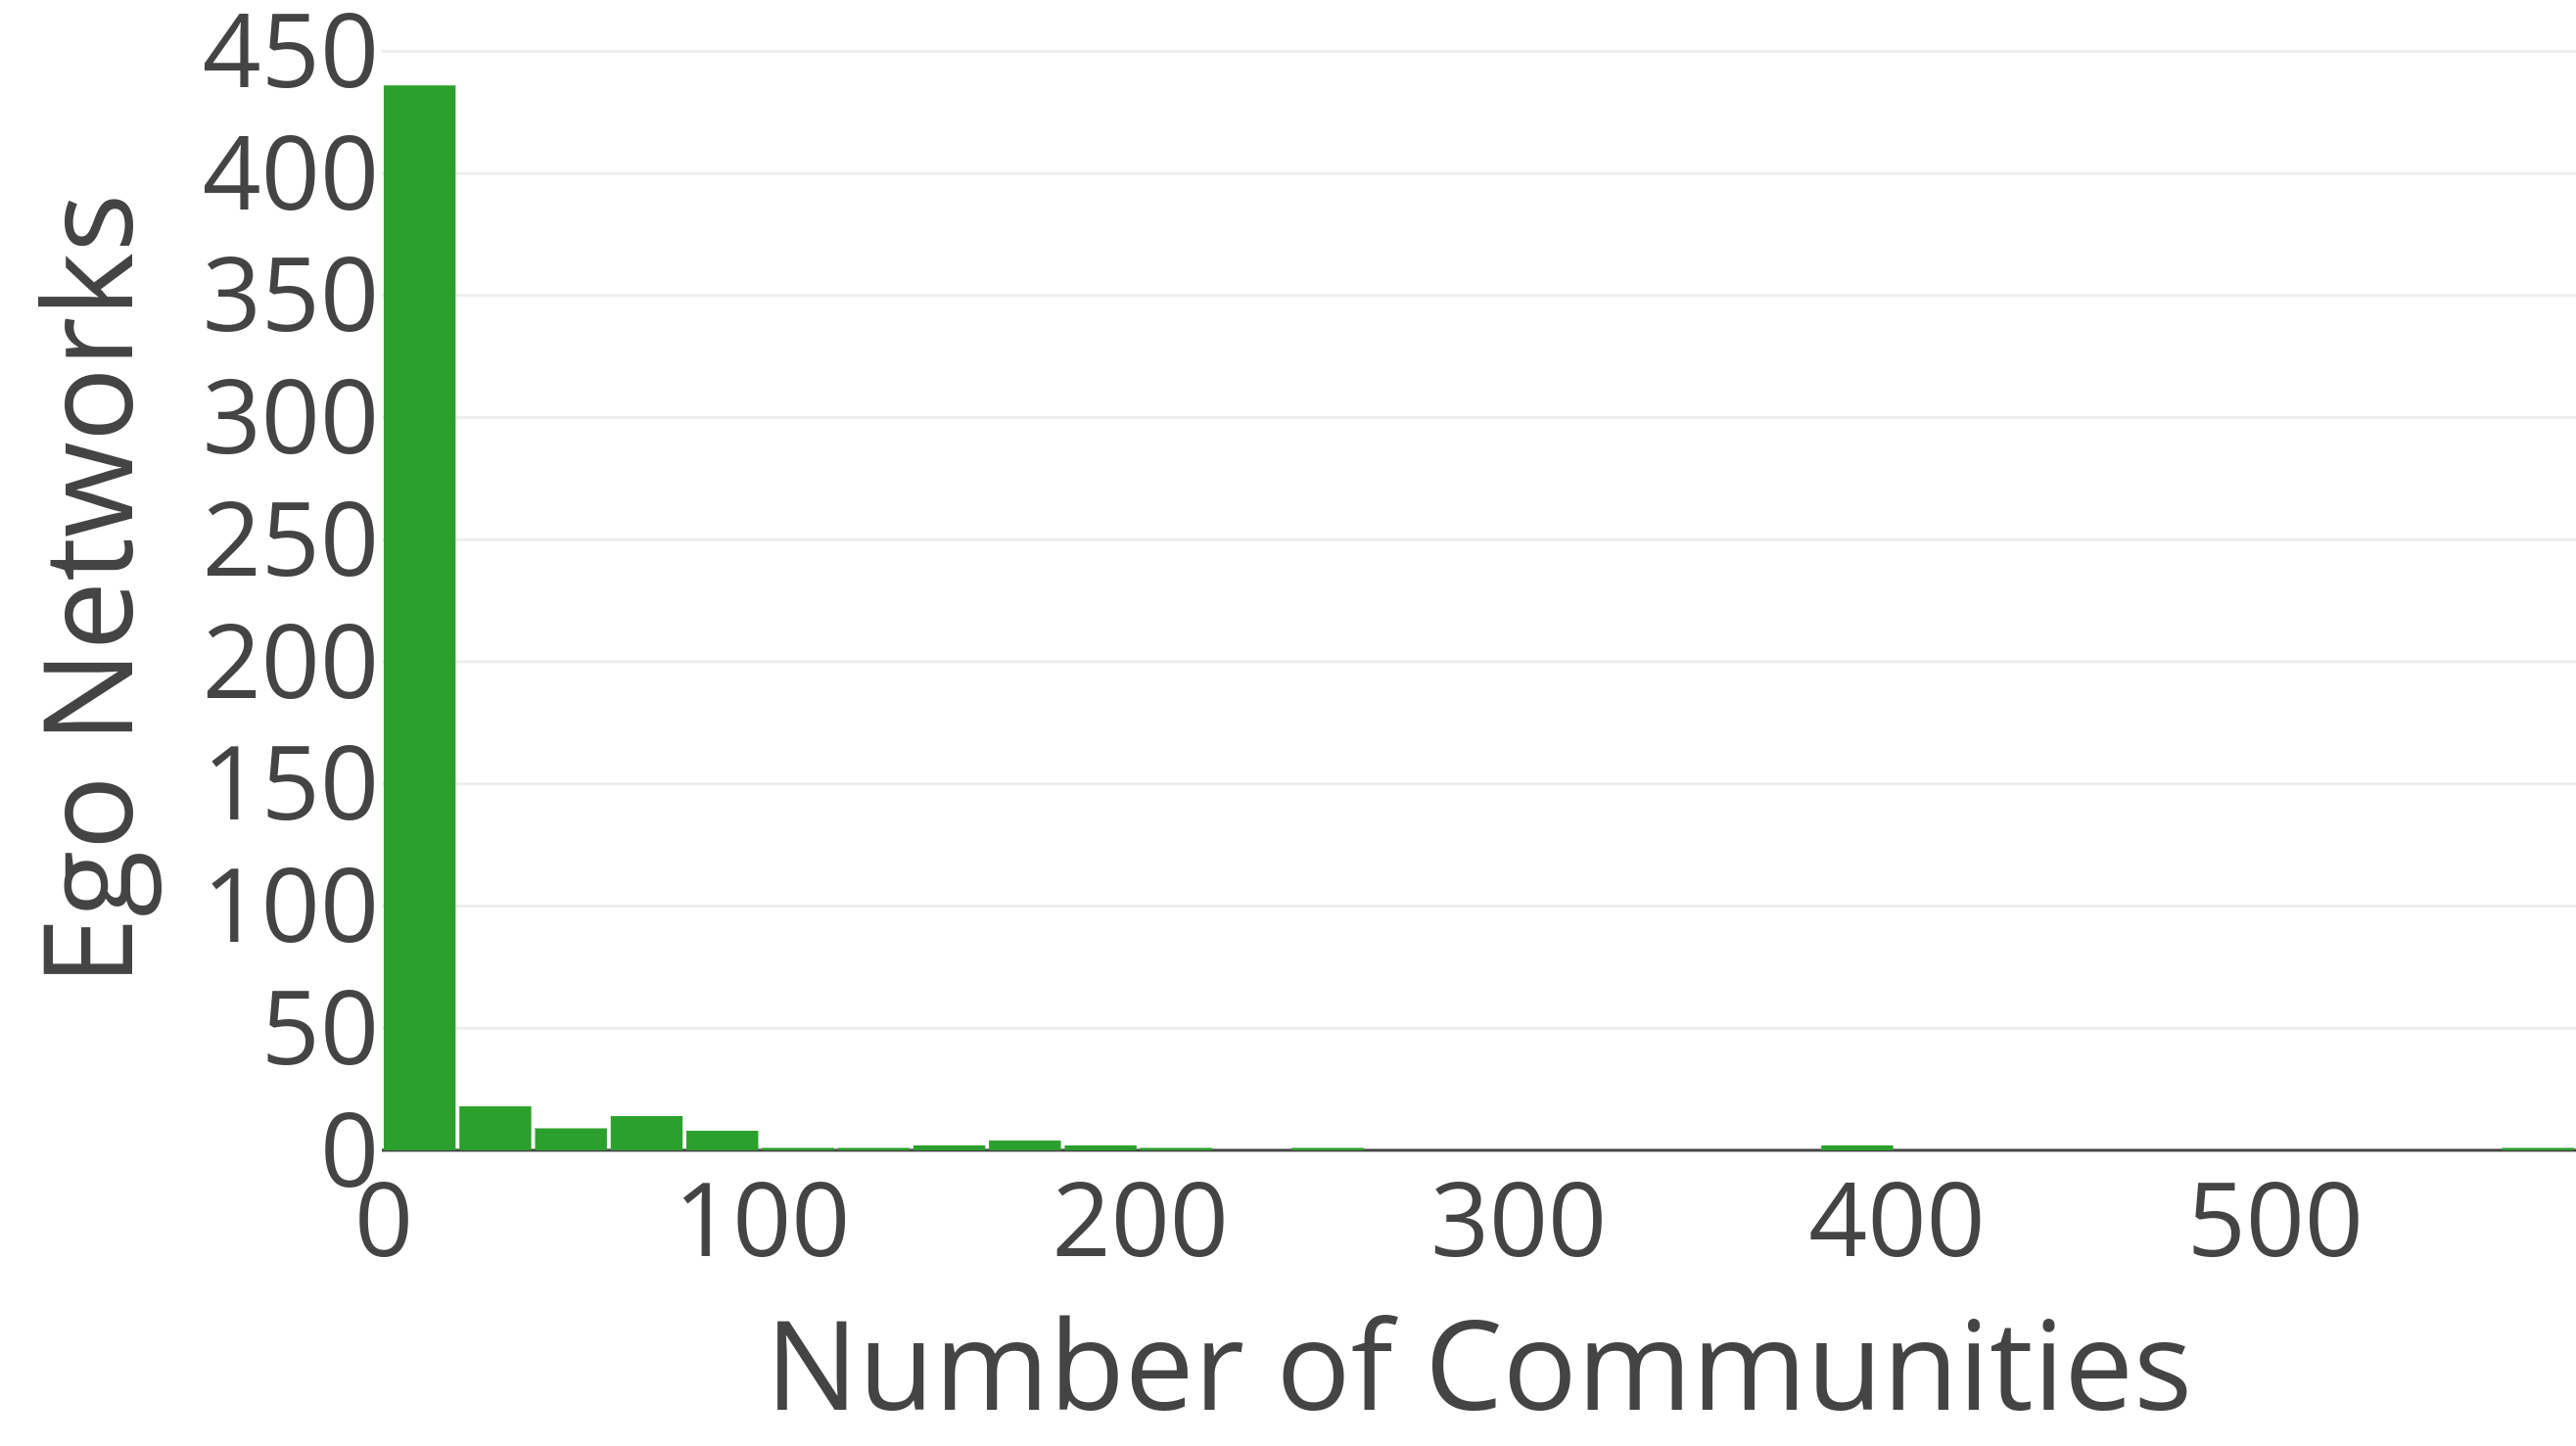
\includegraphics[width=0.47\textwidth]{fig/comm_stats/copra/n_comm/n_comm_copra_like.png}
        \label{fig:comm_stats_n_comm_copra_like}
    }
    \subfigure[Mention]{
        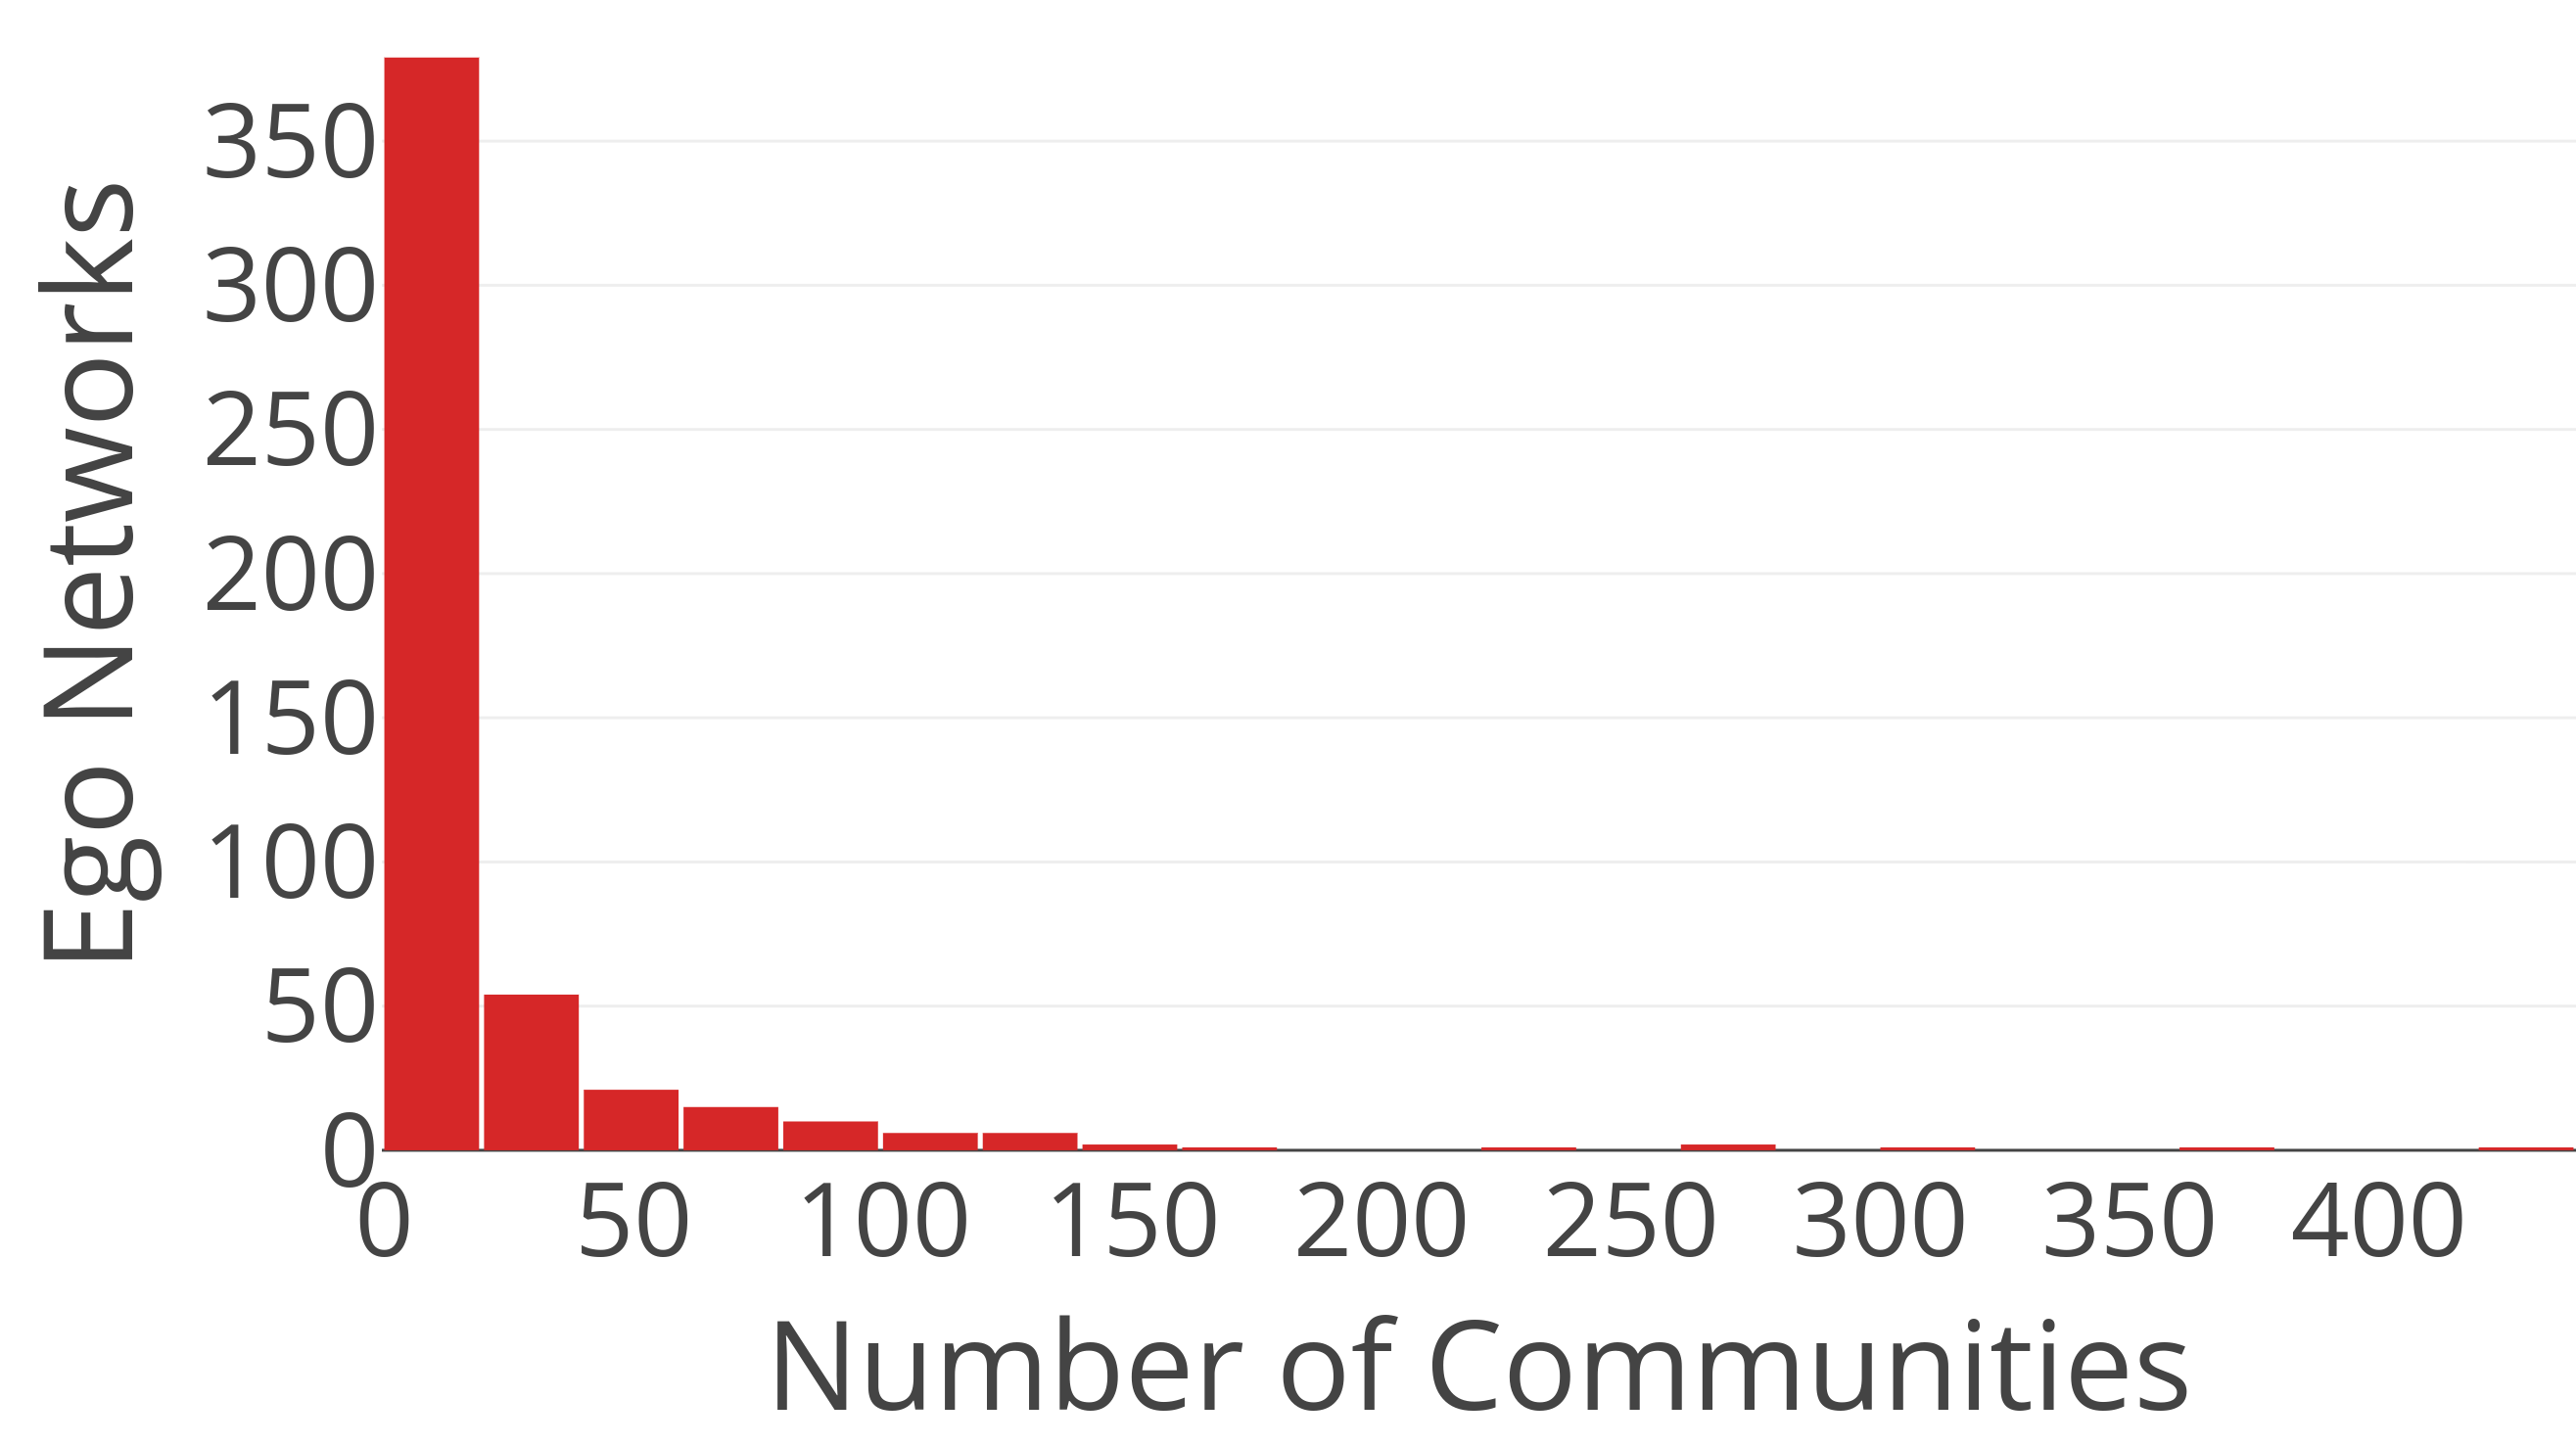
\includegraphics[width=0.47\textwidth]{fig/comm_stats/copra/n_comm/n_comm_copra_mention.png}
        \label{fig:comm_stats_n_comm_copra_mention}
    }
    \caption{Number of communities detected by COPRA.}
    \label{fig:comm_stats_n_comm_copra}
\end{figure}
\begin{figure}[h!tb]
    \centering
    \subfigure[Follow]{
        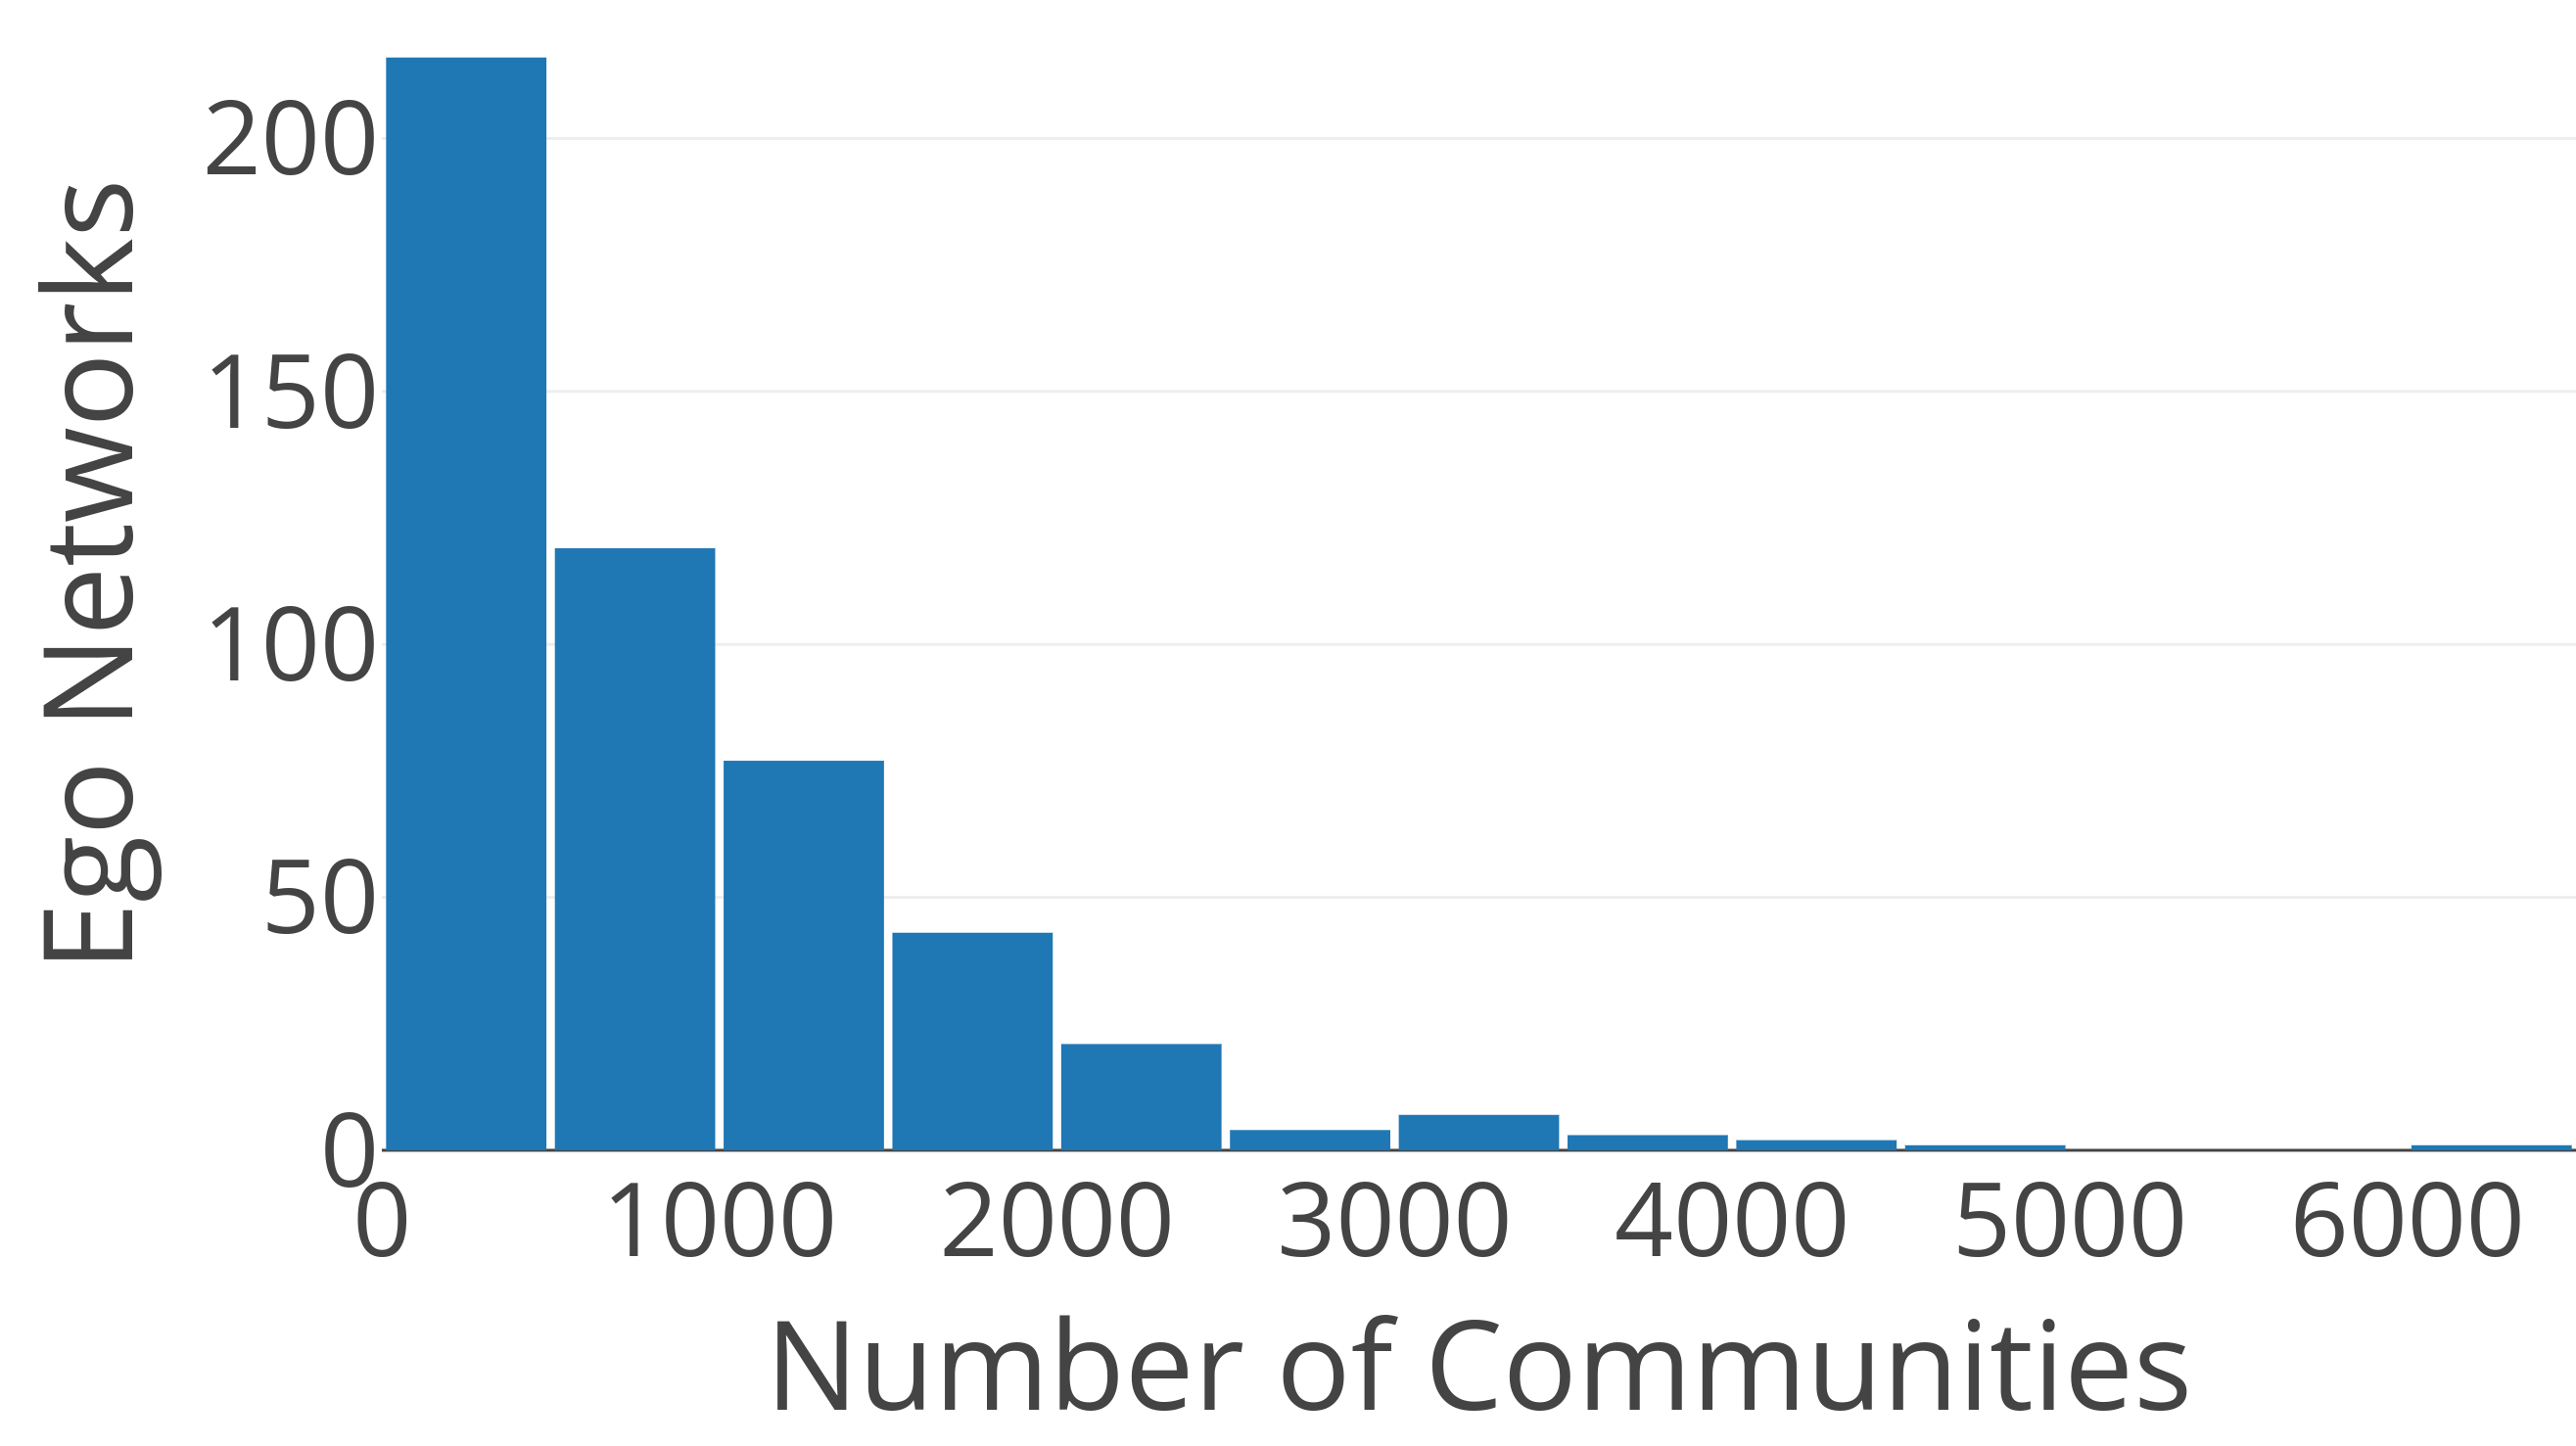
\includegraphics[width=0.47\textwidth]{fig/comm_stats/oslom/n_comm/n_comm_oslom_follow.png}
        \label{fig:comm_stats_n_comm_oslom_follow}
    }
    \subfigure[Retweet]{
        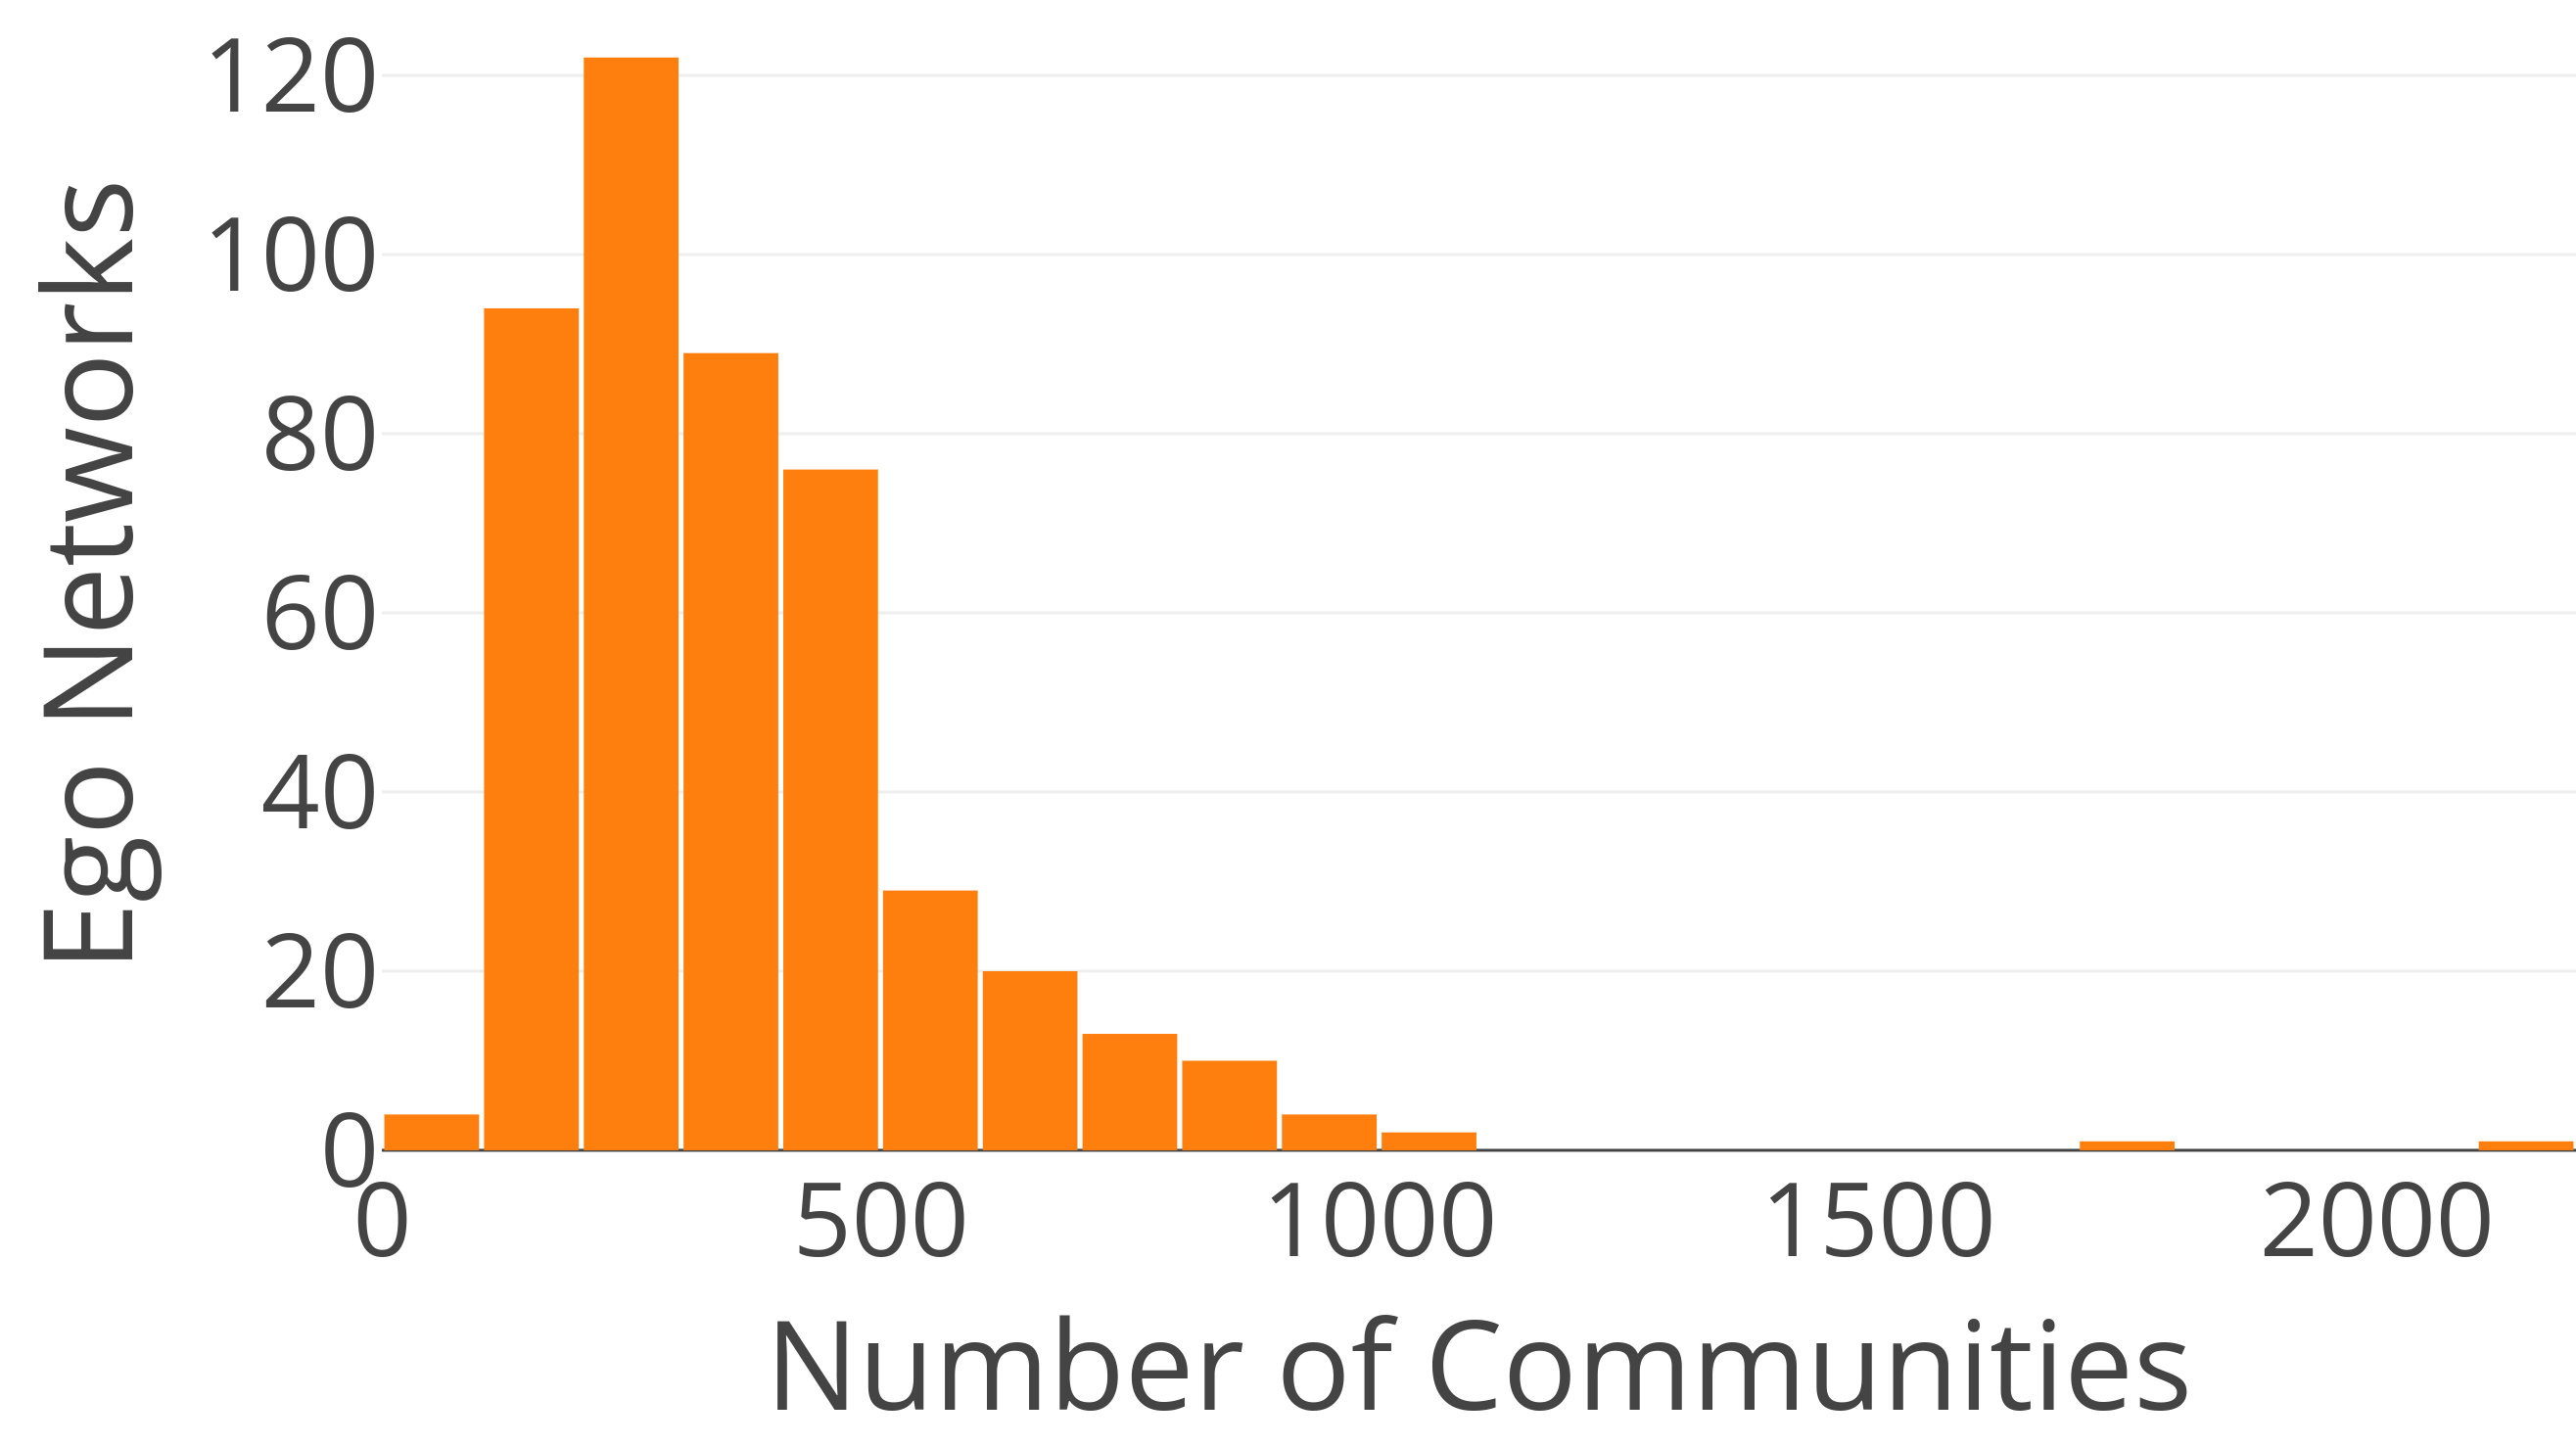
\includegraphics[width=0.47\textwidth]{fig/comm_stats/oslom/n_comm/n_comm_oslom_retweet.png}
        \label{fig:comm_stats_n_comm_oslom_retweet}
    } \\
    \subfigure[Like]{
        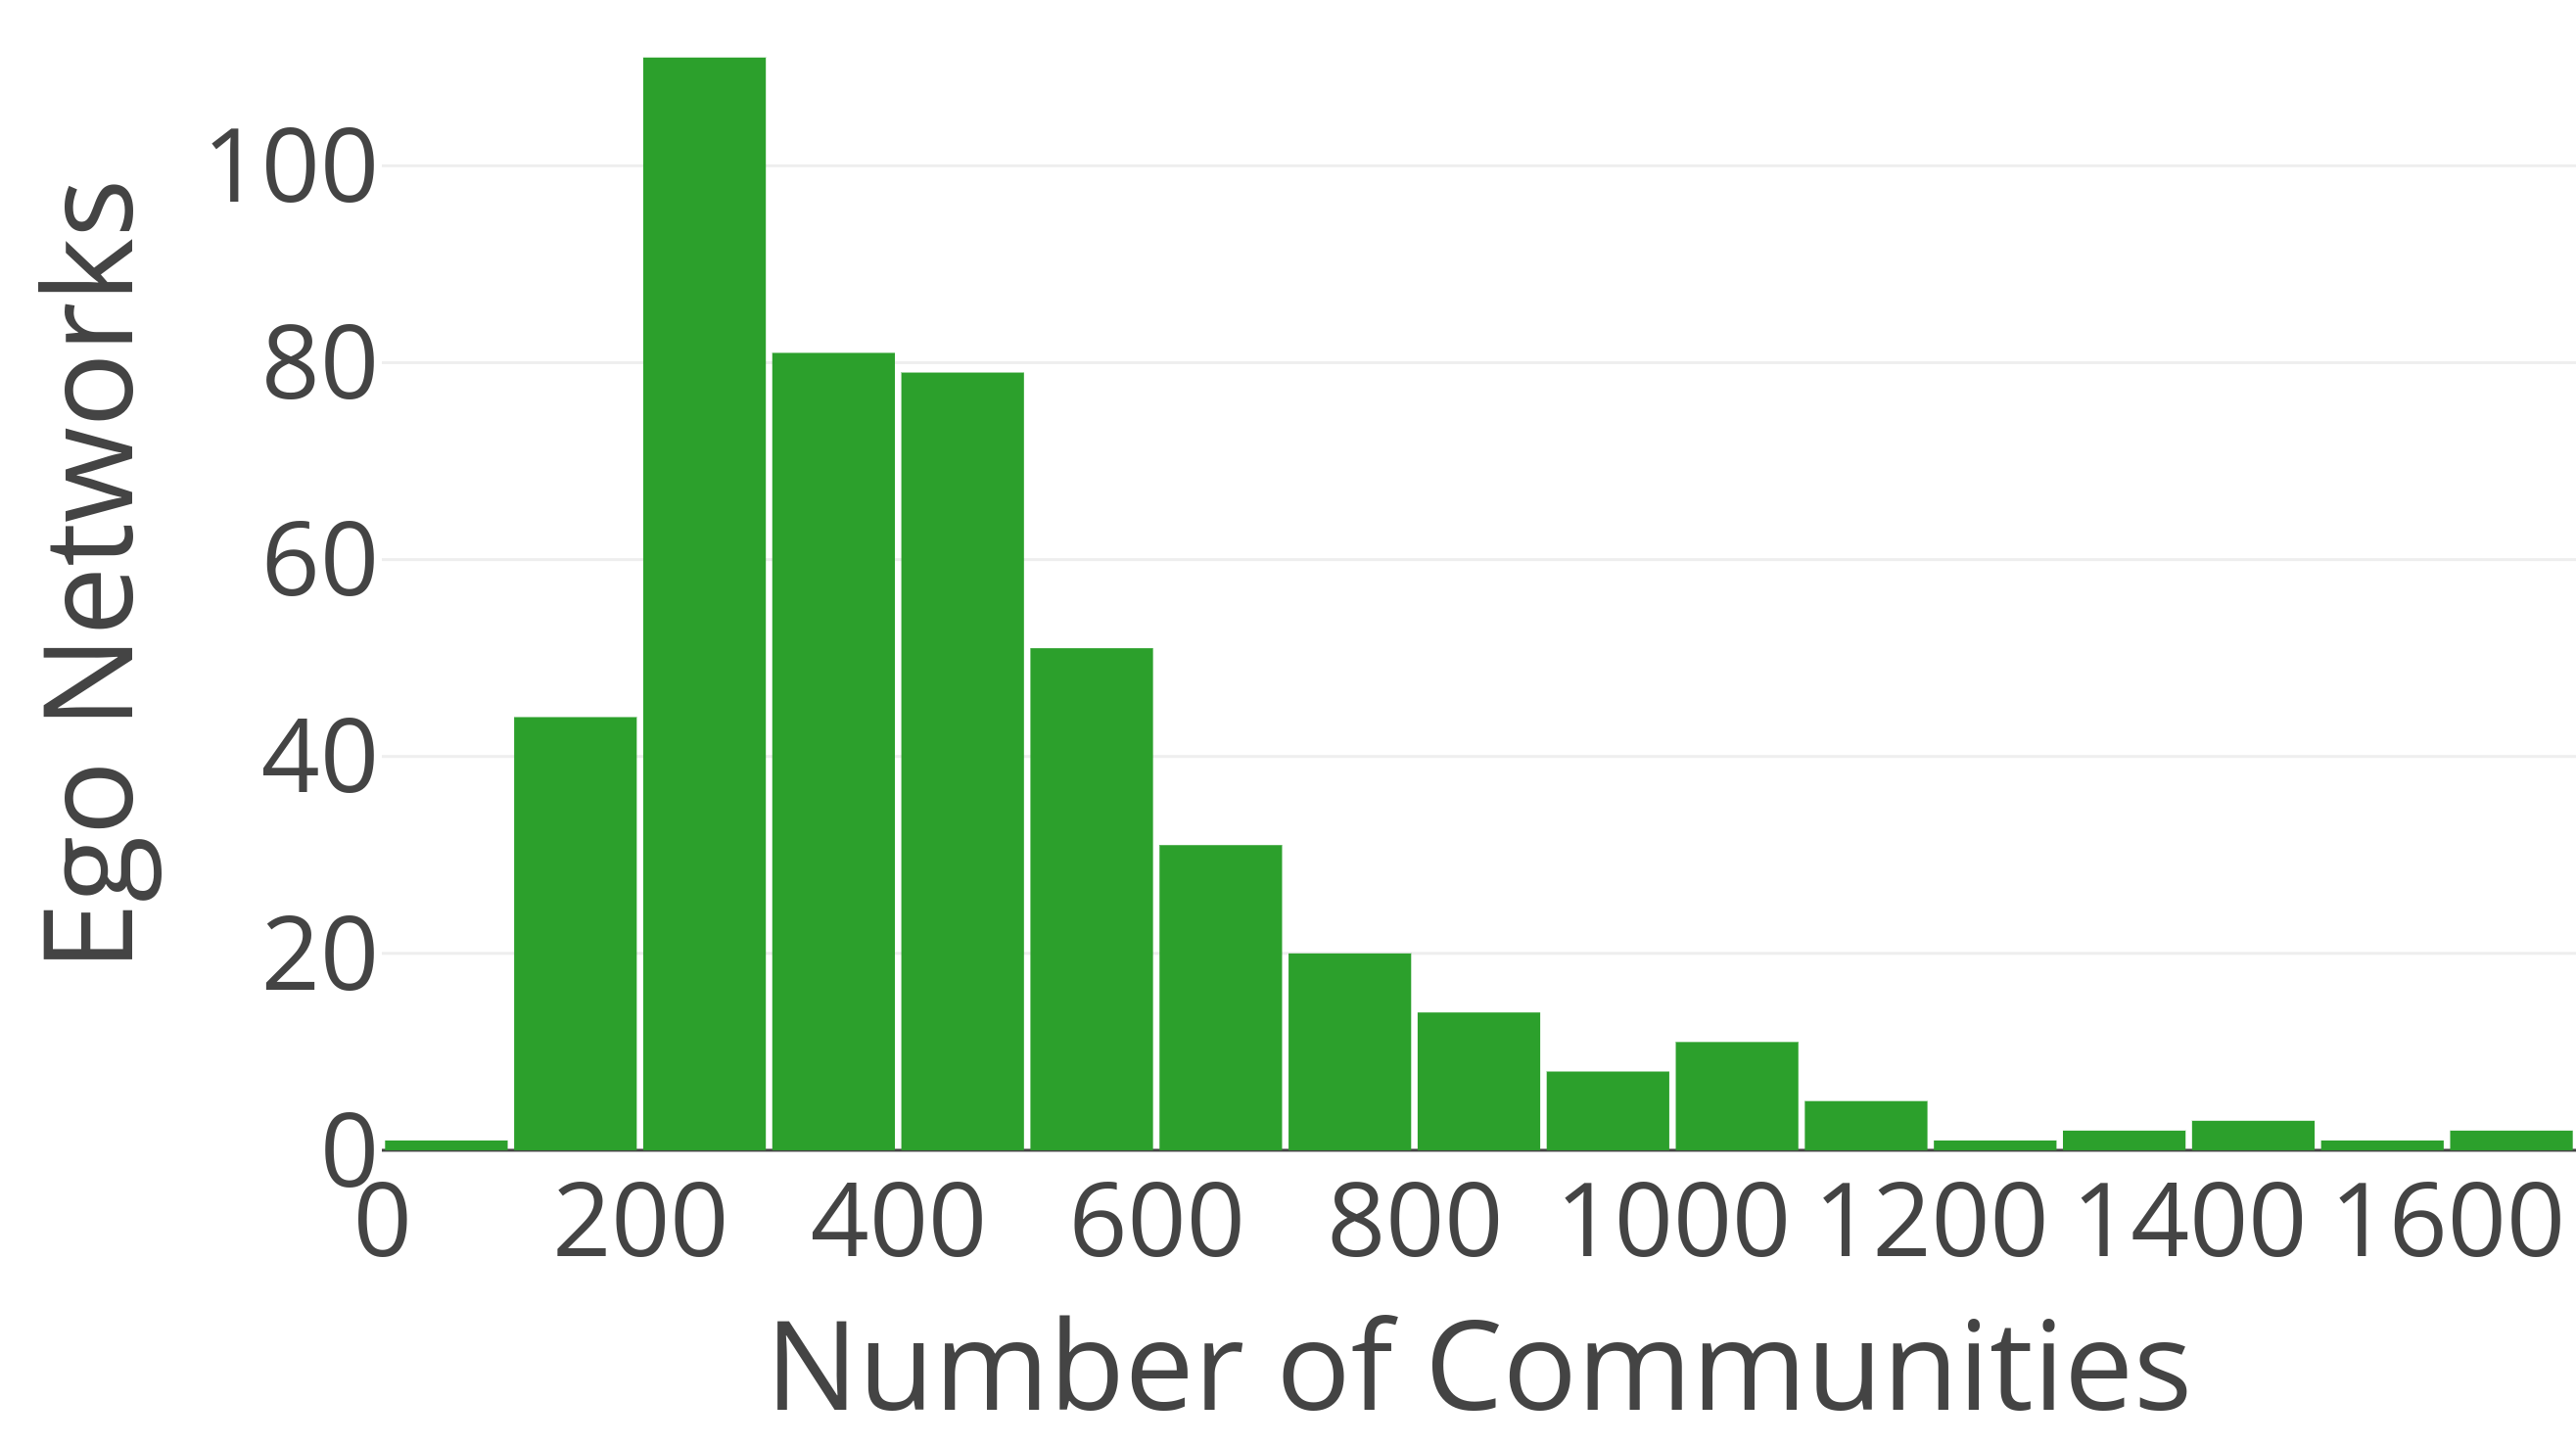
\includegraphics[width=0.47\textwidth]{fig/comm_stats/oslom/n_comm/n_comm_oslom_like.png}
        \label{fig:comm_stats_n_comm_oslom_like}
    }
    \subfigure[Mention]{
        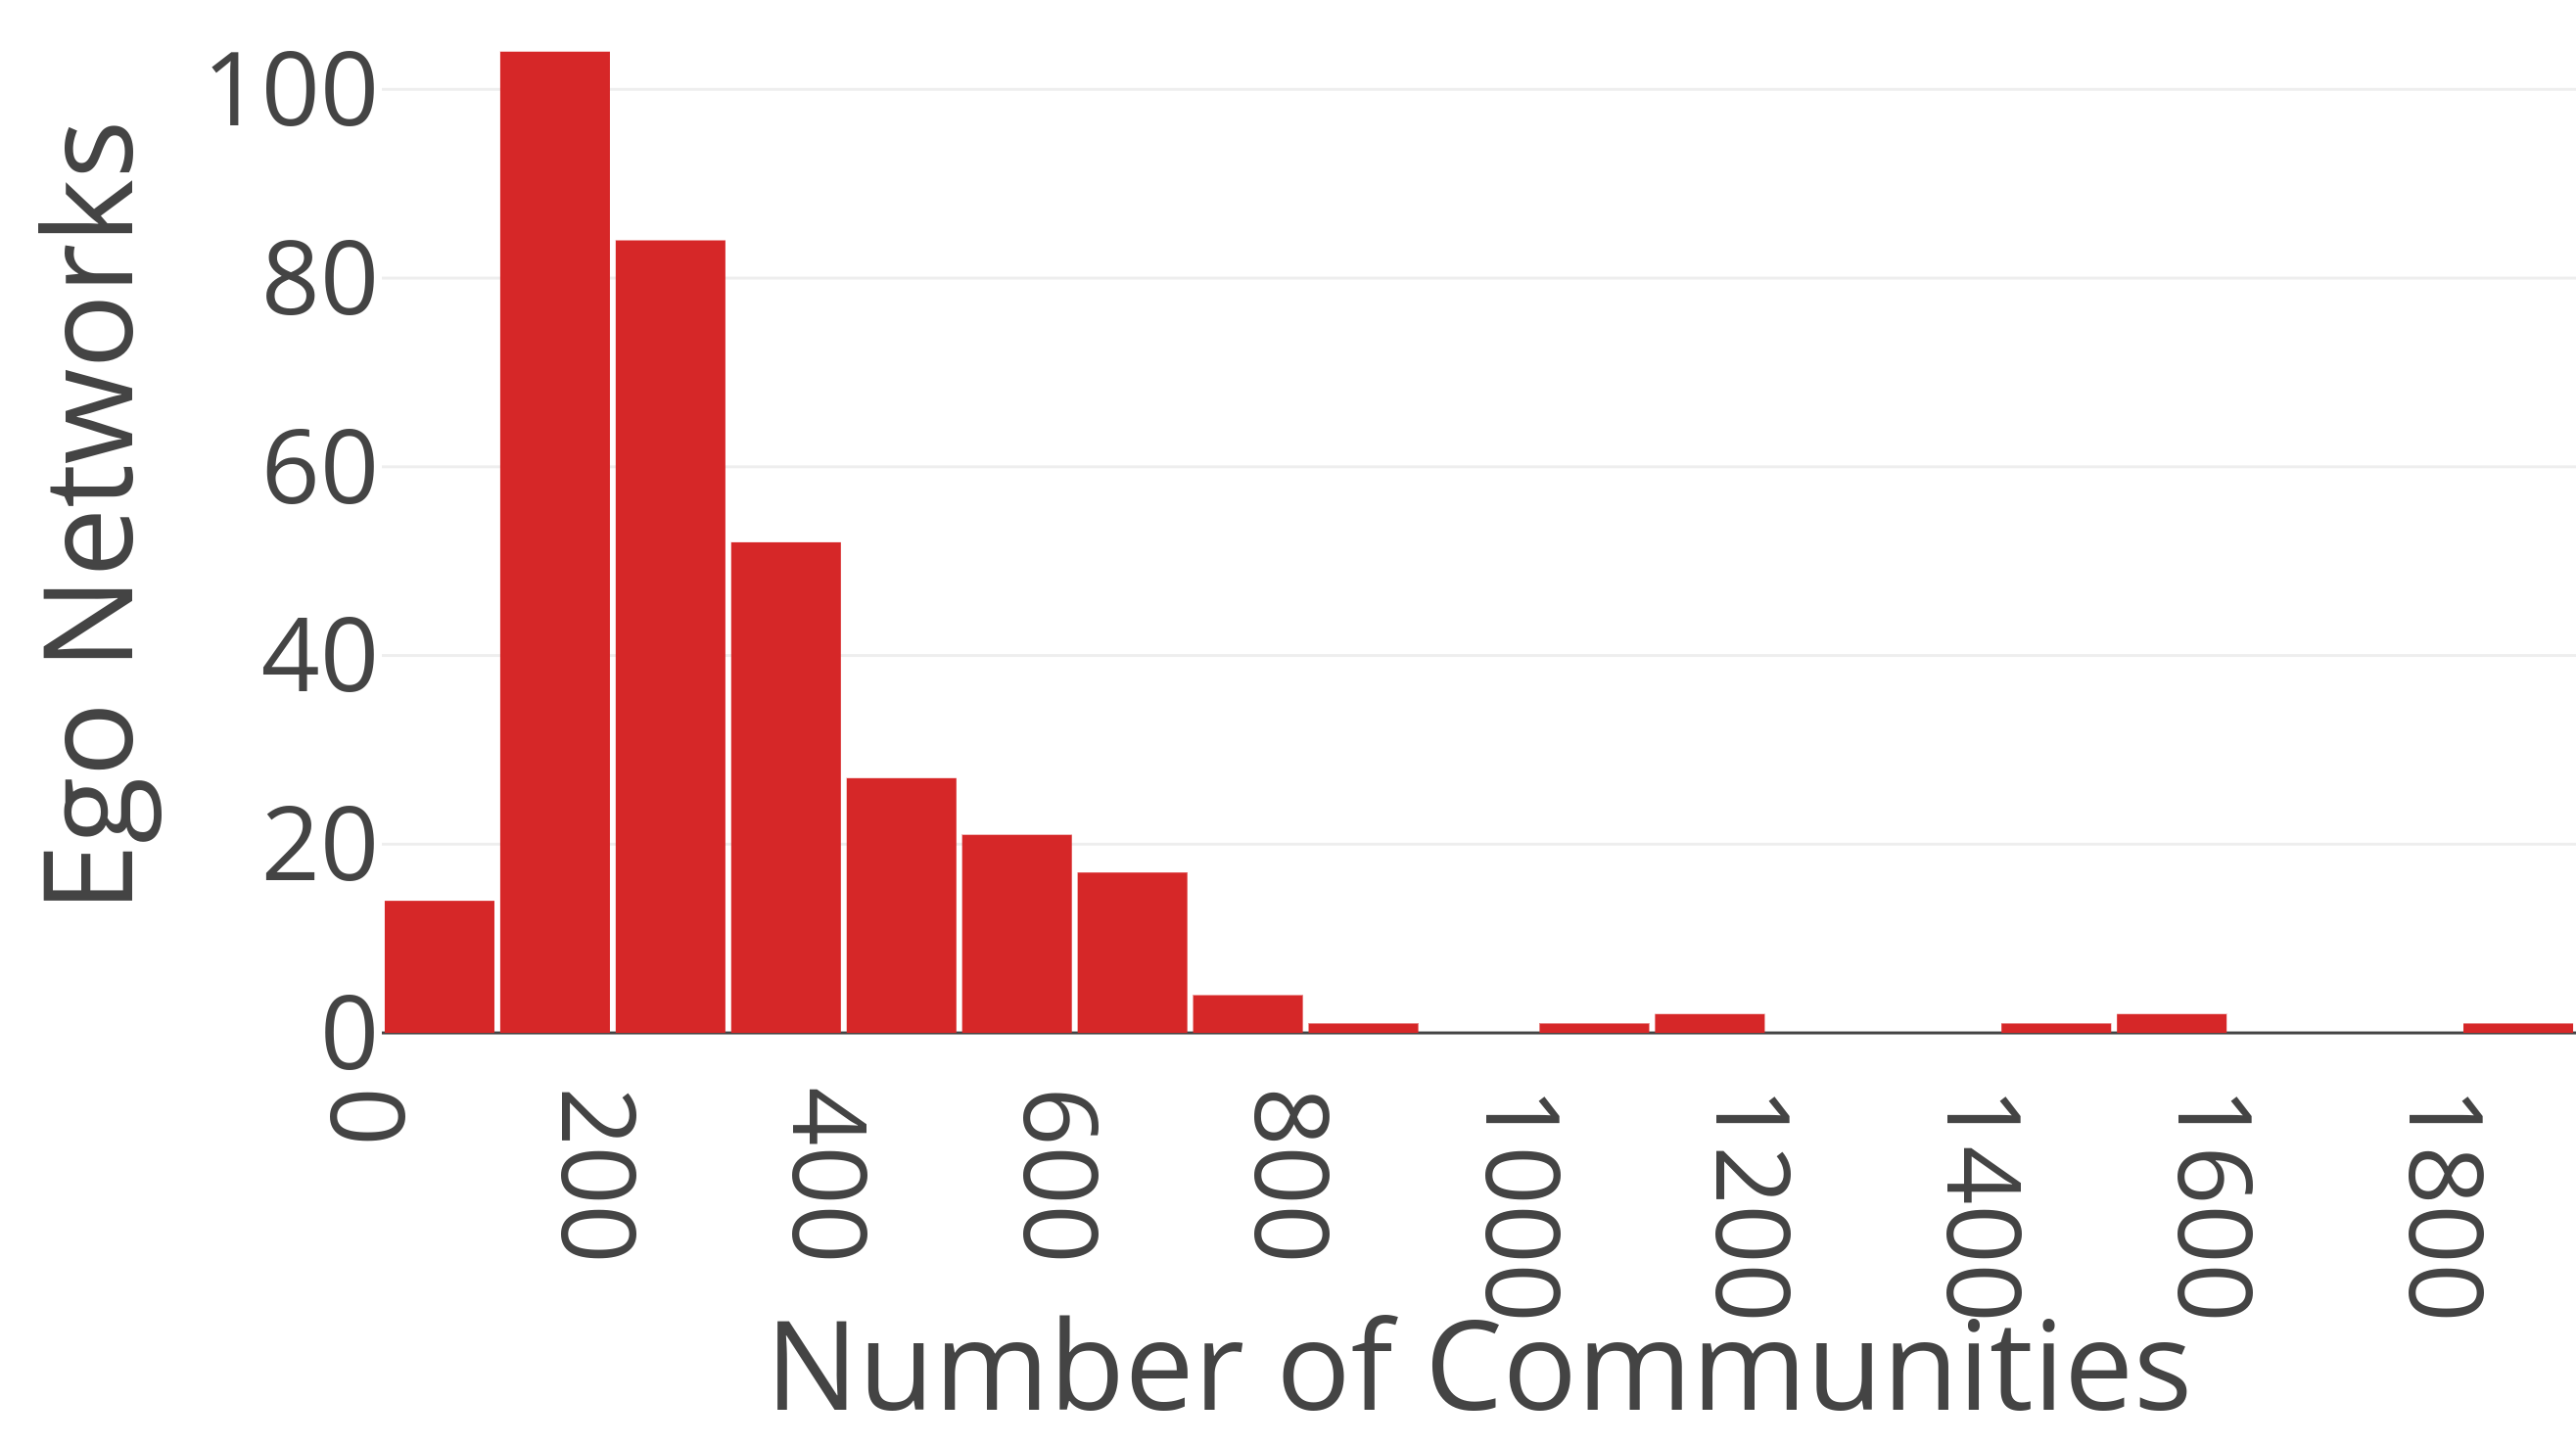
\includegraphics[width=0.47\textwidth]{fig/comm_stats/oslom/n_comm/n_comm_oslom_mention.png}
        \label{fig:comm_stats_n_comm_oslom_mention}
    }
    \caption{Number of communities detected by OSLOM.}
    \label{fig:comm_stats_n_comm_oslom}
\end{figure}

We compute the number of communities detected by each algorithm in each of the layers of all ego networks. The results are presented in figures \ref{fig:comm_stats_n_comm_rak}, \ref{fig:comm_stats_n_comm_infomap}, \ref{fig:comm_stats_n_comm_copra} and \ref{fig:comm_stats_n_comm_oslom} through histograms with the frequency distribution of the detected communities. The results indicate that the vertices of all the layers of the analyzed ego networks have similar behavior. For the algorithms INFOMAP and OSLOM, the vertices tend to form communities, and for the RAK and COPRA algorithms the networks themselves, or at least most of the vertices of the ego network, are considered as a single community.

The Fig. \ref{fig:comm_stats_n_comm_rak} shows a histogram with the frequency distribution of the number of communities detected by the algorithm RAK. For most egos networks this algorithm detected few communities at all layers, while few ego networks exhibit a high number of communities. Fig. \ref{fig:comm_stats_n_comm_infomap} shows a histogram for the number of communities detected by the INFOMAP algorithm. Unlike RAK, INFOMAP detects a greater number of communities for all layers. Fig. \ref{fig:comm_stats_n_comm_copra} shows a plot with the number of communities detected by the COPRA algorithm, and the results are very similar to those found with the RAK algorithm. Fig. \ref{fig:comm_stats_n_comm_oslom} shows the number of communities detected with the OSLOM algorithm, which is the algorithm that can identify the largest number of communities, but it is worth remembering that the COPRA and OSLOM algorithms detect overlap, that is to say that a vertex can be associated with more than one community.

%However, INFOMAP presented the best average values for most community evaluation measures considered in Section \ref{sec:comm_quality}, thus we report only INFOMAP results  in this work. We have that the sizes of the communities vary greatly inside a layer for a given ego. In the great majority of the cases the mean size of the communities is  much smaller than the standard deviation. In most cases the biggest community is much greater than the mean sizes and the smallest contains only one alter. 

\begin{figure}[h!tb]
    \centering
    \subfigure[RAK]{
        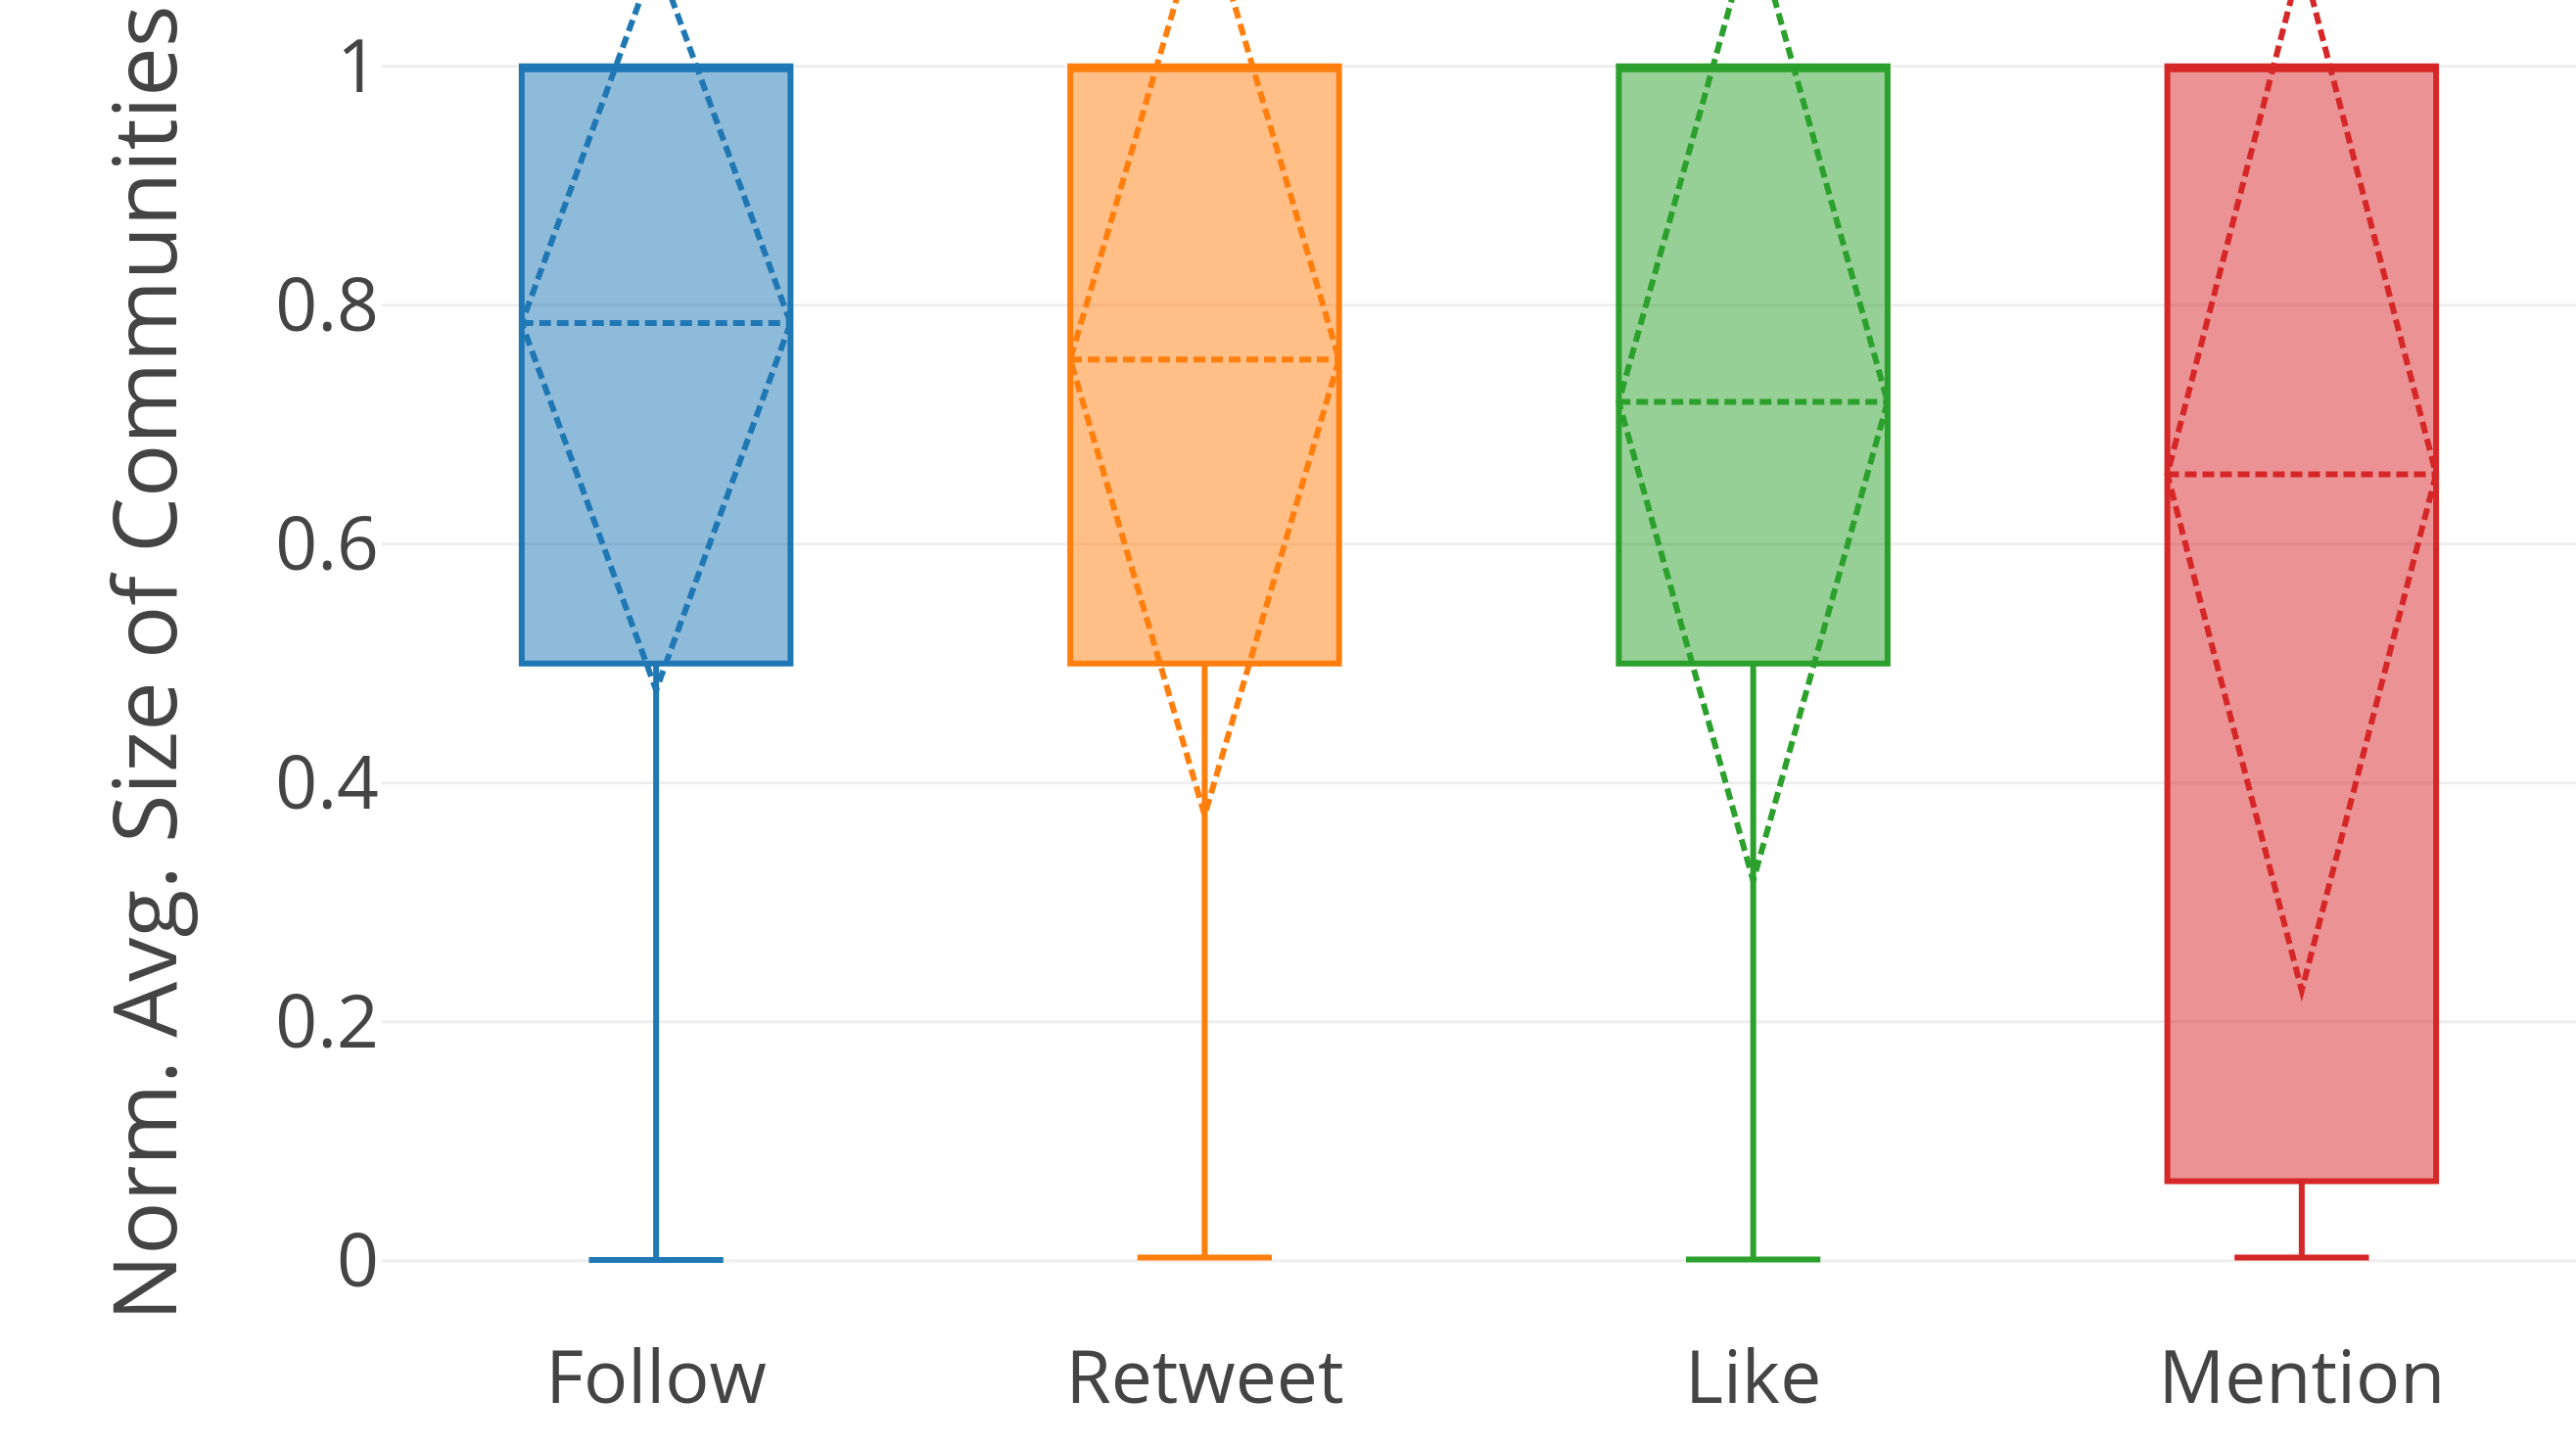
\includegraphics[width=0.47\textwidth]{fig/comm_stats/rak/comm_stats_norm_avg_comm_rak.png}
        \label{fig:comm_stats_avg_size_comm_rak}
    }
    \subfigure[INFOMAP]{
        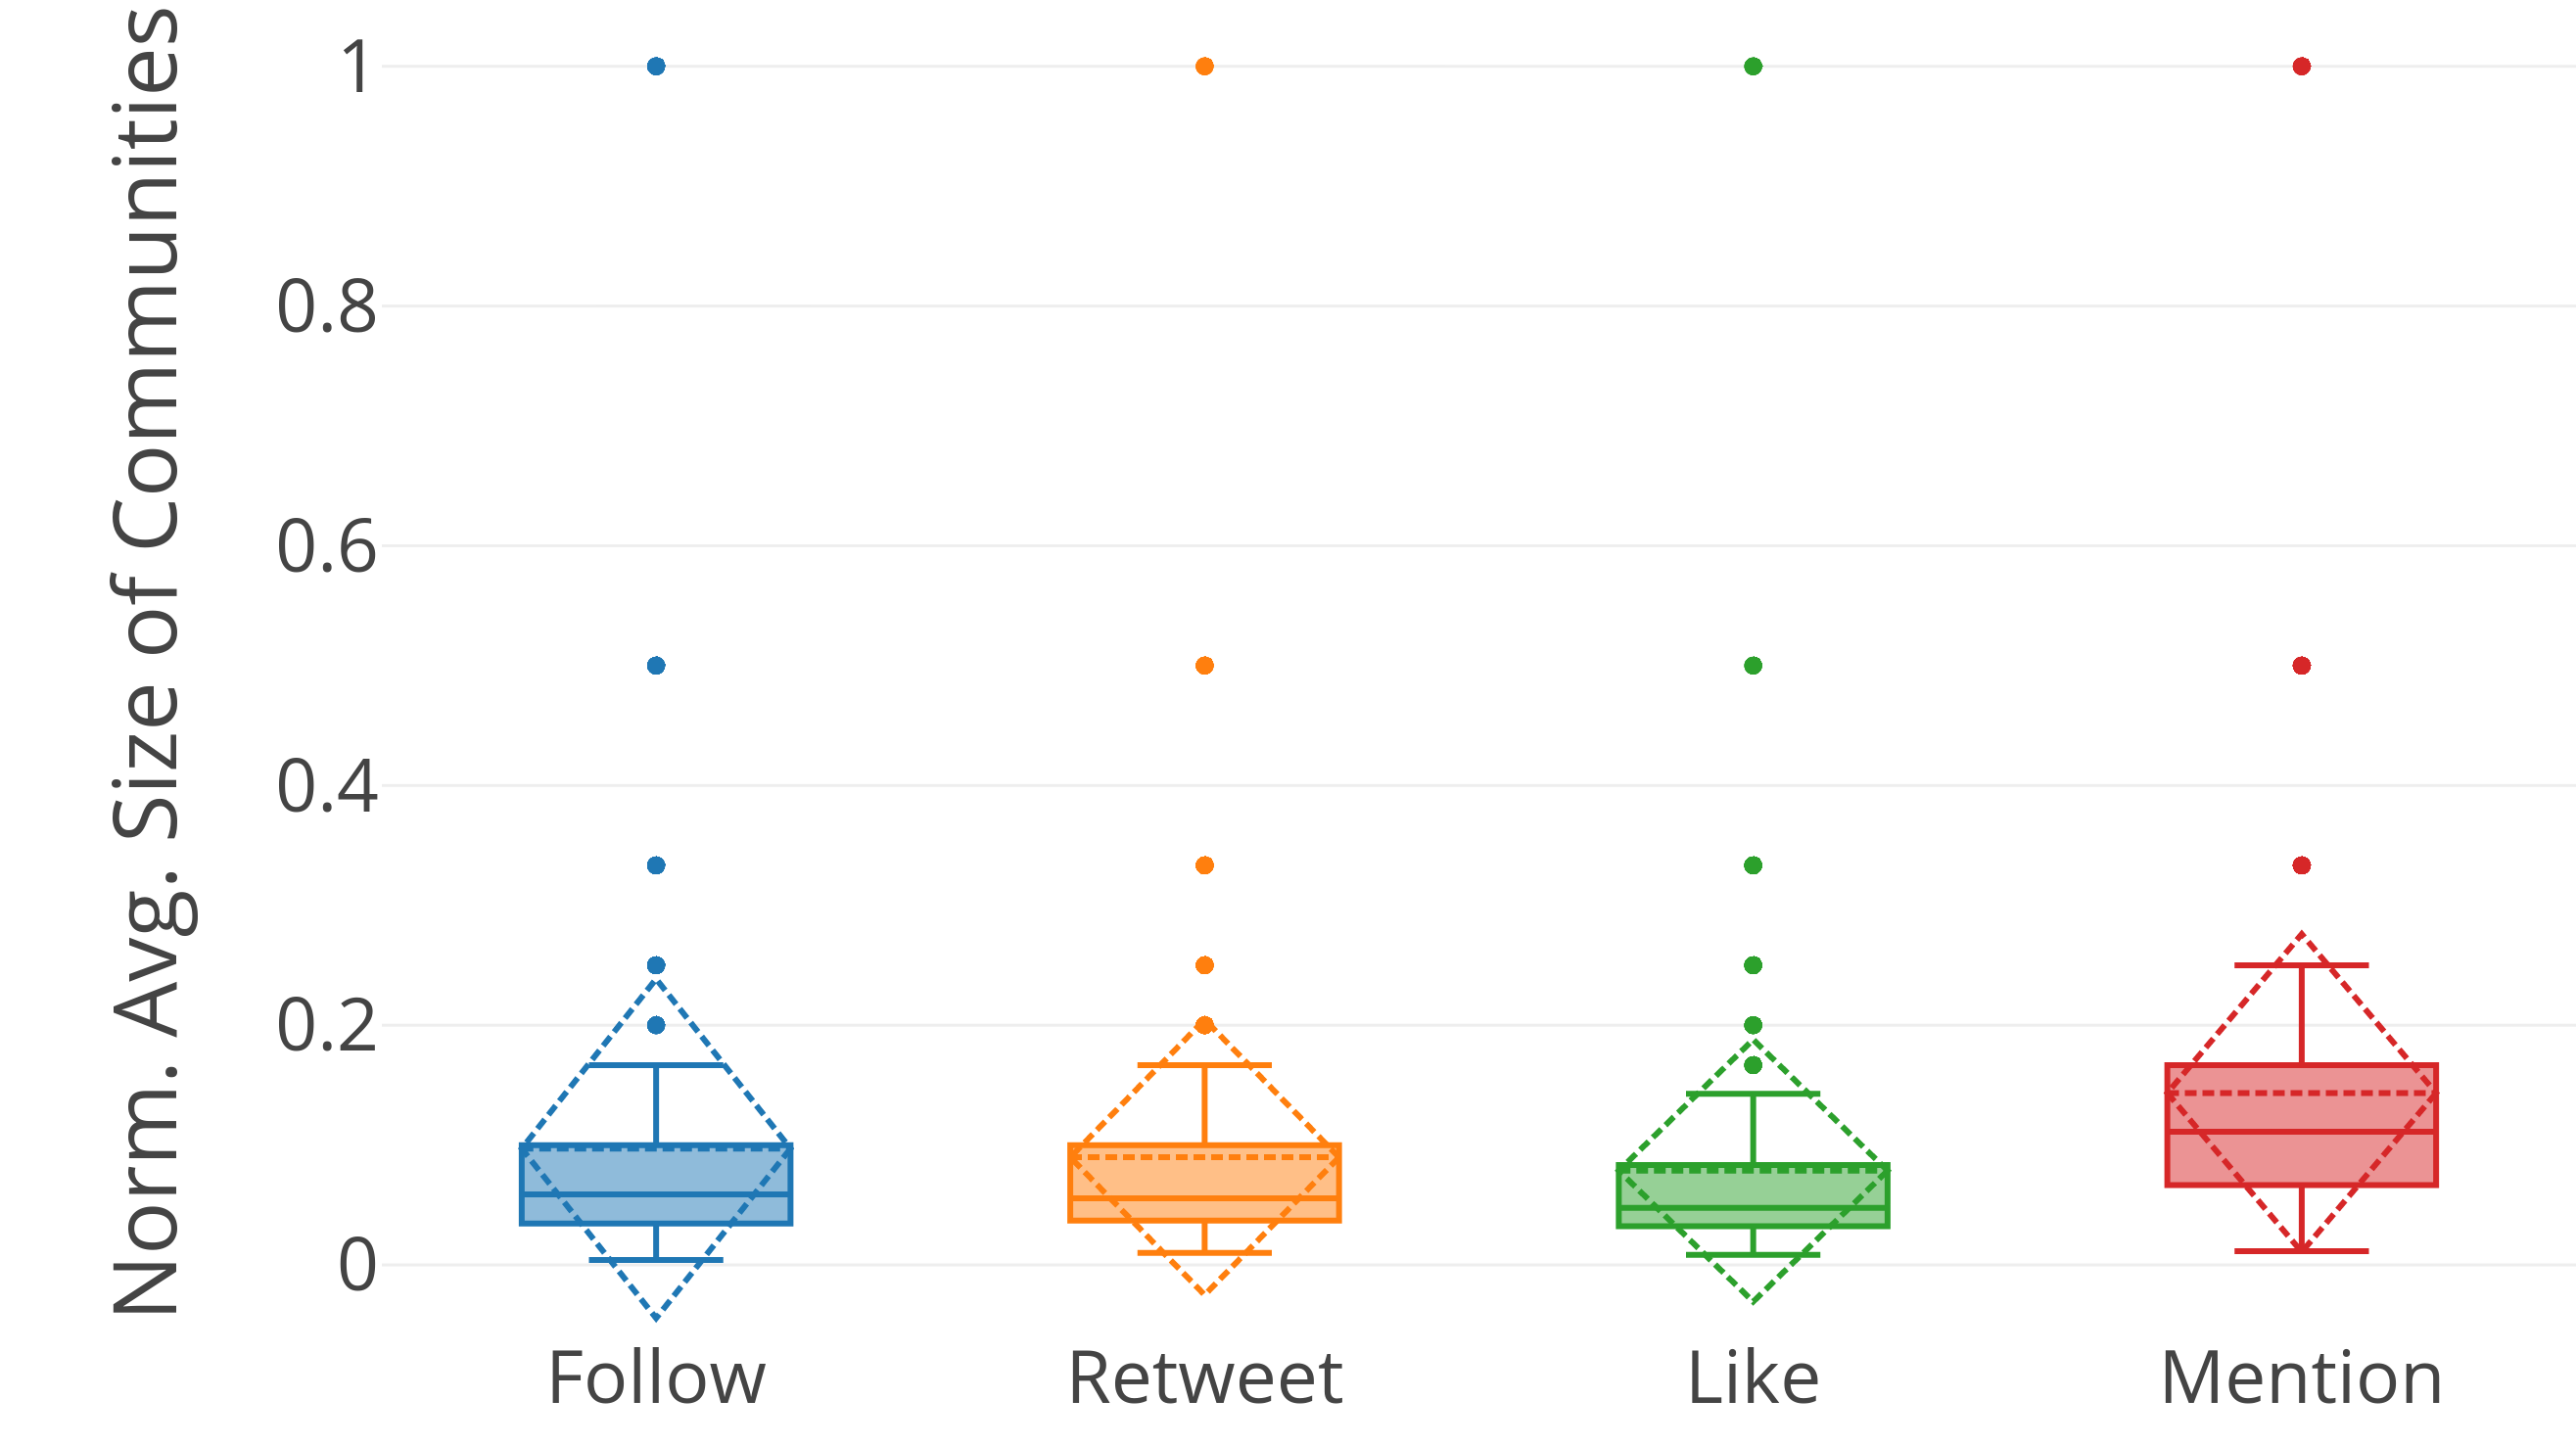
\includegraphics[width=0.47\textwidth]{fig/comm_stats/infomap/comm_stats_norm_avg_comm_infomap.png}
        \label{fig:comm_stats_avg_size_comm_infomap}
    } \\
    \subfigure[COPRA]{
        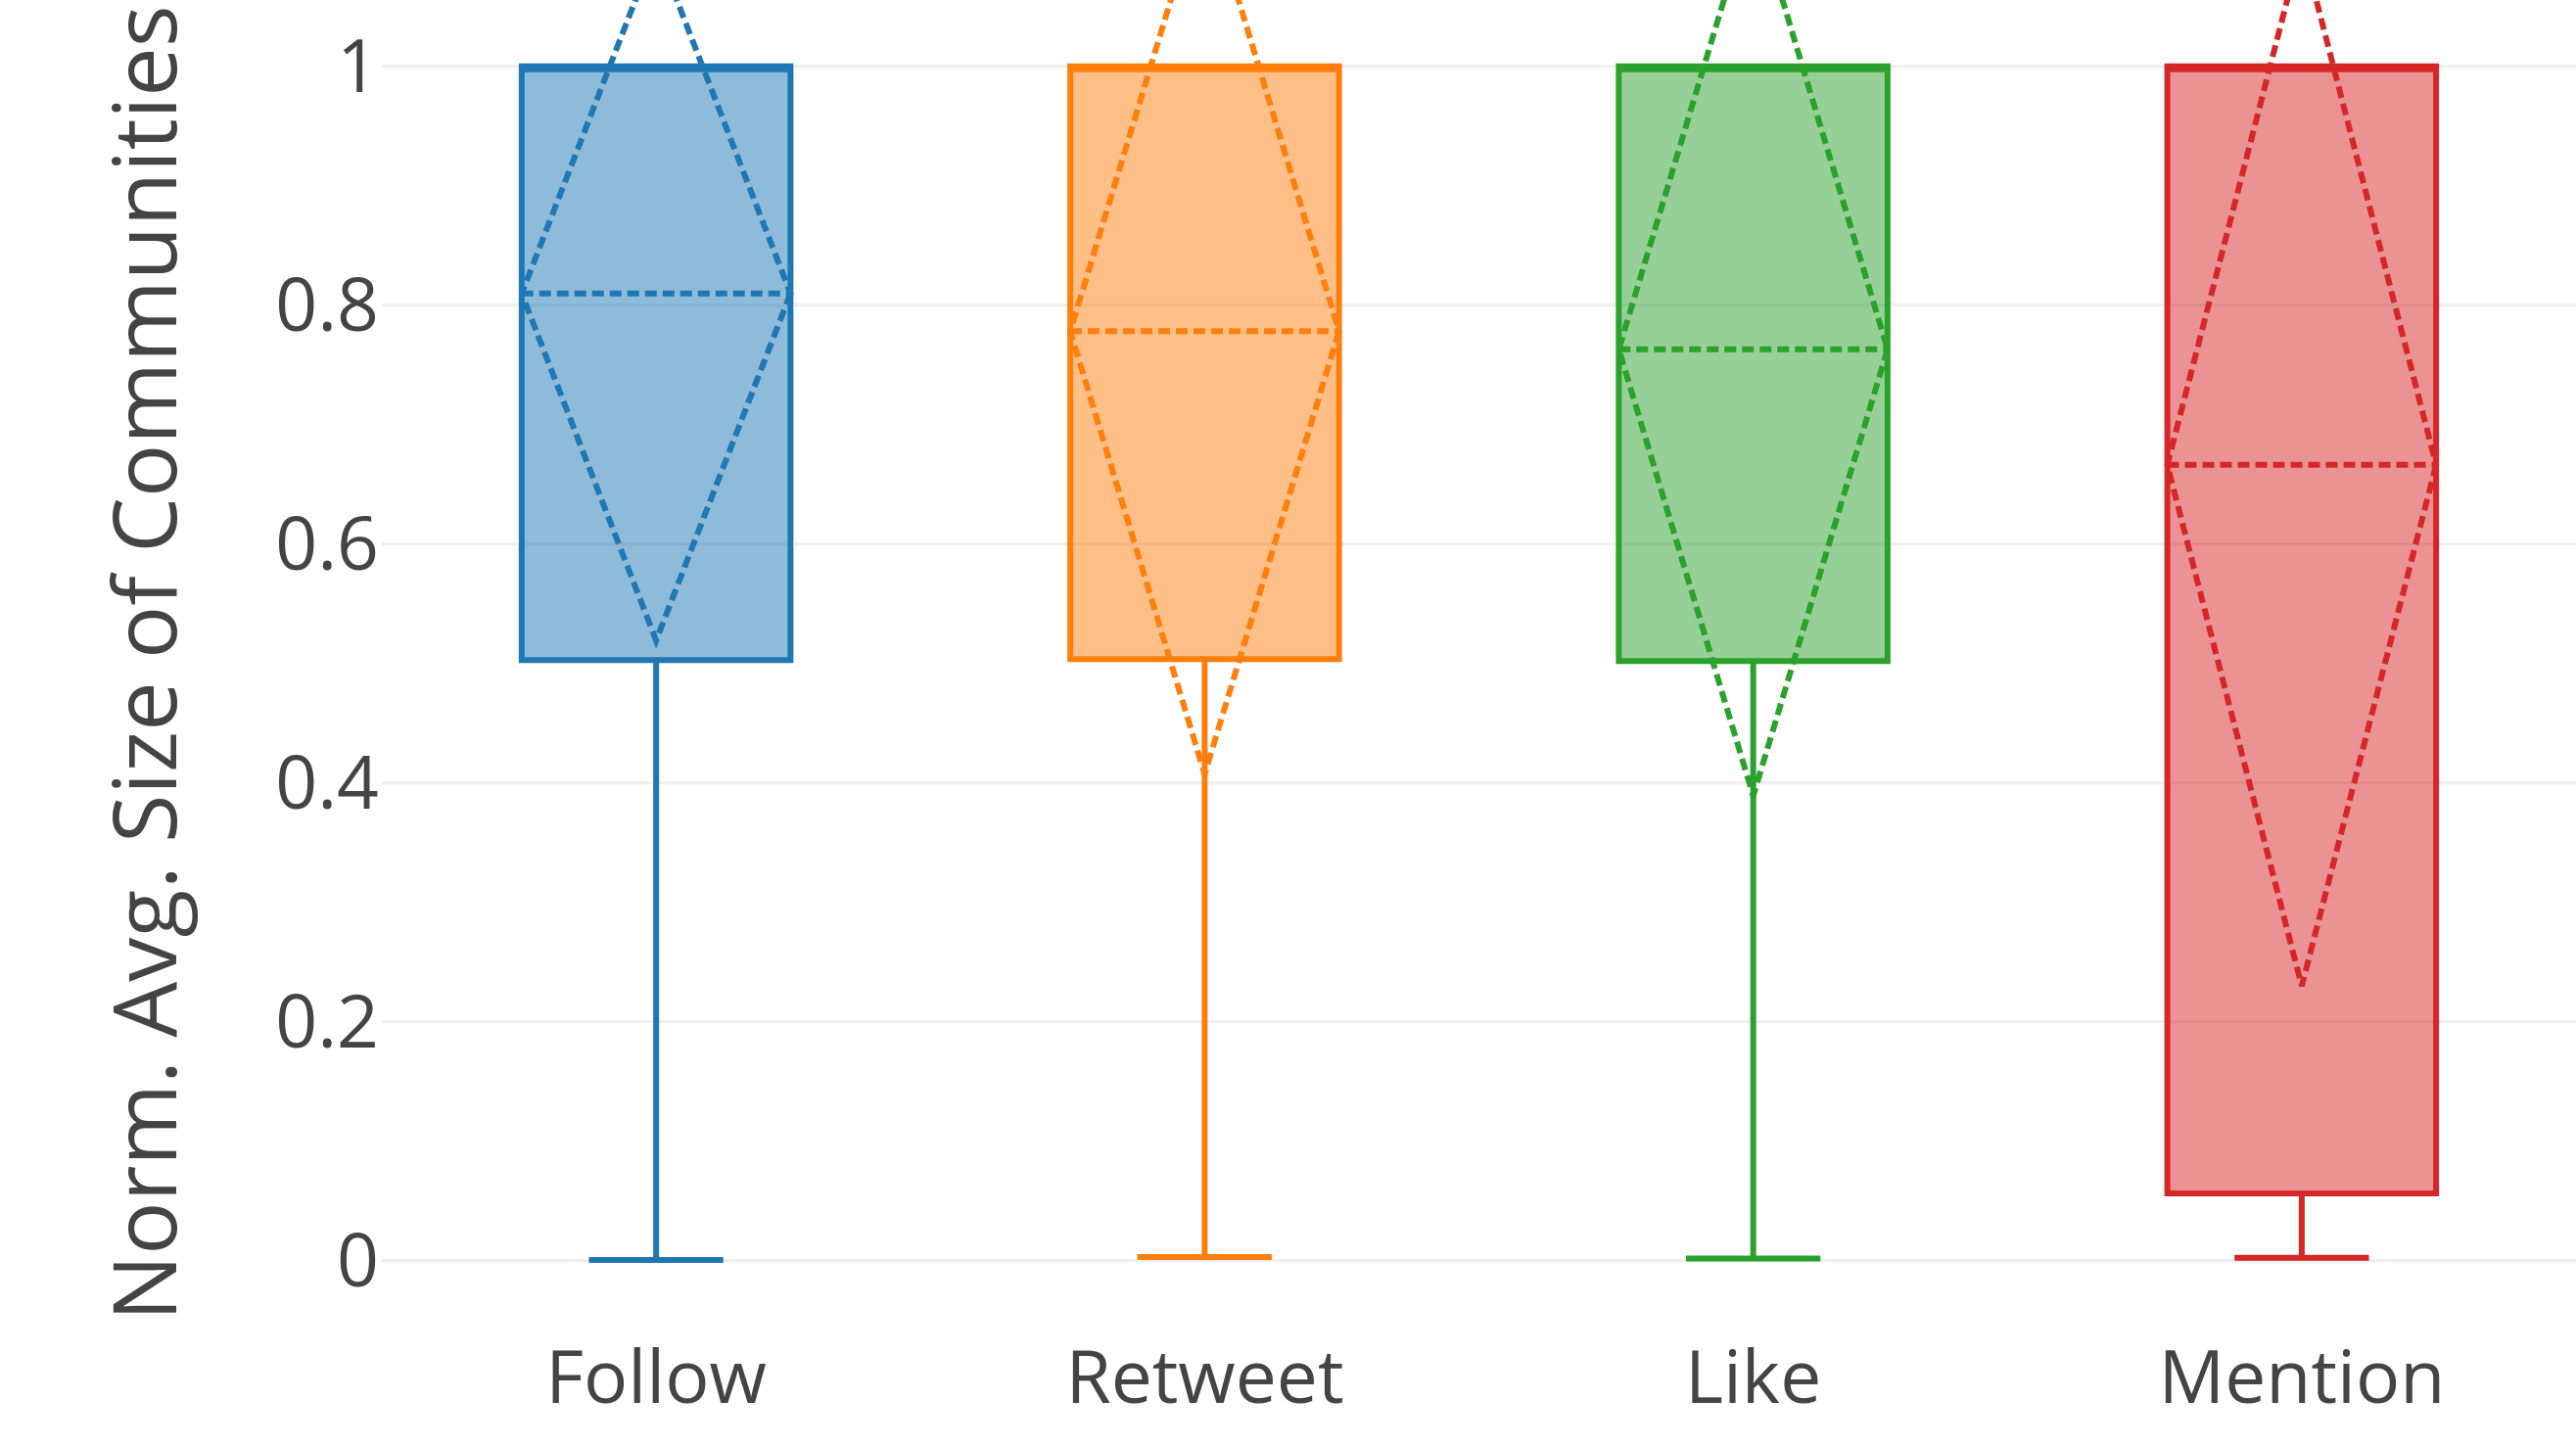
\includegraphics[width=0.47\textwidth]{fig/comm_stats/copra/comm_stats_norm_avg_comm_copra.png}
        \label{fig:comm_stats_avg_size_comm_copra}
    }
    \subfigure[OSLOM]{
        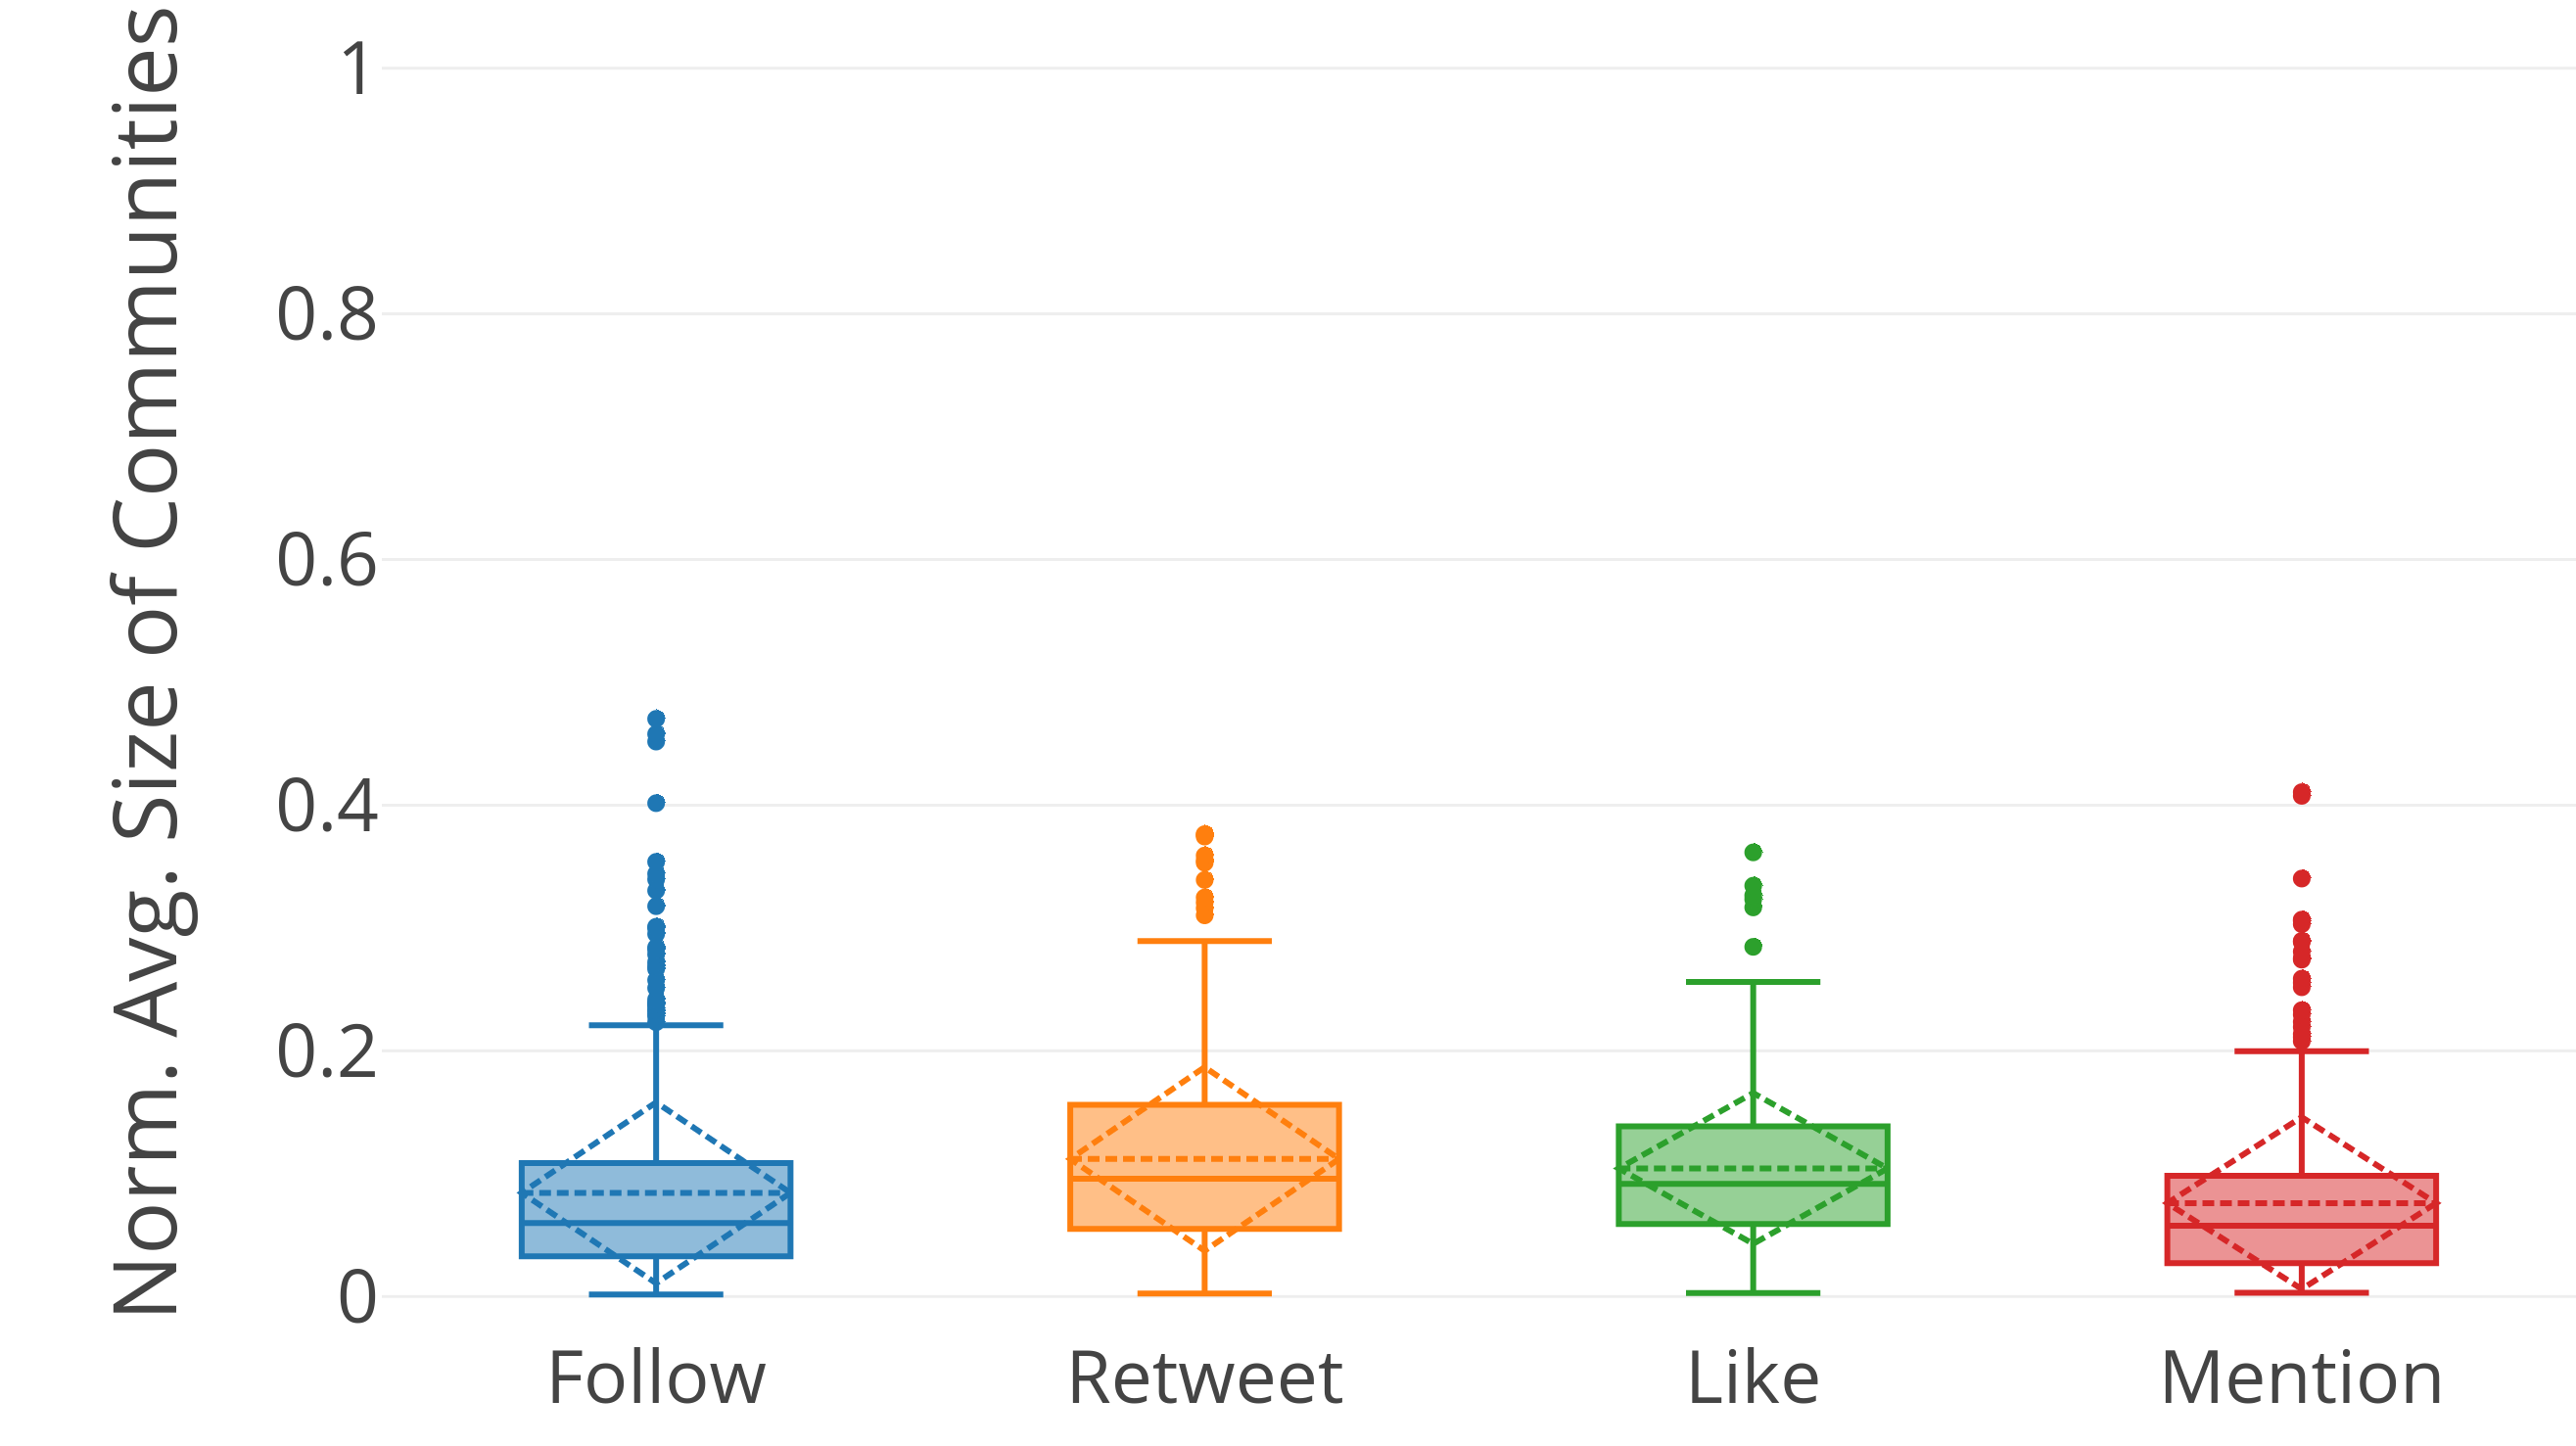
\includegraphics[width=0.47\textwidth]{fig/comm_stats/oslom/comm_stats_norm_avg_comm_oslom.png}
        \label{fig:comm_stats_avg_size_comm_oslom}
    }
    \caption{Average size of communities detected in each layer normalized by the order of the ego networks.}
    \label{fig:comm_stats_avg_size_comm}
\end{figure}



\begin{figure}[h!tb]
    \centering
    \subfigure[RAK]{
        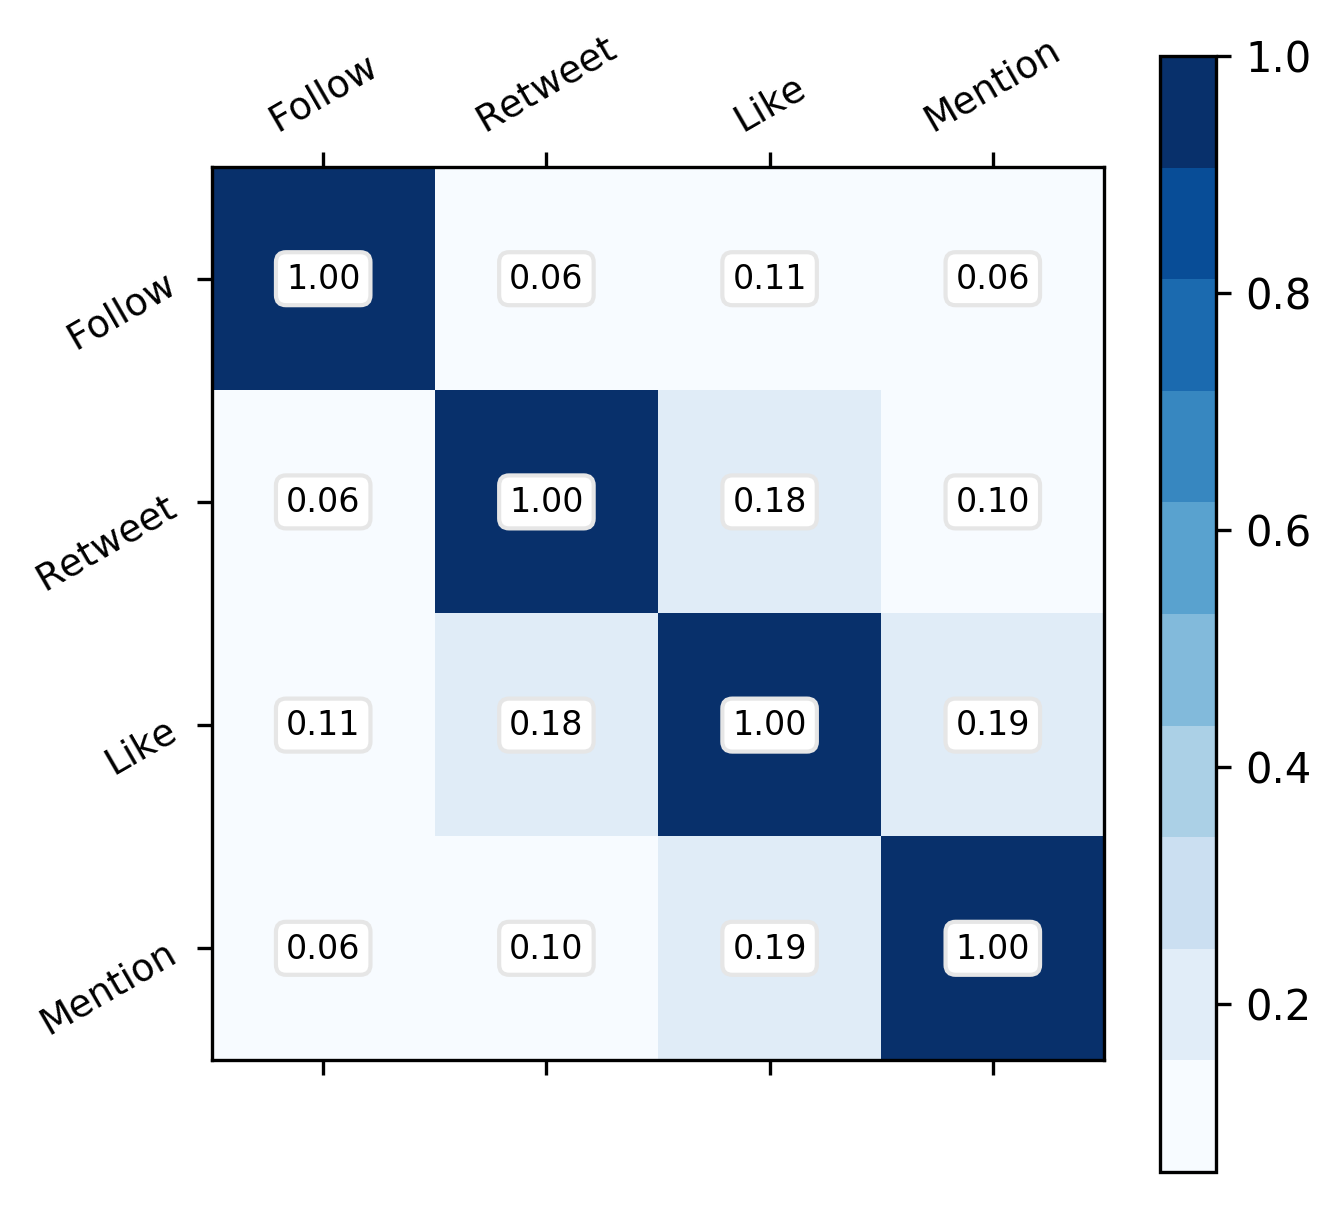
\includegraphics[width=0.47\textwidth]{fig/comm_stats/rak/n_comm_correlation_spearman.png}
        \label{fig:comm_stats_n_comm_correlation_rak}
    }
    \subfigure[INFOMAP]{
        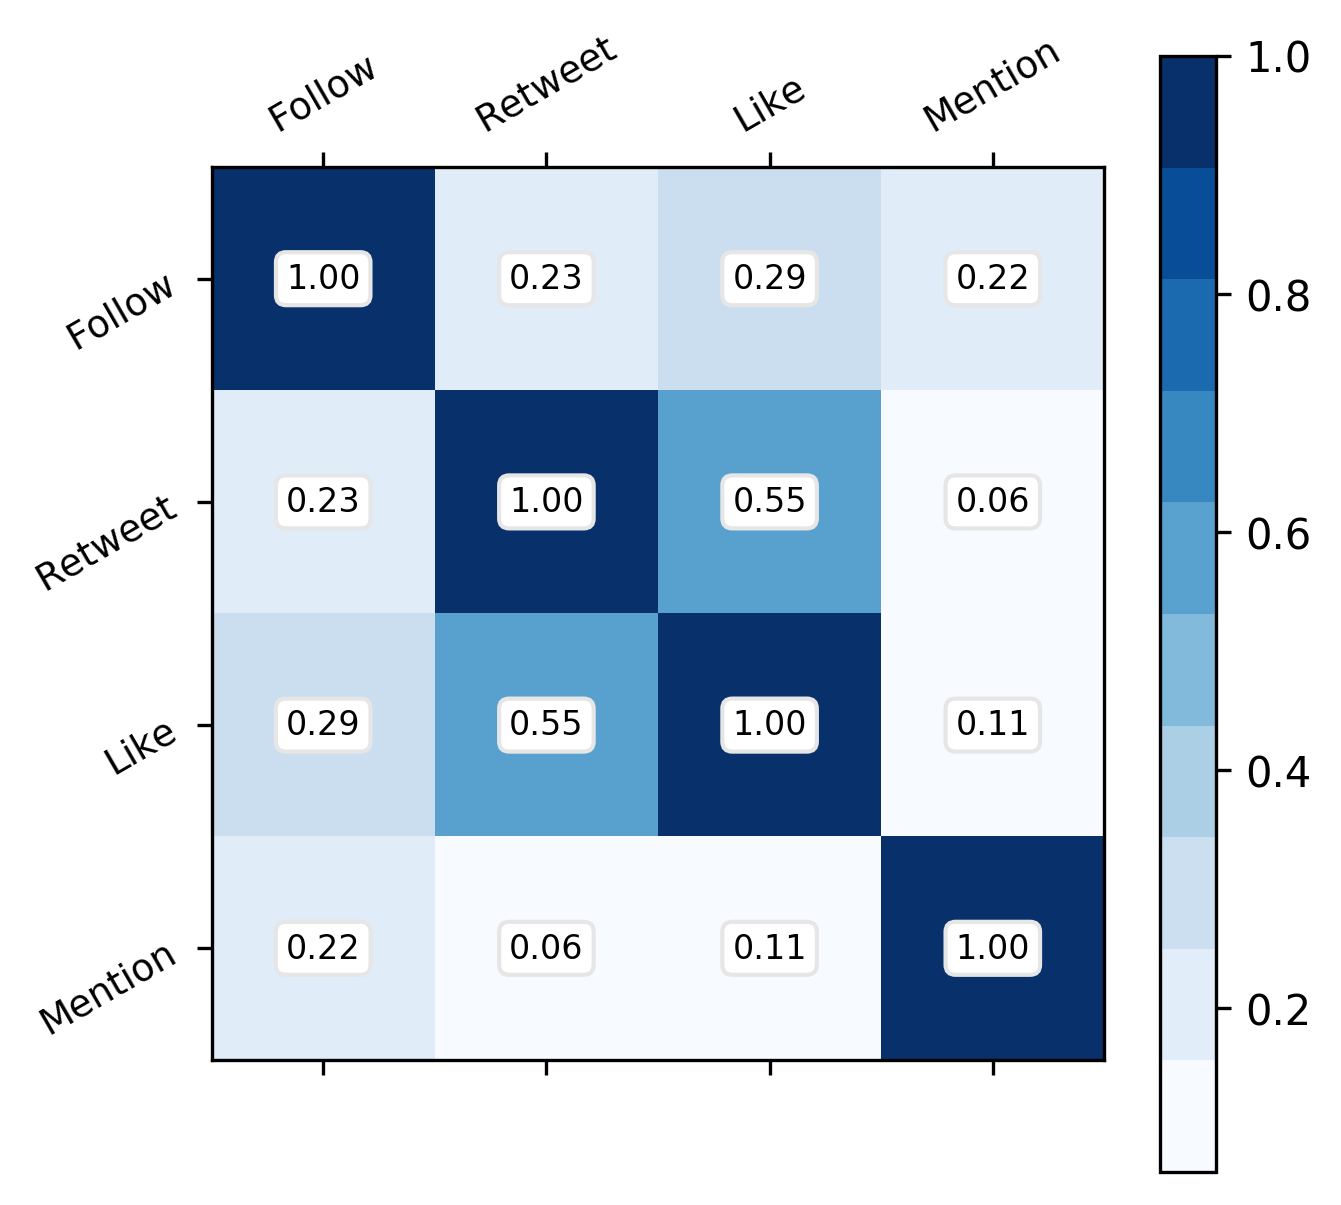
\includegraphics[width=0.47\textwidth]{fig/comm_stats/infomap/n_comm_correlation_spearman.png}
        \label{fig:comm_stats_n_comm_correlation_infomap}
    } \\
    \subfigure[COPRA]{
        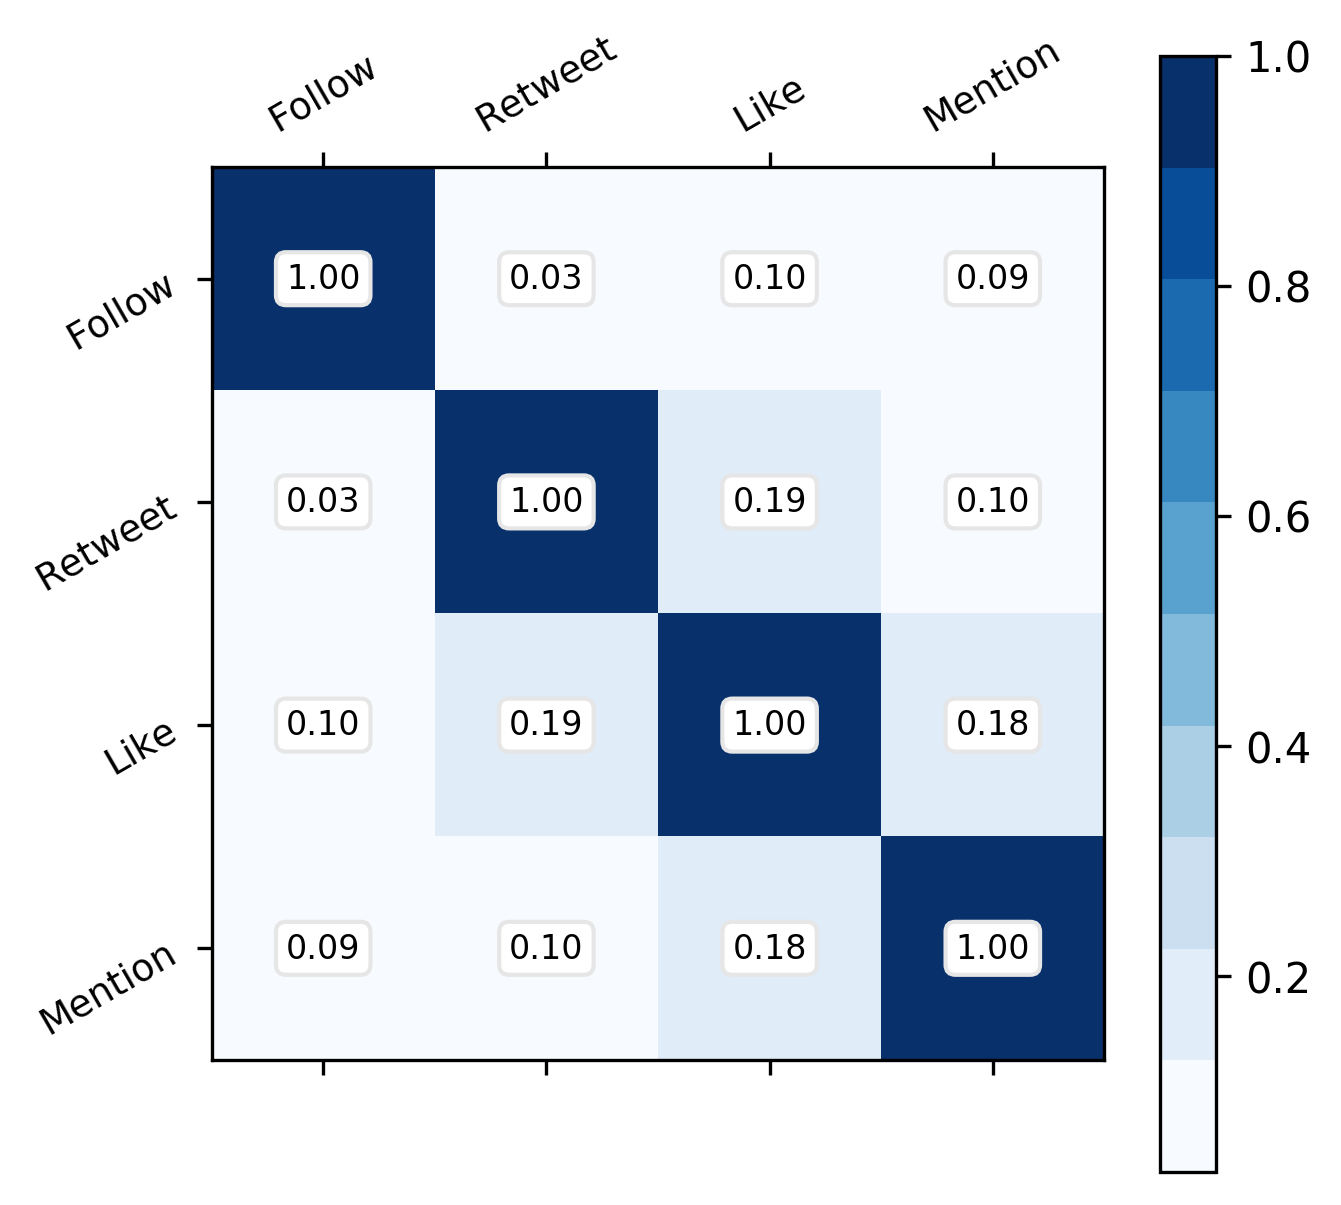
\includegraphics[width=0.47\textwidth]{fig/comm_stats/copra/n_comm_correlation_spearman.png}
        \label{fig:comm_stats_n_comm_correlation_copra}
    }
    \subfigure[OSLOM]{
        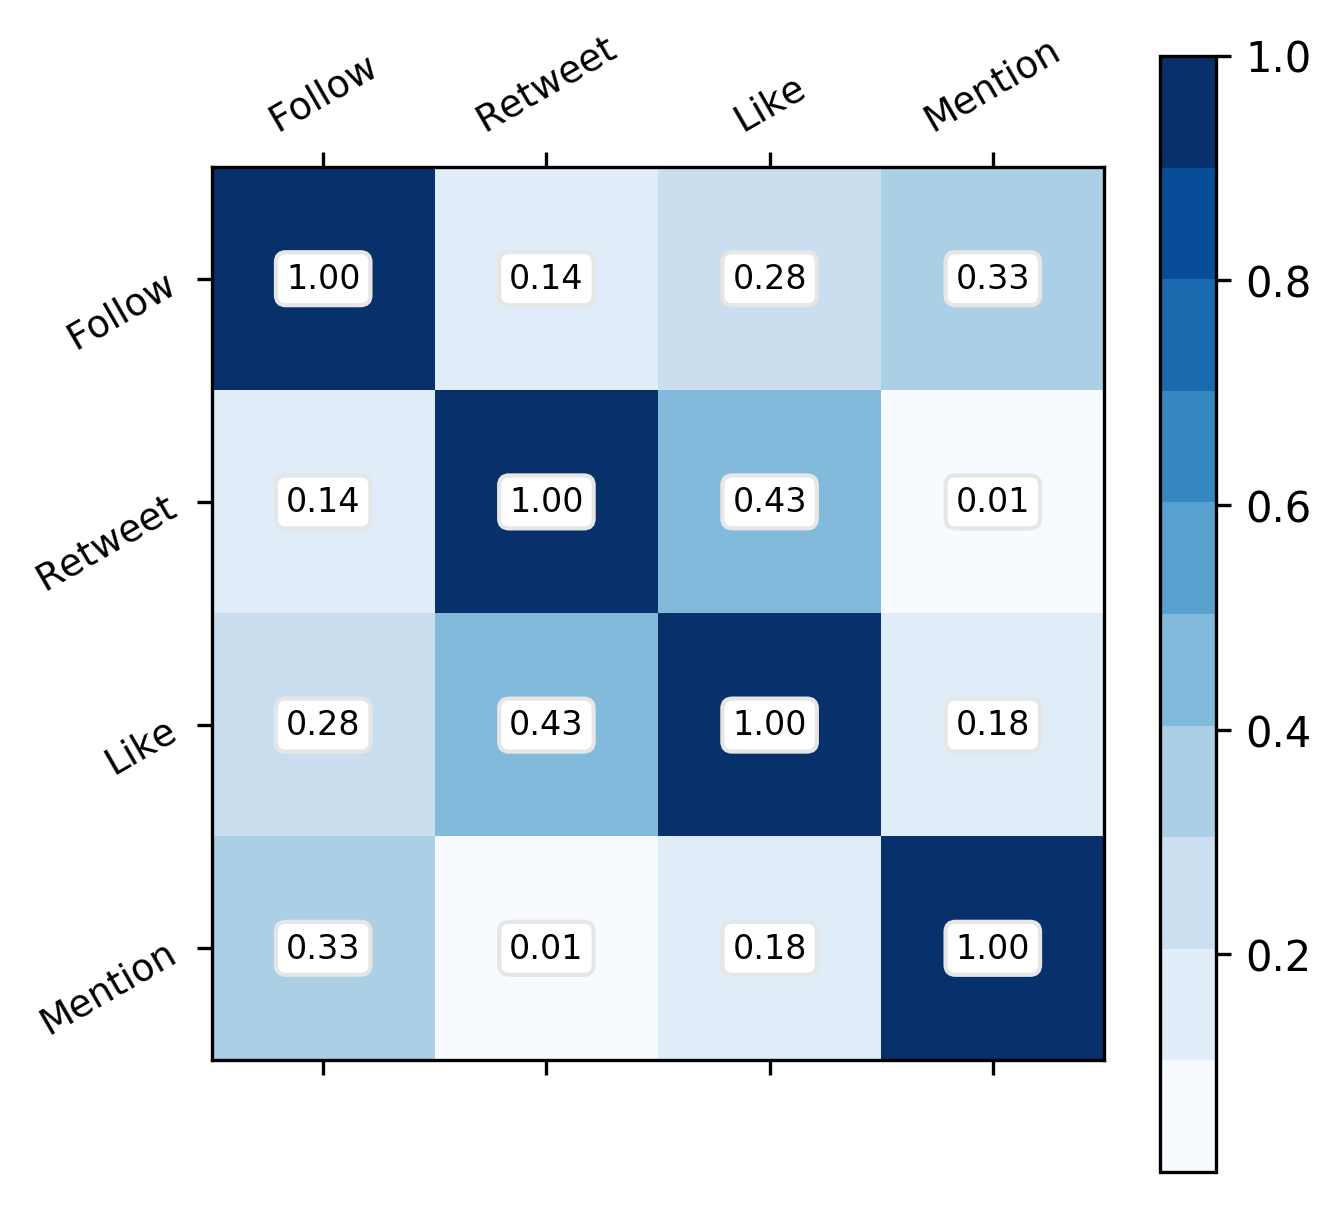
\includegraphics[width=0.47\textwidth]{fig/comm_stats/oslom/n_comm_correlation_spearman.png}
        \label{fig:comm_stats_n_comm_correlation_oslom}
    }
    \caption{Spearman's correlation between the layers for the number of communities detected in each layer.}
    \label{fig:comm_stats_n_comm_correlation}
\end{figure}

Figure \ref{fig:comm_stats_avg_size_comm} displays a boxplot with mean values for the size of the communities found in each ego network. This value is normalized by the size of the ego networks. It is noted that the RAK \ref{fig:comm_stats_avg_size_comm_rak} and COPRA \ref{fig:comm_stats_avg_size_comm_copra} algorithms present the highest values, indicating that, according to these algorithms, for most ego networks there is a very large single community formed by almost all or all of the vertices of the graph, although the mention layer greater variation. As for the algorithms INFOMAP \ref{fig:comm_stats_avg_size_comm_infomap} and OSLOM \ref{fig:comm_stats_avg_size_comm_oslom}, the average community sizes are low, which indicates a larger number of communities detected by these algorithms and, in the case of OSLOM, which detects vertex overlap, communities are also small in relation to the network ego. The interesting thing is that for all the algorithms the results between the layers present little variation.



Figure \ref{fig:comm_stats_n_comm_correlation} shows the Spearman{'}s Correlation between pairs of layers regarding the number of communities detected. We found weak or moderate correlations between most pairs of layers, except for the pair (retweet, like). As happens in many of the previous analysis, this pair also has affinity in relation to the number of communities. However, despite this affinity, as we reported in Section \ref{sec:net_structure}, for many egos these two pair of layers have different set of vertices and different of edges which makes their communities to be also distinct from each other.  

\begin{figure}[h!tb]
    \centering
    \subfigure[RAK]{
        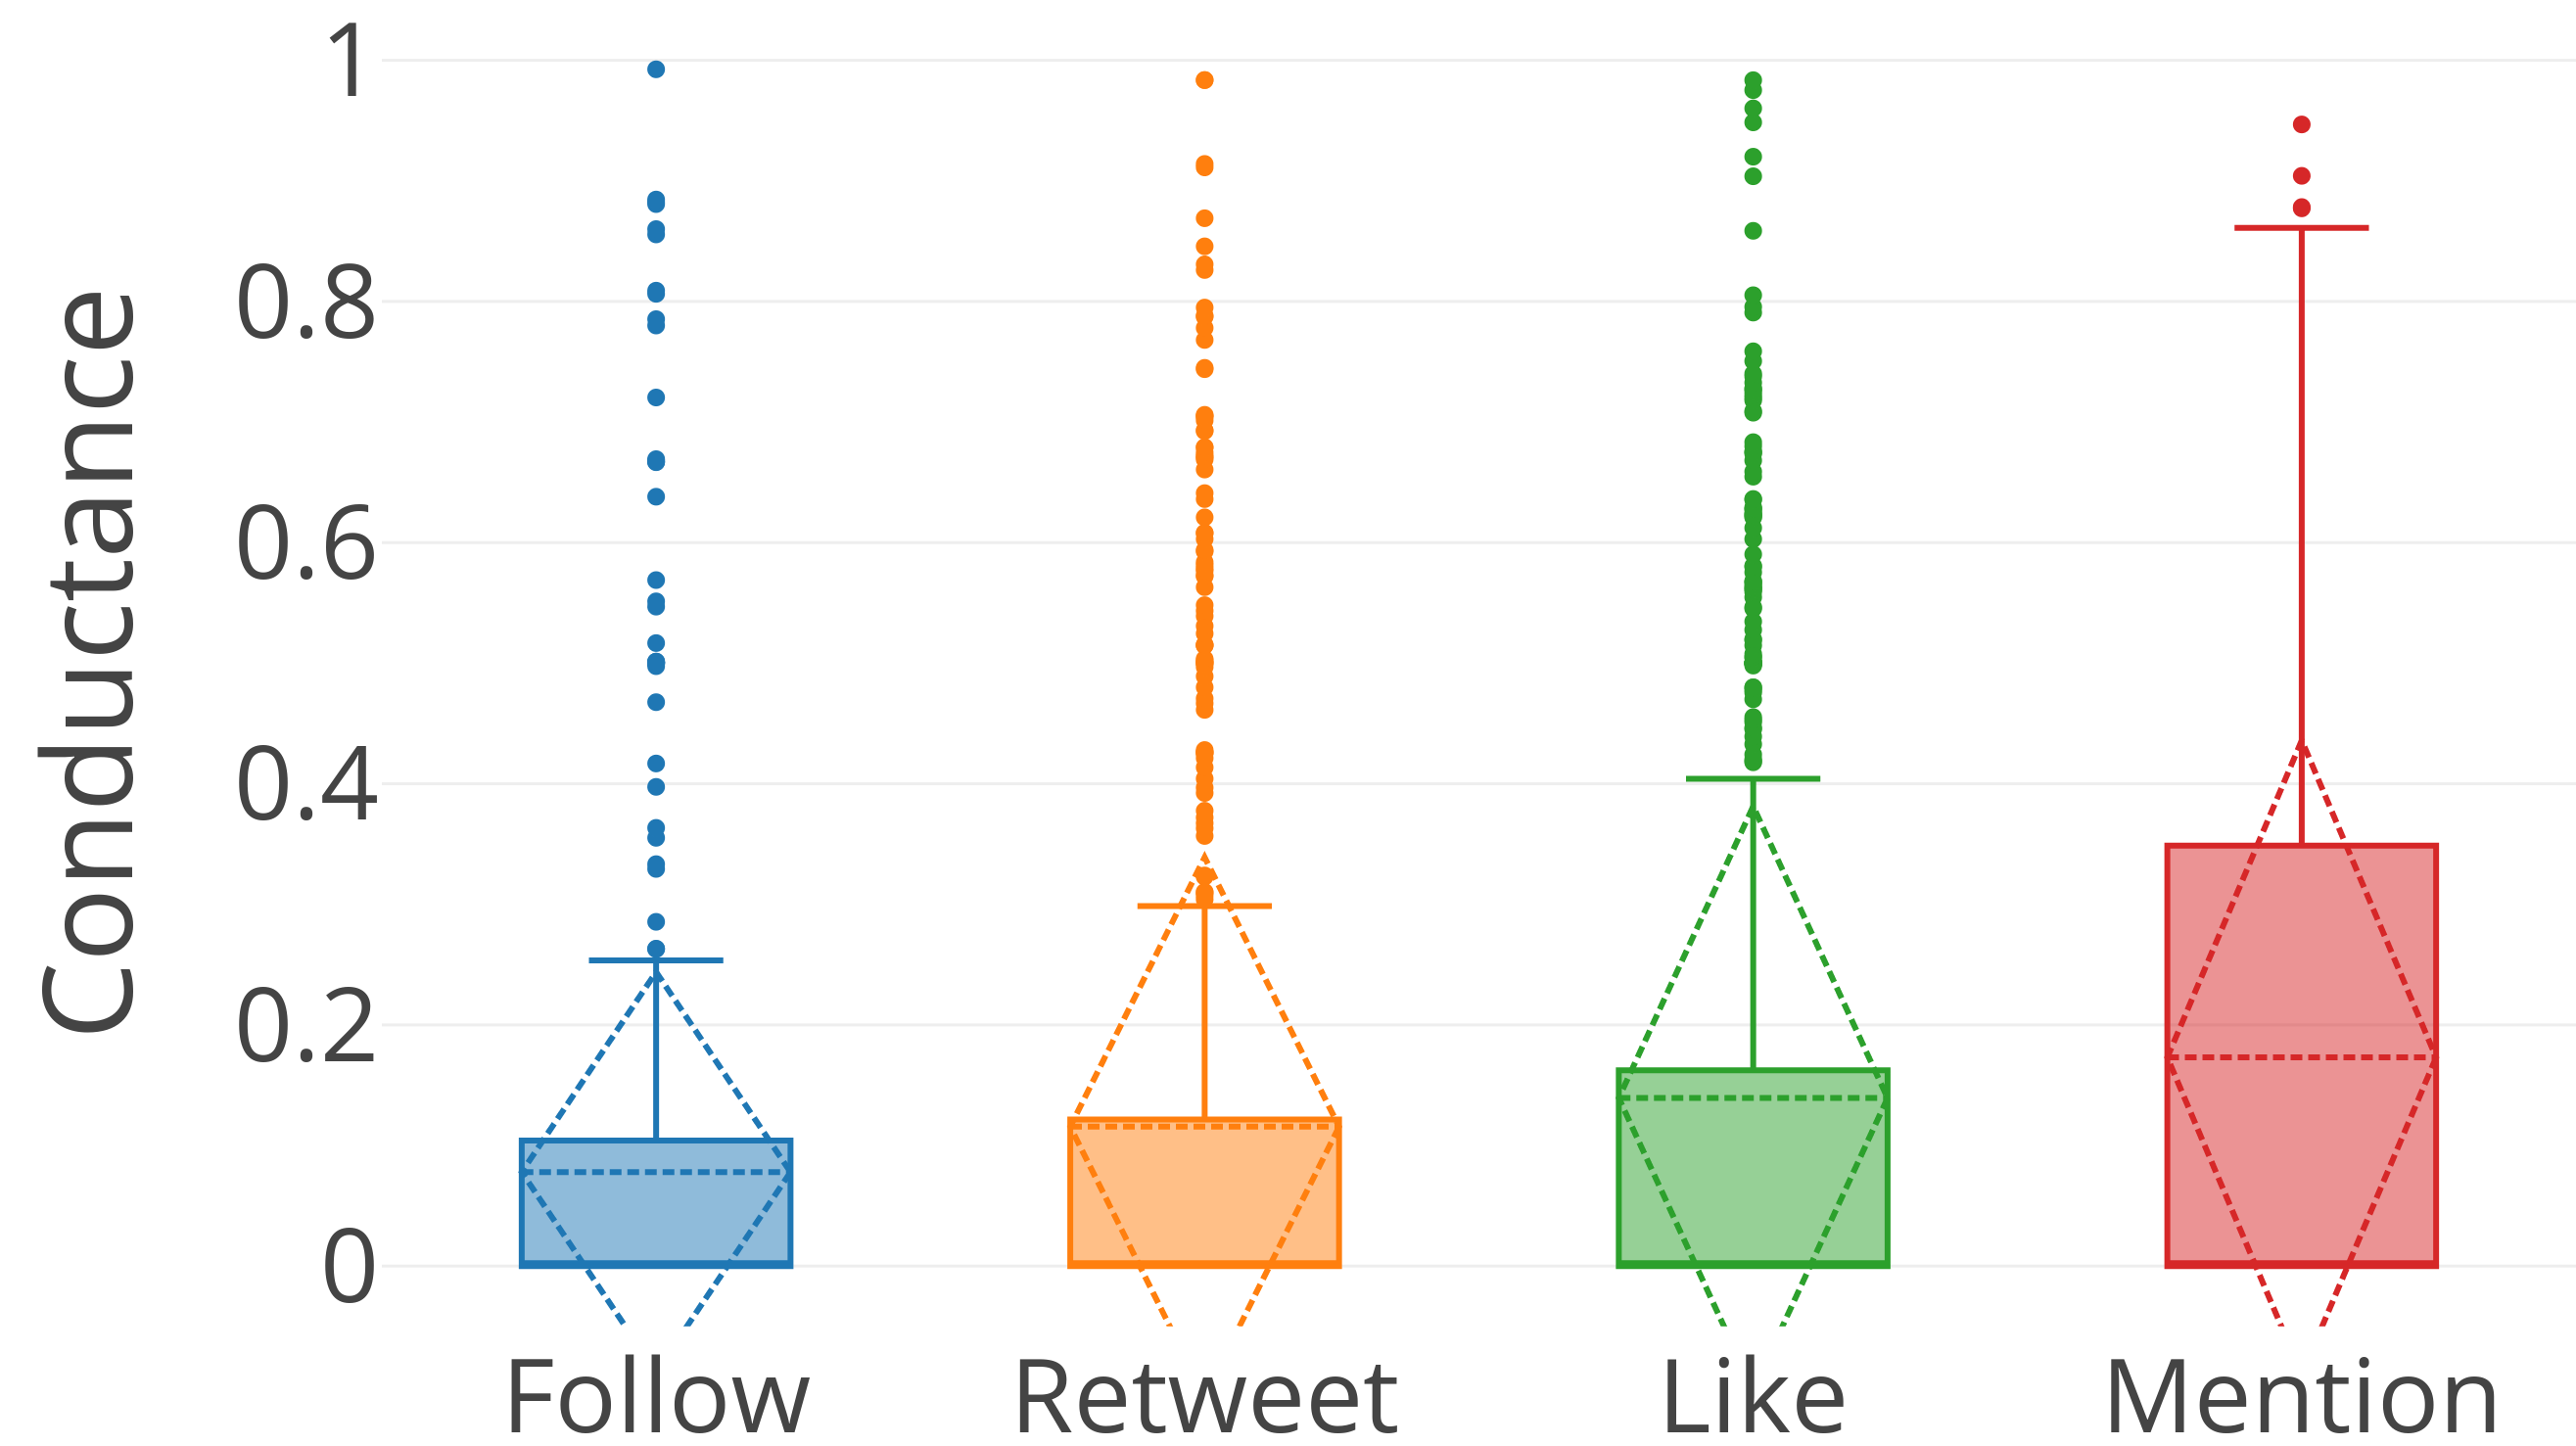
\includegraphics[width=0.47\textwidth]{fig/comm_metrics/rak/rak_conductance.png}
        \label{fig:comm_metrics_conductance_rak}
    }
    \subfigure[INFOMAP]{
        \includegraphics[width=0.47\textwidth]{fig/comm_metrics/infomap/infomap_conductance.png}
        \label{fig:comm_metrics_conductance_infomap}
    } \\
    \subfigure[COPRA]{
        \includegraphics[width=0.47\textwidth]{fig/comm_metrics/copra/copra_conductance.png}
        \label{fig:comm_metrics_conductance_copra}
    }
    \subfigure[OSLOM]{
        \includegraphics[width=0.47\textwidth]{fig/comm_metrics/oslom/oslom_conductance.png}
        \label{fig:comm_metrics_conductance_oslom}
    }
    \caption{Average Conductance values found in detected communities in each layer of the 500 multilayer ego networks.}
    \label{fig:comm_metrics_conductance}
\end{figure}

In order to compare the quality of communities in different layers, we evaluated the communities obtained for each ego and layer using the quality measures described in Section \ref{sec:comm_quality}. The objective of this analysis is to verify if there are significant differences as to the quality of the communities detected in each of the analyzed layers for each mulitplex ego networks, that is, is it possible that one layer produces communities with higher quality than another?



Fig. \ref{fig:comm_metrics_conductance} shows the results obtained from the calculation of the mean conductance of the communities detected by each algorithm in each ego network, according to Eq. \ref{eq:conductance}. The results show that the RAK \ref{fig:comm_metrics_conductance_rak} and COPRA \ref{fig:comm_metrics_conductance_copra} algorithms have the lowest values, which can be explained by the fact that most ego networks have a low number of communities, as shown in Fig. \ref{fig:comm_stats_avg_size_comm}. The OSLOM \ref{fig:comm_metrics_conductance_oslom} algorithm returned communities with very high conductance, indicating that communities are not isolated from each other, with many inter-community edges linking them. The algorithm INFOMAP \ref{fig:comm_metrics_conductance_infomap} brought communities with intermediate values of conductance to the communities. It may be noted that there is little difference when comparing the layers, with the mention layer having a small advantage if we consider a greater number of communities per ego network and that a good community must have low values of conductance.

\begin{figure}[h!tb]
    \centering
    \subfigure[RAK]{
        \includegraphics[width=0.47\textwidth]{fig/comm_metrics/rak/rak_intra_density.png}
        \label{fig:comm_metrics_intra_density_rak}
    }
    \subfigure[INFOMAP]{
        \includegraphics[width=0.47\textwidth]{fig/comm_metrics/infomap/infomap_intra_density.png}
        \label{fig:comm_metrics_intra_density_infomap}
    } \\
    \subfigure[COPRA]{
        \includegraphics[width=0.47\textwidth]{fig/comm_metrics/copra/copra_intra_density.png}
        \label{fig:comm_metrics_intra_density_copra}
    }
    \subfigure[OSLOM]{
        \includegraphics[width=0.47\textwidth]{fig/comm_metrics/oslom/oslom_intra_density.png}
        \label{fig:comm_metrics_intra_density_oslom}
    }
    \caption{Average Internal Density values found in detected communities in each layer of the 500 multilayer ego networks.}
    \label{fig:comm_metrics_intra_density}
\end{figure}


\begin{figure}[h!tb]
    \centering
    \subfigure[RAK]{       \includegraphics[width=0.47\textwidth]{fig/comm_metrics/rak/rak_modularity.png}        \label{fig:comm_metrics_modularity_rak}
    }
    \subfigure[INFOMAP]{
        \includegraphics[width=0.47\textwidth]{fig/comm_metrics/infomap/infomap_modularity.png}
        \label{fig:comm_metrics_modularity_infomap}
    } \\
    \subfigure[COPRA]{
        \includegraphics[width=0.47\textwidth]{fig/comm_metrics/copra/copra_modularity.png}
        \label{fig:comm_metrics_modularity_copra}
    }
    \subfigure[OSLOM]{
        \includegraphics[width=0.47\textwidth]{fig/comm_metrics/oslom/oslom_modularity.png}
        \label{fig:comm_metrics_modularity_oslom}
    }
    \caption{Average Newman{'}s Modularity values found in detected communities in each layer of the 500 multilayer ego networks.}
    \label{fig:comm_metrics_modularity}
\end{figure}

The Internal density of each community was also calculated, according to Eq. \ref{eq:intDensity} and the mean for each of the 500 ego networks can be found in Fig. \ref{fig:comm_metrics_intra_density}. When we compare these results of the internal density of communities with the density of the layers, observed in Fig. \ref{fig:net_struct_density} the values presented by the RAK \ref{fig:comm_metrics_intra_density_rak} and COPRA \ref{fig:comm_metrics_intra_density_copra} algorithms are practically the same found for the density of the entire layer, which reinforces the conclusion that these algorithms detected few or only a community composed of almost all vertices of the ego network. For the INFOMAP \ref{fig:comm_metrics_intra_density_infomap} and OSLOM \ref{fig:comm_metrics_intra_density_oslom} algorithms, the density of the detected communities is much higher than the whole layer density (about one order of magnitude), showing  that all the layers considered show relevant community structure.


The values of Newman's Modularity are shown in Fig. \ref{fig:comm_metrics_modularity}. The calculation of this metric was performed according to Eq. \ref{eq:newmanModularity}. The presentation of the results follows the same procedure adopted for conductance and internal density. The quality of the communities detected by the INFOMAP algorithm is greater than the communities detected by the other algorithms, according to Newman's modularity, as we can see in Fig. \ref{fig:comm_metrics_modularity_infomap} . Again it is not possible to say that one layer stands out from the others. All results fall into the same range of values for all algorithms.

\begin{figure}[h!tb]
    \centering
    \subfigure[RAK]{
        \includegraphics[width=0.47\textwidth]{fig/comm_metrics/rak/rak_mod_density.png}
        \label{fig:comm_metrics_mod_density_rak}
    }
    \subfigure[INFOMAP]{
        \includegraphics[width=0.47\textwidth]{fig/comm_metrics/infomap/infomap_mod_density.png}
        \label{fig:comm_metrics_mod_density_infomap}
    } \\
    \subfigure[COPRA]{
        \includegraphics[width=0.47\textwidth]{fig/comm_metrics/copra/copra_mod_density.png}
        \label{fig:comm_metrics_mod_density_copra}
    }
    \subfigure[OSLOM]{
        \includegraphics[width=0.47\textwidth]{fig/comm_metrics/oslom/oslom_mod_density.png}
        \label{fig:comm_metrics_mod_density_oslom}
    }
    \caption{Average Modularity-Density values found in detected communities in each layer of the 500 multilayer ego networks.}
    \label{fig:comm_metrics_mod_density}
\end{figure}


We also calculate the Modularity-Density according to Eq. \ref{eq:modDensity}, and the result is shown in Fig. \ref{fig:comm_metrics_mod_density}, where the mean Modularity-Density values are displayed for each ego network with a boxplot for each layer. The OSLOM algorithm presents the worst performance for this metric, as we can see in Fig. \ref{fig:comm_metrics_mod_density_oslom}, while the other algorithms show close values for all layers, with the exception of some outliers. The comparison between the layers with the communities detected in the same algorithm also shows that there are no significant differences between them, except for the communities detected by the OSLOM algorithm in the Mention layer, which exhibit the worst results for Modularity-Density.

From the analysis made on the detected communities we can conclude that the distribution of values of all measures are surprisingly very similar for all layers. This information suggests that  the retweet, like, and mention layers have the same potentiality to be used for community detection in ego networks in Twitter as has the follow layer. This is interesting as research opportunity, since in most work related to community detection in Twitter only the graph formed by the following relation is used to determine communities\footnote{In fact, we do not know of any work in literature that uses a graph which edges represent retweets, likes or mentions as the graph used to detect communities.}. We think that investigating community detection in the other three layers may be potentially interesting for the following reasons:
\begin{itemize}
    \item This interactions are directly related to tweets and, consequently, to the topics included in them. Thus, it it is possible that communities detected in these layers  be more topic-related than communities detected in the follow graph, since the follow relation is not directly related to informations transmitted in tweets.
    \item Directed graphs based on retweets, likes and mentions may naturally be extended to weighted graphs. We can associate a  weight to the edge between two users $a$ and $b$ corresponding to the number of times $a$ interacted with $b$ via a tweet using one of these interactions. For instance, in the case of a retweet graph, the weight of an edge $(a,b)$ represents the number of times $a$ retweeted a tweet authored by $b$. Many  community detection algorithms  can be extended to be applied  to  directed weighted graphs. Communities obtained  in weighted graphs may be more meaningful for  also taking intensity of interactions as additional information in community detection.
\end{itemize}


%%%%%%%%%%%%%%%%%%%%%%%%%%%%%%%%%%%%%%%%%%%%%% 
%%%%%%%%%%%%%%%%%%%%%%%%%%%%%%%%%%%%%%%%%%%%%% 


\section{What is the intersection between egos' lists and her layers?}
\label{sec:QuestionTwitterLists}
A Twitter list is a feature that users have to arbitrarily group other users. The list curation is allowed to all users and carried out manually. The owner of a list - the one who created it - starts receiving the tweets and retweets posted by the list members on a special timeline. A user can subscribe to a list of another user and also receive the tweets and retweets of the members of that list in a separate environment. This feature gives Twitter users the ability to manually enter other users into communities according to the personal criteria of the list owner.

Users who subscribe to the lists agree with the way the owner has organized and inserted the members, so we consider that they are also part of the community because they share a common interest with the owner. Thus, for each ego we calculate some measures to verify if communities formed from their lists can be used as ground truth for the communities detected in each layer of the multilayer ego networks.

\begin{figure}[h!tb]
    \centering
    \includegraphics[width=1\textwidth]{fig/lists_stats/alters_intersection_over_lists_set.png}
    \caption{Percentage of the lists users found in the alter set.}
    \label{fig:lists_alters_over_lists}
\end{figure}

Figure \ref{fig:lists_alters_over_lists} shows the results obtained by calculating the percentage of users associated with the ego lists (members and subscribers) that also appear in the alter set of each layer. There is a very large variation in the results, with the median distant from the mean and the indication that for the great majority of egos the number of users of the lists that appears in the set of alters is below 40\%. The only layer that has higher values is the follow layer, where for 75\% of the ego about 60\% of all users associated with the lists are in the set of vertices. For the other 25\% of the ego of this layer this value varies between 60\% and 100\%.

The above result suggests that lists are used to group the users to whom the ego follows and that there is little interaction between the ego and the list elements. Another relevant information is that even with the follow layer presenting the highest values, there are a considerable number of users who are members or are enrolled in ego lists but who are not ego friends, although the concept of the lists shows that they have an interest in common and therefore would tend to be friends.


\begin{figure}[h!tb]
    \centering
    \includegraphics[width=1\textwidth]{fig/lists_stats/lists_intersection_over_alters_set.png}
    \caption{Percentage of alters that were found in the ego{'}s lists.}
    \label{fig:lists_lists_over_alters}
\end{figure}

We also analyze whether the set of alters can be found in the ego lists. Figure Y shows the result for this calculation. It can be observed that for all layers the values are very low. For 75\% of the egos about 20\% of the alters appear in the lists, this for all strata analyzed. With the information cleared it would be impracticable to use the lists as ground truth for the communities detected in the retweet, like and mention layers, since the set of alter and the set of list elements are very different.

The results of the calculations performed with the elements of the ego lists can be explained by the fact that the feature of the lists may not have been very well accepted and adopted by the users, since the organization of the lists needs to be done manually. In the literature there are already works that seek to group the users and create the lists automatically \cite{Wang2012,Wang2015}, and in these cases maybe the list could be an alternative to the lack of ground truth in Twitter.

The results indicate that even the follow layer presenting the largest intersection between the alters and the list elements there are a considerable number of users who are members or are enrolled in ego lists but who are not ego friends. This shows that Twitter should recommend to the ego the option of following the elements of the lists that it owns or is enrolled. The lists allow the ego to view content published only by its members and not by the subscribers, ie the ego does not view the content published by other users who are on its lists although they have an affinity with the ego because they are interested in content in common.
%\begin{figure}[h!tb]
%    \centering
%    \includegraphics[width=1\textwidth]{fig/lists_stats/lists_intersection_over_topk.png}
%    \caption{Percentage of top-k alters that appear on at least one of the ego lists.}
%    \label{fig:lists_topk_over_lists}
%\end{figure}

%1) How the sizes of the ego networks vary among layers in terms of both number of vertices and number of edges? Is there correlation beteween the sizes of the layers related to the same ego?
%
%2) As camadas das redes egos são de escala livre (free scale)? 


%%%%%%%%%%%%%%%%%%%%%%%%%%%%%%%%%%%%%%%%%%%%%%%%%
%Há correlação entre o tamanho da rede (número de alters) e o fato de ela ser scale-free? 
%%%%%%%%%%%%%%%%%%%%%%%%%%%%%%%%%%%%%%%%%%%%%%%%%

%
%
%3) As redes egos de cada  camada formam um small world?
%
%4) Qual a similaridade entre as diversas camadas de rede ego ?
%
%4.1)  Os  elementos de maior grau de uma camada ocorrem nas demais camadas?
%
%5) As camadas das redes egos tendem a formar comunidades?
%%%%%%%%%%%%%%%%%%%%%%%%%%%%%%%%%%%%%%%%%%%%%%%%%
%5.1 Existe correlação entre o tamanho das redes e o número de comunidades?
%5.2 Existe uma grande comunidade? 
%%%%%%%%%%%%%%%%%%%%%%%%%%%%%%%%%%%%%%%%%%%%%%%%%

%5.3 Qual a qualidade das comunidades formadas?
%5.4 As listas servem de ground truth para as comunidades nas camadas? 
\chapter{Final Considerations}
\label{cap:Considerations}

This work presented the conduction of an extensive structural analysis of 500 ego networks multilayers of Twitter. From the modeling of four layers representing the types of {\em follow, retweet, like} and {\em mention} interactions, it was possible to identify and characterize the main structural properties of these networks. To the best of our knowledge a detailed study of layers composing the network of a user in Twitter has not been reported until now. 

Next, in Section \ref{sec:conclusion}, is the conclusion of the work with the description of the main results found and on how they can contribute to the advancement of research on the subject here discussed; and in Section \ref{sec:future} are listed some of the next steps that can be given from the knowledge acquired with this dissertation, or the fact that some questions still lack further research to achieve satisfactory results.


%%%%%%%%%%%%%%%%%%%%%%%%%%%%%%%%%%%%%%%%%%%%%% 
%%%%%%%%%%%%%%%%%%%%%%%%%%%%%%%%%%%%%%%%%%%%%% 


\section{Conclusion}
\label{sec:conclusion}

The objectives proposed for this work were reached. A structural analysis of the multilayer ego networks was performed on Twitter and we addressed several issues with regard to the layers of Twitter ego networks. First,  we found that despite  great variations both in the number of vertices and edges in the same layers for different egos, the density in all layers are similarly low. Most  egos do not achieve 10\% of density in any layer. Also, most edges are not ego-alter edges,  meaning that there is many interaction between alters in a layer.

 
%the  mean clustering coefficients of layers are greater than a corresponding random graph. The mean average shortest path lengths of the layers are, on the contrary, very similar to ones found in the corresponding random graphs. These characteristics allowed us to conclude that the great 
%. 

We also found that the majority of layers of all egos are small worlds, an interesting property regarding the flow of communication in these layers. The layers are also scale-free for most egos, when regarding indegree distribution. 
%This means that in every layer there is a small group of important vertices which receive many interactions from many other vertices and the great majority of vertices receiving very few interactions. 
 
The high clustering coefficient of vertices  in each layer leads to formation of community sets  with the following characteristics: a) the communities are dense subgraphs, with density much superior to that of the whole layer; b) communities in the set are interconnected as demonstrated by the high values of conductance we found; c) the sets are formed by at least one big community and tens of small communities, not achieving 10\% of the size of the biggest one. Besides, these characteristics are very similar in all layers, indicating that all layers have the same potential to form communities.

There is considerable overlap between the alter sets of different layers for an ego, with most egos having at least 30\% of overlap between any pair of layers. This lead us to conclude that there is much opportunity for information diffusion in the ego network, i.e. not only each layer is a small world but these small worlds intercept each other. Besides, we found considerable overlap between hubs (high indegree vertices) between layers, meaning that some nodes are influential regarding more than one type of interaction. 

Also, our analysis  allowed also to find and interesting potential problem caused by misuse of the follow operation by about 25\% of the users of our sample. These users do not follow up to 35\% of the top ten alters they retweet most. This is not  only a problem for the users themselves, but may also affect the propagation of tweets throughout the followers of these users.

Finally we looked at the ability of Twitter lists to serve as ground truth for the problem of detecting communities in Twitter’s ego networks and concluded that this is not feasible. There is little interaction between the ego and the list elements and the intersection of the alters sets of each layer with the list elements is very low, that is, they are different sets.
%%%%%%%%%%%%%%%%%%%%%%%%%%%%%%%%%%%%%%%%%%%%%% 
%%%%%%%%%%%%%%%%%%%%%%%%%%%%%%%%%%%%%%%%%%%%%% 


\section{Future Works}
\label{sec:future}
We hope the information derived in this article to be useful for future works in many research subjects in Twitter OSN. In what follows, we briefly discuss how some of our findings could be explored in at least four areas of intense research about the Twitter OSN in the last years. 


\subsubsection*{Community detection}
Most works in community detection studies in Twitter considered only the network formed by the follow layer. In this work we show that layers of ego networks related to other types of interaction (like, mention and retweet) have similar potencial to form communities. In addition, these interactions may be repeated between two vertices, meaning that these layer besides being directed are also weighted graphs. These interactions are tweet-related which means that they tend to be related to topics discussed in the ego network. Thus, an  interesting future work would  be an investigation on which layer or fusion of layers, is more appropriate to find topical communities in a ego network.  Community detection algorithms for weighted graphs could be also considered to detect more topic related communities. 

\subsubsection*{Information diffusion}

Information diffusion in online social networks have been traditionally represented by two distinct models: {\em Independent Cascade} %\cite{Kempe:2003}
and {\em Linear Threshold}. The modeled cascade generated by these methods often reach all the nodes in the network. However, Lerman \cite{Lerman2016} demonstrated  that  large diffusions are extremely rare in reality. Both works of Lerman \cite{Lerman2016} and Arnaboldi et al. \cite{ARNABOLDI2017}, conclude that human cognitive limitations regarding how people interact with their time line and  how they interact with other people limit information diffusion in online social networks. However, the above mentioned  works  did  not consider the like operation when analyzing Twitter networks.

We think that the like operation is an important mean of contagion\footnote{In the context of online social network we consider a contagion any form of interaction a user has with a post received in her timeline,} although it is not a  means of transmission, since the like operation does not communicate a tweet to another person as does the retweet, reply an mention operations. Like operation is an important way of contagion, because it is the most common operation  over a tweet. Thus, if we also take into consideration the users that ``liked'' a tweet, it is possible that we find larger contagion than those found in previous work. It would be interesting an investigation that also considers the like interaction in the information diffusion process.
 
We also suggest investigations about influent users in the light of our findings. We found hat there  are top ``retweeted'', top ``liked'', top ``mentioned'' and top ``followed'' alters in our defined layers of ego networks, and the indegree distributions follows  a power-law. Also, there is considerable overlap among these top alter of different layers, specially between the retweet and like layer as shown in Fig. \ref{fig:rbo_indegree}. We consider the the combination of these  three observations should  be investigated in future research on information diffusion in Twitter because they together imply that the set of influent and hub alters (those in the follow layers) is expected to be very small. Finding this small set may be  important for optimizing information diffusion in Twitter.

Finally, we also found that most edges in our proposed layers are alter-alter or alter-ego  edges which means that other ego networks intercept a given ego network. We expect this information to be useful for future investigation on  the importance of an ego network and their layers for information diffusion in the  entire Twitter network. 

\subsection*{Tweet recommendation}
The way tweets flow in a user time-line may prevent this user to see many tweets that could be of her interest. Most recent tweets pull the least recent ones down in the timeline and the overload of arriving tweets may rapidly makes tweets disappear from the user sights. A way to cope with this problem is to first detect in the user time-line the tweets that are potentially most interesting to the user and to rerank the timeline so that most interesting tweets appear at the top of the timeline. Detecting items that are potentially interesting for a given user is the main problem of recommendation systems.

A popular approach in recommender systems is {\em collaborative filtering} where an item is considered to be interesting for a  user if it was considered interesting to other users with similar preferences. We consider there are  some opportunities for exploring collaborative filtering approaches using the layers corresponding to the multilayer ego network of the user  $e$ to whom we want to infer interesting tweets. One possibility is to identify those tweets most retweeted (or/and liked) by alters in each community detected in the retweet (like) layer of $e$. We could discard the communities $e$ is not included and we could also filter out tweets not occurring in $e$'s timeline. The ranking of the remaining most retweeted (liked) tweets would be  finally recommended to  $e$.  

Another possibility would be to  identify the alters of $e$ who have retweet (or/and like) patterns most similar to $e$ (i.e., users who retweets or likes a great number of tweets in common with $e$) assign a similarity value to each of this alters. The rerank of  $e$'s timeline could be guided by propagating and accumulating to each tweet those the similarity values of the alters who also retweet (or liked) that tweet. 



%------------------------------------------------------------ BIBLIOGRAFIA %
\cleardoublepage
%\nocite{*} %%% Retire esta linha para gerar a bibliografia com apenas as
           %%% referências usadas no seu texto!
\arial
\bibliography{./bib/Dissertacao_Amaury.bib} %%% Nomes dos seus arquivos .bib
\label{ref-bib}

%--------------------------------------------------------------- APÊNDICES %
\apendices

%\input{./pos/apend_I}
%\input{./pos/apend_II}

\end{document}

%------------------------------------------------------------------------- %
%        F I M   D O  A R Q U I V O :  m o d e l o - t e s e . t e x       %
%------------------------------------------------------------------------- %
